\documentclass[oneside,12pt]{memoir}

%%% Garamond
%\usepackage[T1]{fontenc}
%\usepackage{lmodern}
%\usepackage{garamond}

\DoubleSpacing         % memoir's double spacing
\usepackage{pwasu}     % this package
\usepackage[paperwidth=8.5in,paperheight=11.0in,
  left=1.25in,right=1.25in,top=1.0in,bottom=1.0in,
  includefoot]{geometry}

\usepackage{amssymb, amsmath, amsthm}

\usepackage{tkz-graph}
\usetikzlibrary{arrows}
\usetikzlibrary{shapes}
\usepackage[position=bottom]{subfig}

\usepackage{longtable}
\usepackage{array}

%\usepackage[pdftex, colorlinks, hyperfootnotes]{hyperref}

\makeatletter
\newtheorem*{rep@theorem}{\rep@title}
\newcommand{\newreptheorem}[2]{
\newenvironment{rep#1}[1]{
 \def\rep@title{#2 \ref{##1}}
 \begin{rep@theorem}}
 {\end{rep@theorem}}}
\makeatother


\theoremstyle{plain}
\newtheorem{thm}{Theorem}[section]
\newreptheorem{thm}{Theorem}
\newtheorem{prop}[thm]{Proposition}
\newreptheorem{prop}{Proposition}
\newtheorem{lem}[thm]{Lemma}
\newreptheorem{lem}{Lemma}
\newtheorem{conjecture}[thm]{Conjecture}
\newreptheorem{conjecture}{Conjecture}
\newtheorem{cor}[thm]{Corollary}
\newreptheorem{cor}{Corollary}
\newtheorem{prob}[thm]{Problem}
\newtheorem{claim}{Claim}
\newtheorem*{unnumberedClaim}{Claim}
\newtheorem*{SmallPotLemma}{Small Pot Lemma}
\newtheorem*{BK}{Borodin-Kostochka Conjecture}
\newtheorem*{BK2}{Borodin-Kostochka Conjecture (restated)}
\newtheorem*{Reed}{Reed's Conjecture}
\newtheorem*{ClassificationOfd0}{Classification of $d_0$-choosable graphs}

\theoremstyle{definition}
\newtheorem{defn}{Definition}[section]
\newtheorem*{CliqueGraph}{Clique Graph}

\theoremstyle{remark}
\newtheorem*{remark}{Remark}
\newtheorem{example}{Example}
\newtheorem*{question}{Question}
\newtheorem*{observation}{Observation}

\newcommand{\fancy}[1]{\mathcal{#1}}
\newcommand{\C}[1]{\fancy{C}_{#1}}
\newcommand{\IN}{\mathbb{N}}
\newcommand{\IR}{\mathbb{R}}
\newcommand{\G}{\fancy{G}}
\newcommand{\CC}{\fancy{C}}
\newcommand{\D}{\fancy{D}}

\newcommand{\inj}{\hookrightarrow}
\newcommand{\surj}{\twoheadrightarrow}

\newcommand{\set}[1]{\left\{ #1 \right\}}
\newcommand{\setb}[3]{\left\{ #1 \in #2 \mid #3 \right\}}
\newcommand{\setbs}[2]{\left\{ #1 \mid #2 \right\}}
\newcommand{\card}[1]{\left|#1\right|}
\newcommand{\size}[1]{\left\Vert#1\right\Vert}
\newcommand{\ceil}[1]{\left\lceil#1\right\rceil}
\newcommand{\floor}[1]{\left\lfloor#1\right\rfloor}
\newcommand{\func}[3]{#1\colon #2 \rightarrow #3}
\newcommand{\funcinj}[3]{#1\colon #2 \inj #3}
\newcommand{\funcsurj}[3]{#1\colon #2 \surj #3}
\newcommand{\irange}[1]{\left[#1\right]}
\newcommand{\join}[2]{#1 \mbox{\hspace{2 pt}$\ast$\hspace{2 pt}} #2}
\newcommand{\djunion}[2]{#1 \mbox{\hspace{2 pt}$+$\hspace{2 pt}} #2}
\newcommand{\parens}[1]{\left( #1 \right)}
\newcommand{\brackets}[1]{\left[ #1 \right]}

\newcommand{\DefinedAs}{\mathrel{\mathop:}=}

\newcommand{\mov}[2]{#1^{#2}}
\newcommand{\wt}[1]{w\parens{#1}}
\renewcommand{\vec}[1]{\mathbf{#1}}
\def\adj{\leftrightarrow}
\def\nonadj{\not\!\leftrightarrow}
\newcommand{\im}{\operatorname{im}}
\newcommand{\ex}{\operatorname{E}}

\newcommand{\texorpdfstring}[2]{#1}

% any changes to \claim should be mirrored in \claimnonum and \subclaim
\renewcommand{\claim}[2]{\textbf{Claim #1.}~\textit{#2}~~}
\newcommand{\claimnonum}[1]{\textbf{Claim.}~\textit{#1}~~}
\newcommand{\subclaim}[2]{\textbf{Subclaim #1.}~\textit{#2}~~}

\setcounter{tocdepth}{3}
\maxsecnumdepth{subsection}

%\%\topmargin -0.4in        % read Lamport p.163
%\topmargin -0.36in        % read Lamport p.163
%\oddsidemargin 0.5in   % read Lamport p.163
%\evensidemargin 0.5in  	% same as oddsidemargin but for left-hand pages
%\textwidth 6in
%\usepackage[textheight = 9.6in]{geometry}
%\textheight 9.03in 
%\pagestyle{empty}       % Uncomment if you don't want page numbers
\parskip 7.2pt           % sets spacing between paragraphs
%\renewcommand{\baselinestretch}{1.5} % Uncomment for 1.5 spacing between lines
\parindent 0pt          % sets leading space for paragraphs
 %%%%%%%%

\DoubleSpacing
\begin{document}
\maxtocdepth{subparagraph}
\pagestyle{plain}
\frontmatter
\thetitlepage

\asuabstract
\setcounter{page}{1}
\setlength{\parindent}{.5in} 
Every graph can be colored with one more color than its maximum degree. A
well-known theorem of Brooks gives the precise conditions under which a graph
can be colored with maximum degree colors.  It is natural to ask for the
required conditions on a graph to color with one less color than the maximum
degree; in 1977 Borodin and Kostochka conjectured a solution for graphs with maximum degree at least 9: as long as the
graph doesn't contain a maximum-degree-sized clique, it can be colored with one
fewer than the maximum degree colors.

This study attacks the conjecture on multiple fronts.  The first technique is an
extension of a vertex shuffling procedure of Catlin and is used to prove the
conjecture for graphs with edgeless high vertex subgraphs.  This general
approach also bears more theoretical fruit.

The second technique is an extension of a method Kostochka used to reduce the
Borodin-Kostochka conjecture to the maximum degree 9 case.  Results on the
existence of independent transversals are used to find an independent set
intersecting every maximum clique in a graph.  

The third technique uses list coloring results to exclude induced subgraphs in a
counterexample to the conjecture. The classification of such excludable graphs
that decompose as the join of two graphs is the backbone of
many of the results presented here.

The fourth technique uses the structure theorem for quasi-line graphs of 
Chudnovsky and Seymour in concert with the third technique to prove the
Borodin-Kostochka conjecture for claw-free graphs.
\newpage
The fifth technique adds edges to proper induced subgraphs of a minimum
counterexample to gain control over the colorings produced by minimality.

The sixth technique adapts a recoloring technique originally developed for
strong coloring by Haxell and by Aharoni, Berger and Ziv to general coloring. 
Using this recoloring technique, the Borodin-Kostochka conjectured is proved for
graphs where every vertex is in a large clique.

The final technique is naive probabilistic coloring as employed by
Reed in the proof of the Borodin-Kostochka conjecture for large maximum degree. 
The technique is adapted to prove the Borodin-Kostochka conjecture for list
coloring for large maximum degree.

\newgeometry{paperwidth=8.5in,paperheight=11.0in,
  left=1.25in,right=1.25in,top=1.1in,bottom=1.0in,
  includefoot}
\vspace*{-0.13in}
\tableofcontents*
\restoregeometry

\listoffigures

\mainmatter
\pagestyle{asu}

\addcontentsline{toc}{chapter}{CHAPTER}
\pagestyle{plain}
\setlength{\parindent}{.5in}
\chapter{INTRODUCTION}
Graph coloring is instantiated by many partitioning problems that arise in
practice.  Any time we encounter a relation between things of some sort and wish
to group those things so that no group contains a related pair, we have to solve
a graph coloring problem.  On some such encounters, the possible relations
between our sorted things are restricted in a way that allows a small number of
groups to be used.  This is good.  If the sort in question were
\emph{a sort of tasks to be performed} and the relation were \emph{can't be
performed at the same time}, then such a grouping, taken in some order, gives an
order in which to perform the tasks.  Fewer groups means faster task completion.
How many groups are needed for a certain sort of task collection?  How can we
find a grouping with the minimum number of groups?  If we can't find such a
grouping, how can we at least determine the number of groups in a minimum
grouping?  This dissertation is primarily concerned with the first type
of question---but an answer to the first type of question can have bearing
on the other questions when coupled with a method of sorting.  When we move from
the instantiation to abstract graph coloring we call the things \emph{vertices}
and represent the relation of two vertices by an \emph{edge} between them.  The
vertices together with the edges constitute a \emph{graph} and one of our
groupings corresponds to a labeling of the vertices with $1, 2, \ldots, k$ so
that there are no edges between vertices receiving the same label.  Such a labeling is called a
\emph{coloring} or more precisely a \emph{$k$-coloring}. For a graph $G$ we
write $\chi(G)$ for the minimum $k$ for which $G$ has a $k$-coloring---this
corresponds to the number of groups in a minimum grouping.  This study concerns
the relation of $\chi$ to other \emph{graph parameters}.  Our
terminology and notation are basically standard (for all notation, see
Appendix \ref{NotationAppendix}).

\section{A short history}
Here we collect statements of the results and conjectures that have bearing on this inquiry woven together with some historical remarks and our improvements.  
The first non-trivial result about coloring graphs with around $\Delta$ colors is Brooks' theorem from 1941.

\begin{thm}[Brooks \cite{brooks1941colouring}]
Every graph with $\Delta \geq 3$ satisfies $\chi \leq \max\{\omega, \Delta\}$.
\end{thm}

In 1977, Borodin and Kostochka conjectured that a similar result holds for $\Delta - 1$ colorings.  Counterexamples exist showing that the $\Delta \geq 9$ condition is tight (see Figure \ref{fig:SmallCE}).
\bigskip
\begin{figure}[htb]
\centering
\subfloat[$\Delta=6$]{
{\parbox{5cm}{
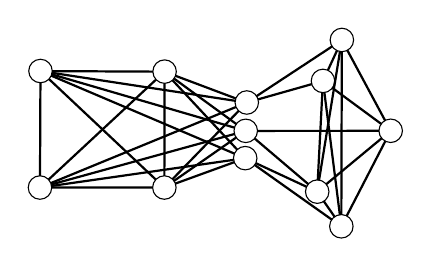
\begin{tikzpicture}[scale = 10]
\tikzstyle{VertexStyle}=[shape = circle, minimum size = 1pt, inner sep = 3pt,
draw]
\Vertex[x = 0.25085711479187, y = 0.92838092893362, L = \tiny {}]{v0}
\Vertex[x = 0.0932380929589272, y = 0.929142817854881, L = \tiny {}]{v1}
\Vertex[x = 0.250571489334106, y = 0.781142801046371, L = \tiny {}]{v2}
\Vertex[x = 0.092571459710598, y = 0.781142845749855, L = \tiny {}]{v3}
\Vertex[x = 0.355238050222397, y = 0.889142841100693, L = \tiny {}]{v4}
\Vertex[x = 0.353904783725739, y = 0.853142827749252, L = \tiny {}]{v5}
\Vertex[x = 0.353238135576248, y = 0.818476170301437, L = \tiny {}]{v6}
\Vertex[x = 0.476000010967255, y = 0.968571435660124, L = \tiny {}]{v7}
\Vertex[x = 0.537999987602234, y = 0.853238105773926, L = \tiny {}]{v8}
\Vertex[x = 0.444666564464569, y = 0.77590474486351, L = \tiny {}]{v9}
\Vertex[x = 0.475333333015442, y = 0.731904745101929, L = \tiny {}]{v10}
\Vertex[x = 0.451999962329865, y = 0.916571423411369, L = \tiny {}]{v11}
\Edge[](v0)(v1)
\Edge[](v2)(v1)
\Edge[](v3)(v1)
\Edge[](v0)(v3)
\Edge[](v2)(v3)
\Edge[](v2)(v0)
\Edge[](v4)(v2)
\Edge[](v5)(v2)
\Edge[](v6)(v2)
\Edge[](v4)(v0)
\Edge[](v5)(v0)
\Edge[](v6)(v0)
\Edge[](v4)(v1)
\Edge[](v5)(v1)
\Edge[](v6)(v1)
\Edge[](v4)(v3)
\Edge[](v5)(v3)
\Edge[](v6)(v3)
\Edge[](v8)(v7)
\Edge[](v9)(v7)
\Edge[](v10)(v7)
\Edge[](v11)(v7)
\Edge[](v9)(v8)
\Edge[](v10)(v8)
\Edge[](v11)(v8)
\Edge[](v10)(v9)
\Edge[](v11)(v9)
\Edge[](v11)(v10)
\Edge[](v4)(v7)
\Edge[](v4)(v11)
\Edge[](v6)(v9)
\Edge[](v6)(v10)
\Edge[](v5)(v8)
\Edge[](v5)(v9)
\end{tikzpicture}}}}\qquad\qquad
\subfloat[$\Delta=7$]{
{\parbox{5cm}{

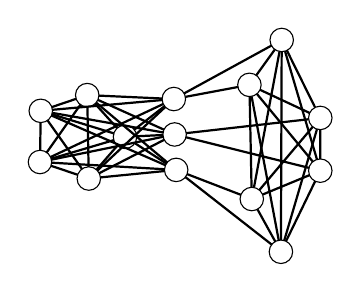
\begin{tikzpicture}[scale = 5]
\tikzstyle{VertexStyle}=[shape = circle, minimum size = 1pt, inner sep = 3pt,
draw]
\Vertex[x = 0.751999914646149, y = 0.724000096321106, L = \tiny {}]{v0}
\Vertex[x = 0.751999974250793, y = 0.590000092983246, L = \tiny {}]{v1}
\Vertex[x = 0.652000069618225, y = 0.38400000333786, L = \tiny {}]{v2}
\Vertex[x = 0.578000009059906, y = 0.51800012588501, L = \tiny {}]{v3}
\Vertex[x = 0.572000086307526, y = 0.808000028133392, L = \tiny {}]{v4}
\Vertex[x = 0.0419999808073044, y = 0.742000013589859, L = \tiny {}]{v5}
\Vertex[x = 0.0399999916553497, y = 0.612000048160553, L = \tiny {}]{v6}
\Vertex[x = 0.163999989628792, y = 0.569999992847443, L = \tiny {}]{v7}
\Vertex[x = 0.25600004196167, y = 0.676000028848648, L = \tiny {}]{v8}
\Vertex[x = 0.159999996423721, y = 0.782000005245209, L = \tiny {}]{v9}
\Vertex[x = 0.653999924659729, y = 0.921999998390675, L = \tiny {}]{v10}
\Vertex[x = 0.379999995231628, y = 0.771999999880791, L = \tiny {}]{v11}
\Vertex[x = 0.381999999284744, y = 0.682000011205673, L = \tiny {}]{v12}
\Vertex[x = 0.386000007390976, y = 0.592000007629395, L = \tiny {}]{v13}
\Edge[](v0)(v4)
\Edge[](v1)(v4)
\Edge[](v2)(v4)
\Edge[](v3)(v4)
\Edge[](v0)(v3)
\Edge[](v1)(v3)
\Edge[](v2)(v3)
\Edge[](v0)(v2)
\Edge[](v1)(v2)
\Edge[](v0)(v1)
\Edge[](v5)(v6)
\Edge[](v5)(v7)
\Edge[](v5)(v8)
\Edge[](v5)(v9)
\Edge[](v6)(v7)
\Edge[](v6)(v8)
\Edge[](v6)(v9)
\Edge[](v7)(v8)
\Edge[](v7)(v9)
\Edge[](v8)(v9)
\Edge[](v0)(v10)
\Edge[](v1)(v10)
\Edge[](v2)(v10)
\Edge[](v3)(v10)
\Edge[](v4)(v10)
\Edge[](v5)(v11)
\Edge[](v6)(v11)
\Edge[](v7)(v11)
\Edge[](v8)(v11)
\Edge[](v9)(v11)
\Edge[](v5)(v12)
\Edge[](v6)(v12)
\Edge[](v7)(v12)
\Edge[](v8)(v12)
\Edge[](v9)(v12)
\Edge[](v5)(v13)
\Edge[](v6)(v13)
\Edge[](v7)(v13)
\Edge[](v8)(v13)
\Edge[](v9)(v13)
\Edge[](v11)(v10)
\Edge[](v11)(v4)
\Edge[](v12)(v0)
\Edge[](v12)(v1)
\Edge[](v13)(v3)
\Edge[](v13)(v2)
\end{tikzpicture}}}}\qquad\qquad
\subfloat[$\Delta=7$~~~~~~~~~~~~~~~]{
{\parbox{5cm}{

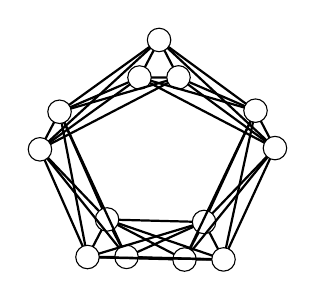
\begin{tikzpicture}[scale = 10]
\tikzstyle{VertexStyle}=[shape = circle, minimum size = 1pt, inner sep = 3pt,
draw]
\Vertex[x = 0.257401078939438, y = 0.729450404644012, L = \tiny {}]{v0}
\Vertex[x = 0.232565611600876, y = 0.681758105754852, L = \tiny {}]{v1}
\Vertex[x = 0.383801102638245, y = 0.820650428533554, L = \tiny {}]{v2}
\Vertex[x = 0.358965694904327, y = 0.772958129644394, L = \tiny {}]{v3}
\Vertex[x = 0.40850430727005, y = 0.773111909627914, L = \tiny {}]{v4}
\Vertex[x = 0.506290018558502, y = 0.730872631072998, L = \tiny {}]{v5}
\Vertex[x = 0.530993163585663, y = 0.683334112167358, L = \tiny {}]{v6}
\Vertex[x = 0.440956592559814, y = 0.589494824409485, L = \tiny {}]{v7}
\Vertex[x = 0.416121125221252, y = 0.541802525520325, L = \tiny {}]{v8}
\Vertex[x = 0.46565979719162, y = 0.541956305503845, L = \tiny {}]{v9}
\Vertex[x = 0.317756593227386, y = 0.592694818973541, L = \tiny {}]{v10}
\Vertex[x = 0.292921125888824, y = 0.545002520084381, L = \tiny {}]{v11}
\Vertex[x = 0.342459797859192, y = 0.545156300067902, L = \tiny {}]{v12}
\Edge[](v1)(v0)
\Edge[](v3)(v2)
\Edge[](v4)(v2)
\Edge[](v4)(v3)
\Edge[](v6)(v5)
\Edge[](v8)(v7)
\Edge[](v9)(v7)
\Edge[](v9)(v8)
\Edge[](v11)(v10)
\Edge[](v12)(v10)
\Edge[](v12)(v11)
\Edge[](v2)(v0)
\Edge[](v3)(v0)
\Edge[](v4)(v0)
\Edge[](v2)(v1)
\Edge[](v3)(v1)
\Edge[](v4)(v1)
\Edge[](v2)(v5)
\Edge[](v3)(v5)
\Edge[](v4)(v5)
\Edge[](v2)(v6)
\Edge[](v3)(v6)
\Edge[](v4)(v6)
\Edge[](v5)(v7)
\Edge[](v6)(v7)
\Edge[](v5)(v9)
\Edge[](v6)(v9)
\Edge[](v5)(v8)
\Edge[](v6)(v8)
\Edge[](v10)(v8)
\Edge[](v11)(v8)
\Edge[](v12)(v8)
\Edge[](v10)(v7)
\Edge[](v11)(v7)
\Edge[](v12)(v7)
\Edge[](v10)(v9)
\Edge[](v11)(v9)
\Edge[](v12)(v9)
\Edge[](v10)(v1)
\Edge[](v11)(v1)
\Edge[](v12)(v1)
\Edge[](v10)(v0)
\Edge[](v11)(v0)
\Edge[](v12)(v0)
\end{tikzpicture}}}}\qquad\qquad
\subfloat[$\Delta=8$~~~~~~~~~~~~~~~]{
{\parbox{5cm}{

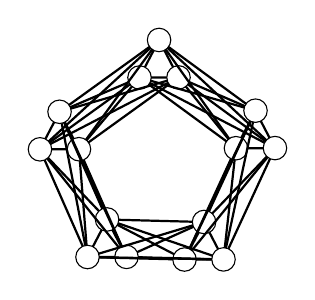
\begin{tikzpicture}[scale = 10]
\tikzstyle{VertexStyle}=[shape = circle, minimum size = 1pt, inner sep = 3pt,
draw]
\Vertex[x = 0.257401078939438, y = 0.729450404644012, L = \tiny {}]{v0}
\Vertex[x = 0.232565611600876, y = 0.681758105754852, L = \tiny {}]{v1}
\Vertex[x = 0.282104313373566, y = 0.681911885738373, L = \tiny {}]{v2}
\Vertex[x = 0.383801102638245, y = 0.820650428533554, L = \tiny {}]{v3}
\Vertex[x = 0.358965694904327, y = 0.772958129644394, L = \tiny {}]{v4}
\Vertex[x = 0.40850430727005, y = 0.773111909627914, L = \tiny {}]{v5}
\Vertex[x = 0.506290018558502, y = 0.730872631072998, L = \tiny {}]{v6}
\Vertex[x = 0.48145455121994, y = 0.683180332183838, L = \tiny {}]{v7}
\Vertex[x = 0.530993163585663, y = 0.683334112167358, L = \tiny {}]{v8}
\Vertex[x = 0.440956592559814, y = 0.589494824409485, L = \tiny {}]{v9}
\Vertex[x = 0.416121125221252, y = 0.541802525520325, L = \tiny {}]{v10}
\Vertex[x = 0.46565979719162, y = 0.541956305503845, L = \tiny {}]{v11}
\Vertex[x = 0.317756593227386, y = 0.592694818973541, L = \tiny {}]{v12}
\Vertex[x = 0.292921125888824, y = 0.545002520084381, L = \tiny {}]{v13}
\Vertex[x = 0.342459797859192, y = 0.545156300067902, L = \tiny {}]{v14}
\Edge[](v2)(v1)
\Edge[](v2)(v0)
\Edge[](v1)(v0)
\Edge[](v4)(v3)
\Edge[](v5)(v3)
\Edge[](v5)(v4)
\Edge[](v7)(v6)
\Edge[](v8)(v6)
\Edge[](v8)(v7)
\Edge[](v10)(v9)
\Edge[](v11)(v9)
\Edge[](v11)(v10)
\Edge[](v13)(v12)
\Edge[](v14)(v12)
\Edge[](v14)(v13)
\Edge[](v3)(v0)
\Edge[](v4)(v0)
\Edge[](v5)(v0)
\Edge[](v3)(v2)
\Edge[](v4)(v2)
\Edge[](v5)(v2)
\Edge[](v3)(v1)
\Edge[](v4)(v1)
\Edge[](v5)(v1)
\Edge[](v3)(v6)
\Edge[](v4)(v6)
\Edge[](v5)(v6)
\Edge[](v3)(v7)
\Edge[](v4)(v7)
\Edge[](v5)(v7)
\Edge[](v3)(v8)
\Edge[](v4)(v8)
\Edge[](v5)(v8)
\Edge[](v6)(v9)
\Edge[](v7)(v9)
\Edge[](v8)(v9)
\Edge[](v6)(v11)
\Edge[](v7)(v11)
\Edge[](v8)(v11)
\Edge[](v6)(v10)
\Edge[](v7)(v10)
\Edge[](v8)(v10)
\Edge[](v12)(v10)
\Edge[](v13)(v10)
\Edge[](v14)(v10)
\Edge[](v12)(v9)
\Edge[](v13)(v9)
\Edge[](v14)(v9)
\Edge[](v12)(v11)
\Edge[](v13)(v11)
\Edge[](v14)(v11)
\Edge[](v12)(v2)
\Edge[](v13)(v2)
\Edge[](v14)(v2)
\Edge[](v12)(v1)
\Edge[](v13)(v1)
\Edge[](v14)(v1)
\Edge[](v12)(v0)
\Edge[](v13)(v0)
\Edge[](v14)(v0)
\end{tikzpicture}}}}
\caption{Counterexamples to the Borodin-Kostochka Conjecture for small
$\Delta$.}
\label{fig:SmallCE}
\end{figure}


\begin{conjecture}[Borodin and Kostochka \cite{borodin1977upper}]
Every graph with $\Delta \geq 9$ satisfies $\chi \leq \max\{\omega, \Delta - 1\}$.
\end{conjecture}

Note that another way of stating this is that for $\Delta \geq 9$, the only obstruction to $(\Delta-1)$-coloring is a $K_\Delta$. In the same paper, Borodin and Kostochka prove the following weaker statement.

\begin{thm}[Borodin and Kostochka \cite{borodin1977upper}]\label{BorodinKostochkaBK}
Every graph satisfying $\chi \geq \Delta \geq 7$ contains a $K_{\floor{\frac{\Delta + 1}{2}}}$.
\end{thm}

The proof is quite simple once you have a decomposition lemma of Lov\'{a}sz from the 1960's \cite{lovasz1966decomposition}.

\begin{lem}[Lov\'{a}sz
\cite{lovasz1966decomposition}]\label{LovaszDecomposition} Let $G$ be a graph and $r_1, \ldots, r_k \in \IN$ such that $\sum_{i=1}^k r_i \geq \Delta(G) + 1 - k$. 
Then $V(G)$ can be partitioned into sets $V_1, \ldots, V_k$ such that $\Delta(G[V_i]) \leq r_i$ for each $i \in \irange{k}$.
\end{lem}
\begin{proof}
For a partition $P \DefinedAs \parens{V_1, \ldots, V_k}$ of $V(G)$ let
			\[f(P) \DefinedAs \sum_{i=1}^k \parens{\size{G[V_i]} - r_i\card{V_i}}.\]

\noindent Let $P \DefinedAs \parens{V_1, \ldots, V_k}$ be a partition of $V(G)$
minimizing $f(P)$.  Suppose there is $i \in \irange{k}$ and $x \in V_i$ with
$d_{V_i}(x) > r_i$. Since $\sum_{i=1}^k r_i \geq \Delta(G) + 1 - k$, there is
some $j \neq i$ such that $d_{V_j}(x) \leq r_j$ and thus moving $x$ from $V_i$ to
$V_j$ gives a new partition violating minimality of $f(P)$.  Hence
$\Delta(G[V_i]) \leq r_i$ for each $i \in \irange{k}$.
\end{proof}

Now to prove Borodin and Kostochka's result, let $G$ be a graph with $\chi \geq
\Delta \geq 7$ and use $r_1 \DefinedAs \ceil{\frac{\Delta - 1}{2}}$ and $r_2
\DefinedAs \floor{\frac{\Delta - 1}{2}}$ in Lov\'{a}sz's lemma to get a
partition $(V_1, V_2)$ of $V(G)$ with $\Delta(G[V_i]) \leq r_i$ for each $i \in
\irange{2}$.  Since $r_1 + r_2 = \Delta - 1$ and $\chi \geq \Delta$, it
must be that $\chi(G[V_i]) \geq r_i + 1$ for some $i \in \irange{2}$. But
$\Delta \geq 7$, so $r_i \geq 3$ and hence by Brooks' theorem $G[V_i]$ contains
a $K_{\floor{\frac{\Delta + 1}{2}}}$.

A decade later, Catlin \cite{CatlinAnotherBound} showed that bumping the $\Delta(G) + 1$ to $\Delta(G) + 2$ allowed for shuffling vertices from one partition set to another and thereby 
proving stronger decomposition results. A few years later Kostochka \cite{KostochkaTriangleFree} modified Catlin's algorithm to show that every triangle-free graph $G$ can be 
colored with at most $\frac23 \Delta(G) + 2$ colors.  In \cite{rabern2010destroying}, we generalized Kostochka's modification to prove the following.

\begin{replem}{DestroyLemma}[Rabern \cite{rabern2010destroying}]
Let $G$ be a graph and $r_1, \ldots, r_k \in \IN$ such that $\sum_{i=1}^k r_i \geq \Delta(G) + 2 - k$. 
Then $V(G)$ can be partitioned into sets $V_1, \ldots, V_k$ such that $\Delta(G[V_i]) \leq r_i$ and $G[V_i]$ contains no incomplete $r_i$-regular components for each $i \in \irange{k}$.
\end{replem}

Setting $k = \left \lceil \frac{\Delta(G) + 2}{3} \right \rceil$ and $r_i = 2$
for each $i$ gives a slightly more general form of Kostochka's triangle-free
coloring result.

\begin{repcor}{TrianglesAndPaths}[Rabern \cite{rabern2010destroying}]
The vertex set of any graph $G$ can be partitioned into $\left \lceil \frac{\Delta(G) + 2}{3} \right \rceil$ sets, each of which induces a disjoint union of triangles and paths.
\end{repcor}

For coloring, this actually gives the bound $\chi(G) \leq 2  \left \lceil \frac{\Delta(G) + 2}{3} \right \rceil$ for triangle free graphs.  
To get $\frac23 \Delta(G) + 2$, just use $r_k = 0$ when $\Delta \equiv 2 (\text{mod } 3)$. 
Similarly, for any $r \geq 2$, setting $k = \left \lceil \frac{\Delta(G) + 2}{r + 1} \right \rceil$ and $r_i = r$ for each $i$ gives the following.
\begin{repcor}{NoKrPlusOne}[Rabern \cite{rabern2010destroying}]
Fix $r \geq 2$.  The vertex set of any $K_{r + 1}$-free graph $G$ can be partitioned into $\left \lceil \frac{\Delta(G) + 2}{r + 1} \right \rceil$ sets each inducing an $(r-1)$-degenerate subgraph with maximum degree at most $r$.
\end{repcor}
In fact, we proved a lemma stronger than Lemma \ref{DestroyLemma} allowing us
to forbid a larger class of components coming from any so-called \emph{$r$-permissible collection}. In section \ref{ShuffleHeightSection} we will explore a result that both simplifies and generalizes this latter result.

Also in the 1980's, Kostochka proved the following using a complicated recoloring argument together with a technique for reducing $\Delta$ in a counterexample 
based on hitting every maximum clique with an independent set.

\begin{thm}[Kostochka \cite{kostochkaRussian}]\label{KostochkaBK}
Every graph satisfying $\chi \geq \Delta$ contains a $K_{\Delta - 28}$.
\end{thm}

Kostochka \cite{kostochkaRussian} proved the following result which shows that
graphs having clique number sufficiently close to their maximum degree contain
an independent set hitting every maximum clique. In \cite{rabernhitting} we
improved the antecedent to $\omega \geq \frac34(\Delta + 1)$.  Finally, King  \cite{KingHitting} made the result tight.

\begin{replem}{KostochkaHitting}[Kostochka \cite{kostochkaRussian}]
If $G$ is a graph satisfying $\omega \geq \Delta + \frac32 - \sqrt{\Delta}$,
then $G$ contains an independent set $I$ such that $\omega(G - I) < \omega(G)$.
\end{replem}
\begin{replem}{RabernHitting}[Rabern \cite{rabernhitting}]
If $G$ is a graph satisfying $\omega \geq \frac34 (\Delta + 1)$,
then $G$ contains an independent set $I$ such that $\omega(G - I) < \omega(G)$.
\end{replem}
\begin{replem}{HittingMaxCliques}[King \cite{KingHitting}]
If $G$ is a graph satisfying $\omega > \frac23 (\Delta + 1)$, then $G$ contains
an independent set $I$ such that $\omega(G - I) < \omega(G)$.
\end{replem}

If $G$ is a vertex critical graph satisfying $\omega > \frac23 (\Delta + 1)$ and
we expand the independent set $I$ produced by Lemma \ref{HittingMaxCliques} to a
maximal independent set $M$ and remove $M$ from $G$, we see that $\Delta(G-M)
\leq \Delta(G) - 1$, $\chi(G-M) = \chi(G) - 1$ and $\omega(G - M) = \omega(G) - 1$. Using this, the proof of many coloring results can be reduced to the case of the
smallest $\Delta$ for which they work. In Chapter
\ref{ReductionChapter}, we give three such applications.

A little after Kostochka proved his bound, Mozhan \cite{mozhan1983}
used a function minimization and vertex shuffling procedure different than, but related to Catlin's, to prove the following.  

\begin{thm}[Mozhan \cite{mozhan1983}]\label{MozhanTwoThirdsBK}
Every graph satisfying $\chi \geq \Delta \geq 10$ contains a $K_{\floor{\frac{2\Delta + 1}{3}}}$.
\end{thm}

Finally, in his dissertation Mozhan proved the following.  We don't know the
method of proof as we were unable to obtain a copy of his dissertation. 
However, we suspect the method is a more complicated version of the above proof.

\begin{thm}[Mozhan]\label{MozhanBK}
Every graph satisfying $\chi \geq \Delta \geq 31$ contains a $K_{\Delta - 3}$.
\end{thm}

In \cite{rabern2010a}, we used part of Mozhan's method to prove the following result.  For a graph $G$ let $\mathcal{H}(G)$ be the subgraph of $G$ induced on the vertices of degree at least $\chi(G)$.

\begin{thm}[Rabern \cite{rabern2010a}]\label{TheoremM}
$K_{\chi(G)}$ is the only vertex critical graph $G$ with $\chi(G) \geq \Delta(G) \geq 6$ and $\omega(\mathcal{H}(G)) \leq \left \lfloor \frac{\Delta(G)}{2} \right \rfloor - 2$.
\end{thm}

Setting $\omega(\mathcal{H}(G)) = 1$ proved a conjecture of Kierstead and Kostochka \cite{kierstead2009ore}.

\begin{cor}[Rabern \cite{rabern2010a}]\label{CorollaryN}
$K_{\chi(G)}$ is the only vertex critical graph $G$ with $\chi(G) \geq \Delta(G) \geq 6$ such that $\mathcal{H}(G)$ is edgeless.
\end{cor}

In joint work with Kostochka and Stiebitz \cite{krs_one}, we generalized and improved this result, again using Mozhan's technique.  
In section \ref{ShuffleLowsSection}, we will improve these results further and simplify the proofs by using Catlin's vertex shuffling algorithm in place of Mozhan's.

In 1999, Reed used probabilistic methods to prove that the Borodin-Kostochka conjecture holds for graphs with very large maximum degree.

\begin{thm}[Reed \cite{reed1999strengthening}]\label{ReedBK}
Every graph satisfying $\chi \geq \Delta \geq 10^{14}$ contains a $K_\Delta$.
\end{thm}

A lemma from Reed's proof of the above theorem is generally useful.

\begin{lem}[Reed \cite{reed1999strengthening}]\label{ReedsLemma}
Let $G$ be a critical graph satisfying $\chi = \Delta \geq 9$ having the minimum number of vertices.  If $H$ is a $K_{\Delta - 1}$ in $G$, then any vertex in $G - H$ has at most $4$ neighbors in $H$.  In particular, the $K_{\Delta - 1}$'s in $G$ are pairwise disjoint.
\end{lem}

In Chapter \ref{APrioriWowChapter}, we improve this lemma by showing that under
the same hypotheses, any vertex in $G - H$ has at most $1$ neighbor in $H$.  Moreover, we lift the result out of the context of a minimal counterexample to graphs satisfying a certain criticality condition---we refer to such graphs as mules.  This allows meaningful results to be proved for values of $\Delta$ less than $9$.  Also in Chapter \ref{APrioriWowChapter}, we prove that the following, prima facie weaker, conjecture is equivalent to the Borodin-Kostochka conjecture.

\begin{conjecture}[Cranston and Rabern \cite{mules}] 
If $G$ is a graph with $\chi = \Delta = 9$, then $\join{K_3}{\overline{K}_6}
\subseteq G$.
\end{conjecture}

At the core of these results are the list coloring lemmas proved in section
\ref{ListColoringChapter}.  There we classify graphs of the form $\join{A}{B}$
that are not $f$-choosable where $f(v) \DefinedAs d(v) - 1$ for each vertex
$v$.  In Chapter \ref{ClawFreeChapter} we use these list coloring results
together with Chudnovsky and Seymour's decomposition theorem for claw-free graphs \cite{chudnovsky2005structure} and our proof in \cite{rabern2011strengthening} of the Borodin-Kostochka conjecture for line graphs of multigraphs to prove the conjecture for claw-free graphs.

\begin{thm}[Cranston and Rabern \cite{cranstonrabernclaw}]
Every claw-free graph with $\Delta\geq 9$ satisfies $\chi \leq \max\set{\omega, \Delta - 1}$.
\end{thm}

In Chapter \ref{StrongColoringChapter}, we adapt a recoloring trick
previously used for strong coloring and prove the following.

\begin{repcor}{TwoThirdsCliqueCor}
Every graph with $\chi \geq \Delta \geq 9$ such that every
vertex is in a clique on $\frac23\Delta + 2$ vertices contains $K_\Delta$.
\end{repcor}

Using this we show that to prove the Borodin-Kostochka conjecture it is enough
to prove it for irregular graphs; more precisely, we prove the following.

\begin{repthm}{IrregularReduction}
Every graph satisfying $\chi \geq \Delta = k \geq 9$ either
contains $K_k$ or contains an irregular critical subgraph satisfying $\chi
= \Delta = k - 1$.
\end{repthm}

In particular, the Borodin-Kostochka conjecture would follow from the following.
This is at least somewhat plausible since the only known critical (or connected
even) counterexample to Borodin-Kostochka for $\Delta = 8$ is regular (see
Figure \ref{fig:M_8}).

\begin{repconjecture}{EightRegular}
Every critical graph satisfying $\chi \geq \Delta = 8$ is regular.
\end{repconjecture}

As our final application of the recoloring trick, we prove the following bounds on the chromatic number.  The first generalizes the result of Beutelspacher and Hering \cite{beutelspacher1984minimal} that the Borodin-Kostochka conjecture holds for graphs with independence number at most two.  This result was generalized in another direction in \cite{cranstonrabernclaw} (also Chapter \ref{ClawFreeChapter}) where the conjecture was proved for claw-free graphs.

\begin{repthm}{AlphaBound}
Every graph satisfies $\chi \leq \max\set{\omega, \Delta - 1, 4\alpha}$.
\end{repthm}

The second bound shows that the Borodin-Kostochka conjecture holds for graphs with maximum degree on the order of the square root of their order.  This improves on prior bounds of $\Delta > \frac{n + 1}{2}$ from Beutelspacher and Hering \cite{beutelspacher1984minimal} and $\Delta > \frac{n-6}{3}$ of Naserasr \cite{naserasr}.

\begin{repthm}{OrderBound}
Every graph satisfies $\chi \leq \max\set{\omega, \Delta - 1, \ceil{\frac{15 + \sqrt{48n + 73}}{4}}}$.
\end{repthm}

Borodin and Kostochka also conjectured \cite{PersonalComms} that
their conjecture holds for list coloring. In Chapter \ref{ChoiceLargeDeltaChapter}, we prove that this conjecture holds for large $\Delta$.

\begin{conjecture}[Borodin and Kostochka \cite{PersonalComms}]\label{BKList}
Every graph with $\Delta \geq 9$ satisfies $\chi_l \leq \max\{\omega, \Delta -
1\}$.
\end{conjecture}


\chapter{BROOKS' THEOREM}\label{BrooksChapter}

In Chapter \ref{APrioriWowChapter} we will rely heavily on the technique of
adding edges to a proper induced subgraph of a minimum counterexample.  We first
learned of this technique when reading Reed's proof of the Borodin-Kostochka
conjecture for large $\Delta$ (see \cite{reed1999strengthening}). To introduce
the idea we give a short proof of Brooks' theorem. The proof is completely
different from Lov\'{a}sz's short proof in \cite{Lovasz1975269}. We first reduce to the cubic case and then add edges to a proper induced
subgraph to get a coloring we can complete. The reduction to the cubic case is an immediate consequence of more
general lemmas on hitting all maximum cliques with an independent set that we
prove in Chapter \ref{ReductionChapter} (see also \cite{kostochkaRussian},
\cite{rabernhitting} and \cite{KingHitting}). Additionally, this reduction was
demonstrated by Tverberg in \cite{tverberg1983brooks}.  One
interesting feature of the proof is that it doesn't use any connectivity
concepts.
We'll give two versions of the proof, the first is shorter but uses the extra idea of excluding diamonds ($K_4$ less an edge).

\begin{thm}[Brooks \cite{brooks1941colouring}]
Every graph satisfies $\chi \leq \max\set{3, \omega, \Delta}$.
\end{thm}
\begin{proof}
Suppose the theorem is false and choose a counterexample $G$ minimizing
$\card{G}$.  Put $\Delta \DefinedAs \Delta(G)$. Using minimality of $\card{G}$,
we see that $\chi(G - v) \leq \Delta$ for all $v \in
V(G)$. In particular, $G$ is $\Delta$-regular.

First, suppose $G$ is $3$-regular.  If $G$ contains a diamond $D$, then we may $3$-color $G-D$ and easily extend the coloring to $D$ by first coloring the nonadjacent vertices in $D$ the same.  So, $G$ doesn't contain diamonds. Since $G$ is not a forest it contains an induced cycle $C$. Since $K_4 \not
\subseteq G$ we have $\card{N(C)} \geq 2$. So, we may take different $x, y \in N(C)$ and put $H \DefinedAs G - C$ if $x$ is adjacent to $y$ and $H \DefinedAs (G-C) + xy$ otherwise.  Then, $H$ doesn't contain $K_4$ as $G$ doesn't contain diamonds. By minimality of $\card{G}$, $H$ is $3$-colorable. That is, we have a $3$-coloring of $G - C$ where $x$ and $y$ receive different colors.  We can easily extend this partial
coloring to all of $G$ since each vertex of $C$ has a set of two available
colors and some pair of vertices in $C$ get different sets.  

Hence we must have $\Delta \geq 4$. Consider a $\Delta$-coloring of $G-v$ for some $v \in V(G)$.  Each color must be used on every $K_{\Delta}$ in $G-v$ and hence some color must be used on every $K_{\Delta}$ in $G$.  Let $M$ be such a color class expanded to a maximal independent set.  Then $\chi(G-M) = \chi(G) - 1 = \Delta > \max\set{3, \omega(G-M), \Delta(G-M)}$, a contradiction.
\end{proof}

Here is the other version, not excluding diamonds and doing the reduction differently.

\begin{thm}[Brooks \cite{brooks1941colouring}]
Every graph $G$ with $\chi(G) = \Delta(G) + 1 \geq 4$ contains
$K_{\Delta(G) + 1}$.
\end{thm}
\begin{proof}
Suppose the theorem is false and choose a counterexample $G$ minimizing
$\card{G}$.  Put $\Delta \DefinedAs \Delta(G)$. Using minimality of $\card{G}$,
we see that $\chi(G - v) \leq \Delta$ for all $v \in
V(G)$. In particular, $G$ is $\Delta$-regular.

First, suppose $\Delta \geq 4$.  Pick $v \in V(G)$ and let $w_1, \ldots,
w_\Delta$ be $v$'s neighbors. Since $K_{\Delta + 1} \not \subseteq G$, by
symmetry we may assume that $w_2$ and $w_3$ are not adjacent. Choose a $(\Delta
+ 1)$-coloring $\set{\set{v}, C_1, \ldots, C_\Delta}$ of $G$ where $w_i \in
C_i$ so as to maximize $\card{C_1}$.  Then $C_1$ is a maximal independent set in
$G$ and in particular, with $H \DefinedAs G - C_1$, we have $\chi(H) =
\chi(G) - 1 = \Delta = \Delta(H) + 1 \geq 4$.  By minimality of $\card{G}$, we
get $K_\Delta \subseteq H$.  But $\set{\set{v}, C_2, \ldots, C_\Delta}$ is a
$\Delta$-coloring of $H$, so any $K_\Delta$ in $H$ must contain $v$ and hence
$w_2$ and $w_3$, a contradiction.

Therefore $G$ is $3$-regular.  Since $G$ is not a forest it contains an induced
cycle $C$.  Put $T \DefinedAs N(C)$.  Then $\card{T} \geq 2$ since $K_4 \not
\subseteq G$.  Take different $x, y \in T$ and put $H_{xy} \DefinedAs G - C$ if
$x$ is adjacent to $y$ and $H_{xy} \DefinedAs (G-C) + xy$ otherwise.  Then, by
minimality of $\card{G}$, either $H_{xy}$ is $3$-colorable or adding $xy$
created a $K_4$ in $H_{xy}$.

Suppose the former happens.  Then we have a $3$-coloring of $G - C$
where $x$ and $y$ receive different colors.  We can easily extend this partial
coloring to all of $G$ since each vertex of $C$ has a set of two available
colors and some pair of vertices in $C$ get different sets. 

Whence adding $xy$ created a $K_4$, call it $A$, in $H_{xy}$.  We conclude that
$T$ is independent and each vertex in $T$ has exactly one neighbor in $C$.  Hence
$\card{T} \geq \card{C} \geq 3$. Pick $z \in T - \set{x,y}$.  Then $x$ is
contained in a $K_4$, call it $B$, in $H_{xz}$.  Since $d(x) = 3$, we must have
$A - \set{x,y} = B - \set{x, z}$.  But then any $w \in A - \set{x,y}$ has degree
at least $4$, a contradiction.
\end{proof}

\chapter{DOING THE VERTEX SHUFFLE}\label{VertexShuffleChapter}
\begin{center}
\emph{The material in this chapter appeared in \cite{rabern2012partitioning}, \cite{rabern2010destroying} and \cite{partitionnote}.}
\end{center}

Let $\G$ be the collection of all finite simple connected graphs. 
For a graph $G$, $x \in V(G)$ and $D \subseteq V(G)$ we use the notation $N_D(x) \DefinedAs N(x) \cap D$ and $d_D(x) \DefinedAs \card{N_D(x)}$. 
Let $\fancy{C}_G$ be the components of $G$ and $c(G) \DefinedAs
\card{\fancy{C}_G}$. If $\func{h}{\G}{\IN}$, we define $h$ for any graph as
$h(G) \DefinedAs \sum_{D \in \fancy{C}_G} h(D)$.  An
\emph{ordered partition} of $G$ is a sequence $\parens{V_1, V_2, \ldots, V_k}$ where the $V_i$
are pairwise disjoint and cover $V(G)$.  Note that we allow the $V_i$ to be
empty.  When there is no possibility of ambiguity, we call such a sequence a
\emph{partition}.

\section{Coloring when the high vertex subgraph has small
cliques}\label{ShuffleLowsSection}

In \cite{kierstead2009ore} Kierstead and Kostochka investigated the Brooks bound
with the Ore-degree $\theta$ in place of $\Delta$.

\begin{defn}
The \emph{Ore-degree} of an edge $xy$ in a graph $G$ is $\theta(xy) \DefinedAs d(x) + d(y)$.  The \emph{Ore-degree} of a graph $G$ is $\theta(G) \DefinedAs \max_{xy \in E(G)}\theta(xy)$.
\end{defn}

\begin{thm}[Kierstead and Kostochka \cite{kierstead2009ore} 2010]
If $G$ is a graph with $\chi(G) \geq \floor{\frac{\theta(G)}{2}} + 1 \geq 7$ then $G$ contains $K_{\chi(G)}$.
\end{thm}

This statement about Ore-degree is equivalent to the following statement about vertex critical graphs.

\begin{thm}[Kierstead and Kostochka \cite{kierstead2009ore} 2010]
The only vertex critical graph $G$ with $\chi(G) \geq \Delta(G) \geq 7$ such that $\fancy{H}(G)$ is edgeless is $K_{\chi(G)}$.
\end{thm}

In \cite{rabern2010a}, we improved the $7$ to $6$ by proving the following generalization.

\begin{thm}[Rabern 2012 \cite{rabern2010a}]
The only vertex critical graph $G$ with $\chi(G) \geq \Delta(G) \geq 6$ and $\omega(\fancy{H}(G)) \leq \floor{\frac{\Delta(G)}{2}} - 2$ is $K_{\chi(G)}$.
\end{thm}

This result and those in \cite{rabern2010b} were improved by Kostochka, Rabern and Stiebitz in \cite{krs_one}.  In particular, the following was proved.

\begin{thm}[Kostochka, Rabern and Stiebitz \cite{krs_one}
2012]\label{krs_one_main} The only vertex critical graphs $G$ with $\chi(G) \geq
\Delta(G) \geq 5$ such that $\fancy{H}(G)$ is edgeless are $K_{\chi(G)}$ and $O_5$.
\end{thm}

\begin{figure}[h]
\centering
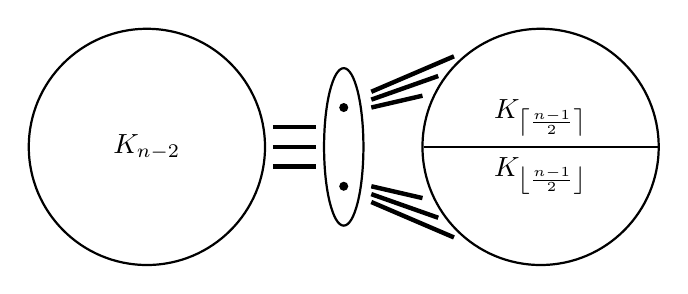
\begin{tikzpicture}[scale = 1]

\node[circle, minimum width=3cm, thick, draw] (L) at (0,0) {$K_{n-2}$};
\node[ellipse, minimum height=2cm, minimum width=0.5cm, thick, draw] (M) at (2.5,0) {};      
\node[circle split, minimum width=3cm, thick, draw] (R) at (5,0) 
{$K_{\ceil{\frac{n-1}{2}}}$ \nodepart{lower} $K_{\floor{\frac{n-1}{2}}}$};
\node[circle, inner sep =1pt, fill, draw] (P1) at (2.5,-0.5) {};
\node[circle, inner sep =1pt, fill, draw] (P2) at (2.5,0.5) {};

\draw (L) (M) (R) (P1) (P2);
\draw[ultra thick] (1.6,-.25) -- (2.15,-.25);
\draw[ultra thick] (1.6,0) -- (2.15,0);
\draw[ultra thick] (1.6,.25) -- (2.15,.25);

\draw[ultra thick] (2.85,-.7) -- (3.9,-1.15);
\draw[ultra thick] (2.85,-.6) -- (3.7,-.9);
\draw[ultra thick] (2.85,-.5) -- (3.5,-.65);

\draw[ultra thick] (2.85,.7) -- (3.9,1.15);
\draw[ultra thick] (2.85,.6) -- (3.7,.9);
\draw[ultra thick] (2.85,.5) -- (3.5,.65);
\end{tikzpicture}
\caption{The graph $O_n$.}
\end{figure}


Here $O_n$ is the graph formed from the disjoint union of $K_n - xy$ and
$K_{n-1}$ by joining $\floor{\frac{n-1}{2}}$ vertices of the $K_{n-1}$ to $x$
and the other $\ceil{\frac{n-1}{2}}$ vertices of the $K_{n-1}$ to $y$ (see
Figure \ref{fig:reducer}). In \cite{rabern2012partitioning} we proved a result that implies all of the results in \cite{krs_one}. The proof replaces an algorithm of Mozhan \cite{mozhan1983} with the original, more general, algorithm of Catlin \cite{CatlinAnotherBound} on which it is based. This allows for a considerable simplification.   Moreover, we prove two preliminary partitioning results that are of independent interest.  
All coloring results follow from the first of these, the second is a generalization of a lemma due to Borodin \cite{borodin1976decomposition} (and independently Bollob\'as and Manvel \cite{bollobasManvel})
about partitioning a graph into degenerate subgraphs.  The following is the main
coloring result in \cite{rabern2012partitioning}.

\begin{cor}\label{MainShuffleColoringResult}
	Let $G$ be a vertex critical graph with $\chi(G) \geq \Delta(G) + 1 - p \geq 4$
	for some $p \in \IN$.  If $\omega(\fancy{H}(G)) \leq \frac{\chi(G) + 1}{p + 1} - 2$,
	then $G = K_{\chi(G)}$ or $G = O_5$.
\end{cor}

In the sections that follow we will prove this Corollary.  First, we give a
non-standard proof of Brooks' theorem to illustrate the technique.

\subsection{A weird proof of Brooks' theorem}
Let $G$ be a graph.  A partition $P \DefinedAs (V_0, V_1)$ of $V(G)$
will be called \emph{normal} if it achieves the minimum value of $(\Delta(G) -
1)\size{V_0} + \size{V_1}$.  Note that if $P$ is a normal partition, then
$\Delta(G[V_0]) \leq 1$ and $\Delta(G[V_1]) \leq \Delta(G) - 1$.  
The \emph{$P$-components} of $G$ are the components of $G[V_i]$ for $i \in
\irange{2}$.  A $P$-component is called an \emph{obstruction} if it is a
$K_2$ in $G[V_0]$ or a $K_{\Delta(G)}$ in $G[V_1]$ or an odd cycle in $G[V_1]$ when
$\Delta(G) = 3$.  A path $x_1x_2\cdots x_k$ is called \emph{$P$-acceptable} if
$x_1$ is contained in an obstruction and for different $i, j \in \irange{k}$, $x_i$ and
$x_j$ are in different $P$-components.  For a subgraph $H$ of $G$ and $x \in V(G)$, 
we put $N_H(x) \DefinedAs N(x) \cap V(H)$.

\begin{lem}\label{ObstructionFree}
Let $G$ be a graph with $\Delta(G) \geq 3$.  If $G$ doesn't contain
$K_{\Delta(G) + 1}$, then $V(G)$ has an obstruction-free normal partition.
\end{lem}
\begin{proof}
Suppose the lemma is false.  Among the normal partitions having the minimum
number of obstructions, choose $P \DefinedAs (V_0, V_1)$ and a
maximal $P$-acceptable path $x_1x_2\cdots x_k$ so as to minimize $k$.

Let $A$ and $B$ be the $P$-components containing $x_1$ and $x_k$ respectively.  
Put $X \DefinedAs N_A(x_k)$. First, suppose $\card{X} = 0$.  Then moving $x_1$ to the
other part of $P$ creates another normal partition $P'$ having the minimum number of
obstructions.  But $x_2x_3\cdots x_k$ is a maximal $P'$-acceptable path,
violating the minimality of $k$.  Hence $\card{X} \geq 1$.

Pick $z \in X$. Moving $z$ to the other part of $P$ destroys the obstruction $A$, so it must create an obstruction containing $x_k$ and hence $B$.  Since obstructions are complete graphs or odd cycles, the only possibility is that $\set{z} \cup V(B)$ induces an
obstruction.  Put $Y \DefinedAs N_B(z)$.  Then, since obstructions are regular, $N_B(x) = Y$ for all $x \in X$ and $\card{Y} = \delta(B) + 1$.  In particular, $X$ is joined to $Y$ in $G$.

Suppose $\card{X} \geq 2$.  Then, similarly to above, switching $z$ and 
$x_k$ in $P$ shows that $\set{x_k} \cup V(A - z)$ induces an obstruction.  Since
obstructions are regular, we must have $\card{N_{A-z}(x_k)} = \Delta(A)$ and hence $\card{X} \geq \Delta(A) + 1$.  
Thus $\card{X \cup Y} = \Delta(A) + \delta(B) + 2 = \Delta(G) + 1$.  Suppose $X$ is not a clique and pick nonadjacent $v_1, v_2 \in X$. It is easily seen that moving $v_1, v_2$ and then $x_k$ to their respective other parts violates normality of $P$.  Hence $X$ is a clique. Suppose $Y$ is not a clique and pick nonadjacent $w_1, w_2 \in Y$.  Pick $z' \in X - \set{z}$. Now moving $z$ and then $w_1, w_2$ and then $z'$ to their respective other parts again violates normality of $P$.  Hence $Y$ is a clique.  But $X$ is joined to $Y$, so $X \cup Y$ induces a $K_{\Delta(G) + 1}$ in $G$, a contradiction.

Hence we must have $\card{X} = 1$.  Suppose $X \neq \set{x_1}$.  First, suppose $A$ is $K_2$.  Then moving $z$ to the other part of $P$ creates another normal partition $Q$ having the minimum number of obstructions.  In $Q$, $x_kx_{k-1}\cdots x_1$ is a maximal $Q$-acceptable path since the $Q$-components containing $x_2$ and $x_k$ contain all of $x_1$'s neighbors in that part.  Running through the above argument using $Q$ gets us to the same point with $A$ not $K_2$.  Hence we may assume $A$ is not $K_2$.

Move each of $x_1, x_2, \ldots, x_k$ in turn to their respective other parts of $P$.  Then the obstruction $A$ was destroyed by moving $x_1$ and for $1 \leq i < k$, the obstruction created by moving $x_i$ was destroyed by moving $x_{i+1}$.  Thus, after the moves, $x_k$ is contained in an obstruction.  By minimality of $k$, it must be that $\set{x_k} \cup V(A - x_1)$ induces an obstruction and hence $\card{X} \geq 2$, a contradiction. 

Therefore $X = \set{x_1}$.  But then moving $x_1$ to the other part of $P$ creates an obstruction containing both $x_2$ and $x_k$.  Hence $k = 2$.
Since $x_1x_2$ is maximal, $x_2$ can have no neighbor in the other part besides
$x_1$.  But now switching $x_1$ and $x_2$ in $P$ creates a partition violating
the normality of $P$.
\end{proof}

\begin{thm}[Brooks 1941]
If a connected graph $G$ is not complete and not an odd cycle, then
$\chi(G) \leq \Delta(G)$.
\end{thm}
\begin{proof}
Suppose not and choose a counterexample $G$ minimizing $\Delta(G)$. 
Plainly, $\Delta(G) \geq 3$.  By Lemma \ref{ObstructionFree}, $V(G)$ has an
obstruction-free normal partition $(V_0, V_1)$.  
Since $G[V_0]$ has maximum degree at most one and contains no
$K_2$'s, we see that $V_0$ is independent.  Since $G[V_1]$ is obstruction-free,
applying minimality of $\Delta(G)$ gives $\chi(G[V_1]) \leq \Delta(G[V_1]) <
\Delta(G)$.  Hence $\chi(G) \leq \Delta(G)$, a contradiction.
\end{proof}

\subsection{The partitioning theorems}
An \emph{ordered partition} of a graph $G$ is a sequence $\parens{V_1, V_2,	\ldots, V_k}$ where the $V_i$ are pairwise disjoint and cover $V(G)$.  
Note that we allow the $V_i$ to be
empty.  When there is no possibility of ambiguity, we call such a sequence a
\emph{partition}.	For a vector $\vec{r} \in \IN^k$ we take the
coordinate labeling $\vec{r} = \parens{r_1, r_2, \ldots, r_k}$ as convention. 
Define the \emph{weight} of a vector $\vec{r} \in \IN^k$ as $\wt{\vec{r}} \DefinedAs \sum_{i \in \irange{k}} r_i$.   
Let $G$ be a graph. An \emph{$\vec{r}$-partition} of $G$ is an ordered partition
$P \DefinedAs \parens{V_1, \ldots, V_k}$ of $V(G)$ minimizing \[f(P) \DefinedAs \sum_{i \in \irange{k}} \parens{\size{G[V_i]} - r_i\card{V_i}}.\]

It is a fundamental result of Lov\'asz \cite{lovasz1966decomposition} that if $P \DefinedAs \parens{V_1, \ldots, V_k}$ is an $\vec{r}$-partition of $G$ with $\wt{\vec{r}} \geq \Delta(G) + 1 - k$, then $\Delta(G[V_i]) \leq r_i$ for each $i \in \irange{k}$.  The proof is simple: if there is a vertex in a part violating the condition, then there is some part it can be moved to that decreases $f(P)$.  As Catlin \cite{CatlinAnotherBound} showed, with the stronger condition $\wt{\vec{r}} \geq \Delta(G) + 2 - k$, a vertex of degree $r_i$ in $G[V_i]$ can always be moved to some other part while maintaining $f(P)$.  Since $G$ is finite, a well-chosen sequence of such moves must always wrap back on itself.  Many authors, including Catlin \cite{CatlinAnotherBound}, Bollob\'as and Manvel \cite{bollobasManvel} and Mozhan \cite{mozhan1983} have used such techniques to prove coloring results. We generalize these techniques by taking into account the degree in $G$ of the vertex to be moved---a vertex of degree less than the maximum needs a weaker condition on $\wt{\vec{r}}$ to be moved.

For $x \in V(G)$ and $D \subseteq V(G)$ we use the notation $N_D(x) \DefinedAs N(x) \cap D$ and $d_D(x) \DefinedAs \card{N_D(x)}$. Let $\fancy{C}(G)$ be the components of $G$ and $c(G) \DefinedAs \card{\fancy{C}(G)}$. For an induced subgraph $H$ of $G$, define $\delta_G(H) \DefinedAs \min_{v \in V(H)} d_G(v)$.  We also need the following notion of a movable subgraph.
		
		\begin{defn}
			Let $G$ be a graph and $H$ an induced subgraph of $G$.  For $d \in \IN$, the
			\emph{$d$-movable subgraph} of $H$ with respect to $G$ is the subgraph
			$\mov{H}{d}$ of $G$ induced on \[\setb{v}{V(H)}{d_G(v) = d \text{ and } H-v
			\text{ is connected}}.\]
		\end{defn}

We prove two partition theorems of similar form.  
All of our coloring results will follow from the first theorem, the second theorem is a 
degeneracy result from which Borodin's result in \cite{borodin1976decomposition} follows.  
For unification purposes, define a \emph{$t$-obstruction} as an odd cycle when
$t=2$ and a $K_{t + 1}$ when $t \geq 3$.

      \begin{thm}\label{PartitionTheorem}
			Let $G$ be a graph, $k,d \in \IN$ with $k \geq 2$ and $\vec{r} \in \IN_{\geq 2}^k$.  If $\wt{\vec{r}} \geq \max\set{\Delta(G) + 1 - k, d}$, then at least one of the following holds:
			\begin{enumerate}
			  \item $\wt{\vec{r}} = d$ and $G$ contains an induced subgraph $Q$ with $\card{Q} = d+1$ that can be partitioned into $k$ cliques $F_1, \ldots, F_k$ where 
					\begin{enumerate}
					\item $\card{F_1} = r_1 + 1$, $\card{F_i} = r_i$ for $i \geq 2$,
					\item $\card{F_1^d} \geq 2$, $\card{F_i^d} \geq 1$ for $i \geq 2$,
					\item for $i \in \irange{k}$, each $v \in V(F_i^d)$ is universal in $Q$;
					\end{enumerate}
			  \item there exists an $\vec{r}$-partition $P \DefinedAs \parens{V_1, \ldots, V_k}$ of 	
$G$ such that if $C$ is an $r_i$-obstruction in $G[V_i]$, then $\delta_G(C) \geq d$ and
			  $\mov{C}{d}$ is edgeless.
			\end{enumerate}
		\end{thm}
\begin{proof}
         For $i \in \irange{k}$, call a connected graph $C$
			\emph{$i$-bad} if $C$ is an $r_i$-obstruction such that $\mov{C}{d}$ has an edge. 
         For a graph $H$ and $i
			\in \irange{k}$, let $b_i(H)$ be the number of $i$-bad components of $H$.
			For an $\vec{r}$-partition $P \DefinedAs \parens{V_1, \ldots, V_k}$ of $G$ let
			\[b(P) \DefinedAs \sum_{i \in \irange{k}} b_i(G[V_i]).\]
			
			\noindent Let $P \DefinedAs \parens{V_1, \ldots, V_k}$ be an $\vec{r}$-partition of
			$V(G)$ minimizing $b(P)$.

			Let $i \in \irange{k}$ and $x \in V_i$ with $d_{V_i}(x) \geq r_i$.  Suppose $d_G(x) = d$.
			Then, since $\wt{\vec{r}} \geq d$, for every $j \neq i$ we have $d_{V_j}(x) \leq
			r_j$. Moving $x$ from $V_i$ to $V_j$ gives a new partition $P^*$ with $f(P^*)
			\leq f(P)$. Note that if $d_{G}(x) < d$ we would have $f(P^*) < f(P)$
			contradicting the minimality of $P$.

			Supppose (2) fails to hold.  Then $b(P) > 0$.  By symmetry, we may assume that there is a
			$1$-bad component $A_1$ of $G[V_{1}]$. Put $P_1 \DefinedAs P$ and $V_{1,i}
			\DefinedAs V_i$ for $i \in \irange{k}$. Since $A_1$ is $1$-bad we have $x_1
			\in V(\mov{A_1}{d})$ which has a neighbor in $V(\mov{A_1}{d})$. By the above we
			can move $x_1$ from $V_{1, 1}$ to $V_{1, 2}$ to get a new partition $P_2
			\DefinedAs \parens{V_{2, 1}, V_{2,2}, \ldots, V_{2,k}}$ where $f(P_2) = f(P_1)$.  
         Since removing $x_1$ from $A_1$ decreased $b_{1}(G[V_{1}])$, minimality of
			$b(P_1)$ implies that $x_1$ is in a $2$-bad component $A_2$ in $V_{2,2}$.			
			Now, we may choose $x_2 \in
			V(\mov{A_2}{d}) - \set{x_1}$ having a neighbor in $\mov{A_2}{d}$ and move
			$x_2$ from $V_{2, 2}$ to $V_{2, 1}$ to get a new partition $P_3
			\DefinedAs \parens{V_{3, 1}, V_{3,2}, \ldots, V_{3,k}}$ where $f(P_3) =
			f(P_1)$.  We continue on this way to construct sequences $A_1, A_2, \ldots$, $P_1, P_2, P_3, \ldots$ and $x_1, x_2, \ldots$.
						
			This process can be defined recursively as follows. For $t \in \IN$, put $j_t \DefinedAs 1$ for odd $t$ and $j_t \DefinedAs 2$ for even $t$. Put $P_1 \DefinedAs P$ and $V_{1,i} \DefinedAs V_i$ for $i \in \irange{k}$. Pick $x_1	\in V(\mov{A_1}{d})$ which has a neighbor in $V(\mov{A_1}{d})$. Move $x_1$ from $V_{1, 1}$ to $V_{1, 2}$ to get a new partition $P_2 \DefinedAs \parens{V_{2, 1}, V_{2,2}, \ldots, V_{2,k}}$ where $f(P_2) = f(P_1)$ and let $A_2$ be the $2$-bad component in $V_{2,2}$ containing $x_1$. Then for $t \geq 2$, pick $x_t \in V(\mov{A_t}{d} - x_{t-1})$ which has a neighbor in $V(\mov{A_t}{d})$. Move $x_t$ from $V_{t, j_t}$ to $V_{t, 3-j_t}$ to get a new partition $P_{t+1} \DefinedAs \parens{V_{t+1, 1}, V_{t+1,2}, \ldots, V_{t+1,k}}$ where $f(P_{t+1}) = f(P_t)$ and let $A_{t+1}$ be the $(3-j_t)$-bad component in $V_{t+1,3-j_t}$ containing $x_t$.

			Since $G$ is finite, at some point we will need to reuse a leftover component; that is, 
			there is a smallest $t$ such that $A_{t + 1} - x_t = A_s - x_s$ for some $s <
			t$.  Let $j \in \irange{2}$ be such that in $V(A_s) \subseteq V_{s, j}$. 
			Then $V(A_t) \subseteq V_{t, 3-j}$.  

			\claim{1}{$N(x_t) \cap V(A_s - x_s) = N(x_s) \cap V(A_s - x_s)$.}  

			This is immediate since $A_s$ is $r_j$-regular.

			\claim{2}{$s = 1$, $t = 2$, both $A_s$ and $A_t$ are complete,
			$\mov{A_s}{d}$ is joined to $A_t - x_{t-1}$ and $\mov{A_t}{d}$ is joined to $A_s - x_s$.}

			\subclaim{2a}{$N(x_s) \cap V(\mov{A_s}{d}) \neq \emptyset$.}
			
			In the construction of the sequence, $x_s$ was chosen such that it had a neighbor in $\mov{A_s}{d}$.

			\subclaim{2b}{For any $z \in N(x_s) \cap V(\mov{A_s}{d})$ we have $N(z) \cap V(A_t - x_{t-1}) = N(x_{t-1}) \cap V(A_t - x_{t-1})$.  Moreover, if $x_s$ is adjacent to $x_t$, then $N(x_s) \cap V(A_t - x_{t-1}) = N(x_{t-1}) \cap V(A_t - x_{t-1})$ and $x_s = x_{t-1}$.}

			In $P_s$, move $z$ to $V_{s, 3-j}$ to get a new partition $P^\gamma \DefinedAs \parens{V_{\gamma,
			1}, V_{\gamma, 2}, \ldots, V_{\gamma, k}}$. Then $z$ must create an
			$r_{3-j}$-obstruction with $A_t - x_{t-1}$ in $V_{\gamma, 3-j}$ since
			$z$ is adjacent to $x_t$ by Claim 1.  
			In particular, $N(z) \cap V(A_t - x_{t-1}) = N(x_{t-1}) \cap V(A_t -
			x_{t-1})$.  If $x_s$ is adjacent to $x_t$, the same argument (with $x_s$ in place of $z$) gives $N(x_s) \cap V(A_t - x_{t-1}) = N(x_{t-1}) \cap V(A_t - x_{t-1})$ and $x_s = x_{t-1}$.

         \subclaim{2c}{$A_s$ is complete and $x_s$	is adjacent to $x_t$.}

			By Subclaim 2a, $N(x_s) \cap V(\mov{A_s}{d}) \neq \emptyset$. Pick $z \in N(x_s) \cap V(\mov{A_s}{d})$ and let $P^\gamma$ be as in Subclaim 2b. In $P^\gamma$, move    $x_t$ to $V_{\gamma, j}$ to get a new partition $P^{\gamma*} \DefinedAs \parens{V_{\gamma*, 1},
			V_{\gamma*, 2}, \ldots, V_{\gamma*, k}}$. Since $x_s$ has at least two neighbors in $A_s$, by Claim 1, $x_t$ has a neighbor in $A_s - z$.  Hence $x_t$ must create an
			$r_{j}$-obstruction with $A_s - z$ in $V_{\gamma*, j}$.  In
			particular, $N(z) \cap V(A_s - z) = N(x_t) \cap V(A_s - z)$.  Thus $x_s$
			is adjacent to $x_t$ and we have $N[z] \cap V(A_s) = N[x_s] \cap
			V(A_s)$.  Thus, if $A_s$ is an odd cycle, it must be a triangle.  
			Hence $A_s$ is complete.  

			\subclaim{2d}{$\mov{A_s}{d}$ is joined to $N(x_{t-1}) \cap V(A_t - x_{t-1})$ and $x_s = x_{t-1}$.}

			Since $A_s$ is complete by Subclaim 2c, we have $N(x_s) \cap V(\mov{A_s}{d}) = V(\mov{A_s}{d} - x_s)$.  Since $x_s$ is adjacent to $x_t$ by Subclaim 2c, applying Subclaim 2b shows that $\mov{A_s}{d}$ is joined to $N(x_{t-1}) \cap V(A_t - x_{t-1})$ and $x_s = x_{t-1}$.  
			
			\subclaim{2e}{$s=1$ and $t=2$.} 

			Suppose $s > 1$.  Then, since $x_{s-1} \in V(\mov{A_s}{d})$, Subclaim 2d shows that $x_{s-1}$ is joined to $N(x_{t-1}) \cap V(A_t - x_{t-1})$ and hence $A_t - x_{t-1} = A_{s - 1} - x_{s-1}$ violating
			minimality of $t$.  Whence, $s = 1$ and $t=2$.
				
			\subclaim{2f}{$A_t$ is complete and $\mov{A_s}{d}$ is joined to $A_t - x_{t-1}$.}

			Pick $z \in N(x_s) \cap V(\mov{A_s}{d})$.  Then $z$ is joined to $A_t-x_t$ by Subclaim 2d.
			In $P_{t+1}$, move $z$ to $V_{t+1, 3-j}$ to
			get a new partition $P^{\beta} \DefinedAs \parens{V_{\beta, 1},
			V_{\beta, 2}, \ldots, V_{\beta, k}}$. Then $z$ must create an
			$r_{3-j}$-obstruction with $A_t - x_t$ in $V_{\beta, 3-j}$.  In
			particular, $V(A_t - x_t) = N(z) \cap V(A_t - x_t) = N(x_t) \cap V(A_t - x_t)$. Thus, if $A_t$ is an odd cycle, it must be a triangle.  	Hence $A_t$ is complete. Now Subclaim 2d gives that $\mov{A_s}{d}$ is joined to $A_t - x_{t-1}$.

			\subclaim{2g}{$\mov{A_t}{d}$ is joined to $A_s - x_s$.}
			
			Since $x_s = x_{t-1}$, the statement is clear for $x_{t-1}$. Pick $y \in V(\mov{A_t}{d} - x_{t-1})$ and $z \in V(\mov{A_s}{d})$. In $P_t$, move $y$ to $V_{t, j}$.  Since $y$ is adjacent to $z$ by Subclaim 2f, $y$ must create an $r_j$-obstruction with $A_s - x_s$ and since $A_s$ is complete, $y$ must be joind to $A_s - x_s$.  Hence $\mov{A_t}{d}$ is joined to $A_s - x_s$.
						
         \claim{3}{(1) holds.}
         
			We can play the same game with $V_1$ and $V_i$ for any
			$3 \leq i \leq k$ as we did with $V_1$ and $V_2$ above.  Let $B_1 \DefinedAs A_1$, $B_2 \DefinedAs A_2$ and for $i \geq 3$, let $B_i$ be the $r_i$-obstruction made by moving
			$x_1$ into $V_i$.  Then $B_i$ is complete for each $i \in \irange{k}$. 
			Applying Claim 2 to all pairs $B_i, B_j$ shows that for any
			distinct $i, j \in \irange{k}$, $\mov{B_i}{d}$ is joined to $B_j - x_1$. 
			Put $F_1 = B_1$ and $F_i = B_i - x_1$ for $i \geq 2$.  
			Let $Q$ be the union of the $F_i$.  Then (a), (b) and (c) of (1) are satisfied.
			Note that $\card{Q} = \wt{\vec{r}}+1$ and since any $v \in B_1^d$ is universal in $Q$,
			$\card{Q} \leq d + 1$. By assumption $\wt{\vec{r}} \geq d$, whence $\wt{\vec{r}}=d$.  
			Hence, (1) holds.
\end{proof}
	
The following result generalizes a lemma due to Borodin \cite{borodin1976decomposition}.  This lemma of Borodin was generalized in another direction in \cite{borodin2000variable}.  The proof that follows is basically the same as that of Theorem \ref{PartitionTheorem}.  For a reader who is only interested in the coloring results, this theorem can be safely skipped.	

		\begin{thm}\label{DegenProp}
			Let $G$ be a graph, $k,d \in \IN$ with $k \geq 2$ and $\vec{r} \in \IN_{\geq 1}^k$ where at most one of the $r_i$ is one.  If $\wt{\vec{r}} \geq \max\set{\Delta(G) + 1 - k, d}$, then at least one of the following holds:
			\begin{enumerate}
			  \item $\wt{\vec{r}} = d$ and $G$ contains a $\join{K_t}{E_{d+1-t}}$ where $t \geq d +
			  1 - k$, for each $v \in V(K_t)$ we have $d_G(v) = d$ and for each $v \in
			  V(E_{d+1-t})$ we have $d_G(v) > d$; or,
			  \item there exists an $\vec{r}$-partition $P \DefinedAs \parens{V_1, \ldots, V_k}$ of 	
$G$ such that if $C$ is an $r_i$-regular component of $G[V_i]$, then $\delta_G(C) \geq d$ and
			  there is at most one $x \in V(\mov{C}{d})$ with $d_{\mov{C}{d}}(x) \geq
			  r_i -1$.  Moreover, $P$ can be chosen so that either: 
			  \begin{enumerate}
			    \item for all $i \in \irange{k}$ and $r_i$-regular component $C$ of
			    $G[V_i]$, we have $\card{\mov{C}{d}} \leq 1$; or,
			  	\item  for some $i \in \irange{k}$ and some $r_i$-regular component $C$ of
			  	$G[V_i]$, there is $x \in V(\mov{C}{d})$ such that
			  	$\setb{y}{N_C(x)}{d_G(y) = d}$ is a clique.
			  \end{enumerate}
			\end{enumerate}
		\end{thm}
		\begin{proof}
			For $i \in \irange{k}$, call a connected graph $C$
			\emph{$i$-bad} if $C$ is $r_i$-regular and there are at least two $x \in
			V(\mov{C}{d})$ with $d_{\mov{C}{d}}(x) \geq r_i - 1$. For a graph $H$ and $i
			\in \irange{k}$, let $b_i(H)$ be the number of $i$-bad components of $H$.
			For an $\vec{r}$-partition $P \DefinedAs \parens{V_1, \ldots, V_k}$ of $G$ let
			\[c(P) \DefinedAs \sum_{i \in \irange{k}} c(G[V_i]),\]
			\[b(P) \DefinedAs \sum_{i\in \irange{k}} b_i(G[V_i]).\]
			
			\noindent Let $P \DefinedAs \parens{V_1, \ldots, V_k}$ be an $\vec{r}$-partition of
			$V(G)$ minimizing $c(P)$ and subject to that $b(P)$.

			Let $i \in \irange{k}$ and $x \in V_i$ with $d_{V_i}(x) \geq r_i$.  Suppose $d_G(x) = d$.
			Then, since $\wt{\vec{r}} \geq d$, for every $j \neq i$ we have $d_{V_j}(x) \leq
			r_j$. Moving $x$ from $V_i$ to $V_j$ gives a new partition $P^*$ with $f(P^*)
			\leq f(P)$. Note that if $d_{G}(x) < d$ we would have $f(P^*) < f(P)$
			contradicting the minimality of $P$.

			Suppose $b(P) > 0$.  By symmetry, we may assume that there is a
			$1$-bad component $A_1$ of $G[V_{1}]$. Put $P_1 \DefinedAs P$ and $V_{1,i}
			\DefinedAs V_i$ for $i \in \irange{k}$. Since $A_1$ is $1$-bad we have $x_1
			\in V(\mov{A_1}{d})$ with $d_{\mov{A_1}{d}}(x) \geq r_1 -1$. By the above we
			can move $x_1$ from $V_{1, 1}$ to $V_{1, 2}$ to get a new partition $P_2
			\DefinedAs \parens{V_{2, 1}, V_{2,2}, \ldots, V_{2,k}}$ where $f(P_2) = f(P_1)$.  
			By the minimality of $c(P_1)$, $x_1$ is adjacent to only one component $C_2$
			in $G[V_{1, 2}]$. Let $A_2 \DefinedAs G[V(C_2) \cup \set{x_1}]$.  
			Since removing $x_1$ from $A_1$ decreased $b_{1}(G[V_{1}])$, minimality of
			$b(P_1)$ implies that $A_2$ is $2$-bad. Now, we may choose $x_2 \in
			V(\mov{A_2}{d}) - \set{x_1}$ with $d_{\mov{A_2}{d}}(x) \geq r_2 -1$ and move
			$x_2$ from $V_{2, 2}$ to $V_{2, 1}$ to get a new partition $P_3
			\DefinedAs \parens{V_{3, 1}, V_{3,2}, \ldots, V_{3,k}}$ where $f(P_3) =
			f(P_1)$.
						
			Continue on this way to construct sequences $A_1, A_2, \ldots$, $P_1, P_2, P_3, \ldots$ and $x_1, x_2, \ldots$.  
			Since $G$ is finite, at some point we will need to reuse a leftover component; that is, 
			there is a smallest $t$ such that $A_{t + 1} - x_t = A_s - x_s$ for some $s <
			t$.  Let $j \in \irange{2}$ be such that in $V(A_s) \subseteq V_{s, j}$. 
			Then $V(A_t) \subseteq V_{t, 3-j}$.  Note that, since $A_s$ is $r_j$-regular,
			$N(x_t) \cap V(A_s - x_s) = N(x_s) \cap V(A_s - x_s)$.
			
			We claim that $s = 1$, $t = 2$, both $A_s$ and $A_t$ are complete,
			$\mov{A_s}{d}$ is joined to $A_t - x_{t-1}$ and $\mov{A_t}{d}$ is joined to $A_s - x_s$.
			
			Put $X \DefinedAs N(x_s) \cap V(\mov{A_s}{d})$.  Since $x_s$ witnesses the
			$j$-badness of $A_s$, $\card{X} \geq \max\set{1, r_j - 1}$. Pick $z \in X$.
			In $P_s$, move $z$ to $V_{s, 3-j}$ to get a new partition $P^\gamma \DefinedAs \parens{V_{\gamma,
			1}, V_{\gamma, 2}, \ldots, V_{\gamma, k}}$. Then $z$ must create an
			$r_{3-j}$-regular component with $A_t - x_{t-1}$ in $V_{\gamma, 3-j}$ since
			$z$ is adjacent to $x_t$.  
			In particular, $N(z) \cap V(A_t - x_{t-1}) = N(x_{t-1}) \cap V(A_t -
			x_{t-1})$. Since $z$ is adjacent to $x_t$, so is $x_{t-1}$. 
			
			Suppose $r_j \geq 2$. In $P^\gamma$, move $x_t$ to $V_{\gamma, j}$ to
			get a new partition $P^{\gamma*} \DefinedAs (V_{\gamma*, 1},
			V_{\gamma*, 2}, \ldots, V_{\gamma*, k})$. Then $x_t$ must create an
			$r_{j}$-regular component with $A_s - z$ in $V_{\gamma*, j}$.  In
			particular, $N(z) \cap V(A_s - z) = N(x_t) \cap V(A_s - z)$.  Thus $x_s$
			is adjacent to $x_t$ and we have $N[z] \cap V(A_s) = N[x_s] \cap
			V(A_s)$. Put $K \DefinedAs X \cup \set{x_s}$.  Then $\card{K} \geq r_j$ and
			$K$ induces a clique.  If $\card{K} > r_j$, then $A_s = K$ is complete. 
			Otherwise, the vertices of $K$ have a common neighbor $y \in V(A_s) - K$ and
			again $A_s$ is complete. Also, since $x_s$ is adjacent to $x_t$, using $x_s$
			in place of $z$ in the previous paragraph, we conclude that $K$
			is joined to $N(x_{t-1}) \cap V(A_t - x_{t-1})$ and $x_s = x_{t-1}$.  
			
			Suppose $s > 1$.  Then $x_{s-1}$ is joined to $N(x_{t-1}) \cap V(A_t -
			x_{t-1})$ and hence $A_t - x_{t-1} = A_{s - 1} - x_{s-1}$ violating
			minimality of $t$.  Whence, if $r_j \geq 2$ then $s = 1$.  
			
			Note that $K = V(\mov{A_s}{d})$ and hence if $r_j \geq 2$ then $A_s$ is
			complete and $\mov{A_s}{d}$ is joined to $N(x_{t-1}) \cap V(A_t - x_{t-1})$.  If $r_{3-j}
			= 1$, then $A_t$ is a $K_2$ and $N(x_{t-1}) \cap V(A_t - x_{t-1}) = V(A_t -
			x_{t-1}) = \set{x_t}$.  We already know that $x_t$ is joined to $A_s - x_s$. 
			Thus the cases when $r_j \geq 2$ and $r_{3-j} = 1$ are taken care of. By
			assumption, at least one of $r_j$ or $r_{3-j}$ is at least two.  Hence it
			remains to handle the cases with $r_{3-j} \geq 2$.

			Suppose $r_{3-j} \geq 2$.  In $P_{t+1}$, move $z$ to $V_{t+1, 3-j}$ to
			get a new partition $P^{\beta} \DefinedAs (V_{\beta, 1},
			V_{\beta, 2}, \ldots, V_{\beta, k})$. Then $z$ must create an
			$r_{3-j}$-regular component with $A_t - x_t$ in $V_{\beta, 3-j}$.  In
			particular, $N(z) \cap V(A_t - x_t) = N(x_t) \cap V(A_t - x_t)$.  Since $N(z)
			\cap V(A_t - x_{t-1}) = N(x_{t-1}) \cap V(A_t - x_{t-1})$, we have
			$N[x_{t-1}] \cap V(A_t) = N(z) \cap V(A_t) = N[x_t] \cap V(A_t)$.  Put $W
			\DefinedAs N[x_t] \cap V(\mov{A_t}{d})$. Each $w \in W$ is adjacent to $z$
			and running through the argument above with $w$ in place of $x_t$ shows
			that $W$ is a clique joined to $z$.  Moreover, since $x_t$ witnesses the
			$(3-j)$-badness of $A_t$, $\card{W} \geq r_{3-j}$.  As with $A_s$ above, we
			conclude that $A_t$ is complete.  Since $x_s \in V_{t+1, 3-j}$ and $x_s$ is
			adjacent to $z$, it must be that $x_s \in V(A_t - x_t)$.  Thence $x_s$ is
			joined to $W$ and $x_s = x_{t-1}$.  
			
			Suppose that $r_j \geq 2$ as well.  We know that $s = 1$, $A_s$ is
			complete and $\mov{A_s}{d}$ is joined to $N(x_{t-1}) \cap V(A_t - x_{t-1})
			= A_t - x_{t-1}$.  Also, we just showed that $A_t$ is complete and
			$\mov{A_t}{d}$ is joined to $A_s - x_s$.
						
			Thus, we must have $r_j = 1$ and $r_{3-j} \geq 2$.  Then,
			since $A_s$ is a $K_2$, by the above, $A_s$ is joined to $W$.  Since $W =
			\mov{A_t}{d}$, it only remains to show that $s=1$. Suppose $s > 1$.  Then
			$x_{s-1}$ is joined to $W$ and hence $A_t - x_{t-1} = A_{s - 1} - x_{s-1}$ violating minimality of $t$.
			
			Therefore $s = 1$, $t = 2$, both $A_s$ and $A_t$ are complete,
			$\mov{A_s}{d}$ is joined to $A_t - x_{t-1}$ and $\mov{A_t}{d}$ is joined to
			$A_s - x_s$.  But we can play the same game with $V_1$ and $V_i$ for any
			$3 \leq i \leq k$ as well.  Let $B_1 \DefinedAs A_1$, $B_2 \DefinedAs A_2$
			and for $i \geq 3$, let $B_i$ be the $r_i$-regular component made by moving
			$x_1$ into $V_i$.  Then $B_i$ is complete for each $i \in \irange{k}$. 
			Applying what we just proved to all pairs $B_i, B_j$ shows that for any
			distinct $i, j \in \irange{k}$, $\mov{B_i}{d}$ is joined to $B_j - x_1$. 
			Since $\card{\mov{B_i}{d}} \geq r_i$ and $x_1 \in V(\mov{B_i}{d})$ for each
			$i$, this gives a $\join{K_t}{E_{\wt{\vec{r}} + 1 - t}}$ in $G$ where $t \geq \wt{\vec{r}} + 1 -
			k$.  Take such a subgraph $Q$ maximizing $t$.  Since all the $B_i$ are
			complete, any vertex of degree $d$ will be in $\mov{B_i}{d}$; therefore, for each $v
			\in V(K_t)$ we have $d_G(v) = d$ and for each $v \in V(E_{\wt{\vec{r}}+1-t})$ we have $d_G(v) > d$.
			Note that $\card{Q} = \wt{\vec{r}}+1$ and since $d_G(v) = d$ for any $v \in V(K_t)$,
			$\card{Q} \leq d + 1$. By assumption $\wt{\vec{r}} \geq d$, whence $\wt{\vec{r}}=d$.  
			Thus if (1) fails, then	the first part of (2) holds.
			
			It remains to prove that we can choose $P$ to satisfy one of (a) or (b).  Suppose that (1) fails and $P$ cannot be chosen to satisfy either (a) or (b).  For $i \in \irange{k}$, call a connected graph $C$
			\emph{$i$-ugly} if $C$ is $r_i$-regular and $\card{\mov{C}{d}} \geq 2$ let $u_i(H)$ be the number of $i$-ugly components of $H$.  Note that if $C$ is $i$-bad, then it is $i$-ugly.  For an $\vec{r}$-partition $P \DefinedAs \parens{V_1, \ldots, V_k}$ of $G$ let
\[u(P) \DefinedAs \sum_{i\in \irange{k}} u_i(G[V_i]).\]

Choose an $\vec{r}$-partition $Q \DefinedAs \parens{V_1, \ldots, V_k}$ of $G$ first minimizing $c(Q)$, then subject to that requiring $b(Q) \leq 1$ and then subject to that minimizing $u(Q)$.  Since $Q$ does not satisfy (a), at least one of $b(Q) = 1$ or $u(Q) \geq 1$ holds.  By symmetry, we may assume that $G[V_1]$ contains a component $D_1$ which is either $1$-bad or $1$-ugly (or both).  If $D_1$ is $1$-bad, pick $w_1 \in V(D_1^d)$ witnessing the $1$-badness of $D_1$; otherwise pick $w_1 \in V(D_1^d)$ arbitrarily. Move $w_1$ to $V_2$, to form a new $\vec{r}$-partition.  This new partition still satisfies all of our conditions on $Q$. As above we construct a sequence of vertex moves that will wrap around on itself. This can be defined recursively as follows.  For $t \geq 2$, if $D_t$ is bad pick $w_t \in V(D_t^d - w_{t-1})$ witnessing the badness of $D_t$; otherwise, if $D_t$ is ugly pick $w_t \in V(D_t^d - w_{t-1})$ arbitrarily.  Now move $w_t$ to the part from which $w_{t-1}$ came to form $D_{t+1}$.  Let $Q_1 \DefinedAs Q, Q_2, Q_3, \ldots$ be the partitions created by a run of this process. Note that the process can never create a component that is not ugly lest we violate the minimality of $u(Q)$.  

Since $G$ is finite, at some point we will need to reuse a leftover component; that is, 
there is a smallest $t$ such that $D_{t + 1} - x_t = D_s - x_s$ for some $s <
t$.  First, suppose $D_s$ is not bad, but merely ugly.  Then $D_{t+1}$ is not bad and hence $b(Q_{t+1}) = 0$ and $u(Q_{t+1}) < u(Q)$, a contradiction.  Hence $D_s$ is bad.  

Suppose $D_t$ is not bad.  
As in the proof of the first part of (2), we can conclude that $x_s = x_{t-1}$.  
Pick $z \in N(x_s) \cap V(\mov{D_s}{d})$. 
Since $z$ is adjacent to $x_t$, by moving $z$ to the part containing $x_t$ in $P_s$ we conclude 
$N(z) \cap V(D_t - x_s) = N(x_s) \cap V(D_t - x_s)$.  
Put $T \DefinedAs \setb{y}{N_{D_t}(x_s)}{d_G(y) = d}$. 
Suppose $T$ is not a clique and let $w_1, w_2 \in T$ be nonadjacent.  
Now, in $P_t$, since $z$ is adjacent to both $w_1$ and $w_2$, swapping $w_1$ and $w_2$ with $z$ contradicts minimality of $f(Q)$.  
Hence $T$ is a clique and (b) holds, a contradiction.

Thus we may assume that $D_t$ is bad as well.  
Now we may apply the same argument as in the proof of the first part of (2) to show that (1) holds.  This final contradiction completes the proof.
			
			
		\end{proof}

		\begin{cor}[Borodin \cite{borodin1976decomposition}]
		Let $G$ be a graph not containing a $K_{\Delta(G) + 1}$. If $r_1, r_2 \in
		\IN_{\geq 1}$ with $r_1 + r_2 \geq \Delta(G) \geq 3$, then $V(G)$ can be
		partitioned into sets $V_1, V_2$ such that $\Delta(G[V_i]) \leq r_i$ and $\text{col}(G[V_i]) \leq r_i$ for $i \in \irange{2}$.
		\end{cor}
		\begin{proof}
		Apply Proposition \ref{DegenProp} with $\vec{r} \DefinedAs \parens{r_1, r_2}$
		and $d = \Delta(G)$.  Since $G$ doesn't contain a $K_{\Delta(G) + 1}$ and no
		vertex in $G$ has degree larger than $d$, (1) cannot hold.  Thus (2) must
		hold.  Let $P \DefinedAs (V_1, V_2)$ be the guaranteed partition and suppose
		that for some $j \in \irange{2}$, $G[V_j]$ contains an $r_j$-regular component
		$H$.  Then every vertex of $H$ has degree $d$ in $G$ and
		hence $\mov{H}{d}$ contains all noncutvertices of $H$.  But $H$ has maximum
		degree $r_j$ and thus contains at least $r_j$ noncutvertices.  If $r_j = 1$, then $H$ is $K_2$ and hence has $2$ noncutvertices. In any case,
		we have $\card{\mov{H}{d}} \geq 2$.  Hence (a) cannot hold for $P$.  Thus, by (b),
		we have $i \in \irange{2}$, an $r_i$-regular component $C$ of $G[V_i]$ and $x
		\in V(C)$ such that $N_C(x)$ is a clique.  But then $C$ is $K_{r_i + 1}$
		violating (2), a contradiction.
		
		Therefore, for $i \in \irange{2}$, each component of $G[V_i]$ contains a
		vertex of degree at most $r_i - 1$.  Whence $\text{col}(G[V_i]) \leq r_i$ for
		$i \in \irange{2}$.
		\end{proof}

	\subsection{The coloring corollaries}
	Using Theorem \ref{PartitionTheorem}, we can prove coloring results for graphs
	with only small cliques among the vertices of high degree. To make this
	precise, for $d \in \IN$ define $\omega_d(G)$ to be the size of the largest
	clique in $G$ containing only vertices of degree larger than $d$; that is, $\omega_d(G)
	\DefinedAs \omega\parens{G\brackets{\setbs{v \in V(G)}{d_G(v) > d}}}$.
	
	\begin{cor}\label{FirstColoringCorollary}
	Let $G$ be a graph, $k,d \in \IN$ with $k \geq 2$ and $\vec{r} \in \IN^k$.  If
	$\wt{\vec{r}} \geq \max\set{\Delta(G) + 1 - k, d}$ and $r_i \geq \omega_d(G)
	+ 1$ for all $i \in \irange{k}$, then at least one of the following holds:
			\begin{enumerate}
           \item $\wt{\vec{r}} = d$ and $G$ contains an induced subgraph $Q$ with $\card{Q} = d+1$ which can be partitioned into $k$ cliques $F_1, \ldots, F_k$ where 
					\begin{enumerate}
					\item $\card{F_1} = r_1 + 1$, $\card{F_i} = r_i$ for $i \geq 2$,
					\item $\card{F_i^d} \geq \card{F_i} - \omega_d(G)$ for $i \in \irange{k}$,
					\item for $i \in \irange{k}$, each $v \in V(F_i^d)$ is universal in $Q$;
					\end{enumerate}
			  \item $\chi(G) \leq \wt{\vec{r}}$. 
			\end{enumerate}
	\end{cor}
	\begin{proof}
		Apply Theorem \ref{PartitionTheorem} to conclude that either (1) holds or there exists an $\vec{r}$-partition $P \DefinedAs \parens{V_1, \ldots, V_k}$ of 	
$G$ such that if $C$ is an $r_i$-obstruction in $G[V_i]$, then $\delta_G(C) \geq
d$ and $\mov{C}{d}$ is edgeless.  Since $\Delta(G[V_i]) \leq r_i$ for all $i
\in \irange{k}$, it will be enough to show that no $G[V_i]$ contains an
$r_i$-obstruction.  Suppose otherwise that we have an $r_i$-obstruction $C$ in
some $G[V_i]$.  First, if $r_i \geq 3$, then $C$ is $K_{r_i + 1}$ and hence $C$
contains a $K_{\omega_d(G) + 2}$.  But $\mov{C}{d}$ is edgeless, so
$\omega_d(G) > \omega_d(G) + 1$, a contradiction.  Thus $r_i = 2$ and $C$ is an
odd cycle.  Since $\mov{C}{d}$ is edgeless, the vertices of $C$ are $2$-colored
by the properties `degree is $d$' and `degree is greater than $d$',
impossible.
	\end{proof}

	For a vertex critical graph $G$, call $v \in V(G)$	$\emph{low}$ if $d(v) = \chi(G) - 1$ and $\emph{high}$ otherwise. 
	Let $\fancy{H}(G)$ be the subgraph of $G$ induced on the high vertices of $G$.
	
	\begin{cor}\label{SecondColoring}
	Let $G$ be a vertex critical graph with $\chi(G) = \Delta(G) + 2 - k$ for some
	$k \geq 2$.  If $k \leq \frac{\chi(G) - 1}{\omega(\fancy{H}(G)) + 1}$,
	then $G$ contains an induced subgraph $Q$ with $\card{Q} = \chi(G)$ which can be partitioned into $k$ cliques $F_1, \ldots, F_k$ where 
					\begin{enumerate}
					\item $\card{F_1} = \chi(G) - (k-1)(\omega(\fancy{H}(G)) + 1)$, $\card{F_i} = \omega(\fancy{H}(G)) + 1$ for $i \geq 2$;
					\item for each $i \in \irange{k}$, $F_i$ contains at least $\card{F_i} - \omega(\fancy{H}(G))$ low vertices that are all universal in $Q$.
					\end{enumerate}
	\end{cor}
	\begin{proof}
		Suppose $k \leq \frac{\chi(G) - 1}{\omega(\fancy{H}(G)) + 1}$.  Put
		$r_i \DefinedAs \omega(\fancy{H}(G)) + 1$ for $i \in \irange{k} - \set{1}$ and $r_1
		\DefinedAs \chi(G) - 1 - (k-1)(\omega(\fancy{H}(G)) + 1)$.  Set $\vec{r}
		\DefinedAs \parens{r_1, r_2, \ldots, r_k}$.  Then $\wt{\vec{r}} = \chi(G) - 1
		= \Delta(G) + 1 - k$.  Now applying Corollary \ref{FirstColoringCorollary}
		with $d \DefinedAs \chi(G) - 1$ proves the corollary.
	\end{proof}
	
	\begin{cor}\label{ThirdColoring}
	Let $G$ be a vertex critical graph with $\chi(G) \geq \Delta(G) + 1 - p \geq 4$
	for some $p \in \IN$.  If $\omega(\fancy{H}(G)) \leq \frac{\chi(G) + 1}{p + 1} - 2$,
	then $G = K_{\chi(G)}$ or $G = O_5$.
	\end{cor}
	\begin{proof}
	Suppose not and choose a counterexample $G$ minimizing $\card{G}$.  Put
	$\chi \DefinedAs \chi(G)$, $\Delta \DefinedAs \Delta(G)$ and $h \DefinedAs
	\omega(\fancy{H}(G))$. Then $p \geq 1$ and $h \geq 1$ by Brooks' theorem. Hence
	$\chi \geq 5$. By assumption, we have $h \leq \frac{\chi + 1}{p+1} - 2 =
	\frac{\chi - 2p - 1}{p + 1} \leq \frac{\chi - p - 2}{p + 1}$ since $p \geq 1$. 
	Thus $p + 1 \leq \frac{\chi - 1}{h + 1}$ and we may apply Corollary
	\ref{ThirdColoring} with $k \DefinedAs p + 1$ to get an induced subgraph $Q$ of
	$G$ with $\card{Q} = \chi$ which can be partitioned into $p + 1$ cliques $F_1,
	\ldots, F_{p + 1}$ where
			\begin{enumerate}
					\item $\card{F_1} = \chi - p(h + 1)$, $\card{F_i} = h	+ 1$ for $i \geq 2$;
					\item for each $i \in \irange{p+1}$, $F_i$ contains at least $\card{F_i} -
					h$ low vertices that are all universal in $Q$.
			\end{enumerate}
Let $T$ be the low vertices in $Q$, put $H \DefinedAs Q - T$ and $t
\DefinedAs \card{T}$.  Then $Q = \join{K_t}{H}$ and $t \geq \chi - p(h + 1) +
p(h + 1) - (p + 1)h = \chi - (p + 1)h$.  

Take any $(\chi - 1)$-coloring of $G-Q$ and let $L$ be the resulting list
assignment on $Q$.  Then $\card{L(v)} = d_Q(v)$ for each $v \in T$ and
$\card{L(v)} \geq d_Q(v) - p$ for each $v \in V(H)$.  Since $t \geq \chi - (p +
1)h \geq 2p + 1 \geq p + 1$, if there are nonadjacent $x,y \in V(H)$ and $c \in
L(x) \cap L(y)$, then we may color $x$ and $y$ both with $c$ and then greedily
complete the coloring to the rest of $H$ and then to all of $Q$, a
contradiction.  Hence any nonadjacent pair in $H$ have disjoint lists.

Let $I$ be a maximal independent set in $H$. If there is an induced $P_3$
in $H$ with ends in $I$, set $o_I \DefinedAs 1$, otherwise set $o_I
\DefinedAs 0$. Since each pair of vertices in $I$ have disjoint lists, we must
have

\begin{align*}
	\chi - 1 &\geq \sum_{v \in I} \card{L(v)} \\
	&\geq \sum_{v \in I} t + d_H(v) - p \\
	&= (t-p)\card{I} + \sum_{v \in I} d_H(v) \\
	&\geq (t-p)\card{I} + \card{H} - \card{I} + o_I \\
	&= (t - (p + 1))\card{I} + \chi - t + o_I. 
\end{align*}
Hence $\card{I} \leq \frac{t-1 - o_I}{t - (p + 1)} = 1 +
\frac{p-o_I}{t-(p+1)} \leq 1 + \frac{p-o_I}{2p + 1 - (p+1)} \leq 2$ as $t \geq
2p + 1$.  Since $G$ is not $K_\chi$, we must
have $\card{I} = 2$ and thus $t = 2p + 1$ and $o_I = 0$.  Thence $H$ is the
disjoint union of two complete subgraphs.  We then have $\frac{\chi - 2p - 1}{p
+ 1} \geq h \geq \frac{\card{H}}{2} = \frac{\chi - 2p - 1}{2}$.  Hence $p =
1$, $h = \frac{\chi - 3}{2}$ and $Q = \join{K_3}{2K_h}$.

Let $x,y \in V(H)$ be nonadjacent.  Then $d_Q(x) + d_Q(y) = \chi + 1$.  Let $A$
be the subgraph of $G$ induced on $V(G - Q) \cup \set{x,y}$.  Then $d_A(x) + d_A(y) \leq 2\Delta - (\chi + 1) = \chi - 1$.  Let
$A'$ be the graph obtained by collapsing $\set{x, y}$ to a single vertex
$v_{xy}$. If $\chi(A') \leq \chi - 1$, then we have a $(\chi - 1)$-coloring of
$A$ in which $x$ and $y$ receive the same color.  This is impossible as then we could
complete the $(\chi - 1)$-coloring to all of $G$ greedily as above.  Hence
$\chi(A') = \chi$ and thus we have a vertex critical subgraph $Z$ of $A'$ with
$\chi(Z) = \chi$.  We must have $v_{xy} \in V(Z)$ and since $d_A(x) + d_A(y)
\leq \chi - 1$, $v_{xy}$ is low.  Hence, by minimality of $\card{G}$, $Z =
K_\chi$ or $Z = O_5$.

First, suppose $\chi \geq 6$.  Then $h \geq 2$ and thus we have $z \in V(H) - \set{x, y}$ nonadjacent to $x$.  
Apply the previous paragraph to both pairs $\set{x, y}$ and $\set{x, z}$.  
The case $Z = O_5$ cannot happen, for then we would have $\chi = \chi(Z) = 5$, a contradiction.  
Put $X_1 \DefinedAs N(x) \cap V(G - Q)$, $X_2 \DefinedAs N(y) \cap V(G - Q)$, $X_3 \DefinedAs N(z) \cap V(G - Q)$.  
Then $\card{X_i} = \frac{\chi - 1}{2}$ for $i \in \irange{3}$ and $X_1$ is joined to both $X_2$ and $X_3$.  
Since $\card{X_i} - h > 0$, each $X_i$ contains a low vertex $v_i$.  But then
$N(v_1) = X_1 \cup X_2 \cup \set{x}$ and we must have $X_3 = X_2$. Whence $N(v_2) = X_1 \cup X_2 \cup \set{y, z}$ giving $d(v_2) \geq \chi$, a contradiction.

Therefore $\chi = 5$, $h = 1$ and $V(H) = \set{x, y}$.  If $Z = K_5$, then $N[x] \cup N[y]$ induces an $O_5$ in $G$ and hence $G = O_5$, a contradiction.  
Thus $Z = O_5$.  But $h = 1$, so all of the neighbors of both $x$ and $y$ are
low and hence all of the neighbors of $v_{xy}$ in $Z$ are low. But $O_5$ has no such low vertex $v_{xy}$ with all low neighbors, so this is impossible.
	\end{proof}

\begin{question}
The condition on $k$ needed in Corollary \ref{SecondColoring} is weaker than that in Corollary \ref{ThirdColoring}.  What do the intermediate cases look like?  What are the extremal examples?
\end{question}

\section{Destroying incomplete components in vertex partitions}\label{ShuffleHeightSection}
In \cite{KostochkaTriangleFree} Kostochka modified an algorithm of Catlin \cite{CatlinAnotherBound} to show that every triangle-free graph $G$ can be colored with at most $\frac23 \Delta(G) + 2$ colors.  
In fact, his modification proves that the vertex set of any triangle-free graph $G$ can be partitioned into $\left \lceil \frac{\Delta(G) + 2}{3} \right \rceil$ sets, 
each of which induces a disjoint union of paths. In \cite{rabern2010destroying} we generalized this as follows.

\begin{lem}[Rabern \cite{rabern2010destroying}]\label{DestroyLemma}
Let $G$ be a graph and $r_1, \ldots, r_k \in \IN$ such that $\sum_{i=1}^k r_i \geq \Delta(G) + 2 - k$. Then $V(G)$ can be partitioned into sets $V_1, \ldots, V_k$ such that $\Delta(G[V_i]) \leq r_i$ and $G[V_i]$ contains no incomplete $r_i$-regular components for each $i \in \irange{k}$.
\end{lem}

Setting $k = \left \lceil \frac{\Delta(G) + 2}{3} \right \rceil$ and $r_i = 2$ for each $i$ gives a slightly more general form of Kostochka's theorem.

\begin{cor}[Rabern \cite{rabern2010destroying}]\label{TrianglesAndPaths}
The vertex set of any graph $G$ can be partitioned into $\left \lceil \frac{\Delta(G) + 2}{3} \right \rceil$ sets, each of which induces a disjoint union of triangles and paths.
\end{cor}

For coloring, this actually gives the bound $\chi(G) \leq 2  \left \lceil \frac{\Delta(G) + 2}{3} \right \rceil$ for triangle free graphs.  
To get $\frac23 \Delta(G) + 2$, just use $r_k = 0$ when $\Delta \equiv 2 (\text{mod } 3)$. 
Similarly, for any $r \geq 2$, setting $k = \left \lceil \frac{\Delta(G) + 2}{r + 1} \right \rceil$ and $r_i = r$ for each $i$ gives the following.
\begin{cor}[Rabern \cite{rabern2010destroying}]\label{NoKrPlusOne}
Fix $r \geq 2$.  The vertex set of any $K_{r + 1}$-free graph $G$ can be partitioned into $\left \lceil \frac{\Delta(G) + 2}{r + 1} \right \rceil$ sets each inducing an $(r-1)$-degenerate subgraph with maximum degree at most $r$.
\end{cor}

\noindent For the purposes of coloring it is more economical to split off $\Delta + 2 - (r+1)\left \lfloor \frac{\Delta + 2}{r + 1} \right \rfloor$ parts with $r_j = 0$.

\begin{cor}[Rabern \cite{rabern2010destroying}]
Fix $r \geq 2$.  The vertex set of any $K_{r + 1}$-free graph $G$ can be partitioned into $\left \lfloor \frac{\Delta(G) + 2}{r + 1} \right \rfloor$ sets each inducing an $(r-1)$-degenerate subgraph with maximum degree at most $r$ and $\Delta(G) + 2 - (r+1)\left \lfloor \frac{\Delta(G) + 2}{r + 1} \right \rfloor$ independent sets.  In particular, $\chi(G) \leq \Delta(G) + 2 - \left \lfloor \frac{\Delta(G) + 2}{r + 1} \right \rfloor$.
\end{cor}

For $r \geq 3$, the bound on the chromatic number is only interesting in that its proof does not rely on Brooks' Theorem.  
Lemma \ref{DestroyLemma} is of the same form as Lov\'{a}sz's Lemma
\ref{LovaszDecomposition}, but it gives a more restrictive partition at the cost
of replacing $\Delta(G) + 1$ with $\Delta(G) + 2$.  For $r \geq 3$, combining Lov\'{a}sz's Lemma
\ref{LovaszDecomposition} with Brooks' theorem gives the following better bound for a $K_{r + 1}$-free graph $G$ (first proved in \cite{borodin1977upper}, \cite{catlin1978bound} and \cite{lawrence1978covering}):

\[\chi(G) \leq \Delta(G) + 1 - \left \lfloor \frac{\Delta(G) + 1}{r + 1} \right \rfloor.\]

\bigskip

\subsection{A generalization}
Here we prove a generalization of Lemma \ref{DestroyLemma}.  

\begin{defn}
For $\func{h}{\G}{\IN}$ and $G \in \G$, a vertex $x \in V(G)$ is called \emph{$h$-critical} in $G$ if $G - x \in \G$ and $h(G-x) < h(G)$.
\end{defn}

\begin{defn}
For $\func{h}{\G}{\IN}$ and $G \in \G$, a pair of vertices $\set{x,y} \subseteq V(G)$ is called an \emph{$h$-critical pair} in $G$ if $G - \set{x,y} \in \G$ and $x$ is $h$-critical in $G-y$ and $y$ is $h$-critical in $G-x$.
\end{defn}

\begin{defn}
For $r \in \IN$ a function $\func{h}{\G}{\IN}$ is called an \emph{$r$-height function} if it has each of the following properties:
\begin{enumerate}
\item if $h(G) > 0$, then $G$ contains an $h$-critical vertex $x$ with $d(x) \geq r$;
\item if $G \in \G$ and $x \in V(G)$ is $h$-critical with $d(x) \geq r$, then $h(G-x) = h(G) - 1$;
\item if $G \in \G$ and $x \in V(G)$ is $h$-critical with $d(x) \geq r$, then $G$ contains an $h$-critical vertex $y \not \in \set{x} \cup N(x)$ with $d(y) \geq r$;
\item if $G \in \G$ and $\set{x, y} \subseteq V(G)$ is an $h$-critical pair in $G$ with $d_{G-y}(x) \geq r$ and $d_{G-x}(y) \geq r$, then there exists $z \in N(x) \cap N(y)$ with $d(z) \geq r + 1$.
\end{enumerate}
\end{defn}

\begin{lem}\label{HeightFunctionLemma}
Let $G$ be a graph and $r_1, \ldots, r_k \in \IN$ such that $\sum_{i=1}^k r_i \geq \Delta(G) + 2 - k$. If $h_i$ is an $r_i$-height function for each $i \in \irange{k}$, then $V(G)$ can be partitioned into sets $V_1, \ldots, V_k$ such that for each $i \in \irange{k}$, $\Delta(G[V_i]) \leq r_i$ and $h_i(D) = 0$ for each component $D$ of $G[V_i]$.
\end{lem}

\noindent For each $r \in \IN$, it is easy to see that the function $\func{h_r}{\G}{\IN}$ defined as follows is an $r$-height function:

\[h_r(G) \DefinedAs 
\begin{cases}
1 & \text{$G$ is incomplete and $r$-regular;}\\
0 & \text{otherwise.}
\end{cases}\]

Applying Lemma \ref{HeightFunctionLemma} with these height functions proves Lemma \ref{DestroyLemma}.  Other height functions exist, but we don't yet have a sense of their ubiquity or lack thereof.


\begin{proof}[Proof of Lemma \ref{HeightFunctionLemma}]
For a partition $P \DefinedAs \parens{V_1, \ldots, V_k}$ of $V(G)$ let

\[f(P) \DefinedAs \sum_{i=1}^k \parens{\size{G[V_i]} - r_i\card{V_i}},\]
\[c(P) \DefinedAs \sum_{i=1}^k c(G[V_i]),\]
\[h(P) \DefinedAs \sum_{i=1}^k h_i(G[V_i]).\]

\noindent Let $P \DefinedAs \parens{V_1, \ldots, V_k}$ be a partition of $V(G)$ minimizing $f(P)$, and subject to that $c(P)$, and subject to that $h(P)$.

Let $i \in \irange{k}$ and $x \in V_i$ with $d_{V_i}(x) \geq r_i$.  Since $\sum_{i=1}^k r_i \geq \Delta(G) + 2 - k$ there is some $j \neq i$ such that $d_{V_j}(x) \leq r_j$.  Moving $x$ from $V_i$ to $V_j$ gives a new partition $P^*$ with $f(P^*) \leq f(P)$.  Note that if $d_{V_i}(x) > r_i$ we would have $f(P^*) < f(P)$ contradicting the minimality of $P$. This proves that $\Delta(G[V_i]) \leq r_i$ for each $i \in \irange{k}$.

Now suppose that for some $i_1$ there is a component $A_1$ of $G[V_{i_1}]$ with
$h_{i_1}(A_1) > 0$. Put $P_1 \DefinedAs P$ and $V_{1,i} \DefinedAs V_i$ for $i \in \irange{k}$. By property 1 of height functions, we have an $h_{i_1}$-critical vertex $x_1 \in V(A_1)$ with $d_{A_1}(x_1) \geq r_{i_1}$.  By the above we have $i_2 \neq i_1$ such that moving $x_1$ from $V_{1, i_1}$ to $V_{1, i_2}$ gives a new partition $P_2 \DefinedAs \parens{V_{2, 1}, V_{2,2}, \ldots, V_{2,k}}$ where $f(P_2) = f(P_1)$.  By the minimality of $c(P_1)$, $x_1$ is adjacent to only one component $C_2$ in $G[V_{1, i_2}]$. Let $A_2 \DefinedAs G[V(C_2) \cup \set{x_1}]$.  Since $x_1$ is $h_{i_1}$-critical, by the minimality of $h(P_1)$, it must be that $h_{i_2}(A_2) > h_{i_2}(C_2)$.  By property 2 of height functions we must have $h_{i_2}(A_2) = h_{i_2}(C_2) + 1$.  Hence $h(P_2)$ is still minimum.  Now, by property 3 of height functions, we have an $h_{i_2}$-critical vertex $x_2 \in V(A_2) - \parens{\set{x_1} \cup N_{A_2}(x_1)}$ with $d_{A_2}(x_2) \geq r_{i_2}$.

Continue on this way to construct sequences $i_1, i_2, \ldots$, $A_1, A_2, \ldots$, $P_1, P_2, P_3, \ldots$ and $x_1, x_2, \ldots$.  Since $G$ is finite, at some point we will need to reuse a leftover component; that is, there is a smallest $t$ such that $A_{t + 1} - x_t = A_s - x_s$ for some $s < t$.  In particular, $\set{x_s, x_{t+1}}$ is an $h_{i_s}$-critical pair in  $Q \DefinedAs G\left[\set{x_{t+1}} \cup V(A_s)\right]$ where $d_{Q-x_{t+1}}(x_s) \geq r_{i_s}$ and $d_{Q-x_s}(x_{t+1}) \geq r_{i_s}$.  Thus, by property 4 of height functions, we have $z \in N_Q(x_s) \cap N_Q(x_{t+1})$ with $d_Q(z) \geq r_{i_s} + 1$.

We now modify $P_s$ to contradict the minimality of $f(P)$.  At step $t+1$,  $x_t$ was adjacent to exactly $r_{i_s}$ vertices in $V_{t+1, i_s}$. This is what allowed us to move $x_t$ into $V_{t+1, i_s}$.  Our goal is to modify $P_s$ so that we can move $x_t$ into the $i_s$ part without moving $x_s$ out. Since $z$ is adjacent to both $x_s$ and $x_t$, moving $z$ out of the $i_s$ part will then give us our desired contradiction.  

So, consider the set $X$ of vertices that could have been moved out of $V_{s, i_s}$ between step $s$ and step $t+1$; that is, $X \DefinedAs \set{x_{s+1}, x_{s+2}, \ldots, x_{t-1}} \cap V_{s, i_s}$.  For $x_j \in X$, since $d_{A_j}(x_j) \geq r_{i_s}$ and $x_j$ is not adjacent to $x_{j-1}$ we see that $d_{V_{s, i_s}}(x_j) \geq r_{i_s}$.  Similarly, $d_{V_{s, i_t}}(x_t) \geq r_{i_t}$. Also, by the minimality of $t$, $X$ is an independent set in $G$.  Thus we may move all elements of $X$ out of $V_{s, i_s}$ to get a new partition $P^* \DefinedAs \parens{V_{*, 1}, \ldots, V_{*, k}}$ with $f(P^*) = f(P)$. 

Since $x_t$ is adjacent to exactly $r_{i_s}$ vertices in $V_{t+1, i_s}$ and the only possible neighbors of $x_t$ that were moved out of $V_{s, i_s}$ between steps $s$ and $t+1$ are the elements of $X$, we see that $d_{V_{*, i_s}}(x_t) = r_{i_s}$.  Since $d_{V_{*, i_t}}(x_t) \geq r_{i_t}$ we can move $x_t$ from $V_{*, i_t}$ to $V_{*, i_s}$ to get a new partition $P^{**} \DefinedAs \parens{V_{**, 1}, \ldots, V_{**, k}}$ with $f(P^{**}) = f(P^*)$.  Now, recall that $z \in V_{**, i_s}$.  Since $z$ is adjacent to $x_t$ we have $d_{V_{**, i_s}}(z) \geq r_{i_s} + 1$.  Thus we may move $z$ out of $V_{**, i_s}$ to get a new partition $P^{***}$ with $f(P^{***}) < f(P^{**}) = f(P)$.  This contradicts the minimality of $f(P)$.
\end{proof}

\chapter{REDUCING MAXIMUM DEGREE}\label{ReductionChapter}

\begin{center}
\emph{Some of the material in this chapter appeared in
\cite{rabernhitting}.}
\end{center}

\section{Hitting all maximum cliques}
As part of his proof that every graph with $\chi \geq \Delta$ contains a $K_{\Delta - 28}$, Kostochka proved the following lemma.

\begin{lem}[Kostochka \cite{kostochkaRussian}]\label{KostochkaHitting}
If $G$ is a graph satisfying $\omega \geq \Delta + \frac32 - \sqrt{\Delta}$, then $G$ contains an independent set $I$ such that $\omega(G - I) < \omega(G)$.
\end{lem}

To talk about the proof we first need a definition.

\begin{CliqueGraph}
Let $G$ be a graph. For a collection of cliques $\mathcal{Q}$ in $G$, let $X_{\mathcal{Q}}$ be the intersection graph of $\mathcal{Q}$.  That is, the vertex set of $X_{\mathcal{Q}}$ is $\mathcal{Q}$ and there is an edge between $Q_1 \neq Q_2 \in \mathcal{Q}$ iff $Q_1$ and $Q_2$ intersect.
\end{CliqueGraph}

Kostochka's proof proceeded in two stages.  First show that the vertices in each component of the clique graph have a large intersection.  Then find an independent transversal of these intersections.  Such a transversal is an independent set hitting every maximum clique.  Kostochka used a custom method to find a transversal.  In \cite{rabernhitting}, we applied the following lemma of Haxell \cite{haxell2001note} (proved long after Kostochka's paper) to find the independent transversal.

\begin{lem}\label{HaxellLemma}
Let $H$ be a graph and $V_1 \cup \cdots \cup V_r$ a partition of $V(H)$. Suppose that $\card{V_i} \geq 2\Delta(H)$ for each $i \in \irange{r}$. Then $H$ has an independent set $\set{v_1, \ldots, v_n}$ where $v_i \in V_i$ for each $i \in \irange{r}$.
\end{lem}
Finding the independent transversal using this lemma gives the following.

\begin{lem}[Rabern \cite{rabernhitting}]\label{RabernHitting}
If $G$ is a graph satisfying $\omega \geq \frac{3}{4}\parens{\Delta + 1}$, then $G$ contains an independent set $I$ such that $\omega(G - I) < \omega(G)$.
\end{lem}

Aharoni, Berger and Ziv \cite{aharoni2007independent} showed that Haxell's proof actually gets more than Lemma \ref{HaxellLemma}.  
From their extension, King \cite{KingHitting} proved the following lopsided version of Haxell's lemma.

\begin{lem}[King \cite{KingHitting}]\label{LopsidedISR}
Let $G$ be a graph partitioned into $r$ cliques $V_1, \ldots, V_r$.  If there exists $k \geq 1$ such that for each $i$ every $v \in V_i$ has at most $\min\{k, \card{V_i} - k\}$ neighbors outside $V_i$, then $G$ contains an independent set with $r$ vertices.
\end{lem}

Using this gives the best possible form of the lemma.

\begin{lem}[King \cite{KingHitting}]\label{HittingMaxCliques}
If $G$ is a graph satisfying $\omega > \frac23 (\Delta + 1)$, then $G$ contains
an independent set $I$ such that $\omega(G - I) < \omega(G)$.
\end{lem}

\subsection{A simple proof of Kostochka's first stage}
The proofs for Kostochka's first stage can be made much simpler than the originals and we do so here.

\begin{lem}[Hajnal \cite{HajnalSaturation}]\label{HajnalLemma}
Let $G$ be a graph and $\mathcal{Q}$ a collection of maximum cliques in $G$. Then
\[\card{\bigcup \mathcal{Q}} + \card{\bigcap \mathcal{Q}} \geq 2\omega(G).\]
\end{lem}
\begin{proof}
Suppose the lemma is false and let $\mathcal{Q}$ be a counterexample with $|\mathcal{Q}|$ minimal.  Put $r \DefinedAs \card{\mathcal{Q}}$ and say $\mathcal{Q} = \set{Q_1, \ldots, Q_r}$.  

Consider the set $W \DefinedAs (Q_1 \cap \bigcup_{i=2}^r Q_i) \cup \bigcap_{i=2}^r Q_i$.  Plainly, $W$ is a clique.  Thus we may derive a contradiction as follows.
\begin{align*}
\omega(G) &\geq |W| \\
&= \card{(Q_1 \cap \bigcup_{i=2}^r Q_i) \cup \bigcap_{i=2}^r Q_i} \\
&= \card{Q_1 \cap \bigcup_{i=2}^r Q_i} + \card{\bigcap_{i=2}^r Q_i} - \card{\bigcap_{i=1}^r Q_i \cap \bigcup_{i=2}^r Q_i} \\
&= \card{Q_1} +\card{\bigcup_{i=2}^r Q_i} - \card{\bigcup_{i=1}^r Q_i} + \card{\bigcap_{i=2}^r Q_i} - \card{\bigcap_{i=1}^r Q_i} \\
&= \omega(G) +\card{\bigcup_{i=2}^r Q_i} + \card{\bigcap_{i=2}^r Q_i} - \card{\bigcup_{i=1}^r Q_i} - \card{\bigcap_{i=1}^r Q_i} \\
&\geq \omega(G) + 2\omega(G) - \left(\card{\bigcup_{i=1}^r Q_i} + \card{\bigcap_{i=1}^r Q_i}\right) \\
& > \omega(G).
\end{align*}
\end{proof}

\begin{lem}[Kostochka \cite{kostochkaRussian}]\label{KostochkaCliqueGraph}
If $\fancy{Q}$ is a collection of maximum cliques in a graph $G$ with 
$\omega(G) > \frac23 (\Delta(G) + 1)$ such that $X_{\fancy{Q}}$ is connected, then $\cap \fancy{Q} \neq \emptyset$. 
\end{lem}
\begin{proof}
Suppose not and choose a counterexample $\fancy{Q} \DefinedAs \set{Q_1, \ldots, Q_r}$ minimizing $r$. Plainly, $r \geq 3$. Let $A$ be a noncutvertex in $X_{\fancy{Q}}$ and $B$ a neighbor of $A$. Put $\fancy{Z} \DefinedAs Q - \set{A}$. Then $X_{\fancy{Z}}$ is connected and hence by minimality of $r$, $\cap \fancy{Z} \neq \emptyset$. In particular, $\card{\cup \fancy{Z}} \leq \Delta(G) + 1$. Hence $\card{\cup \fancy{Q}} \leq \card{\cup \fancy{Z}} + \card{A - B} \leq 2(\Delta(G) + 1) - \omega(G) < 2\omega(G)$. This contradicts Hajnal's lemma.
\end{proof}

With a little more work we can prove the following generalization of Kostochka's lemma which has a Helly feel.  
We won't use this result here, but it has some independent interest.  The
following example from King \cite{KingPersonalKostochkaGeneralized} shows that
the condition $\omega > \frac{k+1}{2k+1} (\Delta + 1)$ is tight.  Take
$\join{K_{k+1}}{E_{k+1}}$ and remove a perfect matching between $K_{k+1}$ and
$E_{k+1}$ to get a graph $H$.  Then $\omega(H) = k + 1$ and $\Delta(H) = 2k$ and
thus $\omega(H) = \frac{k+1}{2k+1} (\Delta(H) + 1)$.  Taking $\mathcal{Q}$ to be
all $(k+1)$-cliques containing a vertex in the $E_{k+1}$, we see that $\cap
\mathcal{Q} = \emptyset$ but any $k$ elements of $\mathcal{Q}$ have common
intersection.

\begin{lem}\label{KostochkaGeneralized}
Fix $k \geq 2$. Let $G$ be a graph satisfying $\omega > \frac{k+1}{2k+1} (\Delta + 1)$.  
If $\mathcal{Q}$ is a collection of maximum cliques in $G$ such that any $k$ elements of $\mathcal{Q}$ have common intersection, then $\cap \mathcal{Q} \neq \emptyset$.
\end{lem}
\begin{proof}
Suppose not and choose a counterexample $\fancy{Q} \DefinedAs \set{Q_1, \ldots, Q_r}$ minimizing $r$. Plainly, $r \geq k + 1$.  Put $\mathcal{Z}_i \DefinedAs \mathcal{Q} - \set{Q_i}$.  Then any $k$ elements of $\mathcal{Z}_i$ have common intersection and hence by minimality $\cap \mathcal{Z}_i \neq \emptyset$. In particular $\cup \mathcal{Z}_i$ contains a universal vertex and thus $\card{\cup \mathcal{Z}_i} \leq \Delta(G) + 1$. Now, by Hajnal's Lemma, $\card{\cap \mathcal{Z}_i} \geq 2\omega(G) - (\Delta(G) + 1) > 2\omega(G) - \frac{2k+1}{k+1} \omega(G) = \frac{1}{k+1}\omega(G)$.

Put $m \DefinedAs \min_i \card{Q_i - \cup  \mathcal{Z}_i}$.  Note that the $\cap Z_i$ are pairwise disjoint since $\cap \mathcal{Q} = \emptyset$. Thus $\cup \mathcal{Q}$ contains the disjoint union of the $\cap Z_i$ as well as at least $m$ vertices in each clique outside the rest. In particular,

\[\card{\cup \mathcal{Q}} \geq \frac{1}{k+1}\omega(G) r + mr \geq \omega(G) + (k+1)m.\]

\noindent In addition, 

\[\card{\cup \mathcal{Q}} \leq m + \Delta(G) + 1.\]

\noindent Hence,

\[m \leq \frac{\Delta(G) + 1 - \omega(G)}{k} < \frac{1}{k+1}\omega(G).\]

\noindent Finally,

\[\card{\cup \mathcal{Q}} \leq m + \Delta(G) + 1 < \frac{1}{k+1}\omega(G) + \frac{2k+1}{k+1}\omega(G) = 2\omega(G).\]

\noindent Applying Hajnal's Lemma gives a contradiction.
\end{proof}

\subsection{Independent transversals}
In \cite{haxell2006odd}, Haxell and Szab{\'o} develop a technique for
dealing with independent transversals.  In \cite{haxell2011forming}, Haxell used
this technique to give simpler proof of her Lemma. The proof gives a bit more
as the following lemma shows.  This is just slightly more general than
the extension given in \cite{aharoni2007independent} by Aharoni, Berger and
Ziv and either gives enough to prove King's lopsided version of Haxell's lemma.  We write $\funcsurj{f}{A}{B}$ for a surjective function from $A$ to $B$.  Let $G$ be a graph.  For a $k$-coloring $\funcsurj{\pi}{V(G)}{\irange{k}}$ of $G$ and a subgraph $H$ of $G$ we say that $I \DefinedAs \set{x_1, \ldots, x_k} \subseteq V(H)$ is an $H$-independent transversal of $\pi$ if $I$ is an independent set in $H$ and $\pi(x_i) = i$ for all $i \in \irange{k}$.

\begin{lem}\label{BaseTransversalLemma}
Let $G$ be a graph and $\funcsurj{\pi}{V(G)}{\irange{k}}$ a proper $k$-coloring of
$G$.  Suppose that $\pi$ has no $G$-independent transversal, but for every $e
\in E(G)$, $\pi$ has a $(G-e)$-independent transversal. Then for every $xy \in
E(G)$ there is $J \subseteq \irange{k}$ with $\pi(x), \pi(y) \in J$ and an 
induced matching $M$ of $G\brackets{\pi^{-1}(J)}$ with $xy \in M$ such that
\begin{enumerate}
  \item $\bigcup M$ totally dominates $G\brackets{\pi^{-1}(J)}$,
  \item the multigraph with vertex set $J$ and an edge between $a, b \in J$ for
  each $uv \in M$ with $\pi(u) = a$ and $\pi(v) = b$ is a (simple) tree.  In
  particular $\card{M} = \card{J} - 1$.
\end{enumerate}
\end{lem}
\begin{proof}
Suppose the lemma is false and choose a counterexample $G$ with
$\funcsurj{\pi}{V(G)}{\irange{k}}$ so as to minimize $k$.  Let $xy \in E(G)$.
By assumption $\pi$ has a $(G-xy)$-independent transversal $T$.  Note that we
must have $x,y \in T$ lest $T$ be a $G$-independent transversal of $\pi$.

By symmetry we may assume that $\pi(x) = k-1$ and $\pi(y) = k$. Put $X
\DefinedAs \pi^{-1}(k-1)$, $Y \DefinedAs \pi^{-1}(k)$ and $H \DefinedAs G -
N(\set{x, y}) - E(X,Y)$. Define $\func{\zeta}{V(H)}{\irange{k-1}}$ by $\zeta(v)
\DefinedAs \min\set{\pi(v), k-1}$. Note that since $x,y \in T$, we have
$\card{\zeta^{-1}(i)} \geq 1$ for each $i \in \irange{k-2}$.  Put $Z \DefinedAs
\zeta^{-1}(k-1)$. Then $Z \neq \emptyset$ for otherwise $M \DefinedAs \set{xy}$
totally dominates $G[X \cup Y]$ giving a contradiction.

Suppose $\zeta$ has an $H$-independent transversal $S$.  Then we have $z \in S
\cap Z$ and by symmetry we may assume $z \in X$.  But then $S \cup \set{y}$ is
a $G$-independent transversal of $\pi$, a contradiction.

Let $H' \subseteq H$ be a minimal spanning subgraph such that $\zeta$ has no
$H'$-independent transversal.  Now $d(z) \geq 1$ for each $z \in Z$ for
otherwise $T - \set{x,y} \cup \set{z}$ would be an $H'$-independent transversal
of $\zeta$.  Pick $zw \in E(H')$.  By minimality of $k$, we have $J \subseteq
\irange{k-1}$ with $\zeta(z), \zeta(w) \in J$ and an induced matching $M$ of
$H'\brackets{\zeta^{-1}(J)}$ with $zw \in M$ such that
\begin{enumerate}
  \item $\bigcup M$ totally dominates $H'\brackets{\zeta^{-1}(J)}$,
  \item the multigraph with vertex set $J$ and an edge between $a, b \in J$ for
  each $uv \in M$ with $\zeta(u) = a$ and $\zeta(v) = b$ is a (simple) tree.
\end{enumerate}

Put $M' \DefinedAs M \cup \set{xy}$ and $J' \DefinedAs J \cup \set{k}$.
Since $H'$ is a spanning subgraph of $H$, $\bigcup M$ totally dominates
$H\brackets{\zeta^{-1}(J)}$ and hence $\bigcup M'$ totally dominates
$G\brackets{\pi^{-1}(J')}$.  Moreover, the multigraph in (2) for $M'$ and $J'$
is formed by splitting the vertex $k-1 \in J$ in two vertices and adding an edge
between them and hence it is still a tree.  This final contradiction proves the
lemma.
\end{proof}


\begin{replem}{LopsidedISR}[King \cite{KingHitting}]
Let $H$ be a graph partitioned into $k$ cliques $V_1, \ldots, V_k$.  If there
exists $r \geq 1$ such that for each $i$ every $v \in V_i$ has at most
$\min\set{r, \card{V_i} - r}$ neighbors outside $V_i$, then $G$ contains an
independent set with $k$ vertices.
\end{replem}
\begin{proof}
Suppose not and choose a counterexample $H$ minimizing $\size{H}$.  Remove all
the edges from each $V_i$ to form a graph $G$. Pick $xy \in E(G)$ and apply
Lemma \ref{BaseTransversalLemma} on $xy$ with $\funcsurj{\pi}{V(G)}{\irange{r}}$ given by $\pi(V_i) = i$ to get the guaranteed $J \subseteq \irange{r}$ and induced matching $M$.  Note that by our assumption,
the ends of an edge from $V_i$ to $V_j$ together dominate at most $\min\set{|V_i|, |V_j|}$
vertices.  Let $T$ be the tree with vertex set $J$ and an edge between $a, b \in
J$ for each $uv \in M$ with $\pi(u) = a$ and $\pi(v) = b$.  Choose a root $c$ of
$T$. Traversing $T$ in leaf-first order and for each leaf $a$ with
parent $b$ picking $|V_a|$ from $\min\set{|V_a|, |V_b|}$ we get that the vertices in $M$ together dominate
at most $\sum_{i \in J - c} \card{V_i}$ vertices, a contradiction.
\end{proof}

\subsection{Putting it all together}
Now we are in a position to prove Lemma \ref{HittingMaxCliques}.

\begin{replem}{HittingMaxCliques}[King \cite{KingHitting}]
If $G$ is a graph satisfying $\omega > \frac23 (\Delta + 1)$, then $G$ contains
an independent set $I$ such that $\omega(G - I) < \omega(G)$.
\end{replem}
\begin{proof}
Put $\Delta \DefinedAs \Delta(G)$ and $\omega \DefinedAs \omega(G)$. Let $\fancy{Q}$ be all the maximum cliques in $G$ and $\fancy{Q}_1, \ldots, \fancy{Q}_k$ the vertex sets of the components of $X_{\fancy{Q}}$.  Since the components of $X_{\fancy{Q}}$ satisfy the hypotheses of Lemma \ref{KostochkaCliqueGraph}, we have $F_i \DefinedAs \cap \fancy{Q}_i \neq \emptyset$ for all $i \in \irange{k}$.  Put $D_i \DefinedAs \cup \fancy{Q}_i$. 

Put $r \DefinedAs \frac13(\Delta + 1)$.  Note that the vertices in $F_i$ are universal in $D_i$.  Since $\card{D_i} \geq \omega > \frac23 (\Delta + 1)$, each $v \in F_i$ has at most $r$ neighbors in the rest of the $F_j$. Applying Lemma \ref{HajnalLemma} gives $\card{F_i} + \card{D_i} \geq 2\omega > \frac{4}{3}(\Delta + 1)$.  Thus each $v \in F_i$ has at most $\Delta + 1 - \card{D_i} > \Delta + 1 - (\frac{4}{3}(\Delta + 1) - \card{F_i}) = \card{F_i} - r$ neighbors in the rest of the $F_j$. Applying Lemma \ref{LopsidedISR} gives an independent set intersecting each $F_i$ and hence every maximum clique in $G$.
\end{proof}

\section{Example reductions}
\subsection{The quintessential reduction example}
Reed \cite{reed1998omega} has conjectured that every graph satisfies
\[\chi \leq \ceil{\frac{\omega + \Delta + 1}{2}}.\]

If we could always find an independent set whose removal decreased both $\omega$ and $\Delta$, then the conjecture would follow by simple induction since we can give the independent set a single color and use at most $\ceil{\frac{\omega + \Delta + 1}{2}} - 1$ colors on what remains.  Expanding the independent set given by Lemma \ref{HittingMaxCliques} to a maximal one shows that this sort of argument goes through when $\omega > \frac{2}{3}(\Delta + 1)$. Thus a minimum counterexample to Reed's conjecture satisfies $\omega \leq \frac{2}{3}(\Delta + 1)$.

\subsection{Reducing for Brooks}
The proof in Chapter \ref{BrooksChapter} reduces Brooks'
theorem to the $\Delta=3$ case by an ad hoc argument. The reduction follows
from the general lemmas on hitting maximum cliques as follows. Let $G$ be a
counterexample to Brooks' theorem minimizing $\Delta(G)$. Suppose $\Delta(G) \geq 4$. We may assume $G$ is critical. If $\omega(G) < \Delta(G)$, then removing any maximal independent set from $G$ decreases $\chi(G)$ and $\Delta(G)$ both by one giving a counterexample 
with smaller $\Delta$.  Hence $\omega(G) \geq \Delta(G)$.  
But then $\omega(G) > \frac{2}{3}(\Delta(G) + 1)$ and Lemma \ref{HittingMaxCliques} gives us an independent 
set $I$ such that $\omega(G-I) < \omega(G)$.  Let $M$ be a maximal independent set containing $I$.  
Then $G-M$ is a counterexample with smaller $\Delta$.

\subsection{Reducing for Borodin-Kostochka}
More generally, we can use the facts on hitting maximum cliques to prove the following reduction lemma.

\begin{defn}
For $k, j \in \IN$, let $\C{k, j}$ be the collection of all vertex critical graphs satisfying $\chi = \Delta = k$ and $\omega < k - j$.  Put $\C{k} \DefinedAs \C{k, 0}$. Note that $\C{k, j} \subseteq \C{k, i}$ for $j \geq i$.
\end{defn}

\begin{lem}\label{InductingOnC}
Fix $k, j \in \IN$ with $k \geq 3j + 6$.  If $G \in \C{k, j}$, then there exists $H \in \C{k-1, j}$
such that $H \lhd G$. 
\end{lem}
\begin{proof}
Let $G \in \C{k, j}$. We first show that there exists a maximal independent
set $M$ such that  $\omega(G - M) < k - (j + 1)$.   If $\omega(G)
< k - (j + 1)$, then any maximal independent set will do for $M$.
Otherwise, $\omega(G) = k - (j + 1)$.  Since $k \geq 3j + 6$, we have $\omega(G) = k - (j + 1) > \frac23(k + 1) = \frac23(\Delta(G) + 1)$.  Thus by Lemma
\ref{HittingMaxCliques}, we have an independent set $I$ such that
$\omega(G - I) < \omega(G)$.  Expand $I$ to a maximal independent set
to get $M$.

Now $\chi(G - M) = k - 1 = \Delta(G - M)$, where the last equality
follows from Brooks' theorem and $\omega(G - M) < k - (j + 1) \leq k - 1$.  Since $\omega(G - M) < k - (j + 1)$, for any $(k - 1)$-critical induced subgraph $H \unlhd G - M$ we have $H \in \C{k - 1, j}$.
\end{proof}

As a consequence we get the result of Kostochka that the Borodin-Kostochka conjecture can be reduced to the $k = 9$ case.

\begin{lem}\label{HereditaryReduction}
Let $\fancy{H}$ be a hereditary graph property. For $k \geq 5$, if $\fancy{H} \cap \C{k} = \emptyset$, then $\fancy{H} \cap \C{k+1} = \emptyset$.  In particular, to prove the Borodin-Kostochka conjecture it is enough to show that $\C{9} = \emptyset$.
\end{lem}

\chapter{COLORING FROM ALMOST DEGREE SIZED PALETTES}
\label{ListColoringChapter}
\begin{center}
\emph{The material in this chapter appeared in \cite{mules} and is joint work with Dan Cranston.}
\end{center}

In this section we use list-coloring lemmas to forbid a large class of graphs
from appearing as induced subgraphs of vertex critical graphs satisfying $\chi = \Delta$.  In each case, we assume that such a graph
$H\lhd G$ appears as an induced subgraph of such a graph $G$.  By criticality of
$G$, we can color $G\setminus H$ with $\Delta-1$ colors.  If $H$ can be colored
regardless of which colors are forbidden by its colored neighbors in $G\setminus
H$, then we can clearly extend this coloring to all of $G$.  Such $H$ are precisely the $d_1$-choosable graphs.

We characterize all graphs $\join{A}{B}$ with $|A|\ge 2$,
$|B|\ge 2$ that are not $d_1$-choosable.
The characterization is somewhat lengthy, so we split it into a number of
lemmas.  For the case $|A|\ge 4$, $|B|\ge 4$, see
Lemma~\ref{BothSidesAtLeastFourD1Choose}.  When $|A|= 3$, we consider the
four cases $A=E_3$ (Lemma~\ref{E3Classification}), $A=\overline{P_3}$
(Lemma~\ref{AntiP3Classification}), $A=P_3$ (Lemma~\ref{P3Classification}), and
$A=K_3$ (Lemma~\ref{ConnectedEqual3Poss}).
When $|A|=2$, we consider the case $A=E_2$ in
Lemma~\ref{E2Classification} and the case $A=K_2$ in Lemma~\ref{K2Classification}.

\smallskip

Let $G$ be a graph.  A \emph{list assignment} to the vertices of $G$ is a
function from $V(G)$ to the finite subsets of $\mathbb{N}$.  A list assignment
$L$ to $G$ is \emph{good} if $G$ has a coloring $c$ where $c(v) \in L(v)$ for
each $v \in V(G)$.  It is \emph{bad} otherwise.  We call the collection of all
colors that appear in $L$, the \emph{pot} of $L$.  That is $Pot(L) \DefinedAs
\bigcup_{v \in V(G)} L(v)$.  For a subgraph $H$ of $G$ we write $Pot_H(L)
\DefinedAs \bigcup_{v \in V(H)} L(v)$. For $S \subseteq Pot(L)$, let $G_S$ be
the graph $G\left[\setb{v}{V(G)}{L(v) \cap S \neq \emptyset}\right]$.  We also
write $G_c$ for $G_{\{c\}}$. We let $\fancy{B}(L)$ be the bipartite graph that
has parts $V(G)$ and $Pot(L)$ and an edge from $v \in V(G)$ to $c \in Pot(L)$
iff $c \in L(v)$. For $\func{f}{V(G)}{\IN}$, an $f$-assignment on $G$ is an
assignment $L$ of lists to the vertices of $G$ such that $\card{L(v)} = f(v)$
for each $v \in V(G)$.  We say that $G$ is \textit{$f$-choosable} if every
$f$-assignment on $G$ is good.

\section{Shrinking the pot}
In this section we prove a lemma about bad list assignments with minimum pot size.  
Some form of this lemma has appeared independently in at least two places we know of---Kierstead \cite{kierstead2000choosability} and Reed and Sudakov \cite{ReedSudakov}.  
We will use this lemma repeatedly in the arguments that follow.

Given a graph $G$ and $\func{f}{V(G)}{\mathbb{N}}$, we have a partial order on the $f$-assignments to $G$ given by $L < L'$ iff $\card{Pot(L)} < \card{Pot(L')}$.  When we talk of \emph{minimal} $f$-assignments, we mean minimal with respect to this partial order.

\begin{lem}\label{CannotColorSelfWithSelf}
Let $G$ be a graph and $\func{f}{V(G)}{\mathbb{N}}$.  Assume $G$ is not $f$-choosable and let $L$ be a minimal bad $f$-assignment. Assume $L(v) \neq Pot(L)$ for each $v \in V(G)$.  Then, for each nonempty $S \subseteq Pot(L)$, any coloring of $G_S$ from $L$ uses some color not in $S$.
\end{lem}
\begin{proof}
Suppose not and let $\emptyset \neq S \subseteq Pot(L)$ be such that $G_S$ has a coloring $\phi$ from $L$ using only colors in $S$.  For $v \in V(G)$, let $h(v)$ be the smallest element of $Pot(L) - L(v)$ (this is well defined by assumption). Pick some $c \in S$ and construct a new list assignment $L'$ as follows.

\[L'(v) = \left \{ \begin{array}{rl}
L(v) &\mbox{ if $v \in V(G) - V(G_S)$} \\
L(v) &\mbox{ if $v \in V(G_S)$ and $c \not \in L(v)$} \\
\left(L(v) - \{c\}\right) \cup \{h(v)\} &\mbox{ if $v \in V(G_S)$ and $c\in L(v)$} \\
\end{array} \right.\]

Note that $L'$ is an $f$-assignment and $Pot(L') = Pot(L) - \{c\}$.  Thus, by minimality of $L$, we can properly color $G$ from $L'$.  In particular, we have a coloring of $V(G) - V(G_S)$ from $L$ using no color from $S$.  We can complete this to a coloring of $G$ from $L$ using $\phi$. This contradicts the fact that $L$ is bad.  
\end{proof}

When $|S| = 1$, we can say more.  We will use the following lemma in the proof
that the graph $D_8$ in Figure \ref{fig:D8} is $d_1$-choosable.  It should be
useful elsewhere as well.

\begin{lem}\label{ComponentsOfColor}
Let $G$ be a graph and $\func{f}{V(G)}{\mathbb{N}}$.  
Suppose $G$ is not $f$-choosable and let $L$ be a minimal bad $f$-assignment.
Then for any $c \in Pot(L)$, there is a component $H$ of $G_c$ such that
$Pot_H(L) = Pot(L)$.  In particular, $Pot_{G_c}(L) = Pot(L)$.
\end{lem}
\begin{proof}
Suppose otherwise that we have $c \in Pot(L)$ such that $Pot_H(L) \subsetneq
Pot(L)$ for all components $H$ of $G_c$.  Say the components of $G_c$ are
$H_1, \ldots, H_t$. For $i \in \irange{t}$, choose $\alpha_i \in Pot(L) -
Pot_{H_i}(L)$. Now define a list assignment $L'$ on $G$ by setting $L'(v)
\DefinedAs L(v)$ for all $v \in V(G) - V(G_c)$ and for each $i \in \irange{t}$
setting $L'(v) \DefinedAs (L(v) - c) \cup \set{\alpha_i}$ for each $v \in
V(H_i)$.  Then $\card{Pot(L')} < \card{Pot(L)}$ and hence by minimality $L$ we
have an $L'$-coloring $\pi$ of $G$.  Plainly $Q \DefinedAs
\setb{v}{V(G_c)}{\pi(v) = \alpha_i \text{ for some $i \in \irange{t}$}}$ is an
independent set.  Since $c$ doesn't appear outside $G_c$, we can recolor
all vertices in $Q$ with $c$ to get an $L$-coloring of $G$.  This contradicts
the fact that $L$ is bad.
\end{proof}

\begin{defn}
A bipartite graph with parts $A$ and $B$ has \emph{positive surplus} (with respect to $A$) if $\card{N(X)} > \card{X}$ for all $\emptyset \neq X \subseteq A$.
\end{defn}

\begin{lem}\label{MinPotCondition}
Let $G$ be a graph and $\func{f}{V(G)}{\mathbb{N}}$.  Assume $G$ is not $f$-choosable and let $L$ be a minimal bad $f$-assignment. Assume $L(v) \neq Pot(L)$ for each $v \in V(G)$. Then $\fancy{B}(L)$ has positive surplus (with respect to $Pot(L)$).
\end{lem}
\begin{proof}
Suppose not and choose $\emptyset \neq X \subseteq Pot(L)$ such that $\card{N(X)} \leq \card{X}$ minimizing $\card{X}$. If $\card{X} = 1$, then $G_X$ can be colored from $X$ contradicting Lemma \ref{CannotColorSelfWithSelf}.  Hence $\card{X} \geq 2$.  By minimality of $\card{X}$, for any $Y \subset X$,
$\card{N(Y)} \geq \card{Y} + 1$.  Hence, for any $x \in X$, we have $\card{N(X)} \geq \card{N(X - \set{x})} \geq \card{X - \set{x}} + 1 = \card{X}$.  Thus, by Hall's Theorem, we have a matching of $X$ into $N(X)$, but $\card{N(X)} \leq \card{X}$ so this gives a coloring of $G_X$ from $X$ contradicting Lemma \ref{CannotColorSelfWithSelf}.
\end{proof}

Our approach to coloring a graph (particularly a join) will often be to
consider nonadjacent vertices $u$ and $v$ and show that their lists contain a
common color.  By the pigeonhole principle, this follows immediately when
$|L(u)|+|L(v)|>|Pot(L)|$.  We will use the following lemma frequently throughout
the remainder of this paper.

\begin{SmallPotLemma}
Let $G$ be a graph and $\func{f}{V(G)}{\mathbb{N}}$ with $f(v) < \card{G}$ for all $v \in V(G)$.  If $G$ is not $f$-choosable, then $G$ has a minimal bad $f$-assignment $L$ such that $\card{Pot(L)} < \card{G}$.
\end{SmallPotLemma}
\begin{proof}
Suppose not and let $L$ be a minimal bad $f$-assignment. For each $v \in V(G)$ we have $\card{L(v)} = f(v) < \card{G} \leq \card{Pot(L)}$ and hence $L(v) \neq Pot(L)$.  Thus by Lemma \ref{MinPotCondition} we have the contradiction $\card{G} \geq \card{N(Pot(L))} > \card{Pot(L)}$.
\end{proof}

\section{Degree choosability}
\label{Degree choosability}
\begin{defn}
Let $G$ be a graph and $r \in \mathbb{Z}$.  Then $G$ is \emph{$d_r$-choosable} if $G$ is $f$-choosable where $f(v) = d(v) - r$.
\end{defn}

Note that a vertex critical graph with $\chi = \Delta + 1 - r$ contains no
induced $d_r$-choosable subgraph.  Since we are working to prove the
Borodin-Kostochka conjecture, we will focus on the case $r=1$ and primarily
study $d_1$-choosable graphs.  For $r=0$, we have the following well known generalization of Brooks' Theorem due independently to Borodin \cite{borodin1977criterion} and Erd\H{o}s, Rubin and Taylor \cite{erdos1979choosability}. 

\subsection{Degree-choosable graphs}
\begin{defn}
A \emph{Gallai tree} is a graph all of whose blocks are complete graphs or odd cycles.
\end{defn}

\begin{ClassificationOfd0}
For any connected graph $G$, the following are equivalent.
\begin{itemize}
\item $G$ is $d_0$-choosable.
\item $G$ is not a Gallai tree.
\item $G$ contains an induced even cycle with at most one chord.
\end{itemize}
\end{ClassificationOfd0}

In \cite{BrooksExtended}, Kostochka, Stiebitz and Wirth give a short proof of the equivalence of (1) and (2) as well as extending the result to hypergraphs.  In \cite{Hladky}, Hladk{\`y}, Kr{\'a}l and Schauz gave an algebraic proof (Rubin's block theorem below plus the Alon-Tarsi theorem \cite{Alon1992125}), it also works for paintability (online list-choosability), see \cite{schauz2009mr}.

We give some lemmas about $d_0$-assignments that will be useful in the later study of general $d_k$-assignments.  Combined with the following structural result, these lemmas give a quick proof of the classification of $d_0$-choosable graphs. The following lemma from \cite{erdos1979choosability} is due to Rubin.  For other proofs, see \cite{Entringer1985367} and \cite{Hladky}.

\begin{lem}\label{gallaitreeevencycle}
Any $2$-connected graph is complete, an odd cycle or contains an induced even cycle with at most one chord.
\end{lem}
\begin{proof}
Suppose not and choose a counterexample $G$ minimizing $\card{G}$. Since $G$ is
$2$-connected and not complete, it contains an induced cycle $C$ of length at
least four. Then $C$ is an induced odd cycle and thus $G-C$ is not empty.  Since
$G$ is $2$-connected, we may choose a shortest $C$-path in $G$ with distinct ends in $C$---call it $R$.  Since $G[V(C) \cup V(R)]$ is $2$-connected, by minimality of $\card{G}$, $V(G) = V(C) \cup V(R)$.

First suppose $R$ has length at least $3$.  Then since $R$ is shortest, $G = C \cup R$ and thus one of the small cycles in $C \cup R$ is an even induced cycle or the large cycle is an even induced cycle with at most one chord, giving a contradiction.

Thus $R$ has length $2$.  Let $z$ be the vertex on $R$ in $G-C$.  If $z$ has only two neighbors in $C$, then we get a contradiction as in the previous paragraph.  Thus $z$ has at least three neighbors $a,b,c \in V(C)$.  Now $\card{C} \geq 4$ since $G$ is not complete.  Thus, without loss of generality, the vertices between $a$ and $b$ on $C$ in cyclic order are $w_1, \ldots, w_k$ with $k \geq 1$.  But $G - \set{w_1,\ldots, w_k}$ is $2$-connected, not complete, and not an odd cycle.  Hence, by minimality of $\card{G}$, $G - \set{w_1,\ldots, w_k}$ contains an induced even cycle with at most one chord.  This final contradiction completes the proof.
\end{proof}

The following lemma was used in \cite{BrooksExtended}.
\begin{lem}\label{d0Subgraph}
A connected graph is $d_0$-choosable iff it contains a $d_0$-choosable induced subgraph. 
\end{lem}
\begin{proof}
The forward direction is plain.  For the reverse, let $H \unlhd G$ be $d_0$-choosable.  Since $G$ is connected, we can order $V(G)$ such that each vertex in $V(G - H)$ has a neighbor after it and $V(H)$ comes last.  Coloring $V(G-H)$ greedily from the lists in this order leaves a $d_0$-assignment on $H$ which we can complete by assumption.
\end{proof}

\begin{lem}\label{d0NeighborList}
Let $L$ be a bad $d_0$-assignment on a connected graph $G$ and $x \in V(G)$ a noncutvertex. Then $L(x) \subseteq L(y)$ for each $y \in N(x)$.
\end{lem}
\begin{proof}
Suppose otherwise that we have $c \in L(x) - L(y)$ for some $y \in N(x)$.  Coloring $x$ with $c$ leaves at worst a $d_0$-assignment $L'$ on the connected $H \DefinedAs G-x$ where $\card{L'(y)} > d_H(y)$.  But then we can complete the coloring, a contradiction.
\end{proof}

\begin{lem}\label{d0Subdivision}
Any even subdivision of a bridgeless $d_0$-choosable graph is $d_0$-choosable.
\end{lem}
\begin{proof}
Since subdividing an edge cannot create a bridge, it suffices to show that subdividing an edge with two vertices preserves $d_0$-choosability.  Let $G$ be a bridgeless $d_0$-choosable graph.  Suppose there exists $xy \in E(G)$ such that subdividing $xy$ with vertices $w$ and $z$ creates a graph $H$ which is not $d_0$-choosable.  Let $L$ be a bad $d_0$-assignment on $H$.  Since $G$ is bridgeless, $w$ and $z$ are not cutvertices of $H$.  By Lemma \ref{d0NeighborList}, $L(w) = L(z)$.  But $L$ restricted to $G$ is a $d_0$-assignment, so we have a coloring $\pi$ of $H - \set{w, z}$ from $L$ such that $\pi(x) \neq \pi(y)$.  Now $L(w) - \set{\pi(x)} \neq L(z) - \set{\pi(y)}$ so we can complete the coloring to all of $H$, a contradiction.
\end{proof}

Using the Small Pot Lemma it is easy to prove that $C_4$ and $K_4^-$ are $d_0$-choosable which combined with Lemma \ref{d0Subdivision} shows that every even cycle with at most one chord is $d_0$-choosable.  It turns out that the conclusion of the Small Pot Lemma holds for general bad $d_0$-assignments, not just minimal ones.  We will use the following lemma often in proofs when we end up with a bad $d_0$-assignment that may not be minimal.

\begin{lem}\label{d0PotColoring}
If $L$ a bad $d_0$-assignment on a connected graph $G$, $\card{Pot(L)} < \card{G}$.
\end{lem}
\begin{proof}
Suppose that the lemma is false and choose a connected graph $G$ together with a bad $d_0$-assignment $L$ where $\card{Pot(L)} \geq \card{G}$ minimizing $\card{G}$.  Plainly, $\card{G} \geq 2$.  Let $x \in G$ be a noncutvertex (any end block has at least one).  By Lemma \ref{d0NeighborList}, $L(x) \subseteq L(y)$ for each $y \in N(x)$. Thus coloring $x$ decreases the pot by at most one, giving a smaller counterexample.  This contradiction completes the proof.
\end{proof}

\begin{proof}[Proof of the classification of $d_0$-choosable graphs]
It is easy to construct a bad $d_0$-assignment on a Gallai tree---hence (1) implies (2).  Now if a graph is not a Gallai tree, then some block is neither complete nor an odd cycle.  But then, by Lemma \ref{gallaitreeevencycle}, that block contains an induced even cycle with at most one chord.  Hence (2) implies (3).  

Now we prove that $C_4$ and $K_4^-$ are $d_0$-choosable.  If not, then we have a bad $d_0$-assignment $L$ on $C_4$ or $K_4^-$.  By Lemma \ref{d0PotColoring}, $\card{Pot(L)} \leq 3$.  Hence some nonadjacent pair can be colored the same leaving a $d_{-1}$-assignment on the components which can be easily completed.

Thus, by Lemma \ref{d0Subdivision}, any even cycle with at most one chord is $d_0$-choosable.  Combining this with Lemma \ref{d0Subgraph} proves that (3) implies (1).
\end{proof}

\subsection{Basic properties}
We also need a few basic lemmas about how $d_r$-choosability behaves with respect to induced subgraphs.

\begin{lem}\label{PartialdkLemma}
Fix $r \geq 0$. Let $G$ be a graph and $H \unlhd G$ a $d_r$-choosable subgaph. If $L$ is a $d_r$-assignment on $G$ and $G - H$ is properly colorable from $L$, then $G$ is properly colorable from $L$.
\end{lem}
\begin{proof}
Color $G - H$ from $L$. Let $L'$ be the resulting list assignment on $H$.  Since each $v \in V(H)$ must be adjacent to as many vertices as colors in $G - H$ we see that $L'$ is again a $d_r$-assignment.  The lemma follows.
\end{proof}

\begin{lem}\label{ColorableSubgraphdk}
Fix $r \geq 0$. Let $G$ be a graph and $H \unlhd G$ a $d_r$-choosable subgaph.  If there exists an ordering $v_1, \ldots, v_t$ of the vertices of $G - H$
such that $v_i$ has degree at least $r+1$ in $G[V(H) \cup \bigcup_{1 \leq j \leq i - 1} v_j]$ for each $i$, then $G$ is $d_r$-choosable.
\end{lem}
\begin{proof}
Let $L$ be a $d_r$-assignment on $G$. Go through $G-H$ in order $v_t, \ldots, v_1$ coloring $v_i$ with the smallest available color in $L(v_i)$.  Since when we go to color $v_i$, it has at least $r+1$ uncolored neighbors we succeed in coloring $G-H$.  Now the lemma follows from Lemma \ref{PartialdkLemma}.
\end{proof}

We will also use the following immediate consequence of the pigeonhole principle.

\begin{lem}\label{BasicFiniteSets}
If $S_1, \ldots, S_m$ are nonempty subsets of a finite set $T$ and $\sum_{i \geq 1} \card{S_i} > (m - 1)\card{T}$, then $\bigcap_{i \geq 1} S_i \neq \emptyset$.
\end{lem}


\section{Handling joins}
The main result of this section is Lemma~\ref{ConnectedJoin}, which
plays a key role in our classification of bad graphs $A*B$.  Specifically,
Lemma~\ref{ConnectedJoin} is essential to the proof of
Lemma~\ref{ConnectedAtLeast4Poss}, which considers the case when $|A|\ge 4$ and
$B$ is arbitrary.

\begin{lem}\label{ArbitrarySubgraphLemma}
Fix $r \geq 0$. Let $A$ be a graph with $\card{A} \geq r + 1$ and $B$ a nonempty graph.  If $\join{A}{B}$ is $d_r$-choosable, then $\join{A}{C}$ is 
$d_r$-choosable for any graph $C$ with $B \unlhd C$.
\end{lem}
\begin{proof}
Assume $\join{A}{B}$ is $d_r$-choosable and let $C$ be a graph with $B \unlhd C$.  Put $H = C - B$.  For each $v \in V(H)$, 
$\card{L(v)} \geq d(v) - r \geq d_H(v) + r + 1 - r = d_H(v) + 1$.  Thus we may color $H$ from its lists.  By Lemma \ref{PartialdkLemma}, we can complete the coloring to all of $\join{A}{C}$.
\end{proof}

\begin{lem}\label{ConnectedSubgraphLemma}
Fix $r \geq 0$. Let $A$ be a graph with $\card{A} \geq r$ and $B$ a nonempty graph.  If $\join{A}{B}$ is $d_r$-choosable, then $\join{A}{C}$ is 
$d_r$-choosable for any connected graph $C$ with $B \unlhd C$.
\end{lem}
\begin{proof}
Assume $\join{A}{B}$ is $d_r$-choosable and let $C$ be a connected graph with $B \unlhd C$.  Put $H = C - B$.  For each $v \in H$, $\card{L(v)} \geq d(v) - r \geq d_H(v) + r - r = d_H(v)$.  Since $C$ is connected, each component of $H$ has a vertex $v$ that hits a vertex in $B$ and hence has $\card{L(v)} \geq d_H(v) + 1$. Thus we may color $H$ from its lists.  By 
Lemma \ref{PartialdkLemma}, we can complete the coloring to all of $\join{A}{C}$.
\end{proof}

\begin{lem}\label{E2bringsdown}
Fix $r \geq 0$.  Let $G$ be a $d_{r - 1}$ choosable graph with at least $2r + 2$ vertices. Then $\join{E_2}{G}$ is $d_r$-choosable.
\end{lem}
\begin{proof}
Let $x,y$ be the vertices in the $E_2$.  Suppose $E_2*G$ is not $d_r$-choosable.  Then by the Small Pot Lemma,
we have a $d_r$-assignment $L$ with $\card{Pot(L)} < 2 + \card{G}$. 
Now $\card{L(x)} + \card{L(y)} \geq d(x) + d(y) - 2r \geq 2\card{G} - 2r \geq 2
+ \card{G} > |Pot(L)|$, since $\card{G} \geq 2r+2$.  Thus we can use a single common color
on $x$ and $y$, leaving a $d_{r-1}$-assignment on $G$.  We may now complete the coloring, giving a contradiction.
\end{proof}

Since every graph is $d_{-1}$-choosable we get the following immediately.
\begin{cor}\label{E2rJoinK2}
For $r \geq 0$, both $E_2^{r+2}$ and $\join{E_2^{r+1}}{K_2}$ are $d_r$-choosable.
\end{cor}

Note that this is equivalent to the following fundamental result of Erd\H{o}s, Rubin and Taylor \cite{erdos1979choosability}. 

\begin{lem}\label{E2n}
For all $n \geq 1$, $E_2^n$ is $n$-choosable.
\end{lem}

\begin{lem}\label{ArbitraryJoin}
Fix $r \geq 0$.  Let $A$ be a graph with $\card{A} \geq 3r+2$ and $B$ an arbitrary graph.  If $\join{A}{B}$ is not $d_r$-choosable, then
$\omega(B) \geq \card{B} - 2r$.
\end{lem}
\begin{proof}
Suppose $G \DefinedAs \join{A}{B}$ is not $d_r$-choosable and let $L$ be a minimal bad $d_r$-assignment. Then, by the Small Pot Lemma, $\card{Pot(L)} \leq \card{G} - 1$.  Let $\func{g}{S}{Pot_S(L)}$ be a partial coloring of $B$ from $L$ maximizing $\card{S} - \card{im(g)}$ and then minimizing $\card{S}$.  Color $S$ using $g$ and let $L'$ be the resulting list assignment.

Put $H \DefinedAs G - S$ and $C \DefinedAs B - S$. 
First suppose that $\card{S}- \card{im(g)} \geq r+1$. 
For each $v \in C$ we have $\card{L'(v)} \geq d_C(v) - r + 3r+2 > d_C(v)$, so we
can complete $g$ to $C$.
This leaves each $v \in V(A)$ with a list of size at least $d_A(v) - r +
\card{S} - \card{im(g)} > d_A(v)$.  Hence, we can complete the coloring to all
of $G$.  Thus $L$ is not bad after all, giving a contradiction.  

So instead we assume that $|S|-|im(g)|\le r$.
By the minimality condition on $\card{S}$ we see that $g$ has
no singleton color classes.  In particular, $\card{S} \geq 2\card{im(g)}$.  By
combining this inequality with $|S|-|im(g)|\le r$, we get $\card{S} \leq 2r$.
Since $|C|=|B|-|S|\ge |B|-2r$, the conclusion will follow if we can show that $C$ is complete.

By definition, $\card{Pot(L')} = \card{Pot(L)} - \card{im(g)}$.
By the maximality condition on $g$, every pair of nonadjacent vertices in $C$
must have disjoint lists under $L'$ (otherwise we could use a common color on
nonadjacent vertices in $C$ and increase $|S|-|im(g)|$).  
Let $I$ be a maximal independent set in $C$.  To reach a contradiction, we assume
that $\card{I} \geq 2$.
Then for all the elements of $I$ to have disjoint lists, we must have
\begin{align*}
 \sum_{v \in I} \card{L'(v)} &\leq \card{Pot(L')} \\
 \sum_{v \in I} (d_H(v) - r) &\leq \card{Pot(L')} \\
 \sum_{v \in I} (\card{A} + d_C(v) - r) &\leq \card{Pot(L')} \\
 (\card{A}-r)\card{I} + \sum_{v \in I} d_C(v) &\leq \card{Pot(L')} \\
 (\card{A}-r)\card{I} + \card{C} - \card{I} &\leq \card{Pot(L')} \\
 (\card{A} - r - 1)\card{I} + \card{B}- \card{S}&\leq \card{A} + \card{B} - 1 - \card{im(g)} \\
 (\card{A} - r - 1)\card{I} &\leq \card{A} - 1 + \card{S} - \card{im(g)} \\
 2(\card{A} - r - 1) &\leq \card{A} - 1 + \card{S} - \card{im(g)} \\
 \card{A} - 2r - 1 &\leq \card{S} - \card{im(g)} \\
 r + 1 &\leq \card{S} - \card{im(g)}.
\end{align*}

This final inequality contradicts our assumption that $|S|-|im(g)|\le r$. Hence $\card{I} \leq 1$; that is, $C$ is complete.
\end{proof}

\begin{lem}\label{ConnectedPot}
Fix $r \geq 1$. Let $A$ be a connected graph and $B$ an arbitrary graph such that $\join{A}{B}$ is not $d_r$-choosable.  
Let $L$ be a minimal bad $d_r$-assignment on $\join{A}{B}$.  If $B$ is colorable
from $L$ using at most $\card{B} - r$ colors, then $\card{Pot(L)} \leq \card{A} + \card{B} - 2$.
\end{lem}
\begin{proof}
To get a contradiction suppose that $\card{Pot(L)} \geq \card{A} + \card{B} - 1$
and that $B$ is colorable from $L$ using at most $\card{B} - r$ colors.  If
$\card{Pot_A(L)} \geq \card{Pot(L)} + 1 - r$, then coloring $B$ with at most
$|B|-r$ colors leaves at worst a $d_0$-assignment $L'$ on $A$ with $\card{Pot(L')} \geq \card{A}$.  Hence the coloring can be completed to $A$ by Lemma \ref{d0PotColoring}, a contradiction.

Thus we may assume that $\card{Pot_A(L)} \leq \card{Pot(L)} - r$. Put
$S\DefinedAs Pot(L) - Pot_A(L)$.  Let $\pi$ be a coloring of $B$ from $L$ using
at most $\card{B} - r$ colors, say $\pi$ uses colors $C$. Then $\card{C} =
\card{B} - r$ and $S \cap C = \emptyset$ for otherwise coloring $B$ leaves at
worst a $d_{-1}$-assignment on $A$.  Also, $\pi^{-1}(c) \not \subseteq V(G_S)$
for any $c \in C$ since otherwise we could recolor $\pi^{-1}(c)$ with colors
from $S$ to get at worst a $d_{-1}$-assignment on $A$.  In particular,
$\card{G_S} \leq \sum_{c \in C} \left(\card{\pi^{-1}(c)} - 1\right) =
\card{B}-\card{C} = r \leq \card{S}$.  But
this inequality contradicts Lemma \ref{MinPotCondition}.
\end{proof}

We now use Lemma~\ref{ConnectedPot} to strengthen Lemma~\ref{ArbitraryJoin}.

\begin{lem}\label{ConnectedJoin}
Fix $r \geq 1$.  Let $A$ be a connected graph with $\card{A} \geq 3r+1$ and $B$ an arbitrary graph.  If $\join{A}{B}$ is not $d_r$-choosable, then
$\omega(B) \geq \card{B} - 2r$.
\end{lem}
\begin{proof}
Suppose $G \DefinedAs \join{A}{B}$ is not $d_r$-choosable and let $L$ be a minimal bad $d_r$-assignment. Then, by the Small Pot Lemma, $\card{Pot(L)} \leq \card{G} - 1$.  Let $\func{g}{S}{Pot_S(L)}$ be a partial coloring of $B$ from $L$ maximizing $\card{S} - \card{im(g)}$ and then minimizing $\card{S}$.  Color $S$ using $g$ and let $L'$ be the resulting list assignment. 

Put $C \DefinedAs B - S$. Running through the argument in Lemma \ref{ArbitraryJoin} with $3r+1$ in place of $3r+2$ shows that we must have $\card{S} - \card{im(g)} = r$. But then completing $g$ to $C$ gives a coloring of $B$ from $L$ using at most $\card{B} - r$ colors.  Thus, by Lemma \ref{ConnectedPot}, $\card{Pot(L)} \leq \card{G} - 2$.  Now running through the argument in Lemma \ref{ArbitraryJoin} again completes the proof.
\end{proof}

\subsection{\texorpdfstring{The $r = 1$ case}{The r = 1 case}}
\subsubsection{Some preliminary tools}

The Small Pot Lemma says that if $\join{A}{B}$ is not $d_1$-choosable, then
$\join{A}{B}$ has a bad $d_1$-assignment $L$ such that $|Pot(L)|\le |A|+|B|-1$.
In this section, we study conditions under which $|Pot(L)|\le |A|+|B|-2$.  
We also prove a key lemma for coloring graphs of the form $\join{K_1}{B}$.
In the following section, our results here help us to find nonadjacent
vertices with a common color.

\begin{lem}\label{MaxindependentCondition}
Let $A$ be a graph with $\card{A} \geq 2$, $B$ an arbitrary graph and $L$ a $d_1$-assignment on $\join{A}{B}$.  If $B$ has an independent set $I$ such that $(\card{A} - 1)\card{I} + \card{E_B(I)} > \card{Pot(L)}$, then $B$ can be colored from $L$ using at most $\card{B} - 1$ colors.
\end{lem}
\begin{proof}
Suppose that $B$ has an independent set $I$ such that $(\card{A} - 1)\card{I} + \card{E(I)}
> \card{Pot(L)}$.  Now
%Suppose that $L(x) \cap L(y) = \emptyset$ for all different $x, y \in I$.  Then we can derive a contradiction as follows.

%\begin{align*}
%\sum_{v \in I} \card{L(v)} &\leq \card{Pot(L)} \\
%\sum_{v \in I} d(v) - 1 &\leq \card{Pot(L)} \\
%(\card{A} - 1)\card{I} + \sum_{v \in I} d_B(v) &\leq \card{Pot(L)} \\
%(\card{A} - 1)\card{I} + \card{E_B(I)} &\leq\card{Pot(L)}.
%\end{align*}
$$
\sum_{v\in I}|L(v)| = \sum_{v\in I}(d(v)-1) 
= (|A|-1)|I| + \sum_{v\in I}d_B(v) = (|A|-1)|I| + |E_B(I)| > |Pot(L)|.
$$

Hence we have distinct $x, y \in I$ with a common color $c$ in their lists.  So
we color $x$ and $y$ with $c$.  Since $\card{A} \geq 2$, this leaves at worst a $d_{-1}$-assignment on the rest of $B$.  Completing the coloring to the rest of $B$ gives the desired coloring of $B$ from $L$ using at most $\card{B} - 1$ colors.
\end{proof}

\begin{lem}\label{BasicZeta}
Let $G$ be a graph and $I$ a maximal independent set in $G$. Then $\card{E(I)} \geq \card{G} - \card{I}$.  If $I$ is maximum and $\card{E(I)} = \card{G} - \card{I}$, then $G$ is the disjoint union of $\card{I}$ complete graphs.
\end{lem}
\begin{proof}
Each vertex in $G-I$ is adjacent to at least one vertex in $I$.  Hence $\card{E(I)} \geq \card{G} - \card{I}$.
Now assume $I$ is maximum and $\card{E(I)} = \card{G} - \card{I}$.  Then $N(x)
\cap N(y) = \emptyset$ for every distinct pair $x,y \in I$.  Also, $N(x)$ must
be a clique for each $x \in I$, since otherwise we could swap $x$ out for a pair of nonadjacent neighbors and get a larger independent set.  Since we can swap $x$ with any of its neighbors to get another maximum independent set, we see that $G$ has components $\setbs{G[\set{v} \cup N(v)]}{v \in I}$.
\end{proof}

\begin{lem}\label{ConnectedAtLeast4}
Let $A$ be a connected graph with $\card{A} \geq 4$ and $B$ an incomplete graph.  If $\join{A}{B}$ is not $d_1$-choosable, then $\join{A}{B}$ has a minimal bad $d_1$-assignment $L$ such that $\card{Pot(L)} \leq \card{A} + \card{B} - 2$.
\end{lem}
\begin{proof}
Suppose $\join{A}{B}$ is not $d_1$-choosable and let $L$ be a minimal bad
$d_1$-assignment on $\join{A}{B}$.  Then, by the Small Pot Lemma, $\card{Pot(L)}
\leq \card{A} + \card{B} - 1$.  Let $I$ be a maximum independent set in $B$.  
Since $B$ is incomplete, $|I|=\alpha(B) \geq 2$.  
By Lemma~\ref{BasicZeta}, $|E_B(I)|\ge |B|-|I|=|B|-\alpha(B)$.  
As $\card{A} \geq 4$ we have $(\card{A} - 1)|I| + |E_B(I)| \ge
(\card{A} - 1)\alpha(B) + \card{B} - \alpha(B) 
\geq (|A|-2)\alpha(B)+|B|
\geq 2\card{A} - 4 + \card{B} > \card{A} + \card{B} - 1 \geq \card{Pot(L)}$.  
Hence by Lemma \ref{MaxindependentCondition}, $B$ can be colored from $L$ using at most $\card{B} - 1$ colors.  But then we are done by Lemma \ref{ConnectedPot}.
\end{proof}

\begin{lem}\label{ConnectedEqual3}
Let $A$ be a connected graph with $\card{A} = 3$ and $B$ a graph that is not the disjoint union of at most two complete subgraphs.  If $\join{A}{B}$ is not $d_1$-choosable, then $\join{A}{B}$ has a minimal bad $d_1$-assignment $L$ such that $\card{Pot(L)} \leq \card{B} + 1$.
\end{lem}
\begin{proof}
Suppose $\join{A}{B}$ is not $d_1$-choosable and let $L$ be a minimal bad $d_1$-assignment on $\join{A}{B}$.  Then, by the Small Pot Lemma, $\card{Pot(L)} \leq \card{B} + 2$.  

Let $I$ be a maximum independent set in $B$. Since $B$ is not the disjoint union of
at most two complete subgraphs, Lemma~\ref{BasicZeta} implies that either
$\card{E(I)} > \card{B} - \card{I}$ or $\card{I} \geq 3$.  In the first case, $2\card{I} + \card{E(I)} > 2\card{I} + \card{B} - \card{I} \geq 2 + \card{B} \geq \card{Pot(L)}$.  In the second case, 
$2\card{I} + \card{E(I)} \geq 2\card{I} + \card{B} - \card{I} \geq 3 + \card{B} > \card{Pot(L)}$.

Thus by Lemma \ref{MaxindependentCondition}, $B$ can be colored from $L$ using at most $\card{B} - 1$ colors.  But then we are done by Lemma \ref{ConnectedPot}.
\end{proof}

\begin{lem}\label{ConnectedIsK2}
Let $B$ be a graph containing an induced claw, $C_4$, $K_4^-$, $P_5$, bull, or $2P_3$. If $\join{K_2}{B}$ is not $d_1$-choosable, then $\join{K_2}{B}$ has a minimal bad $d_1$-assignment $L$ such that $\card{Pot(L)} \leq \card{B}$.
\end{lem}
\begin{proof}
Suppose $\join{K_2}{B}$ is not $d_1$-choosable and let $L$ be a minimal bad $d_1$-assignment on $\join{K_2}{B}$.  Then, by the Small Pot Lemma, $\card{Pot(L)} \leq \card{B} + 1$. 

Let $H$ be an induced claw, $C_4$, $K_4^-$, $P_5$, bull or $2P_3$ in $B$ and $M$ a maximum independent set in $H$.  Expand $M$ to a maximal independent set $I$ in $B$. 
We can easily verify that in each case $|E_H(M)|\ge |H|-|M|+2$, which implies that $|E_B(I)|\ge
|B|-|I|+2$.  Hence we have $(\card{K_2} - 1)\card{I} + \card{E_B(I)} \geq
(\card{K_2} - 2)\card{I} + \card{B} + 2 = \card{B} + 2 > \card{Pot(L)}$.  Now by Lemma \ref{MaxindependentCondition}, $B$ can be colored from $L$ using at most $\card{B} - 1$ colors.  But then we are done by Lemma~\ref{ConnectedPot}.
\end{proof}

In the case that $A = K_1$, we might not be able to finish an arbitrary
precoloring of $B$ from $L$ to all of $B$ as we did above.  However, if there is
a precoloring that has our desired properties, then there is a coloring of $B$
from the lists maintaining these properties.  The following lemma makes this
precise.

\begin{lem}\label{IntersectionsInB}
Let $A$ and $B$ be graphs such that $G \DefinedAs
\join{A}{B}$ is not $d_1$-choosable.  If either $\card{A} \geq 2$ or $B$ is
$d_0$-choosable and $L$ is a bad $d_1$-assignment on $G$, then
\begin{enumerate}
\item for any independent set $I \subseteq V(B)$ with $\card{I} = 3$, we have
$\bigcap_{v \in I} L(v) = \emptyset$; and
\item for disjoint nonadjacent pairs $\set{x_1, y_1}$ and $\set{x_2, y_2}$ at least one of the following holds
	\begin{enumerate}
	\item $L(x_1) \cap L(y_1) = \emptyset$;
	\item $L(x_2) \cap L(y_2) = \emptyset$;
	\item $\card{L(x_1) \cap L(y_1)} = 1$ and $L(x_1) \cap L(y_1) = L(x_2) \cap L(y_2)$.
	\end{enumerate}
\end{enumerate}
\end{lem}
\begin{proof}
First, suppose $\card{A} \geq 2$. If (1) fails for $I$, then color all vertices
in $I$ the same, complete the coloring to the rest of $B$ and then to $A$.  If
(2) fails for $\set{x_1, y_1}$ and $\set{x_2, y_2}$, color $x_1, y_1$ with
$c_1 \in L(x_1) \cap L(y_1)$ and $x_2, y_2$ with $c_2 \in L(x_2) \cap L(y_2) -
\set{c_1}$, complete the coloring to the rest of $B$ and then to $A$.  The
more difficult case is when $\card{A} = 1$, we handle it as follows.

For both (1) and (2) we prove the contrapositive.

(1) Suppose that $B$ has an independent set $I$ of size 3 such that
there exists a color $c$ that appears in the list of each vertex in $I$; let
$I=\{v_1,v_2,v_3\}$.  Since $B$ is $d_0$-choosable,
$B$ has an $L$-coloring.  We will modify this coloring to get an
$L$-coloring that uses $c$ on at least three vertices.  

For each $v_i$ in $I$,
if $v_i$ does not have a neighbor with color $c$, we recolor $v_i$ with $c$. 
If $c$ now appears three or more times in our current coloring, then we are
done.  Assume that $c$ appears on either a single vertex $w_1$ or on two
vertices $w_1$ and $w_2$.  

If both $w_1$ and $w_2$ have two neighbors in $I$, then we uncolor $w_1$ and
$w_2$ and use color $c$ on all vertices of $I$.
Otherwise, there exists a single vertex, say $w_1$, with at least two neighbors
in $I$ for which $w_1$ is their only neighbor with color $c_1$.  Uncolor $w_1$
and now use color $c$ on all of its neighbors in $I_1$ that no longer have a
neighbor with color $c_1$.
%Now for each vertex $w$ colored with $c$ that has at least two neighbors in
%$I$, uncolor $w$ and use color $c$ on its neighbors in $I$.  
Since each uncolored vertex has at least two neighbors with color $c$, we
can extend the coloring to all of $B$.  Now since color $c$ is used 3 or more
times on $B$, at most $|G|-2$ colors are used on $G$, so we can extend the
coloring to $A$.

(2) Suppose that $B$ has two disjoint independent sets $I_1$ and $I_2$ each of
size 2 and there exist distinct colors $c_1$ and $c_2$ such that (for each
$i\in\{1,2\}$) color $c_i$ appears in the lists of both vertices of $I_i$. 
Since $B$ is $d_0$-choosable, $B$ has an $L$-coloring.  We will show that $B$
has an $L$-coloring in which colors $c_1$ and $c_2$ each appear twice (or one
appears at least three times).  We will
modify our coloring using recoloring arguments similar to that above,
although we may need to recolor repeatedly.  (If at any point our coloring of
$B$ uses a single color three or more times, then we can stop, since we will be
able to extend this coloring to $A$.)

If $c_1$ does not appear in our coloring, then we recolor some vertex of $I_1$
with $c_1$.
Suppose that color $c_1$ appears only once in our coloring, say on vertex $u$.
Either we can recolor some vertex in $I_1$ with $c_1$ or else both vertices in
$I_1$ are adjacent to $u$.  In this case, we uncolor $u$ and use $c_1$ on both
vertices of $I_1$.  Now we have some color available for $u$.  Thus, we may
assume that our coloring uses $c_1$ on exactly two vertices.  If neither of
these vertices with $c_1$ are in $I_2$, then we can use the same recoloring
trick for color $c_2$.  Neither vertex with $c_1$ will get recolored, so
afterwards both colors $c_1$ and $c_2$ will appear on two vertices (and we'll
be able to extend the coloring to $A$).  

Suppose instead that  both vertices with
color $c_1$ are in $I_2$. If neither vertex in $I_2$ is adjacent to a vertex
where color $c_2$ is used, then we can recolor both of them with $c_2$. 
Next we can again apply the recoloring trick for color $c_1$.  Since the
vertices in $I_2$ with color $c_2$ will not get recolored, this will yield the
desired coloring that uses each of $c_1$ and $c_2$ twice.  So suppose that $c_1$
is used on both vertices in $I_2$ and $c_2$ is used on a vertex adjacent to at
least one vertex in $I_2$.  Since we may assume that $c_2$ appears on only one
vertex, when we use the recoloring trick for $c_2$, we will color at least one
vertex of $I_2$ with $c_2$.
Thus, we may assume (up to symmetry of $I_1$ and $I_2$)
that color $c_1$ appears on two vertices and that exactly one of them is in
$I_2$; we may also assume that color $c_2$ appears on exactly one vertex.

%\textbf{Maybe not: what if $c_2$ appears elsewhere in the graph? We can assume it only appears elsewhere once. So when we do the recoloring trick for $c_2$ at least one vertex of $I_2$ will get color $c_2$.  So (up to symmetry of $I_1$ and $I_2$) we }
We will show that after applying the recoloring trick at most three times we
will get a coloring of $B$ that uses $c_1$ on two vertices and uses $c_2$ on two
vertices.  We call a vertex $v\in I_i$ \textit{miscolored} if it is colored with
color $c_{3-i}$.  We will see that each time we apply the recoloring trick,
either we increase the total number of vertices colored with $c_1$ and $c_2$ or
else we decrease the number of miscolored vertices.  Since we begin with at
most two miscolored vertices, after applying the recoloring trick at most three
times, our coloring will use colors $c_1$ and $c_2$ each twice (and we will be
done).

Assume that $c_1$ appears on two vertices and exactly one of them is miscolored;
assume that $c_2$ appears on exactly one vertex, which may or may not be
miscolored.  When we apply the recoloring trick for $c_2$, we increase the
number of vertices using $c_2$.  Thus, we are done unless we decrease the
number of vertices using $c_1$.  Since we only remove color $c_1$ from vertices
in $I_2$, we conclude that we've reduced the number of miscolored vertices.  We
now apply the recoloring trick for $c_1$.  Again, we are done unless we've
recolored a miscolored vertex.  So assume that we did.  Since we have no
remaining miscolored vertices, when we now apply the recoloring trick for
$c_2$, we get a coloring that uses each of $c_1$ and $c_2$ twice.  Thus, we can
extend the coloring of $B$ to $A$.
\end{proof}

A simple variation of the (1) case in the above together with
Lemma \ref{ConnectedPot} gives the following pot-shrinking lemma for
$\join{K_1}{H}$.

\begin{lem}\label{NeighborhoodPotShrink}
Let $H$ be a $d_0$-choosable graph such that $G \DefinedAs \join{K_1}{H}$ is not
$d_1$-choosable and $L$ a minimal bad $d_1$-assignment on $G$.  If some
nonadjacent pair in $H$ have intersecting lists, then $\card{Pot(L)} \leq \card{H} - 1$.
\end{lem}
With the same proof, we have the following.

\begin{lem}\label{LowSinglePair}
Let $H$ be a $d_0$-choosable graph such that $G \DefinedAs \join{K_1}{H}$ is not
$f$-choosable where $f(v) \geq d(v)$ for the $v$ in the $K_1$ and $f(v) \geq
d(x) - 1$ for $x \in V(H)$. If $L$ is a minimal bad $f$-assignment on $G$, then
all nonadjacent pairs in $H$ have disjoint lists.
\end{lem}

\begin{lem}\label{ind-sets}
Let $A$ be a connected graph, let $G=A*B$, and suppose that either $B$ is
$d_0$-choosable or $|A|\ge 2$.
(1) Let $L$ be a $d_1$-assignment to $G$.
If $B$ contains disjoint independent sets $I_1$ and $I_2$ such that
$\sum_{v\in I_1}(d(v)-1)\ge |Pot(L)|+1$ and $\sum_{v\in I_2}(d(v)-1)\ge
|Pot(L)|+2$, then $A*B$ has an $L$-coloring.
(2) In particular, if $B$ contains disjoint independent sets $I_1$ and $I_2$
such that $\sum_{v\in I_1}(d(v)-1)\ge |G|-1$ and $\sum_{v\in I_2}(d(v)-1)\ge
|G|$, then $A*B$ is $d_1$-choosable.
\end{lem}
\begin{proof}
Let $L$ be a bad $d_1$-list assignment.
We prove (1) and (2) simultaneously.
By the Small Pot Lemma, $|Pot(L)|<|G|$.  Thus, since $\sum_{v\in I_2}(d(v)-1)>
|Pot(L)|$, we
see that some color $\alpha$ appears on nonadjacent vertices in $I_2$.  Either
$B$ is $d_0$-choosable or $|A|\ge 2$, so using either Lemma
\ref{NeighborhoodPotShrink} or Lemma \ref{ConnectedPot}, we get that
$|Pot(L)|=|G|-2$, so $|G|-1\ge |Pot(L)|+1$.

Since $\sum_{v\in I_1}(d(v)-1)\ge |Pot(L)|+1$, we see that two vertices of
$I_1$ have a common color $\beta$.  If $\beta$ appears 3 times in $I_2$, then
we are done by Lemma~\ref{IntersectionsInB}.  Otherwise, we use $\beta$ on the
vertices of $I_1$ where it appears.
After deleting $\beta$ from the lists of $I_2$, we can find a common
color on two vertices of $I_2$. Again we are done, by
Lemma~\ref{IntersectionsInB}.
\end{proof}

\subsubsection{A classification}
In this section we classify the $d_1$-choosable graphs of the form $\join{A}{B}$ where $\card{A} \geq 2$ and $\card{B} \geq 2$.
When $\card{A}\ge 4$ and $A$ is connected (or similarly for $B$), the
characterizations follows from Lemma~\ref{ConnectedIncompleteAtLeast4} and
Corollary~\ref{K_tClassification}.  The remainder of the section considers the
case when each of $A$ and $B$ is small and/or disconnected.

\begin{defn}
A graph $G$ is \emph{almost complete} if $\omega(G) \geq \card{G} - 1$.
\end{defn}

\begin{lem}\label{ConnectedAtLeast4Poss}
Let $A$ be a connected graph with $\card{A} \geq 4$ and $B$ an arbitrary graph. If $\join{A}{B}$ is not $d_1$-choosable, then $B$ is $\join{E_3}{K_{\card{B} - 3}}$ or almost complete.
\end{lem}
\begin{proof}
Suppose $\join{A}{B}$ is not $d_1$-choosable and $B$ is neither $\join{E_3}{K_{\card{B} - 3}}$ nor almost complete. Then, by Lemma \ref{ConnectedJoin}, we have $\omega(B) = \card{B} - 2$. 

Let $L$ be a minimal bad $d_1$-assignment on $\join{A}{B}$. Then, by Lemma \ref{ConnectedAtLeast4}, $\card{Pot(L)} \leq \card{A} + \card{B} - 2$.  Choose $x_1, x_2 \in V(B)$ so that $B - \set{x_1,x_2}$ is complete.  Since $B$ is not $\join{E_3}{K_{\card{B} - 3}}$ we have $x_1', x_2' \in V(B)$ such that $\set{x_1, x_1'}$ and $\set{x_2, x_2'}$ are disjoint pairs of nonadjacent vertices.  We have $\card{L(x_i)} + \card{L(x_i')} \geq d(x_i) + d(x_i') - 2 \geq 2\card{A} + d_B(x_i) + \card{B} - 5$.

First suppose $d_B(x_i) > 0$ for some $i \in \set{1,2}$.  Without loss of generality, suppose $i=1$. Then $\card{L(x_1)} + \card{L(x_1')} \geq \card{Pot(L)} + 2$ and $\card{L(x_2)} + \card{L(x_2')} \geq \card{Pot(L)} + 1$.  Hence we have different colors $c_1, c_2$ such that $c_1 \in L(x_1) \cap L(x_1')$ and $c_2 \in L(x_2) \cap L(x_2')$.  Coloring the pairs with these colors leaves a list assignment that is easily completable to all of $\join{A}{B}$.

Hence we must have $d_B(x_1) = d_B(x_2) = 0$.  But then $\card{L(x_i)} + \card{L(x_i')} \geq \card{Pot(L)} + 1$ for each $i \in \set{1,2}$ and thus both $L(x_1) \cap L(x_1')$ and $L(x_2) \cap L(x_2')$ are nonempty.  If they have different colors in common, we can finish as above.  If they have the same color $c$ in common, then coloring $x_1$, $x_2$ and $x_1'$ with $c$ leaves a list assignment that is easily completable to all of $\join{A}{B}$.
\end{proof}

\begin{lem}\label{ConnectedAtLeast6Poss}
Let $A$ be a connected graph with $\card{A} \geq 6$ and $B$ an arbitrary graph. If $\join{A}{B}$ is not $d_1$-choosable, then $B$ is almost complete.
\end{lem}
\begin{proof}
Suppose $\join{A}{B}$ is not $d_1$-choosable.  By Lemma \ref{ConnectedAtLeast4Poss}, $B$ is $\join{E_3}{K_{\card{B} - 3}}$ or almost complete.  Suppose that $B$ is $\join{E_3}{K_{\card{B} - 3}}$ and let $x_1, x_2, x_3$ be the vertices in the $E_3$.

Let $L$ be a minimal bad $d_1$-assignment on $\join{A}{B}$. Then, by Lemma
\ref{ConnectedAtLeast4}, $\card{Pot(L)} \leq \card{A} + \card{B} - 2$.  We have
$\sum_{i=1}^3 \card{L(x_i)} \geq \sum_{i=1}^3 (d(x_i) - 1) = 3(\card{A} + \card{B} - 4)$.  Since $\card{B} \geq 3$ we have $\card{A} + \card{B} \geq 9$ and hence $3(\card{A} + \card{B} - 4) > 2(\card{A} + \card{B} - 2) \geq 2\card{Pot(L)}$.  Thus, by Lemma \ref{BasicFiniteSets}, we have $c \in \bigcap_{i=1}^3 L(x_i)$.  Coloring $x_1$, $x_2$ and $x_3$ with $c$ leaves a list assignment that is easily completable to the rest of $\join{A}{B}$.  This is a contradiction.  Hence $B$ is almost complete.
\end{proof}

When $A$ is incomplete we can do much better.
\begin{lem}\label{ConnectedIncompleteAtLeast4}
Let $A$ be a connected incomplete graph with $\card{A} \geq 4$ and $B$ an arbitrary graph. If $\join{A}{B}$ is not $d_1$-choosable, then $B$ is complete.
\end{lem}
\begin{proof}
By Lemma \ref{ArbitrarySubgraphLemma} it will suffice to show that $\join{A}{E_2}$ is $d_1$-choosable.  Suppose not and let $L$ be a minimal bad $d_1$-assignment on $\join{A}{E_2}$.  Then, by Lemma \ref{ConnectedAtLeast4}, $\card{Pot(L)} \leq \card{A}$.  Let $x_1$ and $x_2$ be the vertices in the $E_2$.  Then $\card{L(x_1)} + \card{L(x_2)} \geq d(x_1) + d(x_2) - 2 = 2\card{A} - 2 \geq \card{Pot(L)} + 2$.  Hence we have different $c_1, c_2 \in L(x_1) \cap L(x_2)$.  

First, suppose there exists $y \in V(A)$ such that $\set{c_1, c_2} \not \subseteq L(y)$.  Without loss of generality, assume $c_1 \not \in L(y)$.  Then coloring $x_1$ and $x_2$ with $c_1$ leaves a list assignment $L'$ on $A$ where $\card{L'(v)} \geq d_A(v)$ for all $v \in V(A)$ and $\card{L'(y)} > d_A(y)$.  Hence the coloring can be completed, a contradiction.

Hence $\set{c_1, c_2} \subseteq L(v)$ for all $v \in V(A)$.  If $\alpha(A) \geq 3$, then coloring a maximum independent set all with $c_1$ leaves an easily completable list assignment.  Also, if $A$ contains two disjoint pairs of nonadjacent vertices, by coloring one with $c_1$ and one with $c_2$ we get another easily completable list assignment.  Hence $A$ is almost complete.  

Let $z \in V(A)$ such that $A - z$ is complete.  Since $A$ is incomplete, we have $w \in V(A-z)$ nonadjacent to $z$.  Also, as $A$ is connected we have $w' \in V(A-z)$ adjacent to $z$.  Color $x_1$ and $x_2$ with $c_1$ and $w$ and $z$ with $c_2$ to get a list assignment $L'$ on $D \DefinedAs A - \set{w, z}$ where
$\card{L'(v)} \geq d_D(v)$ for all $v \in V(D)$ and $\card{L'(w')} > d_D(w')$.  Hence the coloring can be completed, a contradiction.
\end{proof}

\begin{lem}\label{E2Join2P3}
$\join{E_2}{2P_3}$ is $d_1$-choosable.
\end{lem}
\begin{proof}
Suppose otherwise. Let the $E_2$ have vertices $x_1$ and $x_2$ and the two
$P_3$'s have vertices $y_1, y_2, y_3$ and $y_4, y_5, y_6$.  By the Small Pot
Lemma, we have a minimal bad $d_1$-assignment on $\join{E_2}{2P_3}$ with
$\card{Pot(L)} \leq 7$. Since $\card{L(x_1)} + \card{L(x_2)} = 10 \geq
\card{Pot(L)} + 3$, we have three different colors $c_1, c_2, c_3 \in L(x_1)
\cap L(x_2)$.  Coloring both $x_1$ and $x_2$ with any $c_i$ leaves at worst a
$d_0$-assignment on the $2P_3$.  If $c_i \not \in L(y_1) \cap L(y_2) \cap
L(y_3)$ and $c_i \not \in L(y_4) \cap L(y_5) \cap L(y_6)$ for some $i$, then we
can complete the coloring.  Thus, without loss of generality, we have
$\set{c_1, c_2} \subseteq  L(y_1) \cap L(y_2) \cap L(y_3)$ and $c_3 \in
L(y_4) \cap L(y_5) \cap L(y_6)$.  Color $y_1$ and $y_3$ with $c_1$ and $y_4$
and $y_6$ with $c_3$.  Then we can easily complete the coloring on the rest of
the $2P_3$.  We have used at most $4$ colors on the $2P_3$ and hence we can
complete the coloring.
\end{proof}

At this point we have enough information to completely classify the $d_1$-choosable graphs of the form $\join{E_2}{B}$.

\begin{lem}\label{E2Classification}
$\join{E_2}{B}$ is not $d_1$-choosable iff $B$ is the disjoint union of complete subgraphs and at most one $P_3$.
\end{lem}
\begin{proof}
Suppose we have $B$ such that $\join{E_2}{B}$ is not $d_1$-choosable. By Lemma
\ref{E2Join2P3}, $B$ has at most one incomplete component.  Suppose we have an
incomplete component $C$ and let $y_1y_2y_3$ be an induced $P_3$ in $C$.  If $C \neq P_3$, then $\card{C} \geq 4$ and Lemma \ref{ConnectedIncompleteAtLeast4} gives a contradiction.  Hence $C = P_3$.

For the other direction, it is easy to see that for any $B$ such that $\join{E_2}{B}$ is not $d_1$-choosable adding a disjoint complete subgraph to $B$ does not make it $d_1$-choosable.  
To see that $\join{E_2}{P_3}$ is not $d_1$-choosable, let $x_1,x_2$ denote
the vertices of the $E_2$ and let $y_1,y_2,y_3$ denote in order the vertices of
the $P_3$.  Let $L(x_1)=\{a,b\}$, $L(x_2)=\{c,d\}$, $L(y_1)=\{a,c\}$,
$L(y_2)=\{a,b,c\}$, and $L(y_3)=\{b,d\}$.  It is easy to verify that the graph
is not colorable from these lists.  This proves the lemma.
\end{proof}

For $t \geq 4$, we know that if $\join{K_t}{B}$ is not $d_1$-choosable then $B$ is almost complete; or $t = 4$ and $B$ is $E_3$ or a claw; or $t = 5$ and $B$ is $E_3$.  The following two lemmas show that this completely characterizes the $d_1$-choosable graphs of this form.

\begin{lem}\label{AlmostCompleteGraphsNotD1}
Almost complete graphs are not $d_1$-choosable.
\end{lem}
\begin{proof}
Let $G$ be almost complete and $x \in V(G)$ such that $G-x$ is complete.  Consider the $d_1$-assignment $L$ given by $L(v) = \irange{d(v) - 1}$ for each $v \in V(G)$.  
Now $G-x$ is a complete graph of size $|G|-1$, but the union of the lists on
$G-x$ is only $\irange{|G|-2}$, so by Hall's theorem, $G$ has no coloring from
these lists.
%If $d(x) \leq 1$ then we cannot complete the coloring, so assume $d(x) \geq 2$.  Now coloring $x$ with $1$ leaves a $d_1$-assignment on a complete graph which, by Hall's Theorem, cannot be completed.
\end{proof}

% start K_55 v E_3
\begin{figure}[htb]
\centering
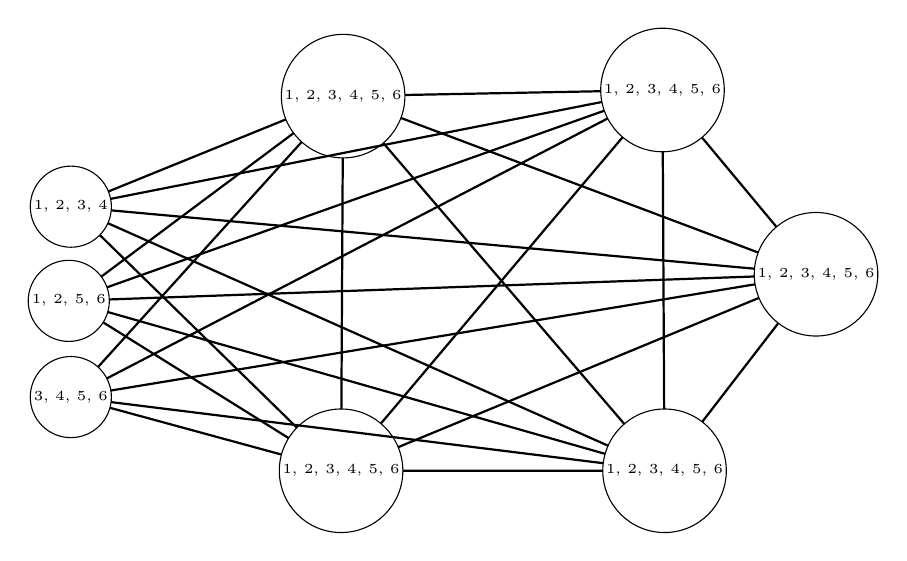
\begin{tikzpicture}[scale = 13]
\tikzstyle{VertexStyle}=[shape = circle,	
								 minimum size = 1pt,
								 inner sep = 1pt,
                         draw]
\Vertex[x = 0.312000006437302, y = 0.828000009059906, L = \tiny {1, 2, 3, 4}]{v0}
\Vertex[x = 0.310000002384186, y = 0.736000001430511, L = \tiny {1, 2, 5, 6}]{v1}
\Vertex[x = 0.312000006437302, y = 0.642000049352646, L = \tiny {3, 4, 5, 6}]{v2}
\Vertex[x = 0.889999985694885, y = 0.941999986767769, L = \tiny {1, 2, 3, 4, 5, 6}]{v3}
\Vertex[x = 0.577999949455261, y = 0.935999996960163, L = \tiny {1, 2, 3, 4, 5, 6}]{v4}
\Vertex[x = 1.03999984264374, y = 0.761999949812889, L = \tiny {1, 2, 3, 4, 5, 6}]{v5}
\Vertex[x = 0.576000034809113, y = 0.570000022649765, L = \tiny {1, 2, 3, 4, 5, 6}]{v6}
\Vertex[x = 0.891999900341034, y = 0.56999996304512, L = \tiny {1, 2, 3, 4, 5, 6}]{v7}
\Edge[](v4)(v3)
\Edge[](v5)(v3)
\Edge[](v6)(v3)
\Edge[](v7)(v3)
\Edge[](v5)(v4)
\Edge[](v6)(v4)
\Edge[](v7)(v4)
\Edge[](v5)(v7)
\Edge[](v6)(v7)
\Edge[](v6)(v5)
\Edge[](v3)(v2)
\Edge[](v4)(v2)
\Edge[](v5)(v2)
\Edge[](v6)(v2)
\Edge[](v7)(v2)
\Edge[](v3)(v0)
\Edge[](v4)(v0)
\Edge[](v5)(v0)
\Edge[](v6)(v0)
\Edge[](v7)(v0)
\Edge[](v3)(v1)
\Edge[](v4)(v1)
\Edge[](v5)(v1)
\Edge[](v6)(v1)
\Edge[](v7)(v1)
\end{tikzpicture}
\caption{A bad $d_1$-assignment on $\join{K_5}{E_3}$.}
\label{fig:K_5vE_3}
\end{figure}
% end K_5 v E_3


\begin{lem}
$\join{K_t}{E_3}$ is $d_1$-choosable iff $t \geq 6$.
\label{K_tLemma}
\end{lem}
\begin{proof}
That if $t \geq 6$, then $\join{K_t}{E_3}$ is $d_1$-choosable follows from Lemma \ref{ConnectedAtLeast6Poss}.  For the other direction it is enough to show that $\join{K_5}{E_3}$ is not $d_1$-choosable.  Figure \ref{fig:K_5vE_3} shows a bad $d_1$-assignment on $\join{K_5}{E_3}$.
\end{proof}

\begin{cor}\label{K_tClassification}
For $t \geq 4$, $\join{K_t}{B}$ is not $d_1$-choosable iff $B$ is almost complete; or $t = 4$ and $B$ is $E_3$ or a claw; or $t = 5$ and $B$ is $E_3$.
\end{cor}
\begin{lem}\label{P3Classification}
$\join{P_3}{B}$ is not $d_1$-choosable iff $B$ is $E_2$ or complete.
\end{lem}
\begin{proof}
Moving the center of $P_3$ to the other side of the join and applying Lemma
\ref{E2Classification} proves the lemma.
\end{proof}

\begin{lem}\label{AJoinP_4}\label{K3P4}
$\join{K_3}{P_4}$ is $d_1$-choosable.
\end{lem}
\begin{proof}
Suppose otherwise.  Denote the vertices of the $P_4$ as $y_1$, $y_2$, $y_3$,
$y_4$, in order.  Note that $|L(y_1)|+|L(y_3)|=4+5\ge |G|+1$ and
$|L(y_2)|+|L(y_4)|=5+4\ge |G|+1$.  Now we apply (2) of Lemma~\ref{ind-sets}
with $I_1=\{y_1,y_3\}$ and $I_2=\{y_2,y_4\}$.
\end{proof}


\begin{figure}[htb]
\centering
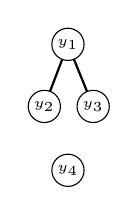
\begin{tikzpicture}[scale = 10]
\tikzstyle{VertexStyle}=[shape = circle,	
								 minimum size = 1pt,
								 inner sep = 1.2pt,
                         draw]
\Vertex[x = 0.481999963521957, y = 0.880285702645779, L = \tiny {$y_1$}]{v0}
\Vertex[x = 0.451999992132187, y = 0.801428586244583, L = \tiny {$y_2$}]{v1}
\Vertex[x = 0.513999998569489, y = 0.801428586244583, L = \tiny {$y_3$}]{v2}
\Vertex[x = 0.482000023126602, y = 0.720285713672638, L = \tiny {$y_4$}]{v3}
\Edge[](v1)(v0)
\Edge[](v2)(v0)
\end{tikzpicture}
\caption{The antipaw.}
\label{fig:antipaw}
\end{figure}

\begin{lem}\label{AntiPaw}
$\join{K_3}{\text{antipaw}}$ is $d_1$-choosable.
\end{lem}
\begin{proof}
Suppose not. We use the labeling of the antipaw given in
Figure \ref{fig:antipaw}. Since the antipaw is not a disjoint union of at most
two complete graphs, Lemma \ref{ConnectedEqual3} gives us a minimal bad
$d_1$-assignment $L$ on $\join{K_3}{\text{antipaw}}$ with $\card{Pot(L)} \leq
5$.  Note that $\card{L(y_1)} + \card{L(y_4)} \geq 6$ and $\card{L(y_2)} +
\card{L(y_3)} \geq 6$.  Hence, by Lemma \ref{IntersectionsInB}, $\card{L(y_1)
\cap L(y_4)} = 1$ and $L(y_1) \cap L(y_4) = L(y_2) \cap L(y_3)$.  But then we
have $c \in L(y_2) \cap L(y_3) \cap L(y_4)$ and after coloring $y_2, y_3$, and
$y_4$ with $c$ we can complete the coloring, getting a contradiction.
\end{proof}

\begin{lem}\label{ConnectedEqual3Poss}
\label{K3Classification}
$\join{K_3}{B}$ is not $d_1$-choosable iff
$B$ is almost complete, $\djunion{K_t}{K_{\card{B} - t}}$,
$\djunion{\djunion{K_1}{K_t}}{K_{\card{B} - t - 1}}$, $\djunion{E_3}{K_{\card{B}
- 3}}$, or $\card{B} \leq 5$ and $B = \join{E_3}{K_{\card{B} - 3}}$.
\end{lem}
\begin{proof}
Let $\join{K_3}{B}$ be a graph that is not $d_1$-choosable and let $B$ be none
of the specified graphs.  Lemma \ref{ConnectedEqual3} gives us a minimal bad
$d_1$-assignment $L$ on $\join{K_3}{B}$ with $\card{Pot(L)} \leq \card{B} + 1$.
Furthermore, the proof of Lemma~\ref{ConnectedEqual3} shows that we can color $B$ with at most $|B|-1$ colors.  
In particular we have nonadjacent $x, y \in V(B)$ and $c \in L(x) \cap L(y)$.  
Coloring $x$ and $y$ with $c$ leaves a list assignment $L'$ on $D \DefinedAs B - \set{x, y}$.  
If $c \in L'(z)$ for some $z \in V(D)$, then $\set{x, y, z}$ is independent and we can color $z$ with $c$ and complete the coloring to get a contradiction.  
Hence $Pot(L') = Pot(L) - \set{c}$.  

Suppose, for a contradiction, that $D$ is not the disjoint union of at most two
complete subgraphs.  If $\alpha(D) \geq 3$, let $J$ be a maximum independent set in
$D$ and set $\gamma \DefinedAs 0$.  Otherwise $D$ contains an induced $P_3$
$abc$ and we let $J \subseteq V(D)$ be a maximal independent set containing $\set{a,
c}$ and set $\gamma \DefinedAs 1$.  Lemma~\ref{BasicZeta} implies that
$\sum_{v\in J}d_D(v)\ge |D|-|J|+\gamma$.  Since $L$ is bad, we must have 

\begin{align*}
\sum_{v \in J} \card{L'(v)} &\leq \card{Pot(L')} \\
\sum_{v \in J} \card{L'(v)} &\leq \card{B} \\
2\card{J} + \sum_{v \in J} d_D(v) &\leq \card{B} \\
2\card{J} + \card{D} - \card{J} + \gamma &\leq \card{B} \\
\card{J} + \card{D} + \gamma &\leq \card{B} \\
\card{J} + \card{B} - 2 + \gamma &\leq \card{B}.
\end{align*}

Hence $\card{J} \leq 2 - \gamma$, a contradiction.  Therefore $D$ is indeed the
disjoint union of at most two complete subgraphs.  (Additionally, if $D$ is not
complete then $v \in V(D)$ is not adjacent to both $x$ and $y$ since then we
would get the same contradictory degree sum as in the case when $\gamma = 1$.)
We now consider the case that $D$ is a complete graph and the case that $D$ is
the disjoint union of two complete graphs.

%As we saw in the proof of Lemma \ref{ConnectedEqual3}, we have at least one nonadjacent pair $\set{x, y} \subseteq V(B)$ with $L(x) \cap L(y) \neq \emptyset$.  Put $D \DefinedAs B - \set{x, y}$.  Then $D$ is the disjoint union of at most two complete subgraphs.

First, suppose $D$ is a complete graph.  Plainly, $\card{D} \geq 2$. Put $X
\DefinedAs N(x) \cap V(D)$ and $Y \DefinedAs N(y) \cap V(D)$. Suppose $X - Y
\neq \emptyset$ and pick $z \in X - Y$.  We have $\card{L(y)} + \card{L(z)} \ge
d(y) + d(z) - 2 = d_B(y) + d_B(z) + 4 \geq 0 + \card{B} - 2 + 4 = \card{B} +
2 > \card{Pot(L)}$. By repeating the argument given above for $B-\set{x,y}$,
we see that $B - \set{y, z}$ is also the disjoint union of at most two
complete subgraphs.  In particular, $x$ is adjacent to all or none of $D - z$. 
If all, then $B$ is almost complete, if none then $B$ contains an induced $P_4$
or antipaw, and both possibilities give contradictions by Lemmas \ref{AJoinP_4}
and \ref{AntiPaw}.  Hence $X - Y = \emptyset$.  Similarly, $Y - X = \emptyset$,
so $X = Y$.  Since $B$ is not $\djunion{E_2}{K_{\card{B} - 2}}$, $\card{X} >
0$.  If $X = V(D)$, then $B$ is almost complete.  If $|V(D)-X|\ge 2$, then pick
$w_1, w_2\in V(D)-X$.  Now by considering degrees, we see that $L(x)\cap
L(w_1)$ and $L(y)\cap L(w_2)$ are both nonempty.  Now we can color $x, y, w_1,
w_2$ using only 2 colors, and then complete the coloring.  Hence, we must have
$|V(D)-X|=1$, so let $\{w\}=V(D)-X$.  Now $x$ and $y$ are joined to $D - w$ and
hence $B$ is $\join{E_3}{K_{\card{B} - 3}}$, a contradiction.

Thus $D$ must instead be the disjoint union of two complete subgraphs $D_1$ and
$D_2$.  For each $i \in \irange{2}$, put $X_i \DefinedAs N(x) \cap V(D_i)$ and
$Y_i \DefinedAs N(y) \cap V(D_i)$.  From our parenthetical remark above, we
know that $X_i \cap Y_i = \emptyset$.  Suppose we have $z_1 \in V(D_1)$ and
$z_2 \in V(D_2)$ such that $L(z_1) \cap L(z_2) \neq \emptyset$. Then, by Lemma
\ref{IntersectionsInB}, $L(z_1) \cap L(z_2) = L(x) \cap L(y)$.  Since no independent
set of size three can have a color in common, the edges $z_1x$ and $z_2y$ or
$z_1y$ and $z_2x$ must be present.
Using the same argument as for $B-\set{x,y}$, we see that $B - \set{z_1, z_2}$
is the disjoint union of at most two complete subgraphs.  
So each of $x$ and $y$ is adjacent to all or none of each of $V(D_1-z_1)$ and
$V(D_2-z_2)$.
Thus, by symmetry, we may assume that $V(D_1 - z_1) \subseteq X_1$
and $V(D_2 - z_2) \subseteq Y_2$.  If $\card{D_1} = \card{D_2} = 1$, then $B$
is the disjoint union of two cliques, a contradiction.  So, by symmetry, we may
assume that $\card{D_1} \geq 2$.  Pick $w \in V(D_1 - z_1)$. If $x$ is not
adjacent to $z_1$, then $xwz_1$ is an induced $P_3$ in $B$.  Since $X_1 \cap
Y_1 = \emptyset$, this $P_3$ together with $y$ either induces a $P_4$ or an
antipaw, contradicting Lemmas \ref{AJoinP_4} and \ref{AntiPaw}.  Hence $X_1 =
V(D_1)$.  Similarly, if $\card{D_2} \geq 2$, then $Y_2 = V(D_2)$ and $B$ is the
disjoint union of two complete subgraphs, a contradiction.  Hence $D_2 =
\set{z_2}$.  But $z_2$ must be adjacent to $y$, so $B$ is again the disjoint
union of two cliques, a contradiction.

Thus for every $z_1 \in V(D_1)$ and $z_2 \in V(D_2)$ we have $L(z_1) \cap L(z_2) = \emptyset$. 
%Suppose we have, for each $i \in \irange{2}$, $z_i \in X_i \cup Y_i$.  
Suppose there exist $z_1\in V(D_1)$ and $z_2\in V(D_2)$ such that $z_1$ and
$z_2$ are each adjacent to at least one of $x$ and $y$.
Then $\card{L(z_1)} + \card{L(z_2)} \geq d(z_1) + d(z_2) - 2 \geq d_B(z_1) + d_B(z_2) + 4 \geq \card{B} - 4 + 2 + 4 = \card{B} + 2 > \card{Pot(L)}$.  Hence $L(z_1) \cap L(z_2) \neq \emptyset$, a contradiction.

Thus, by symmetry, we may assume that there are no edges between $D_1$ and $\set{x, y}$.  Since no vertex in $D_2$ is adjacent to both $x$ and $y$, only one of $x$ or $y$ can have neighbors in $D_2$ lest $B$ contain an induced $P_4$ contradicting Lemma \ref{AJoinP_4}. Without loss of generality, we may assume that $y$ has no neighbors in $D_2$. Pick $w \in D_1$ and $z \in V(D_2)$.  

Suppose that $|D_1|\ge 2$, $|D_2|\ge 2$, and there exists $t\in D_2$ such that
$x$ and $t$ are nonadjacent.  Now choose $u,v\in V(D_1)$ and $w\in
V(D_2)\setminus\{t\}$.  
Now $\set{v, w, y}$ is independent and $\card{L(v)} + \card{L(w)} + \card{L(y}) \geq d(v) + d(w) + d(y) - 3 \geq d_B(v) + d_B(w) + d_B(y) + 6 \geq \card{B} + 2 > \card{Pot(L)}$. Hence either $L(v) \cap L(y) \neq \emptyset$ or $L(w) \cap L(y) \neq \emptyset$.  
Similarly, either $L(u)\cap L(x) \neq \emptyset$ or $L(t)\cap L(x)\neq
\emptyset$.  Thus, we can color 4 vertices using only 2 colors, and we can
complete the coloring.
So now either $|D_1|=1$, $|D_2|=1$, or $D_2\subset N(x)$.

If $|D_2|=1$, then either $B=K_1+K_2+K_{|B|-3}$ or else $B=E_3+K_{|B|-3}$, both
of which are forbidden.  Similarly, if $|D_1|=1$ and $x$ is adjacent to all or
none of $D_2$, then $B=K_1+K_1+K_{|B|-2}$ or $E_3+K_{|B|-3}$.
Finally, if $x$ is adjacent to some, but not all of $D_2$, then $B$ contains an
antipaw.  By Lemma~\ref{AntiPaw}, this is a contradiction.
%In the former case, we must have $V(D_2) = \set{z}$ and hence $B$ is either $\djunion{E_3}{K_{\card{B} - 3}}$ or $\djunion{\overline{P_3}}{K_{\card{B} - 3}}$, a contradiction.  In the latter case, either $V(D_1) = \set{w}$ and $x$ hits all or none of $D_2$; or $x$ hits all of $D_2$.  In all cases, $B$ is one of the graphs we have excluded.  This final contradiction completes the proof.

It remains to show that $\join{K_3}{B}$ is not $d_1$-choosable for any of the
specified $B$'s.  For $B$ almost complete, this follows from Lemma
\ref{AlmostCompleteGraphsNotD1} and for $\join{E_3}{K_{\card{B} - 3}}$, from
Lemma \ref{K_tClassification}.  For all the rest of the options we will give a
bad list assignment with lists $\irange{\card{B}+1}$ on the $K_3$.
Suppose $\djunion{K_t}{K_{\card{B} - t}}$.  On the $K_t$ the lists $\irange{t +
1}$ and on the $K_{\card{B} - t}$ the lists $\irange{\card{B} + 1} \smallsetminus \irange{t}$.  Then any coloring of $\join{K_3}{B}$ from the lists
must use three colors on the $K_3$ and hence at least one of the cliques
loses at least two colors leaving it uncolorable.  Now
suppose $B = \djunion{\djunion{K_1}{K_t}}{K_{\card{B} - t - 1}}$.  Use
the list $\set{1, \card{B} + 1}$ on the $K_1$, the lists $\irange{t +
1}$ on the $K_t$ and the lists $\irange{\card{B + 1}}
\smallsetminus \irange{t + 1}$ on the $K_{\card{B} - t - 1}$.  This list
assignment is clearly bad on $\join{K_3}{B}$.  

Finally suppose $B = \djunion{E_3}{K_{\card{B} - 3}}$.  Give the three $K_1$'s the lists
$\set{1,2}$, $\set{1,3}$, $\set{2,3}$ and the $K_{\card{B} - 3}$ the list
$\irange{\card{B} + 1} \smallsetminus \irange{3}$.  Again, this is clearly a bad
list assignment on $\join{K_3}{B}$.
\end{proof}


%We'll use the following simple facts a few times, so we pull them out into  lemmas.

%\begin{lem}\label{independent3MustHaveSomePairs}
%Let $S_1, \ldots, S_m, R$ be nonempty finite sets such that $S_i \cap S_j \cap S_k = \emptyset$ for all $1 \leq i < j < k \leq m$ and $S_i \cap S_j \in \set{\emptyset, R}$ for each $1 \leq i < j \leq m$.  Then $\sum_{i \in \irange{m}} \card{S_i} \leq \card{\bigcup_{i \in \irange{m}} S_i} + \card{R}$.
%\end{lem}
%\begin{proof}
%Since $S_i \cap S_j \cap S_k = \emptyset$ for all $1 \leq i < j < k \leq m$, at most one of the $S_i \cap S_j$ can be nonempty. Hence, by the inclusion-exclusion principle, we have $\card{\bigcup_{i \in \irange{m}} S_i} = \sum_{i \in \irange{m}} \card{S_i} - \sum_{1 \leq i < j \leq m} \card{S_i \cap S_j} \geq \sum_{i \in \irange{m}} \card{S_i} - \card{R}$.
%\end{proof}

%\begin{lem}\label{TwoAndThreeindependent}
%Let $A$ be a graph with $\card{A} \geq 2$ and $B$ an arbitrary graph.
%Let $L$ be a $d_1$-assignment on $G \DefinedAs \join{A}{B}$. If $B$ has disjoint independent sets $\set{x_1, x_2}$ and $\set{y_1, \ldots, y_m}$ such that $L(x_1) \cap L(x_2) \neq \emptyset$ (in particular, if $d_G(x_1) + d_G(x_2) \geq \card{Pot(L)} + 3$) and $\sum_{i \in \irange{m}} d_G(y_i) \geq \card{Pot(L)} + m + 2$, then $L$ is good on $\join{A}{B}$.
%\end{lem}
%\begin{proof}
%Assume $B$ has disjoint independent sets $\set{x_1, x_2}$ and $\set{y_1, \ldots, y_m}$ such that $L(x_1) \cap L(x_2) \neq \emptyset$ and $\sum_{i \in \irange{m}} d_G(y_i) \geq \card{Pot(L)} + m + 2$.

%Suppose $L$ is bad on $\join{A}{B}$. Then by Lemma \ref{IntersectionsInB}, for $1 \leq i < j \leq m$ we have $L(y_i) \cap L(y_j) = \emptyset$ or $\card{L(x_1) \cap L(x_2)} = 1$ and $L(y_i) \cap L(y_j) = L(x_1) \cap L(x_2)$.  By Lemma \ref{independent3MustHaveSomePairs}, $\sum_{i \in \irange{m}} \card{L(y_i)} \leq \card{Pot(L)} + 1$ and hence $\sum_{i \in \irange{m}} d_G(y_i) \leq \card{Pot(L)} + m + 1$, a contradiction.
%\end{proof}

\begin{lem}
$\join{K_2}{P_5}$ is $d_1$-choosable.
\label{P_5*K_2}
\end{lem}
\begin{proof}
Suppose otherwise. By Lemma \ref{ConnectedIsK2}, we have a minimal bad
$d_1$-assignment $L$ on $\join{P_5}{K_2}$ with $\card{Pot(L)} \leq 5$.  Let
$y_1, y_2, y_3, y_4, y_5$ denote the vertices of the $P_5$ in order.  Now
$|L(y_2)|+|L(y_4)|\ge 6 \ge |Pot(L)|+1$ and $|L(y_1)|+|L(y_3)|+|L(y_5)|\ge 7
\ge |Pot(L)|+2$.  So $\set{y_2, y_4}$ and $\set{y_1, y_3, y_5}$ satisfy the
hypotheses of Lemma \ref{ind-sets}, giving a contradiction.
\end{proof}

\begin{figure}[htb]
\centering
\subfloat[The chair.]{\label{fig:chair}
{\parbox{2.5cm}{
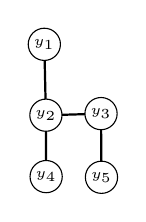
\begin{tikzpicture}[scale = 10]
\tikzstyle{VertexStyle}=[shape = circle,	
								 minimum size = 1pt,
								 inner sep = 1.2pt,
                         draw]
\Vertex[x = 0.236114323139191, y = 0.890571415424347, L = \tiny {$y_1$}]{v0}
\Vertex[x = 0.238114297389984, y = 0.800571441650391, L = \tiny {$y_2$}]{v1}
\Vertex[x = 0.308114320039749, y = 0.802571445703506, L = \tiny {$y_3$}]{v2}
\Vertex[x = 0.238400012254715, y = 0.722571432590485, L = \tiny {$y_4$}]{v3}
\Vertex[x = 0.308685749769211, y = 0.721714287996292, L = \tiny {$y_5$}]{v4}
\Edge[](v1)(v0)
\Edge[](v1)(v3)
\Edge[](v1)(v2)
\Edge[](v4)(v2)
\end{tikzpicture}}}}\qquad\qquad
\subfloat[The antichair.]{\label{fig:antichair}
{\parbox{3cm}{
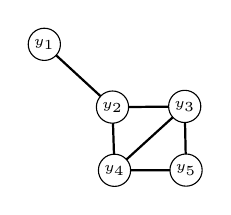
\begin{tikzpicture}[scale = 10]
\tikzstyle{VertexStyle}=[shape = circle,	
								 minimum size = 1pt,
								 inner sep = 1.2pt,
                         draw]
\Vertex[x = 0.151542887091637, y = 0.880285702645779, L = \tiny {$y_1$}]{v0}
\Vertex[x = 0.238114297389984, y = 0.800571441650391, L = \tiny {$y_2$}]{v1}
\Vertex[x = 0.32982861995697, y = 0.801428586244583, L = \tiny {$y_3$}]{v2}
\Vertex[x = 0.240685701370239, y = 0.720285713672638, L = \tiny {$y_4$}]{v3}
\Vertex[x = 0.331542909145355, y = 0.720571428537369, L = \tiny {$y_5$}]{v4}
\Edge[](v1)(v0)
\Edge[](v1)(v3)
\Edge[](v1)(v2)
\Edge[](v4)(v2)
\Edge[](v4)(v3)
\Edge[](v3)(v2)
\end{tikzpicture}}}}
\caption{Labelings of the chair and the antichair.}
\end{figure}



\begin{lem}
$\join{K_2}{\text{chair}}$ is $d_1$-choosable.
\label{chair*K_2}
\end{lem}
\begin{proof}
Suppose otherwise. We use the labeling of the chair given in Figure
\ref{fig:chair}.  Since the chair has an induced claw, Lemma \ref{ConnectedIsK2}
gives us a minimal bad $d_1$-assignment $L$ on $\join{K_2}{\text{chair}}$ with
$\card{Pot(L)} \leq 5$.  Now $|L(y_2)|+|L(y_5)|\ge 6 \ge |Pot(L)|+1$ and
$|L(y_1)|+|L(y_3)|+|L(y_4)|\ge 7 \ge |Pot(L)|+2$.  Then $\set{y_2, y_5}$ and
$\set{y_1, y_3, y_4}$ satisfy the hypotheses of Lemma \ref{ind-sets}, giving a
contradiction.
\end{proof}

\begin{lem}
$\join{K_2}{\text{antichair}}$ is $d_1$-choosable.
\label{antichair*K_2}\label{K2Antichair}
\end{lem}
\begin{proof}
Suppose otherwise. We use the labeling of the antichair given in Figure
\ref{fig:antichair}.  Since the antichair has an induced $K_4^-$, Lemma
\ref{ConnectedIsK2} gives us a minimal bad $d_1$-assignment $L$ on
$\join{K_2}{\text{antichair}}$ with $\card{Pot(L)} \leq 5$. We have $\card{L(y_2)} + \card{L(y_5)} \geq 7$ and hence $\card{L(y_2) \cap L(y_5)} \geq 2$.  But then, by Lemma \ref{IntersectionsInB}, we have the contradiction $\card{L(y_1)} + \card{L(y_3)} \leq 5$.
\end{proof}

\begin{lem}
$\join{K_2}{C_5}$ is $d_1$-choosable.
\label{C_5*K_2}
\end{lem}
\begin{proof}
Suppose otherwise. By the Small Pot Lemma, we have a minimal bad
$d_1$-assignment $L$ on $\join{C_5}{K_2}$ with $\card{Pot(L)} \leq 6$.  Let
$y_0, y_1, y_2, y_3, y_4, y_0$ denote in order the vertices of the $C_5$.  Then for $0 \leq i < j \leq 4$ with $i - j \not \equiv 1 (\text{mod }5)$ we have $\card{L(y_i)} + \card{L(y_j)} \geq d(y_i) + d(y_j) - 2 = 6$.

First suppose $\card{Pot(L)} \leq 5$.  Then each nonadjacent pair has a color in
common and by applying Lemma \ref{IntersectionsInB} multiple times we see that
there must exist $c \in \bigcap_{0 \leq i \leq 4} L(y_i)$ and no nonadacent
pair can have a color other than $c$ in common.  Put $S_i = L(y_i) - \set{c}$
and $T = Pot(L) - \set{c}$.  Then we must have $S_0 = T - S_3$, $S_1 = T - S_3
= T - S_4$ and $S_2 = T - S_4$.  Hence $S_0 = S_1 = S_2$ contradicting $S_0
\cap S_2 = \emptyset$.

Therefore we must have $\card{Pot(L)} = 6$.  Thus for nonadjacent $y_i$ and $y_j$, $L(y_i) = Pot(L) - L(y_j)$.  We have $L(y_0) = Pot(L) - L(y_3)$, $L(y_1) = Pot(L) - L(y_3) = Pot(L) - L(y_4)$ and $L(y_2) = Pot(L) - L(y_4)$.  Hence $L(y_0) = L(y_1) = L(y_2)$.  Thus we may color $y_0$ and $y_2$ the same and complete this coloring to the rest of $B$ contradicting Lemma \ref{ConnectedPot}.
\end{proof}

\begin{figure}[htb]
\centering
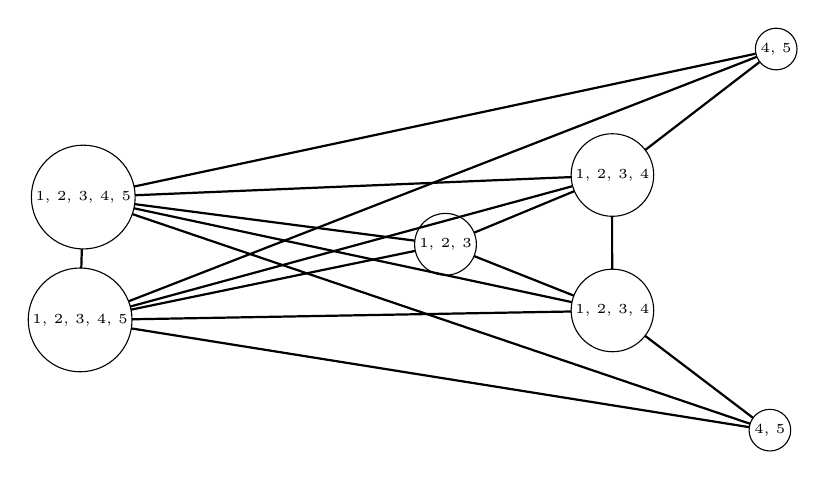
\begin{tikzpicture}[scale = 20]
\tikzstyle{VertexStyle}=[shape = circle,	
								 minimum size = 1pt,
								 inner sep = 1.2pt,
                         draw]
\Vertex[x = 0.436000019311905, y = 0.793999999761581, L = \tiny {1, 2, 3}]{v0}
\Vertex[x = 0.541999936103821, y = 0.838000014424324, L = \tiny {1, 2, 3, 4}]{v1}
\Vertex[x = 0.54200005531311, y = 0.752000018954277, L = \tiny {1, 2, 3, 4}]{v2}
\Vertex[x = 0.6460000872612, y = 0.918000027537346, L = \tiny {4, 5}]{v3}
\Vertex[x = 0.642000019550323, y = 0.675999999046326, L = \tiny {4, 5}]{v4}
\Vertex[x = 0.20600001513958, y = 0.823999986052513, L = \tiny {1, 2, 3, 4, 5}]{v5}
\Vertex[x = 0.204000011086464, y = 0.745999991893768, L = \tiny {1, 2, 3, 4, 5}]{v6}
\Edge[](v1)(v0)
\Edge[](v2)(v0)
\Edge[](v1)(v2)
\Edge[](v3)(v1)
\Edge[](v4)(v2)
\Edge[](v6)(v5)
\Edge[](v0)(v6)
\Edge[](v1)(v6)
\Edge[](v2)(v6)
\Edge[](v3)(v6)
\Edge[](v4)(v6)
\Edge[](v0)(v5)
\Edge[](v1)(v5)
\Edge[](v2)(v5)
\Edge[](v3)(v5)
\Edge[](v4)(v5)
\end{tikzpicture}
\caption{A bad $d_1$-assignment on $\join{\text{bull}}{K_2}$.}
\label{fig:bullvK_2}
\end{figure}

\begin{lem}
$\join{K_2}{2P_3}$ is $d_1$-choosable.
\label{2P_3*K_2}
\end{lem}
\begin{proof}
Suppose otherwise. Let $y_1, y_2, y_3$ and $y_4, y_5, y_6$ denote in order the
vertices of the two $P_3$'s.  Lemma \ref{ConnectedIsK2} gives us a minimal bad
$d_1$-assignment $L$ on $\join{K_2}{2P_3}$ with $\card{Pot(L)} \leq 6$.  

Since $|L(y_1)|+|L(y_3)|+|L(y_4)|+|L(y_6)|=8\ge |Pot(L)|+2$, either three of
these vertices share a common color, or else two pairs of them share distinct
common colors.
Thus, if $L(y_2) \cap L(y_5) \neq \emptyset$, then we can color $G$ by
Lemma~\ref{IntersectionsInB}.  Hence $L(y_2)\cap L(y_5)=\emptyset$.

By summing list sizes, we see that some pair among each of $\set{y_1, y_3,
y_5}$ and $\set{y_2, y_4, y_6}$ must have a color in common.  Since there are
no edges between $\set{y_1, y_3}$ and $\set{y_4, y_6}$, if $L(y_1) \cap L(y_3)
\neq \emptyset$ and $L(y_4) \cap L(y_6) \neq \emptyset$, then we get a
contradiction.
 By symmetry, we may assume that the other two options are either $L(y_1) \cap
L(y_3) \neq \emptyset$ and $L(y_2) \cap L(y_4) \neq \emptyset$ or else $L(y_1)
\cap L(y_5) \neq \emptyset$ and $L(y_2) \cap L(y_4) \neq \emptyset$.  In the
former case, by Lemma \ref{IntersectionsInB},we must have $L(y_1) \cap L(y_3)
\cap L(y_4) \neq \emptyset$, a contradiction.  In the latter case, $L(y_1) \cap
L(y_5) \neq L(y_2) \cap L(y_4)$ since $L(y_2) \cap L(y_5) = \emptyset$,
contradicting Lemma \ref{IntersectionsInB}.  \end{proof}

\begin{figure}[htb]
\centering
\subfloat[The anticlaw.]{\label{fig:anticlaw}
{\parbox{3.5cm}{
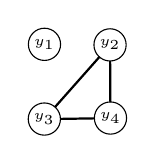
\begin{tikzpicture}[scale = 10]
\tikzstyle{VertexStyle}=[shape = circle,	
								 minimum size = 1pt,
								 inner sep = 1.2pt,
                         draw]
\Vertex[x = 0.131151512265205, y = 0.944127283990383, L = \tiny {$y_1$}]{v0}
\Vertex[x = 0.214424252510071, y = 0.943400021642447, L = \tiny {$y_2$}]{v1}
\Vertex[x = 0.13096971809864, y = 0.849218189716339, L = \tiny {$y_3$}]{v2}
\Vertex[x = 0.214969739317894, y = 0.850490942597389, L = \tiny {$y_4$}]{v3}
\Edge[](v2)(v3)
\Edge[](v2)(v1)
\Edge[](v3)(v1)
\end{tikzpicture}}}}\qquad\qquad
\subfloat[The antidiamond.]{\label{fig:antidiamond}
{\parbox{3.5cm}{
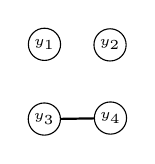
\begin{tikzpicture}[scale = 10]
\tikzstyle{VertexStyle}=[shape = circle,	
								 minimum size = 1pt,
								 inner sep = 1.2pt,
                         draw]
\Vertex[x = 0.131151512265205, y = 0.944127283990383, L = \tiny {$y_1$}]{v0}
\Vertex[x = 0.214424252510071, y = 0.943400021642447, L = \tiny {$y_2$}]{v1}
\Vertex[x = 0.13096971809864, y = 0.849218189716339, L = \tiny {$y_3$}]{v2}
\Vertex[x = 0.214969739317894, y = 0.850490942597389, L = \tiny {$y_4$}]{v3}
\Edge[](v2)(v3)
\end{tikzpicture}}}}
\caption{Labelings of the anticlaw and the antidiamond.}
\end{figure}


Note that if $L$ is a bad $d_1$ assignment on $\join{E_3}{B}$ where the $E_3$ is $\set{x_1, x_2, x_3}$, then $L(x_1) \cap L(x_2) \cap L(x_3) = \emptyset$.
\begin{lem}\label{E3JoinAntiClaw}
$\join{E_3}{\text{anticlaw}}$ is $d_1$-choosable.
\end{lem}
\begin{proof}\
Suppose otherwise. The Small Pot Lemma gives us a minimal bad $d_1$-assignment
$L$ on $\join{E_3}{\text{anticlaw}}$ with $\card{Pot(L)} \leq 6$.  Let the $E_3$
have vertices $x_1, x_2, x_3$, and let the anticlaw have vertices $y_1,
y_2, y_3, y_4$, with $y_2, y_3, y_4$ mutually adjacent.  Then $\sum_i \card{L(x_i)} = 9$ and hence there are three colors $c_1, c_2, c_3$ such that for each $t \in \irange{3}$, $c_t \in L(x_i) \cap L(x_j)$ for some $1 \leq i < j \leq 3$.  

Suppose there exists $i\in\{2,3,4\}$, say $i=2$, such that $y_1$ and $y_i$ have
a common color $c$.  We use $c$ on $y_1$ and $y_2$, and let $L'(v)=L(v)-c$ for
each uncolored $v$; note that $c$ must be absent from some $x_i$, say $x_1$. 
Now since $|L'(x_2)|+|L'(x_3)|\ge 4$, we can color $x_2$ and $x_3$
such that at least two colors remain available on $y_3$.  Finally, we greedily
color $y_4$, $y_3$, $x_3$.

Otherwise, since $\card{Pot(L)}\le 6$, we may assume that
$L(y_1)=\{a,b\}$ and $L(y_2)=L(y_3)=L(y_4)=\{c,d,e,f\}$.  Now we can color
$x_1$, $x_2$, and $x_3$ using only two colors, exactly one of which is in
$\{a,b\}$.  Finally, we greedily color $y_1, y_2, y_3$, $y_4$.
%
%
%Since $\card{L(v_1)} = 2$, some $c_t \not \in L(v_1)$.  By symmetry we may assume that $c_1 \in L(x_1) \cap L(x_2)$ and $c_1 \not \in L(v_1)$.  Since $L(x_1) \cap L(x_2) \cap L(x_3) = \emptyset$, we have $L(x_3) = \set{c_4, c_5, c_6}$ where $\set{c_4, c_5, c_6} \subseteq Pot(L) - \set{c_1}$.
%
%Now, color $x_1$ and $x_2$ with $c_1$.  Then $L(v_2) = L(v_3) = L(v_4) = \set{c_1, c_4, c_5, c_6}$ since otherwise we can color $x_3$ with the appropriate color and easily complete the coloring.
%
%Now, since $L(x_1) \cap L(x_2) \cap L(x_3) = \emptyset$ we must have $\card{Pot(L)} \geq 5$ by Lemma \ref{BasicFiniteSets}.  Hence we have $c_7 \in Pot(L) - \set{c_1, c_4, c_5, c_6}$.  By Lemma \ref{CannotColorSelfWithSelf}, $c_7 \in L(v_0)$ and $c_7 \in L(x_1) \cup L(x_2)$.  If $c_7 \in L(x_1) \cap L(x_2)$, then after coloring $x_1$ and $x_2$ with $c_7$, there is some color we can give $x_3$ such that we can complete the coloring.  By symmetry we may assume that $c_7 \in L(x_1) - L(x_2)$.
%
%Suppose $\card{Pot(L)} = 6$.  Then we have $c_8 \in Pot(L) - \set{c_1, c_4, c_5, c_6, c_7}$.  As above  $c_8 \not \in L(x_1) \cap L(x_2)$.  By Lemma \ref{CannotColorSelfWithSelf}, $c_8 \in L(v_0)$ and $c_8 \in L(x_1) \cup L(x_2)$.  Using Lemma \ref{CannotColorSelfWithSelf} again shows that $c_8 \not \in L(x_1)$.  Hence $c_8 \in L(x_2) - L(x_1)$.  So, $\set{1, 7} \subseteq L(x_1)$ and $\set{1, 8} \subseteq L(x_2)$.  By symmetry, we may assume that $c_4 \in L(x_1)$.  Now we get a contradiction by coloring $v_2, v_3$ and $v_4$ with $c_1, c_5$ and $c_6$, $x_1$ and $x_3$ with $c_4$, $x_2$ with $c_8$ and $v_0$ with $c_7$.
%
%Hence $\card{Pot(L)} = 5$.  Since $c_1 \not \in L(v_0)$, the only options for its other color are $c_4, c_5$ and $c_6$.  By symmetry, we may assume $L(v_0) = \set{c_4, c_7}$.  Now $L(x_2)$ contains one of $c_5$ or $c_6$, and these are symmetric as well so we may assume $c_6 \in L(x_2)$.  Coloring $v_2, v_3$ and $v_4$ with $c_1, c_4$ and $c_5$, $x_2$ and $x_3$ with $c_6$, $x_1$ with $c_7$ and $v_0$ with $c_4$ gives the final contradiction.
\end{proof}

\begin{lem}\label{E3Join2K2}
$\join{E_3}{2K_2}$ is $d_1$-choosable.
\end{lem}
\begin{proof}
Suppose otherwise.  The Small Pot Lemma gives us a minimal bad $d_1$-assignment
$L$ on $\join{E_3}{2K_2}$ with $\card{Pot(L)} \leq 6$.  Let the $E_3$ have
vertices $x_1, x_2$, $x_3$, and let the $2K_2$ have vertices $y_1$ adjacent
to $y_2$ and $y_3$ adjacent to $y_4$.  Then $\sum_i \card{L(x_i)} = 9$ and
hence there are three colors $c_1, c_2, c_3$ such that for each $t \in
\irange{3}$, $c_t \in L(x_i) \cap L(x_j)$ for some $1 \leq i < j \leq 3$.  If
all three $c_t$ appear on all four $y_i$, then we can 2-color the $2K_2$, and
extend the coloring to the $E_3$.  So we may assume instead without loss of
generality that $c_1$ appears on $x_1$ and $x_2$, but not $y_1$.  Now use $c_1$
on $x_1$ and $x_2$, then color greedily in the order $y_3$, $y_4$, $x_3$,
$y_2$, $y_1$.
\end{proof}
\begin{lem}\label{E3JoinE4}
$\join{E_3}{E_4}$ is $d_1$-choosable.
\end{lem}
\begin{proof}
Suppose otherwise.
Let the $E_3$ have vertices $x_1$, $x_2$, $x_3$ and let the $E_4$ have
vertices $y_1$, $y_2$, $y_3$, $y_4$.  If there exists $c\in
\cap_{i=1}^3L(x_i)$, then we use $c$ on all $x_i$ and we can finish the
coloring, so assume not.  By the Small Pot Lemma, $|Pot(L)|\le 6$, so there
exist two $y_i$, say $y_1$ and $y_2$, with a common color $c$; use $c$ on $y_1$
and $y_2$.  Now there exists some $x_i$, say $x_3$, with $c\notin L(x_i)$.  The
4-cycle induced by $x_1$, $x_2$, $y_3$, and $y_4$ is 2-choosable; then we can
extend the coloring to $x_3$.
\end{proof}

\begin{lem}\label{E3JoinAntiDiamond}
$\join{E_3}{\text{antidiamond}}$ is $d_1$-choosable.
\end{lem}
\begin{proof}
Suppose otherwise.  The Small Pot Lemma gives us a minimal bad $d_1$-assignment
$L$ on $\join{E_3}{\text{antidiamond}}$ with $\card{Pot(L)} \leq 6$.  Let the
$E_3$ have vertices $x_1, x_2$, $x_3$, and let the $\text{antidiamond}$ have
vertices $y_1$, $y_2$, $y_3$, $y_4$, with $y_3$ adjacent to $y_4$.  We can
assume tht $\cap_{i=1}^3L(x_i)=\emptyset$ (since otherwise we use a common color
on the $x_i$ and then greedily complete the coloring).  If $y_3$ or
$y_4$ has a common color $c$ with $y_1$ or $y_2$, then we can use $c$ on those
two vertices and proceed as in the case of $\join{E_3}{E_4}$, so assume not.
Again $\sum_i \card{L(x_i)} = 9$ and hence there are three colors $c_1, c_2,
c_3$ such that for each $t \in \irange{3}$, $c_t \in L(x_i) \cap L(x_j)$ for
some $1 \leq i < j \leq 3$.  So assume that $c_1$ appears on $x_1$ and $x_2$,
and use it there.  If $c_1$ appears on neither $y_1$ or $y_2$, then we greedily
color in the order $y_3$, $y_4$, $x_3$, $y_1$, $y_2$.  Otherwise $c_1$ appears
on neither $y_3$ or $y_4$, so we greedily color in the order $y_1$, $y_2$,
$x_3$, $y_3$, $y_4$.
\end{proof}

\begin{lem}\label{E3Classification}
$\join{E_3}{B}$ is not $d_1$-choosable iff $B \in \set{K_1,K_2,E_2,E_3,\overline{P_3},K_3,K_4,K_5}$.
\end{lem}
\begin{proof}
Suppose we have $B$ such that $\join{E_3}{B}$ is not $d_1$-choosable. By Lemma \ref{E2Classification}, $B$ is the disjoint union of complete subgraphs and at most one $P_3$.  If $B$ contained a $P_3$, then moving its middle vertex to the other side of the join would violate Lemma \ref{ConnectedIncompleteAtLeast4}.  By Lemma \ref{E3JoinE4}, $B$ has at most three components.  By Lemma \ref{E3JoinAntiDiamond}, if $B$ has three components, then $B = E_3$.  By Lemma \ref{E3Join2K2} and Lemma \ref{E3JoinAntiClaw}, if $B$ has two components then $B = E_2$ or $B = \overline{P_3}$.  Otherwise $B$ is complete and Lemma~\ref{K_tLemma}
%\ref{ConnectedAtLeast6Poss} 
shows that $\card{B} \leq 5$.  This proves the forward implication.

For the other direction, it is easy to verify that $\join{E_3}{B}$ is not
$d_1$-choosable for the listed graphs.  The cases $B\in \{K_1,K_2,E_2\}$ are
nearly trivial.  For $B=E_3$, we are simply recalling that $K_{3,3}$ is not
2-choosable.  For $B\in\{K_3,K_4,K_5\}$, see Figure~\ref{fig:K_5vE_3}.  Finally,
suppose that $B=\overline{P_3}$.  Let $x_1$, $x_2$, $x_3$ denote the vertices of
the $E_3$ and let $y_1$, $y_2$, $y_3$ denote the vertices of the
$\overline{P_3}$, where $y_2$ and $y_3$ are adjacent.  Assign the lists
$L(x_1)=\{1,2\}$, $L(x_2)=\{1,3\}$, $L(x_3)=\{2,3\}$, $L(y_1)=\{1,2\}$, and
$L(y_2)=L(y_3)=\{1,2,3\}$.  To color the $\overline{P_3}$, we clearly use at
least two colors, but now some vertex of the $E_3$ has no remaining colors.
\end{proof}

\begin{lem}\label{AntiP3Join2K2}
$\join{\overline{P_3}}{2K_2}$ is $d_1$-choosable.
\end{lem}
\begin{proof}
Let $x_1$, $x_2$, $x_3$ be the vertices of $\overline{P_3}$, with $x_2$ adjacent
to $x_3$, and let $y_1$, $y_2$, $y_3$, $y_4$ be the vertices of $2K_2$, with
$y_1$ adjacent to $y_2$ and $y_3$ adjacent to $y_4$.  By the Small Pot Lemma,
$|Pot(L)|\le 6$, so $x_1$ and $x_2$ have a common color $c_1$.  If $c_1$ is
absent from the list of some $y_i$, say $y_1$, then we can use $c_1$ on $x_1$
and $x_2$, then greedily color in the order $y_4$, $y_3$, $x_3$, $y_2$, $y_1$.
Hence $c_1$ appears on all $y_i$.  If $|Pot(L)|\le 5$, then $x_1$ and $x_2$ have
a second common color $c_2$.  Since $c_1$ and $c_2$ must appear on all $y_i$, we
can 2-color the $2K_2$, then greedily color $x_1$, $x_2$, and $x_3$.  So we can
conclude that $L(x_1)\cap L(x_2)=c_1$ and $L(x_1)\cap L(x_3)=c_1$.  Similarly,
we can 2-color the $2K_2$ if $y_1$ and $y_3$ have any common color other than $c_1$.

Now we use $c_1$ on $y_2$ and $y_4$, and let $L'(v)=L(v)-c_1$ for all uncolored
$v$.  Now $|Pot(L')|=|Pot(L)|-1=5$. Let $S=\{x_1,x_2,x_3,y_1,y_3\}$.  To show
that we can finish the coloring, we use Hall's Theorem.  We only need to
consider subsets $T\subset S$ of size 3 or 4.  If $|T|=3$, then either
$\{y_1,y_3\}\subset T$, so $|\cup_{v\in T}L'(v)|\ge |L'(y_1)|+|L'(y_3)|\ge 4$,
or else $T$ contains $x_2$ or $x_3$.  Since $|L'(x_2)|=|L'(x_3)|=3$, we are
done.  If $|T|=4$, then either $\{y_1,y_3\}\subset T$ or $\{x_1,x_2\}\subset T$
or  $\{x_1,x_3\}\subset T$.  In each case $|\cup_{v\in T}L'(v)|\ge 4$.
\end{proof}

\begin{lem}\label{AntiP3JoinAntiDiamond}
$\join{\overline{P_3}}{\text{antidiamond}}$ is $d_1$-choosable.
\end{lem}
\begin{proof}
Let $x_1$, $x_2$, $x_3$ be the vertices of $\overline{P_3}$, with $x_2$ adjacent
to $x_3$, and let $y_1$, $y_2$, $y_3$, $y_4$ be the vertices of the
$\text{antidiamond}$, with $y_3$ adjacent to $y_4$.  By the Small Pot Lemma,
$|Pot(L)|\le 6$, so $x_1$ and $x_2$ have a common color $c$.   If $c$ is absent
from $y_4$, then we use $c$ on $x_1$ and $x_2$, then greedily color $y_1$,
$y_2$, $x_3$, $y_3$, $y_4$.  Similarly, if $c$ is absent from $y_1$ and $y_2$,
then we use $c$ on $x_1$ and $x_2$, then greedily color $y_3$, $y_4$, $x_3$,
$y_2$, $y_1$.  So $c$ must appear on $y_1$ (or $y_2$) and $y_3$, and we use it
there.  Let $L'(v)=L(v)-c$ for all uncolored vertices.  Now if there exists
$c_2\in L'(y_2)\setminus L'(x_2)$, then we can use $c_2$ on $y_2$ and greedily
color $x_1$, $y_4$, $x_3$, $x_2$.  The same argument holds if there exists
$c_2\in L'(y_4)\setminus L'(x_2)$.  Thus, we must have $(L'(y_2)\cup
L'(y_4))\subseteq L'(x_2)$, so $y_2$ and $y_4$ have a common color $c_2$.  We
use it on them and greedily color $x_1$, $x_2$, $x_3$.
\end{proof}

\begin{lem}\label{E4JoinAntiP3}
$\join{\overline{P_3}}{E_4}$ is $d_1$-choosable.
\end{lem}
\begin{proof}
Let $x_1$, $x_2$, $x_3$ be the vertices of $\overline{P_3}$, with $x_2$ adjacent
to $x_3$, and let $y_1$, $y_2$, $y_3$, $y_4$ be the vertices of $E_4$.  If three
of the $y_i$'s (say $y_1$, $y_2$, and $y_3$) have a common color $c$, then use
$c$ on them, and now greedily color in the order $y_4$, $x_1$, $x_2$, $x_3$.  By
the Small Pot Lemma, $x_1$ and $x_2$ have a common color $c$, which we use on
them.  Now $c$ appears on at most two $y_i$, say $y_1$ and $y_2$, so we can
greedily color in the order $y_1$, $y_2$, $x_3$, $y_3$, $y_4$.
\end{proof}

\begin{lem}\label{AntiP3Classification}
$\join{\overline{P_3}}{B}$ is not $d_1$-choosable iff $B$ is $E_3$,
$K_{\card{B}}$, or $\djunion{K_1}{K_{\card{B} - 1}}$.
\end{lem}
\begin{proof}
Since $\overline{P_3}$ contains an $E_2$, Lemma \ref{E2Classification} shows that $B$ is the disjoint union of complete subgraphs and at most one $P_3$.  If $B$ contained a $P_3$, then moving its middle vertex to the other side of the join would violate Lemma \ref{ConnectedIncompleteAtLeast4}.  By Lemma \ref{AntiP3Join2K2} at most one component of $B$ has more than one vertex.  If $B$ has more than two components, then Lemma \ref{AntiP3JoinAntiDiamond} shows that $B$ is independent and thus Lemma \ref{E4JoinAntiP3} shows that $B = E_3$.  If $B$ has two components then it is $\djunion{K_1}{K_{\card{B} - 1}}$.  Otherwise $B$ is complete.  This proves the forward implication.

The reverse implication is easily checked.  For $B=E_3$, see
Lemma~\ref{E3Classification}.  If $B=K_{|B|}$, then $G$ is almost complete. 
Suppose that $B=K_{|B|-1|}$.  Now $\Delta(G)=\omega(G)=|B|+1$, so $G$ is not
$d_1$-choosable.
\end{proof}


\begin{lem}\label{BothSidesAtLeastFourD1Choose}
Let $A$ and $B$ be graphs with $\card{A} \geq 4$ and $\card{B} \geq 4$. The
graph $\join{A}{B}$ is not $d_1$-choosable iff $\join{A}{B}$ is almost complete, $\join{K_5}{E_3}$, or\\ \noindent $\join{\parens{\djunion{K_1}{K_{\card{A} - 1}}}}{\parens{\djunion{K_1}{K_{\card{B} - 1}}}}$.
\end{lem}
\begin{proof}
Suppose $A$ and $B$ are graphs with $\card{A} \geq \card{B} \geq 4$ such that $\join{A}{B}$ is not $d_1$-choosable and not one of the specified graphs.

First suppose $A$ is connected.  If $A$ is complete then by
Corollary~\ref{K_tClassification}, $\card{A} = 4$ and $B$ is a claw or $B$ is
almost complete.  But this implies that $G=K_5*E_3$ or $G$ is almost complete.
Hence $A$ is incomplete.  Now Lemma \ref{ConnectedIncompleteAtLeast4} shows that
$B$ is complete.  By reversing the roles of $A$ and $B$ in this argument, we get
a contradiction; so $A$ is disconnected.  The same argument shows that $B$ is
also disconnected.

Suppose $\alpha(A) \geq 3$.  Then Lemma \ref{E3Classification} shows that $B$ is $K_4$ or $K_5$, both impossible as above.  Thus $\alpha(A) = 2$ and hence $A$ is the disjoint union of two complete graphs.  The same goes for $B$.
Now Lemma \ref{AntiP3Classification} shows that $A = \djunion{K_1}{K_{\card{A} - 1}}$ and $B = \djunion{K_1}{K_{\card{B} - 1}}$. The reverse implication is easily checked.  If $A*B$ is almost complete, then
clearly it is not $d_1$-choosable.  For $A*B=K_5*E_3$, see
Figure~\ref{fig:K_5vE_3}.  So suppose that $A*B=(K_1+K_{|A|-1})*(K_1+K_{|B|-1})$.  Now $\Delta(A*B)=\omega(A*B) = |A|+|B|-2$, so $A*B$ is not $d_1$-choosable.
\end{proof}

\subsubsection{\texorpdfstring{Joins with $K_2$}{Joins with a 2-clique}}
\begin{defn}
The \textit{net} is formed by adding one edge incident to each vertex of $K_3$.
The \textit{bowtie} is formed by identifying one vertex in each of two copies of
$K_3$.  The $M$ is formed from the bowtie by adding an edge incident to a vertex
of degree 2.
\end{defn}

\begin{lem}
\label{K2ClassificationHelper}
The graph $K_2*A$ is $d_1$-choosable for all 
\[A\in \{2P_3, C_4, C_5, P_5, chair, antichair, K_1*antipaw, K_1*P_4, net, M\}.\]
\end{lem}
\begin{proof}
For eight of these ten choices of $A$, we have already proved that $K_2*A$ is
$d_1$-choosable.  Specifically, we have proved this for 
$2P_3$ (Lemma~\ref{2P_3*K_2}), $C_5$ (Lemma~\ref{C_5*K_2}), $P_5$
(Lemma~\ref{P_5*K_2}), chair (Lemma~\ref{chair*K_2}), antichair
(Lemma~\ref{antichair*K_2}), $K_1*\text{antipaw}$ (Lemma~\ref{AntiPaw}), $K_1*P_4$
(Lemma~\ref{AJoinP_4}), and $C_4$ (since $C_4=E_2^2$, this is the case $r=1$ in
Corollary~\ref{E2rJoinK2}).  Now we consider the remaining two cases: net and M.

%Let $G=K_2*C_4$ and let $x_1$, $x_2$ denote the vertices of the $K_2$ and let
%$y_1$, $y_2$, $y_3$, $y_4$ denote the vertices of the $C_4$.  By the Small Pot
%Lemma, $|Pot(L)|\le 5$.  Since $|L(y_1)|+|L(y_3)|=6 > |Pot(L)|$, $y_1$ and $y_3$
%must share a common color $c_1$.  We use $c_1$ on $y_1$ and $y_3$ and let
%$L'(v)=L(v)-c_1$ for each uncolored vertex $v$.  Now $|Pot(L')|<|G\setminus
%\{y_1,y_3\}|=4$.  Since $|L'(y_2)|+|L'(y_4)|=4$, vertices $y_2$ and $y_4$ must
%share a common color $c_2$.  We use $c_2$ on $y_2$ and $y_4$ and then color
%$x_1$ and $x_2$ greedily.

Let $G=K_2*\text{net}$.  Let $x_1$, $x_2$ denote the vertices of the $K_2$, let
$y_1$, $y_2$, $y_3$ denote the degree-3 vertices in the net, and let $z_1$,
$z_2$, $z_3$, denote the leaves of the net, with $z_i$ adjacent to $y_i$.  We
consider three cases.  (1) If
there exists $c_1\in\cap_{i=1}^3L(z_i)$, then we first use $c_1$ on all three
$z_i$ and afterwards color $y_1$, $y_2$, $y_3$, $x_1$, $x_2$ greedily. (2)
Suppose there exist $y_i$ and $z_j$, with $i\ne j$, such that there exists
$c_1\in L(y_i)\cap L(z_j)$; by symmetry we assume this is $y_1$ and $z_2$.  We
use $c_1$ on $y_1$ and $z_2$ and let $L'(v)=L(v)-c_1$ for each uncolored vertex
$v$.  Now we have $|Pot(L')| < |G\setminus\{y_1,z_2\}|=6$.  Since we have
$|L'(z_1)|+|L'(y_2)|+|L'(z_3)|\ge 1 + 3 + 2 = 6$, we must have a common color
$c_2$ (different from $c_1$) on two of $z_1$, $y_2$, and $z_3$.  We use this
color on these two vertices, then greedily color the remaining vertices of the
net before coloring $x_1$ and $x_2$. (3) Observe that if $L(z_1)$ and $L(z_2)$
are disjoint, then (since $|Pot(L)|\le 7$) either $L(z_1)\cap L(y_3)\ne
\emptyset$ or $L(z_2)\cap L(y_3)\ne \emptyset$; in each case, we are in (2). 
Thus, if we are not in (1) or (2) above, then
(again, since $|Pot(L)|\le 7$) by symmetry we have $L(z_1)=\{a,b\}$, $L(z_2)=\{a,c\}$, $L(z_3)=\{b,c\}$, and
$L(y_1)=L(y_2)=L(y_3)=\{d,e,f,g\}$.  By symmetry, either $a\notin L(x_1)$ or
$d\notin L(x_1)$.  Thus, we use $a$ on $z_1$ and $z_2$ and we use $d$ on $y_3$.
Now we greedily color $z_3$, $y_1$, $y_2$, $x_2$, $x_1$.

Let $G=K_2*M$ and let $x_1$, $x_2$ denote the vertices of the $K_2$; for the
$M$, let $y_1$ denote the 1-vertex, $y_2$ the 3-vertex, $y_3$ the
2-vertex adjacent to $y_2$, $y_4$ the 4-vertex, and $y_5$ and $y_6$
the remaining $2$-vertices.  By the Small Pot Lemma, $|Pot(L)| \le 7$.
Since $|L(y_1)|+|L(y_3)|+|L(y_6)|=8$, two of them must have a common color $c$.
If all three of $y_1$, $y_3$, $y_6$ have $c$, then we use $c$ on all three, and
afterward we color greedily $y_2$, $y_4$, $y_5$, $x_1$, $x_2$.  So now we
consider three cases.  (1) If $c$ appears in $L(y_3)\cap L(y_6)$, then we use
$c$ on $y_3$ and $y_6$, and let $L'(v)=L(v)-c$ for each uncolored vertex $v$.
By the Small Pot Lemma, $|Pot(L')| \le 5$.  Since $|L'(y_1)|+|L'(y_4)|\ge
2+4>5$, we have a common color $d$ (different from $c$) on $y_1$ and $y_4$.
After we use $d$ on $y_1$ and $y_4$, we color greedily $y_2$, $y_5$, $x_1$,
$x_2$.  (2) If $c$ appears in $L(y_1)\cap L(y_3)$, then we use $c$ on $y_1$ and
$y_3$ and let $L'(v)=L(v)-c$ for each uncolored vertex $v$.  Again we have
$|Pot(L')|\le 5$ and $|L'(y_2)|+|L'(y_5)|\ge 3+3 > 5$.  After using a common
color on $y_2$ and $y_5$, we greedily color $y_4$, $y_6$, $x_1$, $x_2$.

(3) Now suppose that $c$ appears in $L(y_1)\cap L(y_6)$.  If $c\in L(y_2)$, then
we use $c$ on $y_2$ and $y_6$, and let $L'(v)=L(v)-c$ for each uncolored vertex
$v$.  Again we have $|Pot(L')| \le 5$ and $|L'(y_1)|+|L'(y_3)|+|L'(y_5)|\ge 1
+3+2$ (since $c\notin L(y_3)$).  So again we use a common color on two of $y_1$,
$y_3$, and $y_5$, then greedily color the remaining vertices of the M before
coloring $x_1$ and $x_2$.  Suppose instead that $c\notin L(y_2)$.  Now we use
$c$ on $y_1$ and $y_6$, and then use a common color on $y_4$ and $y_5$ (since
$|Pot(L')|\le 5 < 6 = 4 + 2 \le |L'(y_2)|+|L'(y_5)|$).  Finally, we greedily
color $y_3$, $y_4$, $x_1$, $x_2$.
\end{proof}
\begin{lem}
The graph $K_2*(B+K_t)$ is not $d_1$-choosable iff $K_2*B$ is not
$d_1$-choosable.
\end{lem}
\begin{proof}
Suppose $K_2*B$ is not $d_1$-choosable and let $L$ be a bad list assignment (not
using the colors in $[t]$).  To form a list assignment for $K_2*(B+K_t)$, we
start with $L$, then assign $[t]$ to each vertex in the $K_t$ and add $[t]$ to
the lists for the vertices in the $K_2$.  Clearly $K_2*(B+K_t)$ has no coloring
from these lists.

Conversely, suppose $K_2*B$ is $d_1$-chooable.  Given a list assignment for
$K_2*(B+K_t)$, we greedily color the $K_t$; what remains is a list assignment
for $K_2*B$; thus, we can finish the coloring.
\end{proof}

Since $K_2*2P_3$ is $d_1$-choosable (Lemma~\ref{2P_3*K_2}) we see that any
graph $B$ such that $K_2*B$ is not $d_1$-choosable must have at most one
incomplete component.

\begin{lem}
\label{K2Classification}
If $K_2*B$ is not $d_1$-choosable, then $B$ consists of a disjoint union of
complete subgraphs, together with at most one incomplete component $H$.  If $H$
has a dominating vertex $v$, then $K_2*H = K_3*(H-v)$, so by
Lemma~\ref{ConnectedEqual3Poss} we can
completely describe $H$.  Otherwise $H$ is formed either by adding an edge
between two disjoint cliques or by adding a single pendant edge incident to 
each of two distinct vertices of a clique.
%$K_r$ with $K_s$ and identifying a distinct vertex of $K_s$ with $K_t$. 
%Furthermore, at least one of $r$, $s$, and $t$ is equal to 2.  
Furthermore, all graphs formed in this way are not $d_1$-choosable.
\end{lem}
\begin{proof}
Let $B$ be a graph such that $K_2*B$ is not $d_1$-choosable, and let $H$ be
the unique incomplete component of $B$.  Suppose that $H$ does not contain a
dominating vertex.
We first show that $H$ is a tree of edge-disjoint cliques (clique tree), i.e.,
every cycle has an edge between every pair of its vertices.  Since $K_2*C_4$,
$K_2*C_5$, and $K_2*P_5$ are $d_1$-choosable, we get that $H$ has no induced
$C_4$, $C_5$,
or $P_5$; thus $H$ is chordal.  So if $H$ is not a clique tree,
then $H$ contains an induced copy of $K_4^-$; call it $D$.

Let $w$ denote a vertex adjacent to $D$.
Each vertex adjacent to $D$ can attach to the vertices of $D$ in 8 possible
ways (up to isomorphism);
it can attach to 0, 1, or 2 of the vertices of degree 2, and also to 0, 1, or
2 of the vertices of degree 3 (but it must attach to at least one vertex),
thus $3*3-1=8$ possibilites.  Five of
these possibilities yield a graph $J$ such that $K_2*J$ is $d_1$-choosable
(since $J$ contains an induced copy of either the antichair, $K_1*\mbox{antipaw}$,
$K_1*P_4$, or $C_4$). 
So we consider the other three possibilities (these are the three possibilities
when $w$ is adjacent to both vertices of degree 3\ in $D$).  

If $D$ is not dominating, then some vertex $x$ is distance 2 from $D$, via $w$. 
In each case, the subgraph induced by $D$, $w$, and $x$ contains an induced
$d_1$-choosable subgraph (in two cases this is a antichair, and in the third case it
is $K_1*\mbox{antipaw}$). Hence, $D$ is dominating, and all of its neighbors
are adjacent to both vertices of degree 3\ in $D$.  But now $H$ has two
dominating vertices.  This contradicts our assumption that $H$ has no
dominating vertex.  Hence, $H$ is a clique tree.

Since $H$ has no dominating vertex, it must contain an induced $P_4$, call it
$P$.  Since $H$ has neither a $P_5$ nor a ``chair'' as an induced subgraph,
each vertex adjacent to $P$ must be adjacent to at least two vertices of $P$.
Since $C_4$ and the antichair and $K_1*P_4$ are all forbidden, each vertex adjacent
to $P$ is adjacent to exactly two consecutive vertices of $P$.  Since both $P_5$
and the net are forbidden, every vertex in $H$ is adjacent to $P$.  Since
$P_1*\mbox{antipaw}$ is forbidden, every pair of vertices that are adjacent to
the same two vertices of $P$ are also adjacent to each other.  Finally, since
$M$ is forbidden, $H$ must be formed in one of two ways.  Either (a) begin with
two disjoint cliques and add an edge between them, or else (b) begin with a
clique and add exactly one edge incident to exactly two vertices of the clique.
Furthermore, all graphs $H$ formed by either (a) or (b) are such that $K_2*H$ 
is not $d_1$-choosable.
In (a), suppose that we begin with a $K_r$ and a $K_s$.  We assign lists as
follows: the $K_r$ gets $[r]$, the $K_s$ gets
$\{r+1,\ldots, r+s\}$, the dominating vertices (on the other side of the join) 
get $[r+t]$; finally, the two endpoints of the additional edge also get
$\alpha$ added to their lists.  $K_2*H$ is clearly not colorable from these
lists, since all but one or $[r+t]$ must be used on $H$.

In (b), suppose that we begin with a $K_r$.  We assign lists as follows: the
$K_r$ gets $[r]$, the two degree 1 vertices get $\{r+1,r+2\}$,
%in their lists $\{r+1,\ldots, r+t\}$, 
the dominating vertices (on the other side of the join) get $[r+2]$;
finally, the two vertices in the $K_r$ that are endpoints of the pendant edges
also get $r+1$ added to their lists.
$K_2*H$ is clearly not colorable from these lists, since all but one of $[r+2]$
must be used on $H$.
%\\ \textbf{*** Incorrect. Case $t=2$ is $d_1$-choosable.  ***}
\end{proof}

\subsubsection{Mixed list assignments}
\begin{lem}\label{E2JoinWithSomeLow}\label{mixed}
Let $A$ be a graph with $\card{A} \geq 4$.  Let $L$ be a list assignment on $G \DefinedAs \join{E_2}{A}$ such that $\card{L(v)} \geq d(v) - 1$ for all $v \in V(G)$ and each component $D$ of $A$ has a vertex $v$ such that $\card{L(v)} \geq d(v)$.  Then $L$ is good on $G$.
\end{lem}
\begin{proof}
By the Small Pot Lemma, $\card{Pot(L)} \leq \card{A} + 1$.  Say the $E_2$ has vertices $\set{x, y}$. Then $\card{L(x)} + \card{L(y)} \geq 2\card{A} - 2 > \card{A} + 1$ since $\card{A} \geq 4$.  Coloring $x$ and $y$ the same leaves at worst a $d_0$ assignment $L'$ on $A$ where each component $D$ has a vertex $v$ with $\card{L'(v)} > d_D(v)$.  Hence we can complete the coloring.
\end{proof}
\begin{lem}\label{E2JoinWithSomeLowOnBoth}\label{mixed3}
Let $A$ be a graph with $\card{A} \geq 3$.  Let $L$ be a list assignment on $G \DefinedAs \join{E_2}{A}$ such that $\card{L(v)} \geq d(v) - 1$ for all $v \in V(G)$, $\card{L(v)} \geq d(v)$ for some $v$ in the $E_2$ and each component $D$ of $A$ has a vertex $v$ such that $\card{L(v)} \geq d(v)$.  Then $L$ is good on $G$.
\end{lem}
\begin{proof}
By the Small Pot Lemma, $\card{Pot(L)} \leq \card{A} + 1$.  Say the $E_2$ has vertices $\set{x, y}$. Then $\card{L(x)} + \card{L(y)} \geq 2\card{A} - 1 > \card{A} + 1$ since $\card{A} \geq 3$.  Coloring $x$ and $y$ the same leaves at worst a $d_0$ assignment $L'$ on $A$ where each component $D$ has a vertex $v$ with $\card{L'(v)} > d_D(v)$.  Hence we can complete the coloring.
\end{proof}

\subsubsection{\texorpdfstring{Joins with $K_1$}{Joins with a vertex}}
Let $G$ be a $d_0$-choosable graph.  If $\join{K_1}{G}$ is not $d_1$-choosable, then we call $G$ \textit{bad}; otherwise we call $G$ \textit{good}.
Adding a leaf to a graph does not change whether it is bad, so
we focus on bad $G$ such that $\delta(G)\ge 2$.  We will also restrict our
attention to connected bad graphs.  

In this section, we apply Lemma~\ref{IntersectionsInB} to characterize
all bad triangle-free graphs.  
An easy special case of this classification for triangle-free graphs is the following lemma.
We frequently use the idea of an independent set with a common color, so we call an independent set of size $k$ with a
common color an \textit{independent $k$-set}.

\begin{lem}
If $G$ is a connected bipartite graph with more edges than vertices, then
$K_1*G$ is $d_1$-choosable.
\end{lem}
\begin{proof}
Let $A$ and $B$ be the parts of $G$.  Let $L$ be a minimal bad $d_1$-assignment
for $K_1*G$. Since $G$ has more edges than vertices, $G$ has a cycle.  Since $G$ is also
bipartite, $G$ is $d_0$-choosable (by the classification of $d_0$-choosable
graphs at the start of Section~\ref{Degree choosability}).  By the Small Pot Lemma, $Pot(L)\le
|G|$.
Note that $\sum_{v\in A}d(v) =
|E(G)|>|V(G)|\ge |Pot(L)|$.  Similarly $\sum_{v\in B}d(v)>|Pot(L)|$.  Now we
apply Lemma~\ref{ind-sets} with $I_1=A$ and $I_2=B$.  This proves the lemma.
\end{proof}

\begin{lem}
Let $\mathcal{C}$ be a collection of sets $I_1,\ldots,I_k$, each of size 2. If
for all $i\ne j$, we have $I_i\cap I_j\ne\emptyset$, then either there exists 
$v\in \cap_{i=1}^kI_i$ or there exist $v_1$, $v_2$, and $v_3$ such that each
$I_i$ equals either $\{v_1,v_2\}$ or $\{v_1,v_3\}$ or $\{v_2,v_3\}$.
\label{intersection}
\end{lem}
\begin{proof}
Suppose that $\cap_{i=1}^kI_i=\emptyset$.
Consider distinct sets $I_1$ and $I_2$.  Let $\{v_1\}=I_1\cap I_2$, and let
$I_1=\{v_1,v_2\}$ and $I_2=\{v_1,v_3\}$.  Since 
$\cap_{i=1}^kI_i=\emptyset$, there exists $I_3$ such that $v_1\notin I_3$.
So we must have $I_3=\{v_2,v_3\}$.  Now for all $k\ge 4$, we must have
$|I_k\cap\{v_1,v_2,v_3\}|=2$.
\end{proof}

Using Lemmas~\ref{IntersectionsInB} and~\ref{intersection}, we can prove the
following classification.
%\newpage

\begin{lem}
\label{BadCharacterization}
If a $d_0$-choosable graph $G$ is bad, then $K_1*G$ has a $d_1$-list assignment
$L$ such that one of the following 5 conditions holds.
\begin{enumerate}
\item $L$ is a $d$-clique cover of $G$ of size at most $|G|$.
\item There exists $v\in V(G)$ such that $L$ is a $d$-clique cover of $G-v$ of
size at most $|G|-1$.
\item There exists a color $c$ such that the union of all independent 2-sets in $c$
induces $P_4$ and all other independent 2-sets are the end vertices of the $P_4$.
\item The union of all independent 2-sets is $E_3$ or $E_2$.
\item All independent 2-sets in $L$ are the same color.
\end{enumerate}
\end{lem}
\begin{proof}
Let $z$ denote the $K_1$.  We consider the possible ways for a bad list
assignment $L$ to satisfy Lemma~\ref{IntersectionsInB}.  Clearly $L$ has no
independent $k$-sets, for
$k\ge 3$.  If $L$ has no independent 2-sets, then Condition 1 holds.
If all independent 2-sets in $L$ are the same color, then Condition 5 holds.
If $L$ has only the same independent 2-set in multiple colors, then the 2-sets
induce $E_2$, so Condition 4 holds.
So instead $L$ must have distinct independent 2-sets in distinct colors.

Assume that additionally all independent 2-sets intersect in a common vertex
$v$.  
%We will show that Condition 2 holds.  
If $|Pot_{G-v}(L)|\le |G|-1$, then
Condition 2 holds.
So instead $|Pot_{G-v}(L)|\ge|G|$.  So there exist some $w\in G-v$ and some
color $c\in L(w)$ such that $c\notin L(z)$.  By Lemma~\ref{IntersectionsInB},
$G$ has an $L$-coloring that uses $c$ on $w$ and uses some other common color
on two vertices of $G-w$.  Now we can extend the coloring to $z$.

Now suppose that no vertex $v$ lies in all independent 2-sets.  If all
independent 2-sets are distinct colors, then Lemma~\ref{intersection} implies
that Condition 4 holds.  Suppose we have two independent 2-sets
$I_1=\{v_1,v_2\}$ and $I_2=\{v_1,v_3\}$ in the same color $c$.  Since $L$ has
no independent 3-set, $v_2$ is adjacent to $v_3$.  Recall that $L$ has an
independent 2-set $I_3$ of
another color $c'$.  If $v_1\notin I_3$, then $I_3$ is disjoint from either
$I_1$ or $I_2$, so we can finish the coloring, by (2) in
Lemma~\ref{IntersectionsInB}.  Hence $v_1\in I_3$.  So the only independent
2-sets not containing $v_1$ must be of color $c$, say $\{v_2, v_4\}$.  Since $L$
has no independent 3-sets, we must have $v_1$ adjacent to $v_4$.  Now we see
that every independent 2-set in a color other than $c$ must be $\{v_1,v_2\}$.
This implies that $v_2$ and $v_3$ must be adjacent.  Now Condition 3 holds.

Finally, suppose that $L$ has two independent 2-sets $I_1=\{v_1,v_2\}$ and
$I_2=\{v_3,v_4\}$ in a common color.  If we are not in the case above, then
$G[v_1,v_2,v_3,v_4]=C_4$.  Now every independent 2-set $I_3$ of another color
can intersect at most one of $I_1$ and $I_2$, so we can color the graph by (2)
in Lemma~\ref{IntersectionsInB}.
\end{proof}

\section{Connectivity of complements}
As a basic application of our list coloring lemmas, we prove that for $k \geq
5$ any $G \in \C{k}$ has maximally connected complement.

\begin{lem}\label{JoinSize}
Fix $k \geq 5$.  If $G \in \C{k}$ and $\join{A}{B} \lhd G$ for graphs $A$ and $B$ with $1 \leq \card{A} \leq \card{B}$, then $\card{\join{A}{B}} \leq \Delta(G) + 1$.
\end{lem}
\begin{proof}
Let $G \in \C{k}$ and $\join{A}{B} \unlhd G$ for graphs $A$ and $B$ with $1 \leq
\card{A} \leq \card{B}$. Assume $\card{\join{A}{B}} > \Delta(G) + 1$.  To avoid
a vertex with degree larger than $\Delta(G)$, we must have $\Delta(A) \leq
\card{A} - 2$ and $\Delta(B) \leq \card{B} - 2$.  In particular, both $A$ and
$B$ are incomplete, so $2 \leq \card{A} \leq \card{B}$ and both $A$ and $B$ contain an induced $E_2$.  Hence, by Lemma \ref{E2Classification}, both $A$ and $B$ are the disjoint union of complete subgraphs and at most one $P_3$.

First, assume $\card{A} = 2$, say $A = \set{x_1, x_2}$.  Since $\card{B} \geq \Delta(G)$, we conclude that $N(x_1) = N(x_2)$.  Thus $x_1$ and $x_2$ are nonadjacent twins in a vertex critical graph which is impossible.

Thus we may assume that $\card{A} \geq 3$.   If $A$ contained an induced $P_3$, then $G$ would have an induced $\join{E_2}{(\join{K_1}{B})}$.  For $\join{K_1}{B}$ to be the disjoint union of complete subgraphs and at most one $P_3$, $B$ must either be $E_2$ or complete, both of which are impossible.  Hence $A$ is a disjoint union of at least two complete subgraphs.  The same goes for $B$.

Assume that $A$ is edgeless.  Then, by Lemma \ref{E3Classification}, $B$ must be $E_3$ or $\overline{P_3}$.  Hence $\Delta(G) + 1 < \card{A} + \card{B} = 6$, giving the contradiction $\Delta(G) \leq 4$.

Since $A$ is the disjoint union of at least two  complete subgraphs and contains an edge, it contains $\overline{P_3}$.  By Lemma \ref{AntiP3Classification}, $B$ must be either $E_3$ or the disjoint union of a vertex and a complete subgraph.  As above, $B = E_3$ is impossible.  In particular $B$ contains $\overline{P_3}$ and using Lemma \ref{AntiP3Classification} again, we conclude that $A$ is the disjoint union of a vertex and a complete subgraph giving the final contradiction $\omega(G) \geq \omega(\join{A}{B}) \geq \omega(A) + \omega(B) \geq \card{A} + \card{B} - 2 \geq \Delta(G)$.
\end{proof}

\begin{lem}
Fix $k \geq 5$. If $G \in \C{k}$, then $\overline{G}$ is maximally connected; that is, $\kappa(\overline{G}) = \delta(\overline{G})$.
\end{lem}
\begin{proof}

Let $G \in \C{k}$ and let $S$ be a cutset in $\overline{G}$ with $\card{S} = \kappa(\overline{G})$.  To get a contradiction, assume that 
$\card{S} < \delta(\overline{G}) = \card{G} - (\Delta(G) + 1)$.  
Since $\overline{G}-S$ is disconnected, $G - S = \join{A}{B}$ for some graphs
$A$ and $B$ with $1 \leq \card{A} \leq \card{B}$.  We have $\card{A} + \card{B}
= \card{\overline{G}-S}=\card{G}-\card{S}> \card{G} - (\card{G} - (\Delta(G) + 1)) = \Delta(G) + 1$, a contradiction by Lemma \ref{JoinSize}.
\end{proof}

\chapter{CLAW-FREE GRAPHS}\label{ClawFreeChapter}
\begin{center}
\emph{Some of the material in this chapter appeared in \cite{cranstonrabernclaw} and is joint work with Dan Cranston.}
\end{center}

In \cite{dhurandhar1982improvement}, Dhurandhar proved the Borodin-Kostochka
Conjecture for a superset of line graphs of \emph{simple} graphs defined by excluding the claw, $K_5 - e$ and another graph $D$ as induced subgraphs.  
Kierstead and Schmerl \cite{kierstead1986chromatic} improved this by removing
the need to exclude $D$.  The aim of this chapter is to remove the need to exclude $K_5 - e$; that is, to prove the Borodin-Kostochka
Conjecture for claw-free graphs.

\begin{repthm}{BKClawFree}
Every claw-free graph satisfying $\chi \geq \Delta \geq 9$ contains a
$K_\Delta$.
\end{repthm}

This also generalizes the result of Beutelspacher and Hering \cite{beutelspacher1984minimal} that the
Borodin-Kostochka conjecture holds for graphs with independence number at most
two.  The value of $9$ in Theorem \ref{BKClawFree} is best possible since the
counterexample for $\Delta = 8$ in Figure \ref{fig:SmallCE} is claw-free.
Theorem \ref{BKClawFree} is also optimal in the following sense.  We can
reformulate the statement as: every claw-free graph with $\Delta \geq 9$
satisfies $\chi \leq \max\{\omega, \Delta - 1\}$.  Consider a similar statement
with $\Delta - 1$ replaced by $f(\Delta)$ for some $\func{f}{\IN}{\IN}$ and $9$
replaced by $\Delta_0$. We show that $f(x) \geq x - 1$ for $x \geq \Delta_0$. 
Consider $G_t \DefinedAs \join{K_t}{C_5}$.  We have $\chi(G_t) = t + 3$, $\omega(G_t) = t + 2$
and $\Delta(G_t) = t + 4$ and $G_t$ is claw-free.  Hence for $t \geq \Delta_0
- 4$ we have $t + 3 \leq \max\set{t + 2, f(t + 4)} \leq f(t + 4)$ giving $f(x)
\geq x - 1$ for $x \geq \Delta_0$.

As shown in \cite{rabern2011strengthening} (also Section \ref{LineGraphSection}) the situation is very different for
line graphs of multigraphs which satisfy $\chi \leq \max\{\omega,
\frac{7\Delta + 10}{8}\}$.  There it was conjectured that $f(x) \DefinedAs
\frac{5x + 8}{6}$ works for line graphs of multigraphs; this would be best
possible.  The example of $\join{K_t}{C_5}$ is claw-free, but it isn't
quasi-line.

\begin{question}
What is the situation for quasi-line graphs?  That is, what is the optimal
$f$ such that every quasi-line graph with large enough maximum degree satisfies
$\chi \leq \max\{\omega, f(\Delta)\}$.
\end{question}

\section{Line graphs}\label{LineGraphSection}
\begin{center}
\emph{The material in this section appeared in \cite{rabern2011strengthening}.}
\end{center}

In this section we prove the Bornodin-Kostochka Conjecture for line graphs of \emph{multigraphs}.  Moreoever, we prove a strengthening of Brooks' theorem for line graphs of multigraphs and conjecture the best possible such bound.

\begin{lem}\label{muBoundLemma}
Fix $k \geq 0$. Let $H$ be a multigraph and put $G = L(H)$.  Suppose $\chi(G) = \Delta(G) + 1 - k$. If $xy \in E(H)$ is critical and $\mu(xy) \geq 2k + 2$, then $xy$ is contained in a $\chi(G)$-clique in $G$.
\end{lem}
\begin{proof}
Let $xy \in E(H)$ be a critical edge with $\mu(xy) \geq 2k + 2$.  Let $A$ be the set of all edges incident with both $x$ and $y$.  Let $B$ be the set of edges incident with either $x$ or $y$ but not both.  Then, in $G$, $A$ is a clique joined to $B$ and $B$ is the complement of a bipartite graph.  Put $F = G[A \cup B]$.  Since $xy$ is critical, we have a $\chi(G) - 1$ coloring of $G - F$.  Viewed as a partial $\chi(G) - 1$ coloring of $G$ this leaves a list assignment $L$ on $F$ with 
$|L(v)| = \chi(G) - 1 - (d_G(v) - d_F(v)) = d_F(v) - k + \Delta(G) - d_G(v)$ for each $v \in V(F)$.  Put $j = k + d_G(xy) - \Delta(G)$.

Let $M$ be a maximum matching in the complement of $B$.  First suppose $|M| \leq j$.  Then, since $B$ is perfect, $\omega(B) = \chi(B)$ and we have

\begin{align*}
\omega(F) &= \omega(A) + \omega(B) = |A| + \chi(B) \\
&\geq |A| + |B| - j = d_G(xy) + 1 - j \\
&= \Delta(G) + 1 - k = \chi(G).
\end{align*}

\noindent Thus $xy$ is contained in a $\chi(G)$-clique in $G$.

Hence we may assume that $|M| \geq j + 1$.  Let $\{\{x_1, y_1\}, \ldots, \{x_{j+1}, y_{j+1}\}\}$ be a matching in the complement of $B$.  Then, for each $1 \leq i \leq j + 1$ we have

\begin{align*}
|L(x_i)| + |L(y_i)| &\geq d_F(x_i) + d_F(y_i) - 2k \\
&\geq |B| - 2 + 2|A| - 2k \\
&= d_G(xy) + |A| - 2k - 1 \\
&\geq d_G(xy) + 1.
\end{align*}

Here the second inequality follows since $\alpha(B) \leq 2$ and the last since $|A| = \mu(xy) \geq 2k + 2$.  Since the lists together contain at most $\chi(G) - 1 = \Delta(G) - k$ colors we see that for each $i$,

\begin{align*}
\left|L(x_i) \cap L(y_i)\right| &\geq |L(x_i)| + |L(y_i)| - (\Delta(G) - k) \\
&\geq d_G(xy) + 1 - \Delta(G) + k \\
&=j + 1.
\end{align*}

Thus we may color the vertices in the pairs $\{x_1, y_1\}, \ldots, \{x_{j+1}, y_{j+1}\}$ from $L$ using one color for each pair.  Since $|A| \geq k + 1$ we can extend this to a coloring of $B$ from $L$ by coloring greedily.  But each vertex in $A$ has $j+1$ colors used twice on its neighborhood, thus each vertex in $A$ is left with a list of size at least $d_A(v) - k + \Delta(G) - d_G(v) + j + 1 = d_A(v) + 1$.  Hence we can complete the $(\chi(G) - 1)$-coloring to all of $F$ by coloring greedily.  This contradiction completes the proof.
\end{proof}

\begin{thm}\label{CriticalMuBound}
If $G$ is the line graph of a multigraph $H$ and $G$ is vertex critical, then
\[\chi(G) \leq \max\left\{\omega(G), \Delta(G) + 1 - \frac{\mu(H) - 1}{2}\right\}.\]
\end{thm}
\begin{proof}
Let $G$ be the line graph of a multigraph $H$ such that $G$ is vertex critical. Say $\chi(G) = \Delta(G) + 1 - k$.  Suppose $\chi(G) > \omega(G)$.  Since $G$ is vertex critical, every edge in $H$ is critical.  Hence, by Lemma \ref{muBoundLemma}, $\mu(H) \leq 2k+1$.  That is, $\mu(H) \leq 2(\Delta(G) + 1 - \chi(G)) + 1$.  The theorem follows.
\end{proof}

This upper bound is tight.  To see this, let $H_t = t \cdot C_5$ (i.e. $C_5$ where each edge has multiplicity $t$) and put $G_t = L(H_t)$.  As Catlin \cite{catlin1979hajos} showed, for odd $t$ we have $\chi(G_t) = \frac{5t + 1}{2}$, $\Delta(G_t) = 3t - 1$, and $\omega(G_t) = 2t$.  Since $\mu(H_t) = t$, the upper bound is achieved.

\noindent We need the following lemma which is a consequence of the fan equation (see \cite{anderson1977edge, cariolaro2006fans, StiebitzVizingGoldberg, GoldbergJGT}).
\begin{lem}\label{FanEquation}
Let $G$ be the line graph of a multigraph $H$.  Suppose $G$ is vertex critical with $\chi(G) > \Delta(H)$. Then, for any $x \in V(H)$ there exist $z_1, z_2 \in N_H(x)$ such that $z_1 \neq z_2$ and 
\begin{itemize}
\item $\chi(G) \leq d_H(z_1) + \mu(xz_1)$,
\item $2\chi(G) \leq d_H(z_1) + \mu(xz_1) + d_H(z_2) + \mu(xz_2)$.
\end{itemize}
\end{lem}

\begin{lem}\label{Goldberg}
Let $G$ be the line graph of a multigraph $H$.  If $G$ is vertex critical with $\chi(G) > \Delta(H)$, then
\[\chi(G) \leq \frac{3\mu(H) + \Delta(G) + 1}{2}.\]
\end{lem}
\begin{proof}
Let $x \in V(H)$ with $d_H(x) = \Delta(H)$.  By Lemma \ref{FanEquation} we have $z \in N_H(x)$ such that $\chi(G) \leq d_H(z) + \mu(xz)$.  Hence
\[\Delta(G) + 1 \geq d_H(x) + d_H(z) - \mu(xz) \geq d_H(x) + \chi(G) - 2\mu(xz).\]

\noindent Which gives

\[\chi(G) \leq \Delta(G) + 1 - \Delta(H) + 2\mu(H).\]

\noindent Adding Vizing's inequality $\chi(G) \leq \Delta(H) + \mu(H)$ gives the desired result.
\end{proof}

\noindent Combining this with Theorem \ref{CriticalMuBound} we get the following upper bound.

\begin{thm}\label{TheoremL}
If $G$ is the line graph of a multigraph, then
\[\chi(G) \leq \max\left\{\omega(G), \frac{7\Delta(G) + 10}{8}\right\}.\]
\end{thm}
\begin{proof}
Suppose not and choose a counterexample $G$ with the minimum number of vertices.  Say $G = L(H)$. Plainly, $G$ is vertex critical.  Suppose $\chi(G) > \omega(G)$. By Theorem \ref{CriticalMuBound} we have

\[\chi(G) \leq \Delta(G) + 1 - \frac{\mu(H) - 1}{2}.\]

\noindent By Lemma \ref{Goldberg} we have

\[\chi(G) \leq \frac{3\mu(H) + \Delta(G) + 1}{2}.\]

\noindent Adding three times the first inequality to the second gives

\[4\chi(G) \leq \frac72(\Delta(G) + 1) + \frac32.\]

\noindent The theorem follows.
\end{proof}

\begin{cor}
If $G$ is the line graph of a multigraph with $\chi(G) \geq \Delta(G) \geq 11$, then $G$ contains a $K_{\Delta(G)}$.
\end{cor}

With a little more care we can get the $11$ down to $9$.  Using Lemma \ref{HereditaryReduction}, we can inductively reduce to the $\Delta = 9$ case.

\begin{thm}\label{BKLineGraph}
If $G$ is the line graph of a multigraph with $\chi(G) \geq \Delta(G) \geq 9$, then  $G$ contains a $K_{\Delta(G)}$.
\end{thm} 
\begin{proof}

Suppose the theorem is false and choose a counterexample $G$ minimizing $\Delta(G)$.  Then $G$ is vertex critical.  By Lemma \ref{HereditaryReduction}, $\Delta(G) = 9$.

Let $H$ be such that $G = L(H)$.  Then by Lemma \ref{muBoundLemma} and Lemma \ref{Goldberg} we know that $\mu(H) = 3$. Let $x \in V(H)$ with $d_H(x) = \Delta(H)$.  Then we have $z_1, z_2 \in N_H(x)$ as in Lemma \ref{FanEquation}.  This gives
\begin{eqnarray}
9 &\leq& d_H(z_1) + \mu(xz_1), \\
18 &\leq& d_H(z_1) + \mu(xz_1) + d_H(z_2) + \mu(xz_2).
\end{eqnarray}

\noindent In addition, we have for $i = 1,2$, 

\[9 \geq d_H(x) + d_H(z_i) - \mu(xz_i) - 1 = \Delta(H) + d_H(z_i) - \mu(xz_i) - 1.\]

\noindent Thus,

\begin{eqnarray}
\Delta(H) &\leq& 2\mu(xz_1) + 1 \leq 7, \\
\Delta(H) &\leq& \mu(xz_1) + \mu(xz_2) + 1.
\end{eqnarray}

Now, let $ab \in E(H)$ with $\mu(ab) = 3$.  Then, since $G$ is vertex critical, we have $8 = \Delta(G) - 1 \leq d_H(a) + d_H(b) - \mu(ab) - 1 \leq 2\Delta(H) - 4$.  Thus $\Delta(H) \geq 6$.  Hence we have $6 \leq \Delta(H) \leq 7$.  Thus, by $(3)$, we must have $\mu(xz_1) = 3$.

First, suppose $\Delta(H) = 7$.  Then, by $(4)$ we have $\mu(xz_2) = 3$.  Let $y$ be the other neighbor of $x$.  Then $\mu(xy) = 1$ and thus $d_H(x) + d_H(y) - 2 \leq 9$.  That gives $d_H(y) \leq 4$.  Then we have vertices $w_1, w_2 \in N_H(y)$ guaranteed by Lemma \ref{FanEquation}. Note that $x \not \in \{w_1, w_2\}$.  Now $4 \geq d_H(y) \geq 1 + \mu(yw_1) + \mu(yw_2)$.  Thus $\mu(yw_1) + \mu(yw_2) \leq 3$.  This gives $d_H(w_1) + d_H(w_2) \geq 2\Delta(G) - 3 = 15$ contradicting $\Delta(H) \leq 7$.

Thus we must have $\Delta(H) = 6$.  By $(1)$ we have $d_H(z_1) = 6$.  Then, applying $(2)$ gives $\mu(xz_2) = 3$ and $d_H(z_2) = 6$.  Since $x$ was an arbitrary vertex of maximum degree and $H$ is connected we conclude that $G = L(3\cdot C_n)$ for some $n \geq 4$.  But no such graph is $9$-chromatic by Brooks' theorem.
\end{proof}

The graphs $G_t = L(t \cdot C_5)$ discussed above show that the following upper bound would be tight.  Creating a counterexample would require some new construction technique that might lead to more counterexamples to Borodin-Kostochka for $\Delta=8$.

\begin{conjecture}\label{BestPossibleWithJustDelta}
If $G$ is the line graph of a multigraph, then
\[\chi(G) \leq \max\left\{\omega(G),\frac{5\Delta(G) + 8}{6}\right\}.\]
\end{conjecture}

\section{Circular interval graphs}
A \emph{representation} of a graph $G$ in a graph $H$ consists of: 

\begin{itemize}
  \item an injection $\funcinj{f}{V(G)}{V(H)}$;
  \item for each $xy \in E(G)$, a choice of path $p_{xy} \subseteq H$ from
  $f(x)$ to $f(y)$ such that $f^{-1}(V(p_{xy}))$ is a clique in $G$.
\end{itemize}

A graph is a \emph{circular interval graph} if it has a representation in a
cycle. We note that this class coincides with the class of proper circular arc
graphs.  A graph is a \emph{linear interval graph} if it has a representation in
a path.

\begin{lem}\label{CircularIntervalLemma}
Every circular interval graph satisfying $\chi_l \ge \Delta \ge 9$ contains a
$K_\Delta$.
\end{lem}
\begin{proof}
Suppose the contrary and choose a counterexample $G$ minimizing $\card{G}$.  Put
$\Delta \DefinedAs \Delta(G)$. Then $\chi_l(G)=\Delta$, $\omega(G)\le \Delta-1$,
$\delta(G)\ge \Delta-1$ and $\chi_l(G-v)\le \Delta-1$ for all $v\in V(G)$. 
%We call $\Delta$-vertices \textit{high} and $(\Delta-1)$-vertices \textit{low}.
Since $G$ is a circular interval graph, by definition $G$ has a representation
in a cycle $v_1v_2\ldots v_n$.  Let $K$ be a maximum clique in $G$.  By symmetry we may assume that
$V(K)=\{v_1,v_2,\ldots,v_t\}$ for some $t\le \Delta-1$; further, if possible we
label the vertices so that $v_{t-3}\adj v_{t+1}$ and the edge goes through
$v_{t-2},v_{t-1},v_t$.

\textbf{Claim 1.} \textit{$v_1\nonadj v_{t+1}$ and $v_2\nonadj v_{t+2}$ and
$v_1\nonadj v_{t+2}$}. 
Suppose the contrary.
Clearly we can't have $v_1\adj v_{t+1}$ and have the edge go through
$v_2,v_3,\ldots, v_t$ (since then we get a clique of size $t+1$).
Similarly, we can't have $v_2\adj v_{t+2}$ and have the edge go through
$v_3,v_4,\ldots,v_{t+1}$.  So assume the edge $v_1v_{t+2}$ exists and 
goes around the other way.
If $v_1\adj v_{t+1}$, then let $G'=G\setminus \{v_1\}$ and if $v_1\nonadj
v_{t+1}$, then let $G'=G\setminus \{v_1,v_{t+1}\}$.  Now let
$V_1=\{v_2,v_3,\ldots,v_t\}$ and $V_2=V(G')\setminus V_1$.  Let $K'=G[V_1]$ and
$L'=G[V_2]$; note that $K'$ and $L'$ are each cliques of size at most
$\Delta-2$.  Now for each $S\subseteq V_2$,
we have $|N_{\overline{G}}(S)\cap V_1|\ge |S|$
%there exists $T\subseteq V_1$ with $|T|=|S|$ such that for each $v\in T$ there
%exists $u\in S$ such that $u\nonadj v$ 
(otherwise we get a clique of size $t$ in $G'$ and a clique of size $t+1$ in $G$).  Now by Hall's Theorem, we have a matching in $\overline{G}$ between $V_1$
and $V_2$ that saturates $V_2$.  This implies that $G'\subseteq E_2^{\Delta-2}$,
which in turn gives $G\subseteq E_2^{\Delta-1}$.  By Lemma~\ref{E2n}, $G$ is
$(\Delta-1)$-choosable, which is a contradiction.

\textbf{Claim 2.} \textit{$v_{t-3}\adj v_{t+1}$ and the edge passes through
$v_{t-2},v_{t-1},v_t$.}
Suppose the contrary.
If $t\ge 7$, then since $t\le \Delta-1$, $v_4$ has some
neighbor outside of $K$; by (reflectional) symmetry we could have labeled the
vertices so that $v_{t-3}\adj v_{t+1}$.
So we must have $t\le 6$.
Each vertex $v$ that is high has either at least $\ceil{\Delta/2}$ clockwise
neighbors or at least $\ceil{\Delta/2}$ counterclockwise neighbors.  This gives a clique
of size $1+\ceil{\Delta/2}\ge 6$.  If $v_3$ is high, then either $v_3$ has at
least 4 clockwise neighbors, so $v_3\adj v_7$, or else $v_3$ has at least 6
counterclockwise neighbors, so $|K|\ge 7$.  Thus, we may assume that $v_3$ is
low; by symmetry (and our choice of labeling prior to Claim~1) $v_4$ is also
low.  Now since $v_4$ has only 3 counterclockwise neighbors, we get $v_4\adj
v_7$ (in fact, we get $v_4\adj v_9$).  Thus, $\{v_3,v_4,v_5,v_6,v_7\}$ induces
$K_3*E_2$ with a low degree vertex in both the $K_3$ and the $E_2$, which 
contradicts Lemma~\ref{mixed3}.

\textbf{Claim 3.} \textit{$v_{t-2} \nonadj v_{t+2}$}.  Suppose the contrary.  By
Claim~1 the edge goes through $v_{t-1},v_t,v_{t+1}$.  If $v_{t-3}\adj v_{t+2}$,
then $\{v_1,v_2,v_{t-3},v_{t-2},v_{t-1},v_t,v_{t+1},v_{t+2}\}$ induces $K_4*B$,
where $B$ is not almost complete; this contradicts
Lemma~\ref{ConnectedAtLeast4Poss}.  If $v_{t-3}\nonadj v_{t+2}$, then we get a
$K_3*P_4$ induced by $\{v_1, v_{t-3}, v_{t-2}, v_{t-1}, v_t, v_{t+1},
v_{t+2}\}$, which contradicts Lemma~\ref{K3P4}. 

\textbf{Claim 4.} \textit{$v_{t-1}\nonadj v_{t+2}$}.  
If not, then $\{v_1,v_{t-3},v_{t-2},v_{t-1},v_t, v_{t+1}, v_{t+2}\}$ induces
$K_2*\mbox{antichair}$ (with $v_{t-1},v_t$ in the $K_2$), which contradicts
Lemma~\ref{K2Antichair}.

\textbf{Claim 5.} \textit{$G$ is $(\Delta-1)$-choosable.}  
Let $S=\{v_{t-3},v_{t-2},v_{t-1},v_t\}$.  If any vertex of $S$ is low, then
$S\cup\{v_1,v_{t+1}\}$ induces $K_4*E_2$ with a low vertex in the $K_4$, which
contradicts Lemma~\ref{mixed}.  So all of $S$ is high.  If
$v_t\nonadj v_{t+2}$, then $\{v_t,v_{t-1},\ldots, v_{t-\Delta+1}\}$ (subscripts
are modulo $n$) induces $K_{\Delta}$.  So $v_t\adj v_{t+2}$.  Since
$v_{t-1}\nonadj v_{t+2}$ and all of $S$ is high, we get $v_n\in (\cap_{v\in
(S\setminus\{v_t\})}N(v))\setminus N(v_t)$.  Now we must have $v_n\nonadj
v_{t+1}$ (for otherwise $G$ is $(\Delta-1)$-choosable, as in Claim~1).  So we
get $K_3*P_4$ induced by $\{v_{t+1},v_t,v_{t-1},v_{t-2},v_{t-3},v_1,v_n\}$,
which contradicts Lemma~\ref{K3Classification}.  
\end{proof}
\section{Quasi-line graphs}
A graph is \emph{quasi-line} if every vertex is bisimplicial (its neighborhood can be covered by two cliques).  
We apply a version of Chudnovsky and Seymour's structure theorem for quasi-line
graphs from King's thesis \cite{king2009claw}. The undefined terms
will be defined after the statement.

\begin{lem}\label{QuasilineStructure}
Every connected skeletal quasi-line graph is a circular interval graph or a composition of
linear interval strips.
\end{lem}

A \emph{homogeneous pair of cliques} $(A_1, A_2)$ in a graph $G$ is a pair of
disjoint nonempty cliques such that for each $i \in \irange{2}$, every vertex in
$G - (A_1 \cup A_2)$ is either joined to $A_i$ or misses all of $A_i$ and
$\card{A_1} + \card{A_2} \geq 3$. A homogeneous pair of cliques $(A_1, A_2)$ is $\emph{skeletal}$
if for any $e \in E(A, B)$ we have $\omega(G[A \cup B] - e) < \omega(G[A \cup
B])$.  A graph is $\emph{skeletal}$ if it contains no nonskeletal homogeneous
pair of cliques.

Generalizaing a lemma of Chudnovsky and Fradkin \cite{chudnovskyFradkin}, King
proved a lemma allowing us to handle nonskeletal homogeneous pairs
of cliques.

\begin{lem}[King \cite{king2009claw}]\label{NoHomogeneous} If $G$ is a
nonskeletal graph, then there is a proper subgraph $G'$ of $G$ such that:
\begin{enumerate}
  \item $G'$ is skeletal;
  \item $\chi(G') = \chi(G)$;
  \item If $G$ is claw-free, then so is $G'$;
  \item If $G$ is quasi-line, then so is $G'$.
\end{enumerate}
\end{lem}

It remains to define the generalization of line graphs introduced by Chudnovsky
and Seymour \cite{chudnovsky2005structure}; this is the notion of
\emph{compositions of strips} (for a more detailed introduction, see Chapter 5
of~\cite{king2009claw}). We use the modified definition from King and
Reed \cite{king2008bounding}. A \emph{strip} $(H, A_1, A_2)$ is a claw-free
graph $H$ containing two cliques $A_1$ and $A_2$ such that for each $i \in \irange{2}$ and $v \in A_i$, $N_H(v) - A_i$ is a clique.  
If $H$ is a linear interval graph, then $(H, A_1, A_2)$ is a $\emph{linear
interval strip}$.  Now let $H$ be a directed multigraph (possibly with loops)
and suppose for each edge $e$ of $H$ we have a strip $(H_e, X_e, Y_e)$.  For
each $v \in V(H)$ define

\[C_v \DefinedAs \parens{\bigcup \setbs{X_e}{\text{$e$ is directed out of $v$}}}
\cup \parens{\bigcup \setbs{Y_e}{\text{$e$ is directed into $v$}}}\]

The graph formed by taking the disjoint union of $\setbs{H_e}{e \in E(H)}$ and
making $C_v$ a clique for each $v \in V(H)$ is the composition of the strips
$(H_e, X_e, Y_e)$.  Any graph formed in such a manner is called a
\emph{composition of strips}.  It is easy to see that if for
each strip $(H_e, X_e, Y_e)$ in the composition we have $V(H_e) = X_e = Y_e$,
then the constructed graph is just the line graph of the multigraph formed by
replacing each $e \in E(H)$ with $\card{H_e}$ copies of $e$.

It will be convenient to have notation and terminology for a strip together with
how it attaches to the graph. An \emph{interval $2$-join} in a graph $G$ is an
induced subgraph $H$ such that:
\begin{enumerate}
\item $H$ is a (nonempty) linear interval graph,
\item The ends of $H$ are (not necessarily disjoint) cliques $A_1$, $A_2$,
\item $G-H$ contains cliques $B_1$, $B_2$ (not necessarily disjoint) such that $A_1$ is joined to $B_1$ and $A_2$ is joined to $B_2$,
\item there are no other edges between $H$ and $G-H$.
\end{enumerate}

Note that $A_1, A_2, B_1, B_2$ are uniquely determined by $H$, so we
are justified in calling both $H$ and the quintuple $(H, A_1, A_2, B_1, B_2)$
the interval $2$-join. An interval $2$-join $(H, A_1, A_2, B_1, B_2)$ is
\emph{trivial} if $V(H) = A_1 = A_2$ and \emph{canonical} if $A_1 \cap A_2 =
\emptyset$.  A canonical interval $2$-join $(H, A_1, A_2, B_1, B_2)$ with
leftmost vertex $v_1$ and rightmost vertex $v_t$ is \emph{reducible} if $H$ is
incomplete and $N_H(A_1)\setminus A_1 = N_H(v_1)\setminus A_1$ or
$N_H(A_2)\setminus A_2 = N_H(v_t)\setminus A_2$.  We call such a canonical
interval $2$-join reducible because we can \emph{reduce} it as follows.  Suppose
$H$ is incomplete and $N_H(A_1)\setminus A_1 = N_H(v_1)\setminus A_1$. Put $C
\DefinedAs N_H(v_1) \setminus A_1$ and then $A_1' \DefinedAs C \setminus A_2$ and $A_2' \DefinedAs A_2 \setminus C$.  
Since $H$ is not complete $v_t \in A_2'$ and hence $H' \DefinedAs G[A_1' \cup
A_2']$ is a nonempty linear interval graph that gives the reduced canonical
interval $2$-join $(H', A_1', A_2', A_1 \cup \parens{C \cap A_2}, B_2 \cup
\parens{C \cap A_2}$.

\begin{lem}\label{Irreducible2Join}
If $(H, A_1, A_2, B_1, B_2)$ is an irreducible canonical interval $2$-join in a
vertex critical graph $G$ with $\chi(G) = \Delta(G) \geq 9$, then $B_1 \cap B_2
= \emptyset$ and $\card{A_1}, \card{A_2} \leq 3$.  Moreover, if $G$ is skeletal,
then $H$ is complete.
\end{lem}
\begin{proof}
Let $(H, A_1, A_2, B_1, B_2)$ be an irreducible canonical interval $2$-join in a
vertex critical graph $G$ with $\chi(G) = \Delta(G) \geq 9$.  Put $\Delta
\DefinedAs \Delta(G)$.

Note that, since it is vertex critical, $G$
contains no $K_\Delta$ and in particular $G$ has no simplicial vertices.  Label
the vertices of $H$ left-to-right as $v_1, \ldots, v_t$.  Say $A_1 = \set{v_1, \ldots, v_L}$ and $A_2 = \set{v_R, \ldots, v_t}$. For $v \in V(H)$, define $r(v) \DefinedAs
\max\setbs{i \in \irange{t}}{v \adj v_i}$ and $l(v) \DefinedAs \min\setbs{i \in \irange{t}}{v \adj v_i}$.  
These are well-defined since $\card{H} \geq 2$ and $H$ is connected by the following claim.

\textbf{Claim~1.} \textit{$A_1, A_2, B_1, B_2 \neq \emptyset$, $B_1 \not \subseteq
B_2$, $B_2 \not \subseteq B_1$ and $H$ is connected.} Otherwise $G$ would
contain a clique cutset.

\textbf{Claim~2.} \textit{If $H$ is complete, then $R - L = 1$.}  Suppose $V(H) \neq
A_1 \cup A_2$. Then any $v \in V(H) \setminus A_1 \cup A_2$ would be simplicial
in $G$, which is impossible.  Hence $R - L = 1$.

\textbf{Claim~3.} \textit{If $H$ is not complete, then $r(v_L) = r(v_1) + 1$ and
$l(v_R) = l(v_t) - 1$.  In particular, $v_1, v_t$ are low and $\card{A_1},
\card{A_2} \geq 2$.} Suppose otherwise that $H$ is not
complete and $r(v_L) \neq r(v_1) + 1$. By definition, $N_H(v_1) \subseteq N_H(v_L)$ and $v_1, v_L$ have the same neighbors
in $G\setminus H$.  Hence if $r(v_L) > r(v_1) + 1$, then $d(v_L) - d(v_1) \geq
2$, impossible.  So we must have $r(v_L) = r(v_1)$ and hence $N_H(A_1)\setminus
A_1 = N_H(v_1)\setminus A_1$.  Thus the $2$-join is reducible, a contradiction.
Therefore $r(v_L) = r(v_1) + 1$.  Similarly, $l(v_R) = l(v_t) - 1$. 

\textbf{Claim~4.} \textit{$\card{A_1}, \card{A_2} \leq 3$.}  Suppose otherwise that
$\card{A_1} \geq 4$.  First, suppose $H$ is complete.  By Claim~2, $V(H) = A_1
\cup A_2$. If $v_1$ is low, then for any $w_1 \in
B_1 \setminus B_2$ the vertex set $\{v_1, \ldots, v_4, v_t, w_1\}$ induces
a $\join{K_4}{E_2}$ violating Lemma \ref{mixed}.  Hence $v_1$ is high. If
$\card{A_2} \geq 2$ and $\card{B_1 \setminus B_2} \geq 2$, 
then for any $w_1, w_2 \in B_1 \setminus B_2$, the vertex set $\{v_1, \ldots, v_4, v_{t-1}, v_t, w_1, w_2\}$ induces
a $\join{K_4}{2K_2}$, which is impossible by Lemma \ref{ConnectedAtLeast4Poss}. 
Hence either $\card{A_2} = 1$ or $\card{B_1 \setminus B_2} = 1$.  Suppose
$\card{A_2} = 1$.  Then, since $A_1 \cup B_1$ induces a clique and $\card{A_1
\cup B_1} = d(v_1)$, $v_1$ must be low, impossible.    Hence we must have
$\card{B_1 \setminus B_2} = 1$.  Thus $\card{B_1 \cap B_2} = \card{B_1} - 1$. 
Hence $V(H) \cup B_1 \cap B_2$ induces a clique with $\card{A_1} + \card{A_2} +
\card{B_1} - 1 = d(v_1) = \Delta$ vertices, impossible.

Therefore $H$ must be incomplete.  By Claim~3, $v_1$ is low.  But then as above
for any $w_1 \in B_1 \setminus B_2$ the vertex set $\{v_1, \ldots, v_4, v_{L+1}, w_1\}$ induces
a $\join{K_4}{E_2}$ violating Lemma \ref{mixed}.  Hence we must have $\card{A_1}
\leq 3$.  Similarly, $\card{A_2} \leq 3$.
\textbf{Claim~5.} \textit{$R - L = 1$.}  Suppose otherwise that $R - L \geq 2$.  Then
by Claim~2, $H$ is incomplete.  Hence by Claim~3, $r(v_L) = r(v_1) + 1$,
$l(v_R) = l(v_t) - 1$, $v_1, v_t$ are low and $\card{A_1}, \card{A_2} \geq 2$.

\textbf{Subclaim~5a.} \textit{$L + \Delta - 2 \leq r(v_{L+1}) \leq L + \Delta - 1$.}
Since $v_{L+1}$ has exactly $L$ neighbors to the left, we have $r(v_{L+1}) \leq L + 1 + \Delta - L =
\Delta + 1 \leq L + \Delta - 1$.  If $v_{L+1}$ is high, the previous computation
is exact and $r(v_{L+1}) = \Delta + 1 \geq L + \Delta - 2$.  Suppose $v_{L+1}$
is low. If $L=3$, then for some $w_1 \in B_1$ the vertex set $\set{v_1, v_2, v_3, v_4, w_1}$ induces a
$\join{K_3}{E_2}$ violating Lemma \ref{mixed3}.  Hence $L=2$ and $r(v_{L+1})
= L + 1 + \Delta - 1 - L = \Delta \geq L + \Delta - 2$.

\textbf{Subclaim~5b.} \textit{$L + \Delta - 2 \leq r(v_{L+2}) \leq L + \Delta$.}  By
Subclaim~5a, $r(v_{L+2}) \geq L + \Delta - 2$.  Since $H$ contains no
$\Delta$-clique, $v_{L+2}$ has at least $2$ neighbors to the left if it is high
and at least $1$ neighbor to the left if it is low.  Thus $r(v_{L+2}) \leq L + 2
+ \Delta - 2 = L + \Delta$.

\textbf{Subclaim~5c.} \textit{If $v_{L+4}$ is high, then $l(v_{L+4}) \leq L$.} 
Suppose otherwise.  Recall that $v_{L+1}\adj v_{L+4}$.
Then $v_{L+4}$ has exactly $3$ neighbors to the left, so
$r(v_{L+4}) = L + \Delta + 1$.  Consider the subgraph induced on 
\[\{v_{L+1}, v_{L+2}, v_{L+4}, v_{L+5}, v_{L+6}, v_{L+7}, v_{L+9}, v_{L+10}\}.\]  By
Subclaim~5a and Subclaim~5b, this induces a subgraph violating Lemma
\ref{ConnectedAtLeast4Poss}.

\textbf{Subclaim~5d.} \textit{$l(v_{L+3}) \leq L$.} 
Suppose otherwise.  Since $v_{L+1}\adj v_{L+3}$, vertex
$v_{L+3}$ has exactly $2$ neighbors to the left, so
$r(v_{L+3}) \geq L + \Delta$.  By Subclaim~5c, $v_{L+4}$ is low. By Subclaim~5a,
$L + \Delta - 2 \leq r(v_{L+1}) \leq L + \Delta - 1$. Therefore $\set{v_{L+1},
v_{L+3}, v_{L+4}, v_{L+5}, v_{L+6}, v_{L+9}}$ induces a $\join{K_4}{E_2}$ violating Lemma \ref{mixed}.

\textbf{Subclaim~5e.} \textit{$l(v_{L+2}) \leq L-1$.} 
By Subclaim~5d $r(v_L) \geq L + 3$ and hence by Claim~3, $r(v_1) \geq L + 2$. 
Hence $l(v_{L+2}) \leq L-1$.
\textbf{Subclaim~5f.} \textit{Claim~5 is true.} Let $\pi$ be a
$(\Delta-1)$-coloring of $G\setminus H$ and define a list assignment $J$ on $H$
by $J(v) \DefinedAs \irange{\Delta-1} - \pi(N_{G\setminus H}(v))$. Then
$\card{J(v)} \geq d_H(v) - 1$ for all $v \in V(H)$ and since $v_1$ is low, $\card{J(v_1)} \geq d_H(v_1)$.  Pick $w \in
B_1$. Note that $\pi(w) \not \in J(v_i)$ for $i \in \irange{L}$. Since $J(v_{L+1}) =
\irange{\Delta-1}$, we may color $v_{L+1}$ with $\pi(w)$ to get a new list
assignment $J'$ on $H' \DefinedAs H - v_{L+1}$. Then, since $\pi(w) \not \in J(v_i)$ for $i
\in \irange{L}$, we have $\card{J'(v_i)} \geq d_{H'}(v_i)$ for $i
\in \irange{L}$ and $\card{J'(v_1)} \geq d_{H'}(v_1) + 1$. Now color the
vertices of $H'$ greedily from their lists in the order $v_t, v_{t-1}, \ldots,
v_1$. 
%By Subclaim~5a, $t \geq L + \Delta - 2$ and hence $R \geq t - 2 \geq L + 5$. 
%Hence, by Claim~3, 
Since $G$ has no $\Delta$-clique, we must have 
$N(v_t)\not\subseteq A_2\cup B_2$, so $l(v_t)\le R-1$.  Since $l(v_R)=l(v_t)-1$,
each of $v_R, \ldots, v_t$ have at least two neighbors to the left in $H'$.  For $L + 4 \leq i < R$, since $G$
doesn't contain $K_\Delta$, every high $v_i$ has at least two neighbors to the
left in $H'$ and every low $v_i$ at least one
neighbor.  By Subclaim~5d, the same holds for $v_{L+3}$ and by Subclaim~5e, it
holds for $v_{L+2}$.  Hence each vertex will have a color free to use when we
encounter it, so we can complete the $(\Delta - 1)$-coloring to all of $G$, a
contradiction.

\textbf{Claim~6.} \textit{$B_1 \cap B_2 = \emptyset$.} Suppose otherwise that we have
$w \in B_1 \cap B_2$. 

\textbf{Subclaim~6a.} \textit{Each $v \in V(H)$ is low, $\card{B_1} = \card{B_2}$,
$\card{B_1 \setminus B_2} = \card{B_2 \setminus B_1} = 1$, $d(v) = \card{A_1} + \card{A_2} +
\card{B_1} - 1$ for each $v \in V(H)$ and $H$ is complete.} By Claim~5, we have
$d(v) \leq \card{A_1} + \card{A_2} + \card{B_1} - 1$ for $v \in A_1$ and $d(v) \leq \card{A_1} + \card{A_2} +
\card{B_2} - 1$ for $v \in A_2$.  Also, as $B_1 \not \subseteq B_2$ and $B_2
\not \subseteq B_1$, we have $d(w) \geq \max\set{\card{B_1}, \card{B_2}} +
\card{A_1} + \card{A_2}$.  So $d(w) \geq d(v) + 1$ for any $v \in V(H)$.  This
implies that each $v \in V(H)$ is low, $\card{B_1} = \card{B_2}$, $\card{B_1
\setminus B_2} = \card{B_2 \setminus B_1} = 1$, $d(v) = \card{A_1} + \card{A_2} +
\card{B_1} - 1$ for each $v \in V(H)$ and hence $H$ is complete.  

\textbf{Subclaim~6b.} \textit{$\card{B_1 \cap B_2} \leq 3$.} Suppose otherwise that
$\card{B_1 \cap B_2} \geq 4$.  Pick $w_1 \in B_1 \setminus B_2$, $w_2 \in B_2
\setminus B_1$ and $z_1, z_2, z_3, z_4 \in B_1 \cap B_2$.  Then the set
$\set{z_1, z_2, z_3, z_4, w_1, w_2, v_1, v_t}$ induces a subgraph violating Lemma
\ref{ConnectedAtLeast4Poss}.  Hence $\card{B_1 \cap B_2} \leq 3$.

\textbf{Subclaim~6c.} \textit{Claim~6 is true.}  By Subclaim~6a and Subclaim~6b we
have $3 \geq \card{B_1 \cap B_2} = \card{B_1} - 1$ and hence $\card{B_1} =
\card{B_2} \leq 4$.  Suppose $\card{A_1}, \card{A_2} \leq 2$.  Then $\Delta - 1
= d(v_1) \leq 3 + \card{B_1} \leq 7$, a contradiction.  Hence by symmetry we may assume
that $\card{A_1} \geq 3$.  But then for $w_1 \in B_1 \setminus B_2$, the
set $\set{v_1, v_2, v_3, v_t, w_1}$ induces a $\join{K_3}{E_2}$ violating Lemma
\ref{mixed3}.

\textbf{Claim~7.} \textit{If $G$ is skeletal, then $H$ is complete.}  Suppose $G$ is
skeletal and $H$ is incomplete.  By Claim~5, $R - L = 1$. Then, by Claim~3
$r(v_L) = r(v_1) + 1$ and $l(v_R) = l(v_t) - 1$.  Since $v_1$ is not simplicial,
$r(v_1) \geq L + 1 = R$.  Hence $l(v_R) = 1$ and thus $l(v_t) = 2$.  Similarly,
$r(v_1) = t - 1$.  So, $H$ is $K_t$ less an edge.  But $(A_1, A_2)$ is a
homogeneous pair of cliques with $\card{A_1}, \card{A_2} \geq 2$ and hence there
is an edge between $A_1$ and $A_2$ that we can remove without decreasing
$\omega(G[A_1 \cup A_2])$.  This contradicts the fact that $G$ is skeletal.
\end{proof}

\begin{lem}\label{TrivialOrCanonical}
An interval $2$-join in a vertex critical graph satisfying $\chi = \Delta \geq
9$ is either trivial or canonical.
\end{lem}  
\begin{proof}
Let $(H, A_1, A_2, B_1, B_2)$ be an interval $2$-join in a vertex critical graph
satisfying $\chi = \Delta \geq 9$. Suppose $H$ is nontrivial; that is, $A_1 \neq
A_2$.  Put $C \DefinedAs A_1 \cap A_2$. Then $(H \setminus C, A_1 \setminus C, A_2 \setminus C, C \cup B_1, C \cup B_2)$ is a canonical interval $2$-join.  
Reduce this $2$-join until we get an irreducible canonical interval $2$-join $(H', A_1', A_2', B_1', B_2')$ with $H' \unlhd H \setminus C$.  
Since $C$ is joined to $H-C$, it is also joined to $H'$.  Hence $C \subseteq B_1' \cap B_2' = \emptyset$ by Lemma \ref{Irreducible2Join}.  
Hence $A_1 \cap A_2 = C = \emptyset$ showing that $H$ is canonical.
\end{proof}


\begin{thm}\label{QuasiLineColoring}
Every quasi-line graph satisfying $\chi \geq \Delta \geq 9$ contains a
$K_\Delta$.
\end{thm}
\begin{proof}
We will prove the theorem by reducing to the case of line graphs, i.e., for
every strip $(H, A_1, A_2)$ we have $A_1=A_2$.
Suppose not and choose a counterexample $G$ minimizing $\card{G}$.  Plainly, $G$ is vertex critical.  
By Lemma \ref{NoHomogeneous}, we may assume that $G$ is skeletal.  By Lemma \ref{CircularIntervalLemma}, $G$ is not a circular interval graph.  
Therefore, by Lemma \ref{QuasilineStructure}, $G$ is a composition of linear interval strips.  Choose such a composition representation of $G$ using the maximum number of strips.  

Let $(H, A_1, A_2)$ be a strip in the composition.  Suppose $A_1 \neq A_2$.  Put $B_1 \DefinedAs N_{G\setminus H}(A_1)$ and $B_2 \DefinedAs N_{G\setminus H}(A_2)$.  
Then $(H, A_1, A_2, B_1, B_2)$ is an interval $2$-join.  Since $A_1 \neq A_2$,
$H$ is canonical by Lemma \ref{TrivialOrCanonical}. Suppose $H$ is reducible. 
By symmetry, we may assume that $N_H(A_1) \setminus A_1 = N_H(v_1) \setminus A_1$. But then replacing the strip $(H, A_1, A_2)$ with the two strips $(G[A_1], A_1, A_1)$ and $(H\setminus A_1, N_H(A_1)\setminus A_1, A_2)$ gives a composition representation of $G$ using more strips, a contradiction.  Hence $H$ is irreducible.  By Lemma \ref{Irreducible2Join}, $H$ is complete and thus replacing the strip $(H, A_1, A_2)$ with the two strips $(G[A_1], A_1, A_1)$ and $(G[A_2], A_2, A_2)$ gives another contradiction.

Therefore, for every strip $(H, A_1, A_2)$ in the composition we must have $V(H) = A_1 = A_2$.  Hence $G$ is a line graph of a multigraph.  
But this is impossible by Lemma \ref{BKLineGraph}.
\end{proof}
\section{Claw-free graphs}
In this section we reduce the Borodin-Kostochka conjecture for claw-free graphs
to the case of quasi-line graphs.  We first show that a certain graph cannot appear in the neighborhood of
any vertex in our counterexample.

\begin{figure}[htb]
\centering
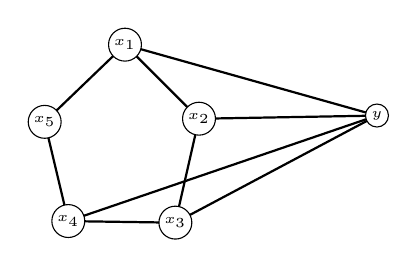
\begin{tikzpicture}[scale = 10]
\tikzstyle{VertexStyle}=[shape = circle,	
								 minimum size = 1pt,
								 inner sep = 1.2pt,
                         draw]
\Vertex[x = 0.491999983787537, y = 0.856000006198883, L = \tiny {$x_1$}]{v0}
\Vertex[x = 0.586000025272369, y = 0.761999994516373, L = \tiny {$x_2$}]{v1}
\Vertex[x = 0.389999985694885, y = 0.758000001311302, L = \tiny {$x_5$}]{v2}
\Vertex[x = 0.420000016689301, y = 0.631999999284744, L = \tiny {$x_4$}]{v3}
\Vertex[x = 0.555999994277954, y = 0.629999965429306, L = \tiny {$x_3$}]{v4}
\Vertex[x = 0.811999976634979, y = 0.765999987721443, L = \tiny {$y$}]{v5}
\Edge[](v1)(v0)
\Edge[](v1)(v4)
\Edge[](v4)(v3)
\Edge[](v2)(v3)
\Edge[](v0)(v2)
\Edge[](v5)(v0)
\Edge[](v5)(v1)
\Edge[](v5)(v4)
\Edge[](v5)(v3)
\end{tikzpicture}
\caption{The graph $N_6$.}
\label{fig:N6}
\end{figure}


\begin{lem}\label{N6Choosable}
The graph $\join{K_1}{N_6}$ where $N_6$ is the graph in Figure \ref{fig:N6} is
$d_1$-choosable.
\end{lem}
\begin{proof}
Suppose not and let $L$ be a minimal bad $d_1$-assignment on $\join{K_1}{N_6}$. 
Then, by the Small Pot Lemma, $\card{Pot(L)} \leq 6$.  Let $v$ be the vertex in
the $K_1$.  Note that $|L(v)|=5$, $|L(y)|=4$, $|L(x_5)|=2$, and $|L(x_i)|=3$ for
all $i\in[4]$.  Since $\sum_{i=1}^5|L(x_i)| = 14 > |Pot(L)|\omega(C_5)$, we see
that two nonadjacent $x_i$'s have a common color.  Hence, by Lemma
\ref{NeighborhoodPotShrink}, we have $\card{Pot(L)} \leq 5$. Thus we have $c
\in L(y) \cap L(x_5)$.  Also, $L(x_1) \cap L(x_4) \neq \emptyset$, $L(x_1) \cap
L(x_3) \neq \emptyset$ and $L(x_2) \cap L(x_4) \neq \emptyset$.  By Lemma
\ref{IntersectionsInB}, the common color in all of these sets must be $c$. 
Hence $c$ is in all the lists.

Now consider the list assignment $L'$ where $L'(z) = L(z) - c$ for all $z \in
N_6$.  Then $\card{Pot(L')} = 4$ and since $\sum_{i=1}^5|L'(x_i)| = 9 >
|Pot(L')|\omega(C_5)$, we see that that nonadjacent $x_i$'s have a common
color different than $c$.  Now appling Lemma \ref{IntersectionsInB} gives a
final contradiction.
\end{proof}

By a \emph{thickening} of a graph $G$, we just mean a graph formed by replacing
each $x \in V(G)$ by a complete graph $T_x$ such that $\card{T_x} \geq 1$ and
for $x,y \in V(G)$, $T_x$ is joined to $T_y$ iff $x \adj y$.

\begin{lem}\label{BisimplicialOrThickC5}
Any graph $H$ with $\alpha(H) \leq 2$ such that every
induced subgraph of $\join{K_1}{H}$ is not $d_1$-choosable can either be covered
by two cliques or is a thickening of $C_5$.
\end{lem}
\begin{proof}
Suppose not and let $H$ be a counterexample.

\textbf{Claim~1.} \textit{$\join{K_1}{H}$ is $d_0$-choosable.}
Otherwise $\join{K_1}{H}$ is a Gallai tree with a universal vertex.  Since
$\alpha(H)\le 2$,
$\join{K_1}{H}$ has at most two blocks and they must be complete. Hence $H$ can
be covered by two cliques, a contradiction.  Claim~1 will allow us to apply
Lemma~\ref{IntersectionsInB} below.

\textbf{Claim~2.} \textit{$H$ contains an induced $C_4$ or an induced $C_5$.}
Suppose not.  Then $H$ must be chordal since $\alpha(H) \leq 2$.  In particular,
$H$ contains a simplicial vertex $x$.  But then $\set{x} \cup N_H(x)$ and $V(H)
- N_H(x) - \set{x}$ are two cliques covering $H$, a contradiction.

\textbf{Claim~3.} \textit{$H$ does not contain an induced $C_5$ together with a vertex joined to at least
$4$ vertices in the $C_5$.}
Suppose the contrary.  If the vertex is joined to all of the $C_5$, then we have
a induced $\join{K_2}{C_5}$, which is $d_1$-choosable by
Lemma~\ref{K2Classification}. If the vertex is joined to only four vertices in
the $C_5$, we have an induced $\join{K_1}{N_6}$, impossible by Lemma
\ref{N6Choosable}.

\textbf{Claim~4.} \textit{$H$ contains no induced $C_4$.}
Suppose otherwise that $H$ contains an induced $C_4$, say $x_1x_2x_3x_4x_1$. 
Put $R \DefinedAs V(H) - \set{x_1, x_2, x_3, x_4}$.  Let $y \in R$. As
$\alpha(H) \leq 2$, $y$ has a neighbor in $\set{x_1, x_3}$ and a neighbor in
$\set{x_2, x_4}$.  If $y$ is adjacent to all of $x_1, \ldots, x_4$, then
$\join{K_1}{H}$ contains $\join{K_2}{C_4}$ which is $d_1$-choosable, impossible.
If $y$ is adjacent to three of $x_1, \ldots, x_4$, then $\join{K_1}{H}$ contains
$\join{E_2}{\text{paw}}$ which is $d_1$-choosable, impossible.

Thus every $y \in R$ is adjacent to all and only the vertices on one side of the
$C_4$.  We show that any two vertices in $R$ must be adjacent to the same or
opposite side and this gives the desired covering by two cliques.  If this
doesn't happen, then by symmetry we may suppose we have $y_1, y_2 \in R$ such
that $y_1 \adj x_1, x_2$ and $y_2 \adj x_2, x_3$.  We must have $y_1 \adj y_2$
for otherwise $\set{y_1, y_2, x_4}$ is an independent set.  But now $x_1y_1
y_2x_3x_4x_1$ is an induced $C_5$ in which $x_2$ has $4$ neighbors, impossible
by Claim~3.

\textbf{Claim~5.} \textit{$H$ does not exist.}
By Claim~2 and Claim~4, $H$ contains an induced
$C_5$. That $H$ is a thickening of this $C_5$ is now is immediate from
$\alpha(H) \leq 2$ and Claim~3.  This final contradiction
completes the proof.
\end{proof}

\begin{figure}[htb]
\centering
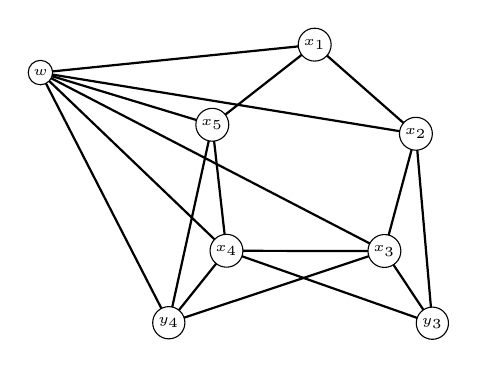
\begin{tikzpicture}[scale = 10]
\tikzstyle{VertexStyle}=[shape = circle,	
								 minimum size = 1pt,
								 inner sep = 1.2pt,
                         draw]
\Vertex[x = 0.535568237304688, y = 0.836275801062584, L = \tiny {$x_2$}]{v0}
\Vertex[x = 0.294997036457062, y = 0.687704384326935, L = \tiny {$x_4$}]{v1}
\Vertex[x = 0.495568662881851, y = 0.687386810779572, L = \tiny {$x_3$}]{v2}
\Vertex[x = 0.276996433734894, y = 0.847704276442528, L = \tiny {$x_5$}]{v3}
\Vertex[x = 0.556489169597626, y = 0.595672339200974, L = \tiny {$y_3$}]{v4}
\Vertex[x = 0.0587111786007881, y = 0.913989931344986, L = \tiny {$w$}]{v5}
\Vertex[x = 0.221746027469635, y = 0.596272975206375, L = \tiny {$y_4$}]{v6}
\Vertex[x = 0.407015770673752, y = 0.949415870010853, L = \tiny {$x_1$}]{v7}
\Edge[](v2)(v0)
\Edge[](v2)(v1)
\Edge[](v3)(v1)
\Edge[](v4)(v1)
\Edge[](v0)(v5)
\Edge[](v1)(v5)
\Edge[](v2)(v5)
\Edge[](v3)(v5)
\Edge[](v4)(v2)
\Edge[](v4)(v0)
\Edge[](v6)(v1)
\Edge[](v6)(v5)
\Edge[](v6)(v3)
\Edge[](v6)(v2)
\Edge[](v7)(v3)
\Edge[](v7)(v0)
\Edge[](v7)(v5)
\end{tikzpicture}
\caption{The graph $D_8$.}
\label{fig:D8}
\end{figure}


\begin{lem}\label{D8Choosable}
The graph $D_8$ is $d_1$-choosable.
\end{lem}
\begin{proof}
Suppose not and let $L$ be a minimal bad
$d_1$-assignment on $G \DefinedAs D_8$. 

\textbf{Claim~1.} \textit{$|Pot(L)|\le 6$.} By the Small Pot Lemma, we know that
$\card{Pot(L)}\le 7$.  Suppose $\card{Pot(L)} = 7$.  Say $Pot(L) - L(w) =
\set{a,b}$.  

We must have $L(y_3) = \set{a,b}$. Otherwise we could color $y_3$ from 
$L(y_3) - \set{a,b}$ and note that $G-y_3-w$
is $d_0$-choosable and hence has a coloring from its lists.  Then we can easily
modify this coloring to use both $a$ and $b$ at least once.  But now we can
color $w$.

If there exist distinct vertices $u,v\in V(G)-y_3$ such that $a \in L(u)$, $b
\in L(v)$ and $\{u,v\}\not\subseteq \{x_2,x_3,x_4\}$, then we can color $G$ as
follows.  Color $y_3$ arbitrarily to leave $a$ available on $u$ and
$b$ available on $v$.  Again, $G-y_3-w$ has a coloring.  We can modify it to
use $a$ and $b$, then color $w$.  Thus, $a$ and $b$ each appear only on
some subset of $\{y_3,x_2,x_3,x_4\}$.  

If $a\in L(x_2)\cap L(x_4)$, then we use $a$ on $x_2$ and $x_4$ and color
greedily $y_3$, $x_3$, $y_4$, $x_1$, $x_5$, $w$ (actually any order will work
if $y_3$ is first and $w$ is last).   If $a$ appears only on $y_3$ and exactly
one neighbor $x_i$, then we violate Lemma \ref{ComponentsOfColor}
since $\card{Pot_{y_3, x_i}(L)} < 7$. So now $a$ appears precisely on either
$y_3,x_2,x_3$ or $y_3,x_3,x_4$. Similarly $b$ appears precisely on either
$y_3,x_2,x_3$ or $y_3,x_3,x_4$.

If $\{a,b\}\cap L(x_2)=\emptyset$, then we use $a$ on $y_3$ and $b$ on $x_3$,
then greedily color $y_4$, $x_4$, $x_5$, $x_1$, $w$, $x_2$.  By symmetry, we may
assume that $a \in L(x_2)$. But then since $\set{a,b} \subseteq L(x_3)$ we
have $\card{Pot_{y_3, x_2, x_3}(L)} < 7$ violating Lemma
\ref{ComponentsOfColor}.  Hence $\card{Pot(L)} \leq 6$.

\textbf{Claim~2.} \textit{$|Pot(L)|\le 5$.}  Suppose $\card{Pot(L)}=6$.  Choose $a
\in Pot(L) - L(w)$ and $b \in L(w) \cap L(y_3)$.  Put $H \DefinedAs G - y_3 -
w$.

First we show that $b\in L(x_2)\cap L(x_3)\cap L(x_4)$.  If not, we use $b$ on
$y_3$ and $w$, then greedily color $x_1$, $x_5$, $y_4$.  Now we can finish by
coloring last the $x_i$ such that $b\notin L(x_i)$.

We must have $a \in L(y_3)$ or else we color $x_2, x_4$ with $b$ and something
else in $H$ with $a$ (since $G_a$ contains an edge by Lemma \ref{ComponentsOfColor}) and
finish.  Now $a \not \in L(x_1), L(x_5), L(y_4)$, for
otherwise we color $x_2, x_4$ with $b$, $y_3$ with $a$ and then color $x_1, x_5,
y_4, x_3$ in order using $a$ when we can, then color $w$.  Now $a$ is
on $y_3$ and at least two of $x_2, x_3, x_4$ or else we violate Lemma
\ref{ComponentsOfColor}.  Now $a \not \in L(x_2) \cap L(x_4)$ since otherwise we
color $x_2, x_4$ with $a$, then $y_3$ with $b$, then greedily color $x_1, x_5,
y_4, x_3, w$.  Also $a \not \in L(x_2) \cap L(x_3)$ since then $\set{a,b}
\subseteq L(y_3) \cap L(x_2) \cap L(x_3)$ and hence $\card{Pot_{y_3, x_2,
x_3}(L)} < 6$ violating Lemma \ref{ComponentsOfColor}.  Therefore $V(G_a) =
\set{y_3, x_3, x_4}$.

Now $\card{Pot_{y_3, x_3, x_4}}(L) \leq 6$ and hence
$L(x_3) \cap L(x_4) = \set{a,b}$ for otherwise we violate Lemma
\ref{ComponentsOfColor}.  Say $L(x_3) = \set{a,b,c,d}$ and $L(x_4) =
\set{a,b,e,f}$. Then by symmetry $L(x_1)$ contains either $c$ or $e$.  
If $c \in L(x_1)$, color $x_1, x_3$ with $c$, $x_4$ with $a$ and $y_3$ with $b$.
Now we can greedily finish.  If $e \in L(x_1)$, color $x_1, x_4$ with $e$,
$x_3$ with $a$ and $y_3$ with $b$, again we can greedily finish.  Hence
$\card{Pot(L)} \leq 5$.

\textbf{Claim~3.} \textit{$L$ does not exist.}  Since $\card{Pot(L)} \leq 5$ we
see that $x_3, x_5$ have two colors in common and $x_2, x_4$ have two colors in
common as well. In fact, these sets of common colors must be the same and equal
$L(y_3) \DefinedAs \set{a,b}$ or we can finish the coloring. Similarly, we may
assume that $a \in L(y_4)$ (if $\{a,b\}\cap L(y_4)=\emptyset$, then we have
$L(x_2)\cap L(y_3)\cap (Pot(L)\setminus\{a,b\})\ne \emptyset$ and color $a$ on
$x_3, x_5$, so we can color $y_3$ with $b$ and then finish by
Lemma~\ref{IntersectionsInB}).
Similarly, $L(x_1)$ contains $a$ or $b$.  But it can't
contain $a$ for then we could color $y_3, y_4, x_1$ with $a$, and $x_2, x_4$ with
$b$, and then finish greedily. Say $L(x_4) = \set{a,b,c,d}$. Then as no nonadjacent
pair has a color in common that is in $Pot(L) - \set{a,b}$ we have $L(x_2) =
\set{a,b,e}$, then by symmetry of $c$ and $d$ we have $L(x_5) = \set{a,b,c}$.
Then $L(x_3) = \set{a,b,d,e}$ and hence $L(x_1) = \set{a,b}$, which contradicts
that $a\notin L(x_1)$.
%Now color $x_1, y_3, y_4$ with $a$ and $x_3, x_5$ with $b$.  
%Now greedily color with $w$ last to finish the coloring. 
We conclude that $L$ cannot exist.
\end{proof}

\begin{lem}\label{TwoTwoOneTwoOne}
Let $H$ be a thickening of $C_5$ such that $\card{H} \geq 6$. Then
$\join{K_1}{H}$ is $f$-choosable where $f(v) \geq d(v)$ for the $v$ in the $K_1$
and $f(x) \geq d(x) - 1$ for $x \in V(H)$.
\end{lem}
\begin{proof}
Suppose not and let $L$ be a minimal bad $f$-assignment on $\join{K_1}{H}$. By
the Small Pot Lemma, $\card{Pot(L)} \leq \card{H}$. Note that $H$ is
$d_0$-choosable since it contains an induced diamond. 
Let $x_1, \ldots, x_5$ be the vertices of an induced $C_5$ in $H$.  Then $\sum_i
\card{L(x_i)} = \sum_i d_H(x_i) = 3\card{H} - 5 > 2\card{H} \geq \omega(H[x_1,
\ldots, x_5])\card{Pot(L)}$ and hence some nonadjacent pair in $\set{x_1, \ldots, x_5}$ have a color in
common.  Now applying Lemma \ref{LowSinglePair} gives a contradiction.
\end{proof}

We are now in a position to finish the proof of Borodin-Kostochka for claw-free
graphs.

\begin{thm}\label{BKClawFree}
Every claw-free graph satisfying $\chi \geq \Delta \geq 9$ contains a
$K_\Delta$.
\end{thm}
\begin{proof}
Suppose not and choose a counterexample $G$ minimizing $\card{G}$.  Then $G$ is
vertex critical and not quasi-line by Lemma \ref{QuasiLineColoring}.  Hence $G$
contains a vertex $v$ that is not bisimplicial.  By Lemma
\ref{BisimplicialOrThickC5}, $G_v \DefinedAs G[N(v)]$ is a thickening of a
$C_5$.  Also, by Lemma \ref{TwoTwoOneTwoOne}, $v$ is high. Pick a $C_5$ in
$G_v$ and label its vertices $x_1, \ldots, x_5$ in clockwise order.  For $i \in \irange{5}$, let $T_i$ be the thickening clique
containing $x_i$.  Also, let $S$ be those vertices in $V(G) - N(v) - \set{v}$
that have a neighbor in $\set{x_1, \ldots, x_5}$.  First we establish a few
properties of vertices in $S$. 

\textbf{Claim~1.} \textit{For each $z \in S$ there is $i \in \irange{5}$ such that $N(z) \cap \set{x_1, \ldots, x_5} \in \{\set{x_i, x_{i+1}}, \set{x_i, x_{i+1}, x_{i+2}}\}$.} 
Let $z \in S$ and put $N \DefinedAs N(z) \cap \set{x_1, \ldots, x_5}$.  If
$\card{N} \geq 4$, then some subset of $\set{v, z} \cup N$ induces the
$d_1$-choosable graph $\join{E_2}{P_4}$.  Hence $\card{N} \leq 3$.  Since $G$ is
claw-free, the vertices in $N$ must be contiguous.

\textbf{Claim~2.} \textit{If $z \in S$ is adjacent to $x_i, x_{i+1}, x_{i+2}$, then $\card{T_i} =
\card{T_{i+1}} = \card{T_{i+2}} = 1$.}
Suppose not. First, lets deal with the case when $\card{T_{i+1}} \geq 2$.  Pick
$y \in T_{i+1} - x_{i+1}$.  If $y \nonadj z$, then $\set{x_i, y, z, x_{i-1}}$
induces a claw, impossible.  Thus $y \adj z$ and $\set{v, z, x_i, x_{i+1},
x_{i+2}, y}$ induces the $d_1$-choosable graph $\join{E_2}{\text{diamond}}$.

Hence, by symmetry, we may assume that $\card{T_i} \geq 2$.  Now, if $y \nonadj z$,
then $\{v, x_1, \ldots, x_5, y, z\}$ induces a $D_8$ contradicting Lemma
\ref{D8Choosable}.  Hence $y \adj z$ and $\set{v, z, x_i, x_{i+1},
x_{i+2}, y}$ induces the $d_1$-choosable graph $\join{E_2}{\text{paw}}$, a
contradiction.

\textbf{Claim~3.} \textit{For $i \in \irange{5}$, let $B_i$ be the $z \in S$ with
$N(z) \cap \set{x_1, \ldots, x_5} = \set{x_i, x_{i+1}}$.  Then $B_i \cup B_{i+1}$ and $B_i \cup T_i \cup T_{i+1}$ both induce cliques for any
$i \in \irange{5}$.}
Otherwise there would be a claw.

\textbf{Claim~4.} \textit{$\card{T_i} \leq 2$ for all $i \in \irange{5}$.}
Suppose otherwise that we have $i$ such that $\card{T_i} \geq 3$.  Put $A_i
\DefinedAs N(x_i) \cap S$. By Claim~2, $A_i \subseteq
B_{i-1} \cup B_i$ and $A_i$ is joined to $T_i$.  Thus $T_i$ is joined to $F_i
\DefinedAs \set{v} \cup A_i \cup T_{i-1} \cup T_{i+1}$.  If $A_i\ne\emptyset$,
then $F_i$ induces a graph that is connected and not almost complete, so this
is impossible by Lemma \ref{K3Classification}.   If $A_i = \emptyset$, then
$x_i$ must have at least $\Delta - 2$ neighbors in $T_{i-1} \cup T_i \cup
T_{i+1}$.  But that leaves at most one vertex for $T_{i-2} \cup T_{i+2}$,
impossible.

\textbf{Claim~5.} \textit{$G$ does not exist.}
Since $d(v) = \Delta \geq 9$, by symmetry we may assume that $\card{T_i} = 2$
for all $i \in \irange{4}$.  As in the proof of Claim~4, we get that $T_2$ is joined to $F_2$. Since $|T_i|\le 2$ for all $i$, we must have $A_i\ne \emptyset$ (for all $i$,
but in particular for $A_2$). Since $A_i\subseteq B_{i-1}\cup B_i$, by symmetry,
we may assume that $A_2 \cap B_2 \neq \emptyset$. Pick $z \in A_2 \cap B_2$ and $y_i \in T_i - x_i$ for $i \in \irange{3}$. 
Then $F_2$ has the graph in Figure \ref{fig:FinalContradiction} as an induced subgraph, but this is impossible by Lemma \ref{K2Classification}.
\end{proof}
  
\begin{figure}[htb]
\centering
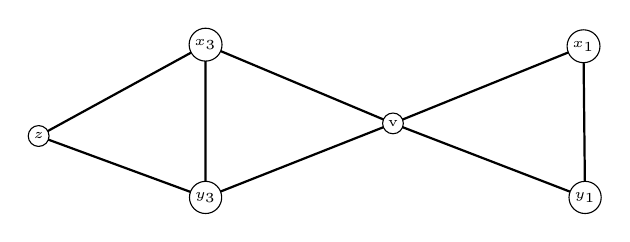
\begin{tikzpicture}[scale = 10]
\tikzstyle{VertexStyle}=[shape = circle,	
								 minimum size = 1pt,
								 inner sep = 1.2pt,
                         draw]
\Vertex[x = 0.89000016450882, y = 0.730000019073486, L = \tiny {$x_1$}]{v0}
\Vertex[x = 0.410000026226044, y = 0.538000077009201, L = \tiny {$y_3$}]{v1}
\Vertex[x = 0.648000001907349, y = 0.631999969482422, L = \tiny {v}]{v2}
\Vertex[x = 0.409999966621399, y = 0.731999933719635, L = \tiny {$x_3$}]{v3}
\Vertex[x = 0.892000138759613, y = 0.537999987602234, L = \tiny {$y_1$}]{v4}
\Vertex[x = 0.198000028729439, y = 0.616000115871429, L = \tiny {$z$}]{v5}
\Edge[](v0)(v2)
\Edge[](v1)(v2)
\Edge[](v3)(v1)
\Edge[](v3)(v2)
\Edge[](v4)(v0)
\Edge[](v4)(v2)
\Edge[](v5)(v3)
\Edge[](v5)(v1)
\end{tikzpicture}
\caption{$K_2$ joined to this graph is $d_1$-choosable}
\label{fig:FinalContradiction}
\end{figure}


We note that this reduction to the quasi-line case also works for the
Borodin-Kostochka conjecture for list coloring; that is, we have the following
result.

\begin{thm}\label{ClawFreeLiftForLists}
If every quasi-line graph satisfying $\chi_l \geq \Delta \geq 9$ contains a
$K_\Delta$, then the same statement holds for every claw-free graph.
\end{thm}



\chapter{MULES}\label{APrioriWowChapter}
\begin{center}
\emph{The material in this chapter appeared in \cite{mules} and is joint work with Dan Cranston.}
\end{center}

In this we chapter carry out an in-depth study of minimum counterexamples to the
Borodin-Kostochka conjecture.  Our main tool is the classification, in Chapter
\ref{ListColoringChapter}, of graph joins $\join{A}{B}$ with $|A|\ge 2$, $|B|\ge
2$ which are $f$-choosable, where $f(v) \DefinedAs d(v) - 1$ for each vertex
$v$.  Since such a join cannot be an induced subgraph of a vertex critical
graph with $\chi = \Delta$, we have a wealth of structural information about
minimum counterexamples to the Borodin-Kostochka conjecture.  In Section
\ref{excludemule}, we exploit this information and minimality to improve Reed's
Lemma \ref{ReedsLemma} as follows (see Corollary~\ref{AtMostOneEdgeIn}).

\begin{lem}
Let $G$ be a vertex critical graph satisfying $\chi = \Delta \geq 9$ having the
minimum number of vertices. 
If $H$ is a $K_{\Delta - 1}$ in $G$, then any vertex in $G - H$ has at most $1$
neighbor in $H$.
\end{lem}

Moreover, we lift the result out of the context of a minimum counterexample to
the Borodin-Kostochka conjecture, to the more general context of graphs
satisfying a certain criticality condition---we call such graphs mules. This allows us to prove meaningful results for values of $\Delta$ less than
$9$.  

Since a graph containing $K_\Delta$ as a subgraph also
contains $K_{t, \Delta - t}$ as a subgraph for any $t \in \irange{\Delta - 1}$,
the Borodin-Kostochka conjecture implies the following conjecture.  Our main
result in this chapter is that the two conjectures are equivalent.

\begin{conjecture}\label{NoThreeDealEquiv}
Any graph with $\chi = \Delta \geq 9$ contains some $\join{A_1}{A_2}$ as an
induced subgraph where $\card{A_1}, \card{A_2} \geq 3$, $\card{A_1} + \card{A_2} = \Delta$
and $A_i \neq \djunion{K_1}{K_{\card{A_i} - 1}}$ for some $i \in \irange{2}$.
\end{conjecture}

In fact, using Kostochka's reduction (Lemma~\ref{HereditaryReduction}) to the
case $\Delta = 9$, the following conjecture is also equivalent.

\begin{conjecture}
Any graph with $\chi = \Delta = 9$ contains some $\join{A_1}{A_2}$ as an induced
subgraph where $\card{A_1}, \card{A_2} \geq 3$, $\card{A_1} + \card{A_2} = 9$
and $A_i \neq \djunion{K_1}{K_{\card{A_i} - 1}}$ for some $i \in \irange{2}$.
\end{conjecture}

As a special case, we get a couple more palatable equivalent conjectures (see
Lemma~\ref{K3sOut} and the comment following it).

\begin{conjecture}\label{K3Conjecture}
Any graph with $\chi = \Delta \geq 9$ contains $\join{K_3}{E_{\Delta-3}}$ as a
subgraph.
\end{conjecture}

\begin{conjecture}\label{K3ConjectureReduced}
Any graph with $\chi = \Delta = 9$ contains $\join{K_3}{E_6}$ as a
subgraph.
\end{conjecture}

The condition $A_i \neq \djunion{K_1}{K_{\card{A_i} - 1}}$ is unnatural and
by removing it we get a (possibly) weaker conjecture than the
Borodin-Kostochka conjecture which has more aesthetic appeal.

\begin{conjecture}\label{NonInducedThreeDeal}
Let $G$ be a graph with $\Delta(G) = k \geq 9$. If $K_{t, k - t} \not \subseteq G$ for all $3 \leq t \leq k - 3$, then $G$ can be $(k - 1)$-colored.
\end{conjecture}

\begin{conjecture}
Conjecture \ref{NonInducedThreeDeal} is equivalent to the Borodin-Kostochka
conjecture.
\end{conjecture}

Perhaps it would be easier to attack Conjecture \ref{NonInducedThreeDeal} with
$3 \leq t \leq k - 3$ replaced by $2 \leq t \leq k - 2$?  We are unable to
prove even this conjecture. Making this change and bringing $k$ down to $5$
gives the following conjecture, which, if true, would imply the remaining two cases of Gr\"unbaum's girth problem for graphs with girth at least five.

\begin{conjecture}\label{NonInducedTwoDeal}
Let $G$ be a graph with $\Delta(G) = k \geq 5$. If $K_{t, k - t} \not \subseteq
G$ for all $2 \leq t \leq k - 2$, then $G$ can be $(k - 1)$-colored.
\end{conjecture}

If $G$ is a graph with with $\Delta(G) = k \geq 5$ and girth at least five, then
it contains no $K_{t, k - t}$ for all $2 \leq t \leq k - 2$ and hence Conjecture \ref{NonInducedTwoDeal} would give a
$(k-1)$-coloring.  This conjecture would be tight since the Gr\"unbaum graph and
the Brinkmann graph are examples with $\chi = \Delta = 4$ and girth at least
five.

Finally, we prove that the following conjecture is equivalent to the
Borodin-Kostochka conjecture for graphs with independence number at most $6$
(see Theorem~\ref{SmallAlphaConj}).

\begin{conjecture}\label{AlphaConjecture}
Every graph satisfying $\chi = \Delta = 9$ and $\alpha \leq 6$ contains a
$K_{8}$.
\end{conjecture}

\section{What is a mule?}
\begin{defn}
If $G$ and $H$ are graphs, an \emph{epimorphism} is a graph homomorphism $\funcsurj{f}{G}{H}$ such that $f(V(G)) = V(H)$.  We indicate this with the arrow $\surj$.
\end{defn}

\begin{defn}
Let $G$ be a graph.  A graph $A$ is called a \emph{child} of $G$ if $A \neq G$ and there exists $H \unlhd G$ and an epimorphism $\funcsurj{f}{H}{A}$.  
\end{defn}

Note that the child-of relation is a strict partial order on the set of (finite simple) graphs $\fancy{G}$.  
We call this the \emph{child order} on $\fancy{G}$ and denote it by `$\prec$'.  By definition, if $H \lhd G$ then $H \prec G$.

\begin{lem}\label{well-founded}
The ordering $\prec$ is well-founded on $\fancy{G}$; that is, every nonempty subset of $\fancy{G}$ has a minimal element under $\prec$.
\end{lem}
\begin{proof}
Let $\fancy{T}$ be a nonempty subset of $\fancy{G}$.  Pick $G \in \fancy{T}$ minimizing $\card{G}$ and then maximizing $\size{G}$.  
Since any child of $G$ must have fewer vertices or more edges (or both), we see that $G$ is minimal in $\fancy{T}$ with respect to $\prec$.
\end{proof}

\begin{defn}
Let $\fancy{T}$ be a collection of graphs.  A minimal graph in $\fancy{T}$ under the child order is called a \emph{$\fancy{T}$-mule}.
\end{defn}

With the definition of mule we have captured the important properties (for coloring) of a counterexample first 
minimizing the number of vertices and then maximizing the number of edges.  Viewing $\fancy{T}$ as a set of counterexamples, 
we can add edges to or contract independent sets in induced subgraphs of a $\fancy{T}$-mule and get a non-counterexample.  
We could do the same with a minimal counterexample, but with mules we have more minimal objects to work with. 
One striking consequence of this is that many of our proofs naturally construct multiple counterexamples to Borodin-Kostochka for small $\Delta$.

\section{Excluding induced subgraphs in mules}\label{excludemule}
Our main goal in this section is to prove Lemma~\ref{K4sOut}, which says that (with
only one exception) for $k\ge 7$, no $k$-mule contains $\join{K_4}{E_{k-4}}$ as
a subgraph.  This result immediately implies that the Borodin-Kostochka
conjecture is equivalent to Conjecture~\ref{K4Conjecture}.  This equivalence is
a major step toward our main result.  Our approach is
based on Lemma~\ref{K_tClassification}, which implies that if $G$ is a
counterexample to Lemma~\ref{K4sOut}, then the vertices of the $E_{k-4}$ induce either
$E_3$, a claw, a clique, or an almost complete graph.  Our job in this section
consists of showing that each of these four possibilities is, in fact,
impossible.  Ruling out the clique is easy.  The cases of $E_3$ and the claw
are handled in Lemma~\ref{NoE3}, and the case of an almost complete graph
(which requires the most work) is handled by Corollary~\ref{AtMostOneEdgeIn}.
\bigskip

For $k \in \IN$, by a \emph{$k$-mule} we mean a $\C{k}$-mule.

\begin{lem}\label{EpiPower}
Let $G$ be a $k$-mule with $k \geq 4$.  If $A$ is a child of $G$ with $\Delta(A) \leq k$ then either
\begin{itemize}
\item $A$ is $(k - 1)$-colorable; or,
\item $A$ contains a $K_k$.
\end{itemize}
\end{lem}
\begin{proof}
Let $A$ be a child of $G$ with $\Delta(A) \leq k$, $H \unlhd G$ and $\funcsurj{f}{H}{A}$ an epimorphism.  
Without loss of generality, $A$ is vertex critical. Suppose $A$ is not $(k - 1)$-colorable.  
Then $\chi(A) \geq k \geq \Delta(A)$.  Since $A \prec G$ and $G$ is a mule, $A \not \in \C{k}$. 
Thus we have $\chi(A) > \Delta(A) \geq 3$, so Brooks' theorem implies that 
$A = K_k$.
\end{proof}

Note that adding edges to a graph yields an epimorphism.

\begin{lem}\label{UnequalColoredPairOrCliqueMinusEdge}
Let $G$ be a $k$-mule with $k \geq 4$ and $H \unlhd G$.  
Assume $x, y \in V(H)$, $xy \not \in E(H)$ and both $d_H(x) \leq k-1$ and $d_H(y) \leq k-1$. 
If for every $(k - 1)$-coloring $\pi$ of $H$ we have $\pi(x) = \pi(y)$, then $H$ contains $\join{\set{x, y}}{K_{k-2}}$.
\end{lem}
\begin{proof}
Suppose that for every $(k - 1)$-coloring $\pi$ of $H$ we have $\pi(x) = \pi(y)$.
Using the inclusion epimorphism $\funcsurj{f_{xy}}{H}{H + xy}$ in Lemma \ref{EpiPower} shows that either $H + xy$ is $(k - 1)$-colorable or $H + xy$ contains a $K_k$.  
Since a $(k - 1)$-coloring of $H + xy$ would induce a $(k - 1)$-coloring of $H$ with $x$ and $y$ colored differently, we conclude that $H + xy$ contains a $K_k$.  
But then $H$ contains $\join{\set{x, y}}{K_{k-2}}$ and the proof is complete.
\end{proof}

We will often begin by coloring some subgraph $H$ of our graph $G$, and work to
extend this partial coloring.  More formally, let $G$ be a graph and $H \lhd G$.  For $t \geq \chi(H)$, let $\pi$ be a proper $t$-coloring of $H$.  
For each $x \in V(G-H)$, put $L_{\pi}(x) \DefinedAs \set{1, \ldots, t} -
\bigcup_{y \in N(x) \cap V(H)} \pi(y)$. Then $\pi$ is completable to a
$t$-coloring of $G$ iff $L_{\pi}$ admits a coloring of $G-H$. 
We will use this fact repeatedly in the proofs that follow.  The following
generalizes a lemma due to Reed \cite{reed1999strengthening}, the proof is
essentially the same.

\begin{lem}\label{E2impliesE3}
For $k \geq 6$, if a $k$-mule $G$ contains an induced $\join{E_2}{K_{k - 2}}$, then $G$ contains an induced $\join{E_3}{K_{k - 2}}$.
\end{lem}
\begin{proof}
Suppose $G$ is a $k$-mule containing an induced $\join{E_2}{K_{k - 2}}$, call it $F$.  
Let $x, y$ be the vertices of degree $k-2$ in $F$ and $C \DefinedAs \set{w_1,
\ldots, w_{k-2}}$ the vertices of degree $k-1$ in $F$.  Put $H \DefinedAs G -
F$. Since $G$ is vertex critical, we may $k-1$ color $H$.  Doing so leaves a list assignment $L$ on $F$ with $\card{L(z)} \geq d_F(z) - 1$ for each $z \in V(F)$. 
Now $\card{L(x)} + \card{L(y)} \geq d_F(x) + d_F(y) - 2 = 2k - 6 > k - 1$ since $k \geq 6$.  Hence we have $c \in L(x) \cap L(y)$.  
Coloring both $x$ and $y$ with $c$ leaves a list assignment $L'$ on $C$ with $\card{L'(w_i)} \geq k - 3$ for each $1 \leq i \leq k-2$.  
Now, if $\card{L'(w_i)} \geq k - 2$ or $L'(w_i) \neq L'(w_j)$ for some $i, j$, then we can complete the partial $(k - 1)$-coloring to all of $G$ using Hall's Theorem.  
Hence we must have $d(w_i) = k$ and $L'(w_i) = L'(w_j)$ for all $i,j$.  
Let $N \DefinedAs \bigcup_{w \in C} N(w) \cap V(H)$ and note that $N$ is an
independent set since it is contained in a single color class in every $(k - 1)$-coloring of $H$. Also, each $w \in C$ has exactly one neighbor in $N$.

Proving that $\card{N} = 1$ will give the desired $\join{E_3}{K_{k - 2}}$ in $G$.  Thus, to reach a contradiction, suppose that $\card{N} \geq 2$.  

We know that $H$ has no $(k - 1)$-coloring in which two vertices of $N$ get different colors since then we could complete the partial coloring as above. 
Let $v_1, v_2 \in N$ be different. Since both $v_1$ and $v_2$ have a neighbor in $F$, we may apply Lemma \ref{UnequalColoredPairOrCliqueMinusEdge} to conlcude 
that $\join{\set{v_1, v_2}}{K_{v_1, v_2}}$ is in $H$, where $K_{v_1, v_2}$ is a $K_{k-2}$.

First, suppose $\card{N} \geq 3$, say $N = \set{v_1, v_2, v_3}$.  We have $z \in K_{v_1, v_2} \cap K_{v_1, v_3}$ for otherwise $d(v_1) \geq 2(k - 2) > k$.  
Since $z$ already has $k$ neighbors among $K_{v_1, v_2} - \set{z}$ and $v_1, v_2, v_3$, we must have $K_{v_1, v_3} = K_{v_1, v_2}$.  
But then $\set{v_1, v_2, v_3} + K_{v_1, v_2}$ is our desired $\join{E_3}{K_{k - 2}}$ in $G$.

Hence we must have $\card{N} = 2$, say $N = \set{v_1, v_2}$.  For $i \in \irange{2}$, $v_i$ has $k - 2$ neighbors in $K_{v_1, v_2}$ and thus at most two neighbors in $C$.  
Hence $\card{C} \leq 4$.  Thus we must have $k = 6$.

We may apply the same reasoning to $\join{\set{v_1, v_2}}{K_{v_1, v_2}}$ that we did to $F$ to get vertices $v_{2,1}, v_{2,2}$ 
such that $\join{\set{v_{2,1}, v_{2,2}}}{K_{v_{2,1}, v_{2,2}}}$ is in $G$.  But then we may do it again with $\join{\set{v_{2,1}, v_{2,2}}}{K_{v_{2,1}, v_{2,2}}}$ and so on.  
Since $G$ is finite, at some point this process must terminate. But the only way to terminate is to come back around and use $x$ and $y$.  
This graph is $5$-colorable since we may color all the $E_2$'s with the same color and then $4$-color the remaining $K_4$ components.  
This final contradiction completes the proof.
\end{proof}

\begin{figure}[htb]
\centering
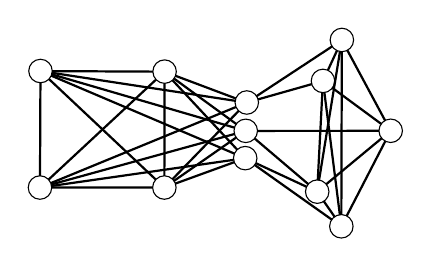
\begin{tikzpicture}[scale = 10]
\tikzstyle{VertexStyle}=[shape = circle,	
								 minimum size = 1pt,
								 inner sep = 3pt,
                         draw]
\Vertex[x = 0.25085711479187, y = 0.92838092893362, L = \tiny {}]{v0}
\Vertex[x = 0.0932380929589272, y = 0.929142817854881, L = \tiny {}]{v1}
\Vertex[x = 0.250571489334106, y = 0.781142801046371, L = \tiny {}]{v2}
\Vertex[x = 0.092571459710598, y = 0.781142845749855, L = \tiny {}]{v3}
\Vertex[x = 0.355238050222397, y = 0.889142841100693, L = \tiny {}]{v4}
\Vertex[x = 0.353904783725739, y = 0.853142827749252, L = \tiny {}]{v5}
\Vertex[x = 0.353238135576248, y = 0.818476170301437, L = \tiny {}]{v6}
\Vertex[x = 0.476000010967255, y = 0.968571435660124, L = \tiny {}]{v7}
\Vertex[x = 0.537999987602234, y = 0.853238105773926, L = \tiny {}]{v8}
\Vertex[x = 0.444666564464569, y = 0.77590474486351, L = \tiny {}]{v9}
\Vertex[x = 0.475333333015442, y = 0.731904745101929, L = \tiny {}]{v10}
\Vertex[x = 0.451999962329865, y = 0.916571423411369, L = \tiny {}]{v11}
\Edge[](v0)(v1)
\Edge[](v2)(v1)
\Edge[](v3)(v1)
\Edge[](v0)(v3)
\Edge[](v2)(v3)
\Edge[](v2)(v0)
\Edge[](v4)(v2)
\Edge[](v5)(v2)
\Edge[](v6)(v2)
\Edge[](v4)(v0)
\Edge[](v5)(v0)
\Edge[](v6)(v0)
\Edge[](v4)(v1)
\Edge[](v5)(v1)
\Edge[](v6)(v1)
\Edge[](v4)(v3)
\Edge[](v5)(v3)
\Edge[](v6)(v3)
\Edge[](v8)(v7)
\Edge[](v9)(v7)
\Edge[](v10)(v7)
\Edge[](v11)(v7)
\Edge[](v9)(v8)
\Edge[](v10)(v8)
\Edge[](v11)(v8)
\Edge[](v10)(v9)
\Edge[](v11)(v9)
\Edge[](v11)(v10)
\Edge[](v4)(v7)
\Edge[](v4)(v11)
\Edge[](v6)(v9)
\Edge[](v6)(v10)
\Edge[](v5)(v8)
\Edge[](v5)(v9)
\end{tikzpicture}
\caption{The mule $M_{6,1}$.}
\label{fig:M_61}
\end{figure}

\begin{figure}[htb]
\centering
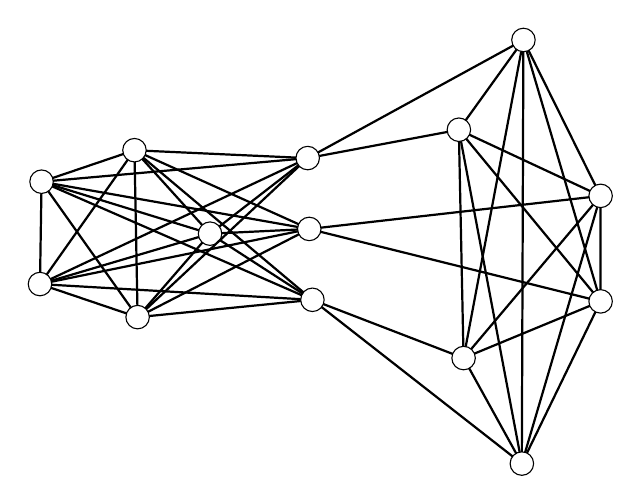
\begin{tikzpicture}[scale = 10]
\tikzstyle{VertexStyle}=[shape = circle,	
								 minimum size = 1pt,
								 inner sep = 3pt,
                         draw]
\Vertex[x = 0.751999914646149, y = 0.724000096321106, L = \tiny {}]{v0}
\Vertex[x = 0.751999974250793, y = 0.590000092983246, L = \tiny {}]{v1}
\Vertex[x = 0.652000069618225, y = 0.38400000333786, L = \tiny {}]{v2}
\Vertex[x = 0.578000009059906, y = 0.51800012588501, L = \tiny {}]{v3}
\Vertex[x = 0.572000086307526, y = 0.808000028133392, L = \tiny {}]{v4}
\Vertex[x = 0.0419999808073044, y = 0.742000013589859, L = \tiny {}]{v5}
\Vertex[x = 0.0399999916553497, y = 0.612000048160553, L = \tiny {}]{v6}
\Vertex[x = 0.163999989628792, y = 0.569999992847443, L = \tiny {}]{v7}
\Vertex[x = 0.25600004196167, y = 0.676000028848648, L = \tiny {}]{v8}
\Vertex[x = 0.159999996423721, y = 0.782000005245209, L = \tiny {}]{v9}
\Vertex[x = 0.653999924659729, y = 0.921999998390675, L = \tiny {}]{v10}
\Vertex[x = 0.379999995231628, y = 0.771999999880791, L = \tiny {}]{v11}
\Vertex[x = 0.381999999284744, y = 0.682000011205673, L = \tiny {}]{v12}
\Vertex[x = 0.386000007390976, y = 0.592000007629395, L = \tiny {}]{v13}
\Edge[](v0)(v4)
\Edge[](v1)(v4)
\Edge[](v2)(v4)
\Edge[](v3)(v4)
\Edge[](v0)(v3)
\Edge[](v1)(v3)
\Edge[](v2)(v3)
\Edge[](v0)(v2)
\Edge[](v1)(v2)
\Edge[](v0)(v1)
\Edge[](v5)(v6)
\Edge[](v5)(v7)
\Edge[](v5)(v8)
\Edge[](v5)(v9)
\Edge[](v6)(v7)
\Edge[](v6)(v8)
\Edge[](v6)(v9)
\Edge[](v7)(v8)
\Edge[](v7)(v9)
\Edge[](v8)(v9)
\Edge[](v0)(v10)
\Edge[](v1)(v10)
\Edge[](v2)(v10)
\Edge[](v3)(v10)
\Edge[](v4)(v10)
\Edge[](v5)(v11)
\Edge[](v6)(v11)
\Edge[](v7)(v11)
\Edge[](v8)(v11)
\Edge[](v9)(v11)
\Edge[](v5)(v12)
\Edge[](v6)(v12)
\Edge[](v7)(v12)
\Edge[](v8)(v12)
\Edge[](v9)(v12)
\Edge[](v5)(v13)
\Edge[](v6)(v13)
\Edge[](v7)(v13)
\Edge[](v8)(v13)
\Edge[](v9)(v13)
\Edge[](v11)(v10)
\Edge[](v11)(v4)
\Edge[](v12)(v0)
\Edge[](v12)(v1)
\Edge[](v13)(v3)
\Edge[](v13)(v2)
\end{tikzpicture}
\caption{The mule $M_{7,1}$.}
\label{fig:M_7}
\end{figure}


\begin{lem}\label{NoE2}
For $k \geq 6$, the only $k$-mules containing an induced $\join{E_2}{K_{k - 2}}$
are $M_{6,1}$ and $M_{7,1}$.
\end{lem}
\begin{proof}
Suppose we have a $k$-mule $G$ that contains an induced $\join{E_2}{K_{k - 2}}$. 
Then by Lemma \ref{E2impliesE3}, $G$ contains an induced $\join{E_3}{K_{k - 2}}$, call it $F$. 

Let $x, y, z$ be the vertices of degree $k-2$ in
$F$ and let $C \DefinedAs \set{w_1, \ldots, w_{k-2}}$ be the vertices of degree
$k$ in $F$. Put $H \DefinedAs G - C$. Since each of $x, y, z$ have degree at
most $2$ in $H$ and $G$ is a mule, the homomorphism from $H$ sending $x, y$, and
$z$ to the same vertex must produce a $K_k$.  Thus we must have $k \leq 7$ and
$H$ contains a $K_{k-1}$ (call it $D$) such that $V(D) \subseteq N(x) \cup N(y)
\cup N(z))$.  Put $A \DefinedAs G\brackets{V(F) \cup V(D)}$.  Then $A$ is
$k$-chromatic and as $G$ is a mule, we must have $G = A$.  If $k = 7$, then $G
= M_{7,1}$.  Suppose $k=6$ and $G \neq M_{6,1}$. Then one of $x$, $y$, or $z$
has only one neighbor in $D$.  By symmetry we may assume it is $x$.  But we can
add an edge from $x$ to a vertex in $D$ to form $M_{6,1}$ and hence $G$ has a
proper child, which is impossible.
\end{proof}

\begin{lem}\label{UnequalColoredPair}
Let $G$ be a $k$-mule with $k \geq 6$ other than $M_{6,1}$ and $M_{7,1}$ and let
$H \lhd G$. If $x, y \in V(H)$ and both $d_H(x) \leq k-1$ and $d_H(y) \leq k-1$, then there exists a $(k - 1)$-coloring $\pi$ of $H$ such that $\pi(x) \neq \pi(y)$.
\end{lem}
\begin{proof}
Suppose $x, y \in V(H)$ and both $d_H(x) \leq k-1$ and $d_H(y) \leq k-1$.  
First, if $xy \in E(H)$ then any $(k - 1)$-coloring of $H$ will do.  
Otherwise, if for every $(k - 1)$-coloring $\pi$ of $H$ we have $\pi(x) = \pi(y)$, then by Lemma \ref{UnequalColoredPairOrCliqueMinusEdge}, 
$H$ contains $\join{\set{x, y}}{K_{k-2}}$.  The lemma follows since this is impossible by Lemma \ref{NoE2}.
\end{proof}

\begin{lem}\label{JoinerOrDifferentLists}
Let $G$ be a $k$-mule with $k \geq 6$ other than $M_{6,1}$ and $M_{7,1}$ and let $F \lhd G$.  
Put $C \DefinedAs \setb{v}{V(F)}{d(v) - d_F(v) \leq 1}$.  At least one of the following holds:
\begin{itemize}
\item $G - F$ has a $(k - 1)$-coloring $\pi$ such that for some $x, y \in C$ we have $L_{\pi}(x) \neq L_{\pi}(y)$; or,
\item $G - F$ has a $(k - 1)$-coloring $\pi$ such that for some $x \in C$ we have $\card{L_{\pi}(x)} = k - 1$; or,
\item there exists $z \in V(G - F)$ such that $C \subseteq N(z)$.
\end{itemize}
\end{lem}
\begin{proof}
Put $H \DefinedAs G - F$.  
Suppose that for every $(k - 1)$-coloring $\pi$ of $H$ we have $L_{\pi}(x) = L_{\pi}(y)$ for every $x, y \in C$.  
By assumption, the vertices in $C$ have at most one neighbor in $H$.  
If some $v \in C$ has no neighbors in $H$, then for any $(k - 1)$-coloring $\pi$ of $H$ we have $\card{L_{\pi}(v)} = k - 1$.  
Thus we may assume that every $v \in C$ has exactly one neighbor in $H$. 

Let $N \DefinedAs \bigcup_{w \in C} N(w) \cap V(H)$. Suppose $\card{N} \geq 2$.
Pick different $z_1, z_2 \in N$. Then, by Lemma \ref{UnequalColoredPair}, there is a $(k - 1)$-coloring $\pi$ of $H$ for which $\pi(z_1) \neq \pi(z_2)$.  
But then $L_{\pi}(x) \neq L_{\pi}(y)$ for some $x, y \in C$ giving a contradiction.  Hence $N = \set{z}$ and thus $C \subseteq N(z)$.
\end{proof}

By Lemma \ref{ConnectedAtLeast6Poss}, no graph in $\C{k}$ contains an induced $\join{E_3}{K_{k - 3}}$ for $k \geq 9$.  
For mules, we can improve this as follows.
\begin{lem}\label{NoE3}
For $k \geq 7$, the only $k$-mule containing an induced $\join{E_3}{K_{k - 3}}$ is $M_{7,1}$.
\end{lem}
\begin{proof}
Suppose the lemma is false and let $G$ be a $k$-mule, other than $M_{7,1}$, containing such an induced subgraph $F$.  
Let $z_1, z_2, z_3 \in F$ be the vertices with degree $k-3$ in $F$ and $C$ the rest of the vertices in $F$ (all of degree $k-1$ in $F$). 
Put $H \DefinedAs G - F$.

First suppose there is not a vertex $x \in V(H)$ which is adjacent to all of $C$. 
Let $\pi$ be a $(k - 1)$-coloring of $H$ guaranteed by Lemma
\ref{JoinerOrDifferentLists} and put $L \DefinedAs L_\pi$.  Since $\card{L(z_1)}
+ \card{L(z_2)} + \card{L(z_3)} \geq 3(k-4) > k - 1$ we have $1 \leq i < j \leq 3$ such that $L(z_i) \cap L(z_j) \neq \emptyset$.  
Without loss of generality, $i = 1$ and $j = 2$. Pick $c \in L(z_1) \cap L(z_2)$ and color both $z_1$ and $z_2$ with $c$.  
Let $L'$ be the resulting list assignment on $F - \set{z_1, z_2}$.  
Now $\card{L'(z_3)} \geq k-4$ and $\card{L'(v)} \geq k-3$ for each $v \in C$.  
By our choice of $\pi$, either two of the lists in $C$ differ or for some $v \in C$ we have $\card{L'(v)} \geq k-2$.  
In either case, we can complete the $(k - 1)$-coloring to all of $G$ by Hall's Theorem.

Hence we must have $x \in V(H)$ which is adjacent to all of $C$.  
Thus $G$ contains the induced subgraph $\join{K_{k-3}}{G[z_1, z_2, z_3, x]}$.  
Therefore $k = 7$ and $x$ is adjacent to each of $z_1, z_2, z_3$ by Lemma \ref{K_tClassification}.  
Hence $G$ contains the induced subgraph $\join{K_5}{E_3}$ contradicting Lemma \ref{NoE2}.
\end{proof}

\begin{lem}\label{NoTwooks}
For $k \geq 7$, no $k$-mule contains an induced $\join{\overline{P_3}}{K_{k - 3}}$.
\end{lem}
\begin{proof}
Suppose the lemma is false and let $G$ be a $k$-mule containing such an induced
subgraph $F$.  Note that $M_{7,1}$ has no induced $\join{\overline{P_3}}{K_{k -
3}}$, so $G \neq M_{7,1}$. Let $z \in V(F)$ be the vertex with degree $k-3$ in
$F$, $v_1, v_2 \in F$ the vertices of degree $k-2$ in $F$ and $C$ the rest of the vertices in $F$ (all of degree $k-1$ in $F$). 
Put $H \DefinedAs G - F$.

First suppose there is not a vertex $x \in V(H)$ which is adjacent to all of $C$. 
Let $\pi$ be a $(k - 1)$-coloring of $H$ guaranteed by Lemma
\ref{JoinerOrDifferentLists} and put $L \DefinedAs L_\pi$.  Then, we have
$\card{L(z)} \geq k-4$ and $\card{L(v_1)} \geq k-3$.  
Since $k \geq 7$, $\card{L(z)} + \card{L(v_1)} \geq 2k - 7 > k - 1$.  
Hence, by Lemma \ref{BasicFiniteSets}, we may color $z$ and $v_1$ the same.  
Let $L'$ be the resulting list assignment on $F - \set{z, v_1}$. 
Now $\card{L'(v_2)} \geq k-4$ and $\card{L'(v)} \geq k-3$ for each $v \in C$. 
By our choice of $\pi$, either two of the lists in $C$ differ or for some $v \in C$ we have $\card{L'(v)} \geq k-2$.  
In either case, we can complete the $(k - 1)$-coloring to all of $G$ by Hall's Theorem.

Hence we must have $x \in V(H)$ which is adjacent to all of $C$.
Thus $G$ contains the induced subgraph $\join{K_4}{G[z, v_1, v_2, x]}$.  
By Lemma \ref{K_tClassification}, $G[z, v_1, v_2, x]$ must be almost complete and hence $x$ must be adjacent to both $v_1$ and $v_2$.  
But then $\join{G[v_1, v_2, x]}{C}$ is a $K_k$ in $G$, giving a contradiction.
\end{proof}

Reed proved that for $k \geq 9$, a vertex outside a $(k - 1)$-clique $H$ in a
$k$-mule can have at most $4$ neighbors in $H$.  We improve this to at most one
neighbor.

\begin{figure}[htb]
\centering
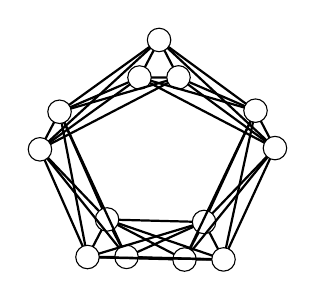
\begin{tikzpicture}[scale = 10]
\tikzstyle{VertexStyle}=[shape = circle,	
								 minimum size = 1pt,
								 inner sep = 3pt,
                         draw]
\Vertex[x = 0.257401078939438, y = 0.729450404644012, L = \tiny {}]{v0}
\Vertex[x = 0.232565611600876, y = 0.681758105754852, L = \tiny {}]{v1}
\Vertex[x = 0.383801102638245, y = 0.820650428533554, L = \tiny {}]{v2}
\Vertex[x = 0.358965694904327, y = 0.772958129644394, L = \tiny {}]{v3}
\Vertex[x = 0.40850430727005, y = 0.773111909627914, L = \tiny {}]{v4}
\Vertex[x = 0.506290018558502, y = 0.730872631072998, L = \tiny {}]{v5}
\Vertex[x = 0.530993163585663, y = 0.683334112167358, L = \tiny {}]{v6}
\Vertex[x = 0.440956592559814, y = 0.589494824409485, L = \tiny {}]{v7}
\Vertex[x = 0.416121125221252, y = 0.541802525520325, L = \tiny {}]{v8}
\Vertex[x = 0.46565979719162, y = 0.541956305503845, L = \tiny {}]{v9}
\Vertex[x = 0.317756593227386, y = 0.592694818973541, L = \tiny {}]{v10}
\Vertex[x = 0.292921125888824, y = 0.545002520084381, L = \tiny {}]{v11}
\Vertex[x = 0.342459797859192, y = 0.545156300067902, L = \tiny {}]{v12}
\Edge[](v1)(v0)
\Edge[](v3)(v2)
\Edge[](v4)(v2)
\Edge[](v4)(v3)
\Edge[](v6)(v5)
\Edge[](v8)(v7)
\Edge[](v9)(v7)
\Edge[](v9)(v8)
\Edge[](v11)(v10)
\Edge[](v12)(v10)
\Edge[](v12)(v11)
\Edge[](v2)(v0)
\Edge[](v3)(v0)
\Edge[](v4)(v0)
\Edge[](v2)(v1)
\Edge[](v3)(v1)
\Edge[](v4)(v1)
\Edge[](v2)(v5)
\Edge[](v3)(v5)
\Edge[](v4)(v5)
\Edge[](v2)(v6)
\Edge[](v3)(v6)
\Edge[](v4)(v6)
\Edge[](v5)(v7)
\Edge[](v6)(v7)
\Edge[](v5)(v9)
\Edge[](v6)(v9)
\Edge[](v5)(v8)
\Edge[](v6)(v8)
\Edge[](v10)(v8)
\Edge[](v11)(v8)
\Edge[](v12)(v8)
\Edge[](v10)(v7)
\Edge[](v11)(v7)
\Edge[](v12)(v7)
\Edge[](v10)(v9)
\Edge[](v11)(v9)
\Edge[](v12)(v9)
\Edge[](v10)(v1)
\Edge[](v11)(v1)
\Edge[](v12)(v1)
\Edge[](v10)(v0)
\Edge[](v11)(v0)
\Edge[](v12)(v0)
\end{tikzpicture}
\caption{The mule $M_{7,2}$.}
\label{fig:M_72}
\end{figure}



\begin{lem}\label{NoForksThatArentKnives}
For $k \geq 7$ and $r \geq 2$, no $k$-mule except $M_{7, 1}$ and $M_{7, 2}$
contains an induced $\join{K_r}{\left(\djunion{K_1}{K_{k - (r + 1)}}\right)}$.
\end{lem}
\begin{proof}
Suppose the lemma is false and let $G$ be a $k$-mule, other than $M_{7,1}$ and
$M_{7,2}$, containing such an induced subgraph $F$ with $r$ maximal. By Lemma
\ref{NoE2} and Lemma \ref{NoTwooks}, the lemma holds for $r \geq k - 3$. So we have $r \leq k - 4$. Now, let $z \in V(F)$ be the vertex with degree $r$
in $F$, $v_1, v_2, \ldots, v_{k - (r + 1)} \in V(F)$ the vertices of degree $k -
2$ in $F$ and $C$ the rest of the vertices in $F$ (all of degree $k-1$ in $F$). Put $H \DefinedAs G - F$.

Let $Z_1 \DefinedAs \setbs{za}{a \in N(v_1) \cap V(H)}$.  
Consider the graph $D \DefinedAs H + z + Z_1$.  
Since $v_1$ has at most two neighbors in $H$, $\card{Z_1} \leq 2$ and thus to
form $D$ from $H + z$, we added $E(A)$ where $A \in \set{K_1, K_2, P_3}$.  Since
$\card{C} \geq 2$, $\Delta(D) \leq k$. Hence Lemma \ref{EpiPower} shows that $H
+ z$ contains a $K_k - E(A)$ or $\chi(D) \leq k - 1$.  
Suppose $\chi(D) \geq k$. 
If $A = K_1$, $A = K_2$, or $A = P_3$, then 
we have a contradiction by the fact that $\omega(G) < k$, Lemma \ref{NoE2}, and
Lemma \ref{NoTwooks}, respectively. Thus
we must have $\chi(D) \leq k - 1$, which gives a $(k - 1)$-coloring of $H + z$
in which $z$ receives a color $c$ which is not received by any of the neighbors
of $v_1$ in $H$. Thus $c$ remains in the list of $v_1$ and we may color $v_1$
with $c$.  After doing so, each vertex in $C$ has a list of size at least $k-3$
and $v_i$ for $i > 1$ has a list of size at least $k-4$.  If any pair of
vertices in $C$ had different lists, then we could complete the partial
coloring by Hall's Theorem.  Let $N \DefinedAs \bigcup_{w \in C} N(w) \cap
V(H)$ and note that $N$ is an independent set since it is contained in a single
color class in the $(k - 1)$-coloring of $H$ just constructed.

Suppose $\card{N} \geq 2$.  Pick $a_1, a_2 \in N$. 
Consider the graph $D \DefinedAs H + z + Z_1 + a_1a_2$.  
Plainly, $\Delta(D) \leq k$. 
To form $D$ from $H + z$ we added $E(A)$, where $A \in \set{K_1, K_2, P_3, K_3,
P_4, \djunion{K_2}{P_3}}$.  Hence Lemma \ref{EpiPower} shows that $H + z$
contains a $K_k - E(A)$ or $\chi(D) \leq k - 1$.  If $\chi(D) \geq k$, then we
have a contradiction since $A = K_1$, $A = K_2$, and $A = P_3$ are impossible
as above.
%
To show that $A=K_3$, $A=P_4$, and $A=\djunion{K_2}{P_3}$ are impossible,
we apply Lemma \ref{NoE3} (this is where we use the fact that
$G\ne M_{7,1}$), Lemma \ref{AJoinP_4} (since $K_t-E(P_4)=\join{P_4}{K_{t-4}}$),
and Lemma \ref{E2Classification}, respectively.
% show the impossibility of $A = K_3$, $A = P_4$ (since
%$K_t-E(P_4)=\join{P_4}{K_{t-4}}$), and $A = \djunion{K_2}{P_3}$ respectively. 

Thus we must have $\chi(D) \leq k - 1$, which gives a $(k -
1)$-coloring of $H + z$ in which $a_1$ and $a_2$ are in different color classes
and $z$ receives a color not received by any neighbor of $v_1$ in $H$.  As
above we can complete this partial coloring to all of $G$ by first coloring $z$
and $v_1$ the same and then using Hall's Theorem.

Hence there is a vertex $x \in V(H)$ which is adjacent to all of $C$.  
Note that $x$ is not adjacent to any of $v_1, v_2, \ldots, v_{k - (r + 1)}$ by the maximality of $r$. 
Let $Z_2 \DefinedAs \setbs{xa}{a \in N(v_2) \cap V(H)}$.  Consider the graph 
$D \DefinedAs H + z + Z_1 + Z_2$.  As above, both $Z_1$ and $Z_2$ have
cardinality at most $2$.  Since $\card{C} \geq 2$, both $x$ and $z$ have degree at most $k$ in $D$.  
Since both $xa$ and $za$ were added only if $a$ was a neighbor of both $v_1$ and $v_2$, 
all the neighbors of $v_1$ in $H$ have degree at most $k$ in $D$. Similarly for $v_2$'s neighbors.  
Hence $\Delta(D) \leq k$. 
To form $D$ from $H + z$ we added $E(A)$ where $A
\in \set{K_1, K_2, P_3, K_3, P_4, \djunion{K_2}{P_3}, 2K_2, P_5, 2P_3, C_4}$. 
Hence Lemma \ref{EpiPower} shows that $H + z$ contains a $K_k - E(A)$ or $\chi(D) \leq k - 1$.  

Suppose $\chi(D) \geq k$. Then $A = K_1$, $A = K_2$, $A = P_3$, $A =
K_3$, $A = P_4$, and $A = \djunion{K_2}{P_3}$ are impossible as above.  
Applying Lemma \ref{E2Classification} shows that $A = 2K_2$, $A = P_5$, and 
$A = 2P_3$ are impossible.  Thus we must have $A = C_4$.  If $k \geq 8$, then 
Lemma \ref{ConnectedAtLeast4Poss} gives a contradiction.  Hence we must have
$k = 7$. 
Since $H + z$ contains an induced $\join{K_3}{2K_2}$, we must have $N(v_1) \cap
V(H) = N(v_2) \cap V(H)$, say $N(v_1) \cap V(H) = \set{w_1, w_2}$.  Moreoever,
$xz \in E(G)$, $w_1w_2 \in E(G)$ and there are no edges between $\set{w_1, w_2}$
and $\set{x, z}$ in $G$.  

Put $Q \DefinedAs \set{v_1, \ldots, v_{k - (r + 1)}}$. Then for $v \in Q$, by
the same argument as above, we must have $N(v) \cap V(H) = \set{w_1, w_2}$. 
Hence $Q$ is joined to $\set{w_1, w_2}$, $C$ is joined to $Q$, and $\set{x, z}$
and both $\set{x, z}$ and $\set{w_1, w_2}$ are joined to the same $K_3$ in $H$. 
We must have $r = 3$ for otherwise one of $x, z, w_1, w_2$ has degree larger
than $7$.  Thus we have an $M_{7, 2}$ in $G$ and therefore $G$ is $M_{7,2}$, a
contradiction.

Thus we must have $\chi(D) \leq k - 1$, which gives a $(k - 1)$-coloring of $H + z$ in which $z$ receives a color $c_1$ which is not received by any of the 
neighbors of $v_1$ in $H$ and $x$ receives a color $c_2$ which is not received by any of the neighbors of $v_2$ in $H$.  
Thus $c_1$ is in $v_1$'s list and $c_2$ is in $v_2$'s list. Note that if $x$ and $z$ are adjacent then $c_1 \neq c_2$. Hence, we can $2$-color $G[x,z,v_1,v_2]$ from the lists.  
This leaves $k-3$ vertices. The vertices in $C$ have lists of size at least $k-3$ and the rest have lists of size at least $k-5$.  
Since the union of any $k-4$ of the lists contains one list of size $k-3$, we
can complete the partial coloring by Hall's Theorem.
\end{proof}

\begin{cor}\label{AtMostOneEdgeIn}
For $k \geq 7$, if $H$ is a $(k - 1)$-clique in a $k$-mule $G$ other than
$M_{7,1}$ and $M_{7,2}$, then any vertex in $G - H$ has at most one neighbor in
$H$.
\end{cor}
\begin{proof}
%Let $S$ denote the vertices of a $(k-1)$-clique, and 
Let $v\notin H$ be adjacent to $r$ vertices in $H$.  Now
$G[H\cup\{v\}]=K_r*(K_1+K_{k-(r+1)})$.  If $r\ge 2$, then $G[H\cup\{v\}]$ is
forbidden by Lemma~\ref{NoForksThatArentKnives}.
\end{proof}

\begin{lem}\label{K4sOut}
For $k \geq 7$, no $k$-mule except $M_{7,1}$ contains
$\join{K_4}{E_{k-4}}$ as a subgraph.
\end{lem}
\begin{proof}
Let $G$ be a $k$-mule other than $M_{7,1}$ and suppose $G$
contains an induced $\join{K_4}{D}$ where $\card{D} = k - 4$. Then $G$ is not
$M_{7,2}$. By Lemma \ref{K_tClassification}, $D$ is $E_3$, a claw, a clique, or
almost complete. If $D$ is a clique then $G$  contains $K_k$, a contradiction. Now Corollary \ref{AtMostOneEdgeIn} shows that $D$ being almost complete is
impossible. Finally, Lemma \ref{NoE3} shows that $D$ cannot be $E_3$ or a claw.  This contradiction completes the proof.
\end{proof}

Since $\join{K_4}{E_{\Delta - 4}} \subseteq K_\Delta$, Lemma \ref{K4sOut} shows that the following conjecture is equivalent to the Borodin-Kostochka conjecture.

\begin{conjecture}\label{K4Conjecture}
Any graph with $\chi \geq \Delta \geq 9$ contains $\join{K_4}{E_{\Delta - 4}}$ as a subgraph.
\end{conjecture}

\begin{lem}\label{NonInducedFourDealInMule}
Let $G$ be a $k$-mule with $k \geq 8$. Let $A$ and $B$ be graphs with $4 \leq \card{A} \leq k - 4$ and $\card{B} = k - \card{A}$ such that $\join{A}{B} \unlhd G$. 
Then $A = \djunion{K_1}{K_{\card{A} - 1}}$ and $B = \djunion{K_1}{K_{\card{B} - 1}}$.
\end{lem}
\begin{proof}
Note that $\card{B} \geq 4$. 
By Lemma \ref{BothSidesAtLeastFourD1Choose}, $\join{A}{B}$ is almost complete, $\join{K_5}{E_3}$ or our desired conclusion holds.  
The first and second cases are impossible by Corollary \ref{AtMostOneEdgeIn} and
Lemma \ref{NoE3}.
\end{proof}

This shows that the following conjecture is a natural weakening of Borodin-Kostochka.

\begin{conjecture}\label{NonInducedFourDeal}
Let $G$ be a graph with $\Delta(G) = k \geq 9$. If $K_{t, k - t} \not \subseteq G$ for all $4 \leq t \leq k - 4$, then $G$ can be $(k - 1)$-colored.
\end{conjecture}

In the next section we create the tools needed to reduce the $4$ in these lemmata to $3$.

\subsection{Tooling up}
For an independent set $I$ in a graph $G$, we write $\frac{G}{\brackets{I}}$ for
the graph formed by collapsing $I$ to a single vertex and discarding duplicate
edges.  We write $\brackets{I}$ for the resulting vertex in the new graph.  If
more than one independent set $I_1, I_2, \ldots, I_m$ are collapsed in
succession we indicate the resulting graph by
$\frac{G}{\brackets{I_1}\brackets{I_2}\cdots\brackets{I_m}}$.

\begin{lem}\label{ToolOne}
Let $G$ be a $k$-mule other than $M_{7,1}$ and $M_{7,2}$ with $k \geq 7$ and $H
\lhd G$. If $x, y \in V(H)$, $xy \not \in E(H)$ and  $\card{N_H(x) \cup N_H(y)} \leq k$, then there exists a $(k - 1)$-coloring $\pi$ of $H$ such that $\pi(x) = \pi(y)$.
\end{lem}
\begin{proof}
Suppose $x, y \in V(H)$, $xy \not \in E(H)$ and $\card{N_H(x) \cup N_H(y)} \leq
k$.  Put $H' \DefinedAs \frac{H}{\brackets{x, y}}$. Then
$H' \prec H$ via the natural epimorphism $\funcsurj{f}{H}{H'}$.  By applying
Lemma \ref{EpiPower} we either get the desired $(k - 1)$-coloring $\pi$ of
$H$ or a $K_{k-1}$ in $H$ with $V(K_{k-1}) \subseteq N(x) \cup N(y)$.  But $k -
1 \geq 6$, so one of $x$ or $y$ has at least three neighbors in $K_{k-1}$
violating Corollary \ref{AtMostOneEdgeIn}.
\end{proof}

\begin{lem}\label{ToolTwo}
Let $G$ be a $k$-mule other than $M_{7,1}$ and $M_{7,2}$ with $k \geq 7$ and $H
\lhd G$.  Suppose there are disjoint nonadjacent pairs $\set{x_1, y_1},
\set{x_2, y_2} \subseteq V(H)$ with $d_H(x_1), d_H(y_1) \leq k - 1$ and $\card{N_H(x_2)
\cup N_H(y_2)} \leq k$. Then there exists a $(k - 1)$-coloring $\pi$ of $H$
such that $\pi(x_1) \neq \pi(y_1)$ and $\pi(x_2) = \pi(y_2)$.
\end{lem}
\begin{proof}
Put $H' \DefinedAs \frac{H}{\brackets{x_2, y_2}} + x_1y_1$.  Then
$H' \prec H$ via the natural epimorphism $\funcsurj{f}{H}{H'}$.  
Suppose the desired $(k - 1)$-coloring $\pi$ of $H$ doesn't exist. 
Apply Lemma \ref{EpiPower} to get a $K_k$ in $H'$. Put $z \DefinedAs
\brackets{x_2, y_2}$.  By Lemma \ref{NoE2} the $K_k$ must contain $z$ and by
Lemma \ref{NoForksThatArentKnives}, the $K_k$ must contain $x_1y_1$; hence
the $K_k$ contains $x_1$, $y_1$, and $z$.  Thus
$H$ contains an induced subgraph $A \DefinedAs \join{\set{x_1, y_1}}{K_{k-3}}$
where $V(A) \subseteq N_H(x_2) \cup N_H(y_2)$.  Then $x_2$ and $y_2$ each have at most
two neighbors in the $K_{k-3}$ by Lemma \ref{K4sOut} and Lemma
\ref{ConnectedEqual3Poss}.  Thus $k=7$ and both $x_2$ and $y_2$ have exactly
two neighbors in the $K_4$.  One of $x_2$ or $y_2$ has at least one neighbor in
$\set{x_1, y_1}$, so by symmetry we may assume that $x_2$ is adjacent to $x_1$. 
But then $\set{x_2} \cup V(A)$ induces either a $\join{K_2}{\text{antichair}}$ (if
$x_2\not\leftrightarrow y_1$) or a graph containing $\join{K_2}{C_4}$ (if
$x_2\leftrightarrow y_1$), and both are impossible by Lemma
\ref{K2ClassificationHelper}.
\end{proof}

\subsection{Using our new tools}

\begin{figure}[htb]
\centering
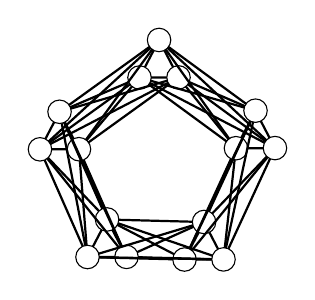
\begin{tikzpicture}[scale = 10]
\tikzstyle{VertexStyle}=[shape = circle,	
								 minimum size = 1pt,
								 inner sep = 3pt,
                         draw]
\Vertex[x = 0.257401078939438, y = 0.729450404644012, L = \tiny {}]{v0}
\Vertex[x = 0.232565611600876, y = 0.681758105754852, L = \tiny {}]{v1}
\Vertex[x = 0.282104313373566, y = 0.681911885738373, L = \tiny {}]{v2}
\Vertex[x = 0.383801102638245, y = 0.820650428533554, L = \tiny {}]{v3}
\Vertex[x = 0.358965694904327, y = 0.772958129644394, L = \tiny {}]{v4}
\Vertex[x = 0.40850430727005, y = 0.773111909627914, L = \tiny {}]{v5}
\Vertex[x = 0.506290018558502, y = 0.730872631072998, L = \tiny {}]{v6}
\Vertex[x = 0.48145455121994, y = 0.683180332183838, L = \tiny {}]{v7}
\Vertex[x = 0.530993163585663, y = 0.683334112167358, L = \tiny {}]{v8}
\Vertex[x = 0.440956592559814, y = 0.589494824409485, L = \tiny {}]{v9}
\Vertex[x = 0.416121125221252, y = 0.541802525520325, L = \tiny {}]{v10}
\Vertex[x = 0.46565979719162, y = 0.541956305503845, L = \tiny {}]{v11}
\Vertex[x = 0.317756593227386, y = 0.592694818973541, L = \tiny {}]{v12}
\Vertex[x = 0.292921125888824, y = 0.545002520084381, L = \tiny {}]{v13}
\Vertex[x = 0.342459797859192, y = 0.545156300067902, L = \tiny {}]{v14}
\Edge[](v2)(v1)
\Edge[](v2)(v0)
\Edge[](v1)(v0)
\Edge[](v4)(v3)
\Edge[](v5)(v3)
\Edge[](v5)(v4)
\Edge[](v7)(v6)
\Edge[](v8)(v6)
\Edge[](v8)(v7)
\Edge[](v10)(v9)
\Edge[](v11)(v9)
\Edge[](v11)(v10)
\Edge[](v13)(v12)
\Edge[](v14)(v12)
\Edge[](v14)(v13)
\Edge[](v3)(v0)
\Edge[](v4)(v0)
\Edge[](v5)(v0)
\Edge[](v3)(v2)
\Edge[](v4)(v2)
\Edge[](v5)(v2)
\Edge[](v3)(v1)
\Edge[](v4)(v1)
\Edge[](v5)(v1)
\Edge[](v3)(v6)
\Edge[](v4)(v6)
\Edge[](v5)(v6)
\Edge[](v3)(v7)
\Edge[](v4)(v7)
\Edge[](v5)(v7)
\Edge[](v3)(v8)
\Edge[](v4)(v8)
\Edge[](v5)(v8)
\Edge[](v6)(v9)
\Edge[](v7)(v9)
\Edge[](v8)(v9)
\Edge[](v6)(v11)
\Edge[](v7)(v11)
\Edge[](v8)(v11)
\Edge[](v6)(v10)
\Edge[](v7)(v10)
\Edge[](v8)(v10)
\Edge[](v12)(v10)
\Edge[](v13)(v10)
\Edge[](v14)(v10)
\Edge[](v12)(v9)
\Edge[](v13)(v9)
\Edge[](v14)(v9)
\Edge[](v12)(v11)
\Edge[](v13)(v11)
\Edge[](v14)(v11)
\Edge[](v12)(v2)
\Edge[](v13)(v2)
\Edge[](v14)(v2)
\Edge[](v12)(v1)
\Edge[](v13)(v1)
\Edge[](v14)(v1)
\Edge[](v12)(v0)
\Edge[](v13)(v0)
\Edge[](v14)(v0)
\end{tikzpicture}
\caption{The mule $M_8$.}
\label{fig:M_8}
\end{figure}


\begin{lem}\label{K3sOut}
For $k \geq 7$, the only $k$-mules containing $\join{K_3}{E_{k-3}}$
as a subgraph are $M_{7,1}$,  $M_{7,2}$ and $M_8$.
\end{lem}
\begin{proof}
Suppose not and let $G$ be a $k$-mule other than $M_{7,1}$,  $M_{7,2}$ and $M_8$
containing $F \DefinedAs \join{C}{B}$ as an induced subgraph where $C
= K_3$ and $B$ is an arbitrary graph with $\card{B} = k - 3$. By Lemma
\ref{ConnectedEqual3Poss}, $B$ is: $\join{E_3}{K_{\card{B} - 3}}$, almost
complete, $\djunion{K_t}{K_{\card{B} - t}}$,
$\djunion{\djunion{K_1}{K_t}}{K_{\card{B} - t - 1}}$, or
$\djunion{E_3}{K_{\card{B} - 3}}$.  The first two options are impossible by
Lemma \ref{K4sOut}.

First, suppose there is no $z \in V(G-F)$ with $C \subseteq N(z)$.  Let $\pi$
be the $(k-1)$-coloring of $G-F$ guaranteed by Lemma
\ref{JoinerOrDifferentLists}.  Put $L \DefinedAs L_\pi$. Let $I$ be a maximal
independent set in $B$. If there are $x,y \in I$ and $c \in L(x) \cap L(y)$,
then we may color $x$ and $y$ with $c$ and then greedily complete the coloring to the rest of $F$ giving a contradiction.  Thus
we must have

\begin{align*}
k - 1 &\geq \sum_{v \in I} \card{L(v)} \\
& \geq \sum_{v \in I} \parens{d_F(v) - 1} \\
&= \sum_{v \in I}(d_B(v) + 3 - 1)\\
&= 2 \card{I} + \sum_{v \in I} d_B(v) \\
&= \card{B} + \card{I} \\
&= k-3 + \card{I}. \\
\end{align*}
Therefore $\card{I} \leq 2$ and hence $B$ is $\djunion{K_t}{K_{\card{B} - t}}$. 
Put $N \DefinedAs \bigcup_{w \in C} N(w) \cap V(G-F)$.  Then $\card{N} \geq 2$
by assumption.  Pick $x_1,y_1 \in N$ and nonadjacent $x_2, y_2 \in V(B)$ and put
$H \DefinedAs G\brackets{V(G-F) \cup \set{x_2, y_2}}$.  Plainly, the conditions
of Lemma \ref{ToolTwo} are satisfied and hence we have a $(k - 1)$-coloring
$\gamma$ of $H$ such that $\gamma(x_1) \neq \gamma(y_1)$ and $\gamma(x_2) =
\gamma(y_2)$.  But then we can greedily complete this coloring to all of $G$, a
contradiction.

Thus we have $z \in V(G-F)$ with $C \subseteq N(z)$.  Put $B' \DefinedAs
G\brackets{V(B) \cup \set{z}}$ and $F' \DefinedAs
G\brackets{V(F) \cup \set{z}}$.  As above, using Lemma
\ref{ConnectedEqual3Poss} and Lemma \ref{K4sOut}, we see that $B'$ is
$\djunion{K_t}{K_{\card{B'} - t}}$, $\djunion{\djunion{K_1}{K_t}}{K_{\card{B'} -
t - 1}}$ or $\djunion{E_3}{K_{\card{B'} - 3}}$.  

Suppose $B'$ is $\djunion{E_3}{K_{\card{B'} - 3}}$, say the $E_3$ is
$\set{z_1, z_2, z_3}$.  Since $k \geq 7$, we have $w_1, w_2 \in V(B') -
\set{z_1, z_2, z_3}$. Then $d_{F'}(z_3) + d_{F'}(w_1) = k$ and hence we may
apply Lemma \ref{ToolOne} to get a $(k - 1)$-coloring $\zeta$ of $G - F'$ such
that there is some $c \in L_\zeta(z_3) \cap L_\zeta(w_1)$.  Now $\card{L_\zeta(z_1)} +
\card{L_\zeta(z_2)} + \card{L_\zeta(w_2)} \geq 2 + 2 + k - 4 = k$ and hence
there is a color $c_1$ that is in at least two of 
$L_\zeta(z_1)$, $L_\zeta(z_2)$ and $L_\zeta(w_2)$.  If $c_1 = c$, then $c$
appears on an independent set of size $3$ in $B'$ and we may color this set
with $c$ and greedily complete the coloring. Otherwise, $B'$ contains two
disjoint nonadjacent pairs which we can color with different colors and again
complete the coloring greedily, a contradiction.

Now suppose $B'$ is $\djunion{\djunion{K_1}{K_t}}{K_{\card{B'} -
t - 1}}$.  By Lemma \ref{NoForksThatArentKnives}, we must have $2 \leq t \leq
\card{B'} - 3$. Let $x$ be the vertex in the $K_1$, $w_1, w_2 \in V(K_t)$ and
$z_1, z_2 \in V(K_{\card{B'} - t - 1})$.  Then $d_{F'}(w_1) + d_{F'}(z_1) = k
+ 1$ and hence we may apply Lemma \ref{ToolOne} to get a $(k - 1)$-coloring
$\zeta$ of $G - F'$ such that there is some $c \in L_\zeta(w_1) \cap
L_\zeta(z_1)$.  Now $\card{L_\zeta(x)} +
\card{L_\zeta(w_2)} + \card{L_\zeta(z_2)} \geq 2 + k-1 = k+1$ and hence
there is are at least two colors $c_1, c_2$ that are each in at least two of 
$L_\zeta(x)$, $L_\zeta(w_2)$ and $L_\zeta(z_2)$.  If $c_1 \neq c$ or $c_2 \neq
c$, then $B'$ contains two
disjoint nonadjacent pairs which we can color with different colors and
then complete the coloring greedily.  Otherwise $c$
appears on an independent set of size $3$ in $B'$ and we may color this set
with $c$ and greedily complete the coloring, a contradiction.

Therefore $B'$ must be $\djunion{K_t}{K_{\card{B'} - t}}$.  
By Lemma \ref{NoForksThatArentKnives}, we must have $3 \leq t \leq \card{B'} -
3$.  Thus $k \geq 8$.  Let $X$ and $Y$ be the two cliques covering $B'$.  Let
$x_1, x_2 \in X$ and $y_1, y_2 \in Y$.  Put $H \DefinedAs G\brackets{V(G-F')
\cup \set{x_1, x_2, y_1, y_2}}$ and $H' \DefinedAs \frac{H}{\brackets{x_1,
y_1}\brackets{x_2,y_2}}$.  For $i \in \irange{2}$, $d_{F'}(x_i) + d_{F'}(y_i) =
k + 2$ and thus $\Delta(H') \leq k$. If $\chi(H') \leq k - 1$, then we have a
$(k-1)$-coloring of $H$ which can be greedily completed to all of $G$, a contradiction.  
Hence, by Lemma \ref{EpiPower}, $H'$ contains $K_k$.  Thence $H - \set{x_1,
y_1, x_2, y_2}$ contains a $K_{k-2}$, call it $A$, such that $V(A) \subseteq
N(x_i) \cup N(y_i)$ for $i \in \irange{2}$.  
%By considering degrees, 
Since $d_{F'}(x_i)+d_{F'}(y_i)=k+2$, we see that
$N_H(x_i) \cap N_H(y_i) = \emptyset$ for $i \in \irange{2}$.  But we can play
the same game with the pairs $\set{x_1, y_2}$ and $\set{x_2, y_1}$.  We conclude
that $N(x_1) \cap V(A) = N(x_2) \cap V(A)$ and $N(y_1) \cap V(A) = N(y_2) \cap
V(A)$.  In fact we can extend this equality to all of $X$ and $Y$.  Put $Q
\DefinedAs N(x_1) \cap V(A)$ and $P \DefinedAs N(y_1) \cap V(A)$.  Then we
conclude that $X$ is joined to $Q$ and $Y$ is joined to $P$.  Moreover, we
already know that $X$ and $Y$ are joined to the same $K_3$.  The edges in these
joins exhaust the degrees of all the vertices, hence $G$ is a $5$-cycle with
vertices blown up to cliques.  If $k = 8$, then $\card{X} = \card{Y} = 3$ and
thus $\card{Q} = \card{P} = 3$, but then $G = M_8$, a contradiction.  So $k
\geq 9$.  Since $\card{X}+\card{Y}= k-2 \ge 7$, we have either $\card{X}\ge 4$
or $\card{Y}\ge 4$.
If $\card{X}\ge 4$, then for each $q\in Q$, we have $d(q)\ge
(k-2)-1+\card{X}\ge k+1$, contradiction.  If $\card{Y}\ge 4$, then for each
$p\in P$, we have $d(p)\ge (k-2)-1+\card{Y}\ge k+1$, contradiction.
\end{proof}

Since $\join{K_3}{E_{\Delta-3}} \subseteq K_\Delta$, Lemma \ref{K3sOut} shows
that Conjecture \ref{K3Conjecture} is equivalent to the Borodin-Kostochka
conjecture.

\begin{lem}\label{NonInducedThreeDealInMule}
Let $G$ be a $k$-mule with $k \geq 7$ other than $M_{7,1}$, $M_{7,2}$ and $M_8$. 
Let $A$ and $B$ be graphs with $3 \leq \card{A} \leq k - 3$ and $\card{B} = k - \card{A}$ such that $\join{A}{B} \unlhd G$. 
Then $A = \djunion{K_1}{K_{\card{A} - 1}}$ and $B = \djunion{K_1}{K_{\card{B} - 1}}$.
\end{lem}
\begin{proof}
Suppose the lemma is false and let $\join{A}{B} \unlhd G$ be a counterexample.

First suppose $\card{A}, \card{B} \geq 4$. 
Then, by Lemma \ref{BothSidesAtLeastFourD1Choose}, $\join{A}{B}$ is almost
complete or $\join{K_5}{E_3}$. The first and
second cases are impossible by Corollary \ref{AtMostOneEdgeIn} and Lemma
\ref{NoE3} respectively.

Thus we may assume $\card{A} = 3$.  By Lemma \ref{K3sOut}, $A \in \set{E_3,
P_3, \djunion{K_1}{K_2}}$.  If $A = E_3$, then $B$ is complete by Lemma
\ref{E3Classification}, but this is impossible by Lemma \ref{NoE3}.  If $A =
P_3$, then $B$ is complete by Lemma \ref{ConnectedIncompleteAtLeast4}, but this
is impossible by Lemma \ref{NoE2}.  Hence $A = \djunion{K_1}{K_2}$.  By Lemma
\ref{AntiP3Classification}, $B$ is complete or $\djunion{K_1}{K_{\card{B} -
1}}$.  The former is impossible by Lemma \ref{NoTwooks} and the latter by
supposition.
\end{proof}

Lemma~\ref{NonInducedThreeDealInMule} proves our main result, that Conjecture
\ref{NoThreeDealEquiv} is equivalent to the Borodin-Kostochka conjecture. 

\subsection{The low vertex subgraph of a mule}
In this section we show that if a mule is not regular, then the subgraph of
non-maximum-degree vertices is severely restricted. For a vertex critical graph
$G$ we write $\fancy{L}(G)$ for the subgraph induced on the vertices of degree $\chi(G) - 1$ in $G$ and $\fancy{H}(G)$ for the subgraph induced on the rest of the vertices.  We call $v \in V(G)$ \emph{low} if $v \in V(\fancy{L}(G))$ and \emph{high} otherwise.

\begin{lem}\label{NoE2InSomeLow}
For $k \geq 6$, no $k$-mule contains an induced $\join{E_2}{K_{k-2}}$ with some
vertex low.
\end{lem}
\begin{proof}
Since $M_{6,1}$ and $M_{7,1}$ contain no such induced subgraph, the lemma
follows from Lemma \ref{NoE2}.
\end{proof}

\begin{lem}\label{LowVerticesAreClique}
If $G$ is a $k$-mule with $k \geq 6$, then $\fancy{L}(G)$ is complete.
\end{lem}
\begin{proof}
Let $G$ be a $k$-mule with $k \geq 6$ and suppose $G$ has nonadjacent low
vertices $x$ and $y$. Then $G + xy \prec G$ and hence, by Lemma \ref{EpiPower}, $G + xy$ contains a $K_k$.  
But then $G$ contains an $\join{E_2}{K_{k-2}}$ with some vertex low, contradicting Lemma \ref{NoE2InSomeLow}.  
Hence $\fancy{L}(G)$ is complete.
\end{proof}

\begin{lem}\label{LowVerticesAreFew}
If $G$ is a $k$-mule with $k \geq 6$ other than $M_{6,1}$ and $M_{7,1}$, then
$\card{\fancy{L}(G)} \leq k - 2$.
\end{lem}
\begin{proof}
Let $G$ be a $k$-mule with $k \geq 6$ other than $M_{6,1}$ and $M_{7,1}$.  
By Lemma \ref{LowVerticesAreClique}, $\fancy{L}(G)$ is complete and hence $\card{\fancy{L}(G)} \leq k - 1$.  
Suppose $\card{\fancy{L}(G)} = k - 1$.  
Since $G$ doesn't contain $K_k$, no high $z$ is adjacent to all of $\fancy{L}(G)$.  
Hence, by Lemma \ref{JoinerOrDifferentLists}, there is a $(k - 1)$-coloring of $\fancy{H}(G)$ that we can complete to all of $G$ using Hall's Theorem.  
This contradiction completes the proof.
\end{proof}

\begin{lem}\label{AtMostTwoIntoLowMule}
Let $G$ be a $k$-mule with $k \geq 6$.  If a high $x \in V(G)$ has at least
three low neighbors, then $x$ is adjacent to all low vertices in $G$.
\end{lem}
\begin{proof}
Assume the lemma is false.
Let $x$ be a high degree vertex with at least three neighbors in
$V(\fancy{L}(G))$.  If $|V(\fancy{L}(G))|=3$, then the claim holds.  So assume
that $|V(\fancy{L}(G))|\ge 4$ and choose $y\in V(\fancy{L}(G))\setminus N(x)$. 
Let $A=V(\fancy{L}(G))\cap N(x)$.  By Lemma \ref{LowVerticesAreClique},
$\fancy{L}(G)$ is complete.  Thus, $G[\{x,y\}\cup A]=\join{E_2}{K_{|A|}}$. 
Since $L(v)=d(v)$ for all $v\in (A\cup\{y\})$, Lemma
\ref{E2JoinWithSomeLowOnBoth} implies that $\join{E_2}{K_{|A|}}$ cannot appear
in $G$.  This contradiction implies the lemma.
\end{proof}

\subsection{Restrictions on the independence number}
The Borodin-Kostochka conjecture has been proven for graphs with independence
number at most two \cite{beutelspacher1984minimal}.  Here we prove that if we
wish to prove the Borodin-Kostochka conjecture for graphs with independence
number at most $a$ for any $a \leq 6$, it suffices to construct a $K_{\Delta
- 1}$.

For $a \geq 2$, let $\fancy{C}_k^a$ be those $G \in \fancy{C}_k$ with $\alpha(G)
\leq a$.  By a $(k,a)$-mule we mean a $\fancy{C}_k^a$-mule. Note that if $G \in
\fancy{C}_k^a$ and for some $H \in \fancy{C}_k$ we have $H \prec G$, then $H \in \fancy{C}_k^a$ as well.
Therefore any $(k,a)$-mule is also a $k$-mule.

\begin{thm}\label{SmallAlphaConj}
For $k \geq 7$ and $2 \leq a \leq k-3$, no $(k, a)$-mule except $M_{7,1}$
contains a $K_{k-1}$.
\end{thm}
\begin{proof}
Suppose otherwise and let $G$ be such a $(k, a)$-mule containing a $K_{k-1}$,
call it $H$. By Corollary \ref{AtMostOneEdgeIn}, each vertex in $G-H$ has at
most one neighbor in $H$.  Let $\pi$ be a $(k-1)$-coloring of $G-H$.  
Then $\card{L_\pi(v)} \geq k - 3$ for all $v \in V(H)$. Since
$H$ cannot be colored from $L_\pi$, applying Hall's Theorem shows that either
$\card{Pot(L_\pi)} \leq k - 2$ or there is some $x \in V(H)$ such that
$\card{Pot_{H-x}(L_\pi)} \leq k - 3$.  In the former case, $\pi$ must have some
color class to which each vertex of $H$ is adjacent and hence $\alpha(G) \geq
k-1$, a contradiction.  In the latter case, $\pi$ must have two color classes to
which each vertex of $H-x$ is adjacent and hence $G$ has two disjoint
independent sets of size $k-2$.  Again we have a contradiction since $\alpha(G)
\geq k-2$.
\end{proof}
It follows that Conjecture \ref{AlphaConjecture} is equivalent to the
Borodin-Kostochka conjecture for graphs with independence number at most $6$.


\chapter{STRONG COLORING}\label{StrongColoringChapter}

Using ideas developed for strong coloring by Haxell \cite{haxell2004strong} and by Aharoni, Berger and Ziv \cite{aharoni2007independent}, we make explicit a recoloring technique and apply it to the Borodin-Kostochka conjecture.

\section{Strong coloring}
For a positive integer $r$, a graph $G$ with $\card{G} = rk$ is called \emph{strongly $r$-colorable} if for every partition of $V(G)$ into parts of size $r$ there is a proper coloring of $G$ that uses all $r$ colors on each part.  If $\card{G}$ is not a multiple of $r$, then $G$ is strongly $r$-colorable iff the graph formed by adding $r\ceil{\frac{|G|}{r}} - |G|$ isolated vertices to $G$ is strongly $r$-colorable.  The \emph{strong chromatic number} $s\chi(G)$ is the smallest $r$ for which $G$ is strongly $r$-colorable.

Note that a strong $r$-coloring of $G$ with respect to a partition $V_1, \ldots, V_k$ of $V(G)$ with $\card{V_i} = r$ must partition $V(G)$ into $r$ independent transversals of $V_1, \ldots, V_k$. In \cite{szabo2006extremal}, Szab{\'o} and Tardos constructed partitioned graphs with part sizes $2\Delta - 1$ that have no independent transversal.  So we must have $s\chi(G) \geq 2\Delta(G)$.  It is conjectured that this bound is tight.

Haxell \cite{haxell2004strong} proved that $s\chi(G) \leq 3\Delta(G) - 1$.  Aharoni, Berger and Ziv \cite{aharoni2007independent} gave a simple proof that $s\chi(G) \leq 3\Delta(G)$.  It is this latter proof whose recoloring technique we use.  First we need a lemma allowing us to pick an independent transversal when one of the sets has only one element.

\begin{lem}\label{SingletonSetTransversal}
Let $H$ be a graph and $V_1 \cup \cdots \cup V_r$ a partition of $V(H)$. 
Suppose that $\card{V_i} \geq 2\Delta(H)$ for each $i \in \irange{r}$.  If a
graph $G$ is formed by attaching a new vertex $x$ to fewer than $2\Delta(H)$
vertices of $H$,  then $G$ has an independent set $\set{x, v_1, \ldots, v_r}$
where $v_i \in V_i$ for each $i \in \irange{r}$.
\end{lem}
\begin{proof}
Suppose not. Remove $\set{x} \cup N(x)$ from $G$ to form $H'$ with induced
partition $V_1', V_2', \ldots, V_r'$. Then $V_1', V_2', \ldots, V_r'$ has no
independent transversal since we could combine one with $x$ to get our desired
independent set in $G$. Note that $\card{V_i'} \geq 1$. 
Create a graph $Q$ by removing edges from $H'$ until it is edge minimal without
an independent transversal. Pick $yz \in E(Q)$ and apply Lemma
\ref{BaseTransversalLemma} on $yz$ with the induced partition to get the guaranteed 
$J \subseteq \irange{r}$ and the totally dominating induced matching 
$M$ with $\card{M} = \card{J} - 1$. 
Now $\card{\bigcup_{i \in J} V_i'} > 2\Delta(H)\card{J} - 2\Delta(H) =
2(\card{J} - 1)\Delta(H)$ and hence $M$ cannot dominate, a contradiction.
\end{proof}


\begin{thm}\label{StrongColorBound}
Every graph satisfies $s\chi \leq 3\Delta$.
\end{thm}
\begin{proof}
We only need to prove that graphs with $n \DefinedAs 3\Delta k$ vertices have a $3\Delta$ coloring for each $k \geq 1$.  
Suppose not and choose a counterexample $G$ minimizing $\size{G}$.  Put $r \DefinedAs 3\Delta(G)$ and let $V_1, \ldots, V_k$ be a partition 
of $G$ for which there is no acceptable coloring.  Then the $V_i$ are independent by minimality of $\size{G}$. By symmetry we may assume 
there are adjacent vertices $x \in V_1$ and $y \in V_2$. Apply minimality of $\size{G}$ to get an $r$-coloring $\pi$ of $G - xy$ 
with $\pi(V_i) = \irange{r}$ for each $i \in \irange{k}$.  We will modify $\pi$ to get such a coloring of $G$.

By symmetry, we may assume that $\pi(x) = \pi(y) = 1$.  For $2 \leq i \leq k$, let $z_i$ be the unique element of $\pi^{-1}(1) \cap V_i$ and 
put 
\[W_i \DefinedAs V_i - \setb{v}{V_i}{\pi(v) = \pi(w) \text{ for some } w \in N(z_i)}.\]  
Then $\card{W_i} \geq 2\Delta(G)$ and we may apply 
Lemma \ref{SingletonSetTransversal} to get a $G$-independent transversal $w_1, w_2, \ldots, w_k$ of $\set{x}, W_2, W_3, \ldots, W_k$.  
Define a new coloring $\zeta$ of $G$ by 


\begin{equation*}
\zeta(v) \DefinedAs 
\begin{cases}
1 & \text{if $v = w_i$} \\
\pi(w_i) & \text{if $v = z_i$} \\
\pi(v) & \text{otherwise.}
\end{cases}
\end{equation*}

\noindent Then $\zeta$ is a proper coloring of $G$ with $\zeta(V_i) = \irange{r}$ for each $i \in \irange{k}$, a contradiction.
\end{proof}

For our application we will need a lopsided version of Lemma \ref{SingletonSetTransversal} Lemma \ref{LopsidedISR}.

\begin{lem}\label{SingletonSetTransversalLopsided}
Let $H$ be a graph and $V_1 \cup \cdots \cup V_r$ a partition of $V(H)$.  
Suppose there exists $t \geq 1$ such that for each $i \in \irange{r}$ and each $v \in V_i$ we have $d(v) \leq \min\set{t, \card{V_i}-t}$.  For any $S \subseteq V(H)$ with $\card{S} < \min\set{\card{V_1}, \ldots, \card{V_r}}$, there is an independent transversal $I$ of $V_1, \ldots, V_r$ with $I \cap S = \emptyset$.
\end{lem}
\begin{proof}
Suppose the lemma fails for such an $S \subseteq V(H)$.  Put $H' \DefinedAs H - S$ and let $V_1', \ldots, V_r'$ be the induced partition of $H'$. Then there is no independent trasversal of $V_1', \ldots, V_r'$ and $\card{V_i'} \geq 1$ for each $i \in \irange{r}$. Create a graph $Q$ by removing edges from $H'$ until it is edge minimal without an independent transversal. Pick $yz \in E(Q)$ and apply Lemma 
\ref{BaseTransversalLemma} on $yz$ with the induced partition to get the guaranteed 
$J \subseteq \irange{r}$ and the tree $T$ with vertex set $J$ and an edge between $a, b \in
J$ for each $uv \in M$ with $u \in V_a'$ and $v \in V_b'$.  By our condition, for each $uv \in E(V_i, V_j)$, we have $\card{N_H(u) \cup N_H(v)} \leq \min\set{\card{V_i}, \card{V_j}}$.

Choose a root $c$ of $T$. Traversing $T$ in leaf-first order and for each leaf $a$ with parent $b$ picking $|V_a|$ from $\min\set{|V_a|, |V_b|}$ we get that the vertices in $M$ together dominate at most $\sum_{i \in J - c} \card{V_i}$ vertices in $H$.  Since $\card{S} < \card{V_c}$, $M$ cannot totally dominate $\bigcup_{i \in J} V_i'$, a contradiction.
\end{proof}

We note that the condition on $S$ can be weakened slightly.  Suppose we have ordered the $V_i$ so that $\card{V_1} \leq \card{V_2} \leq \cdots \leq \card{V_r}$.  Then for any $S \subseteq V(H)$ with $\card{S} < \card{V_2}$ such that $V_1 \not \subseteq S$, there is an independent transversal $I$ of $V_1, \ldots, V_r$ with $I \cap S = \emptyset$.  The proof is the same except when we choose our root $c$, choose it so as to maximize $\card{V_c}$.  Since $\card{J} \geq 2$, we get $\card{V_c} \geq \card{V_2} > \card{S}$ at the end.

\section{The recoloring technique}\label{recolorsection}
We can extract the idea in the proof of Theorem \ref{StrongColorBound} to get a
general recoloring technique.  Suppose $G$ is a $k$-vertex-critical graph and
pick $x \in V(G)$ and $(k-1)$-coloring $\pi$ of $H \DefinedAs G - x$.  Let $Z$
be a color class of $\pi$, say $Z = \pi^{-1}(1)$.  For each $z \in Z$, let
$O_z$ be the neighbors of $z$ which get a color that no other neighbor of $z$ gets; that is, put
$O_z \DefinedAs \setb{v}{N_H(z)}{\pi(v) \not \in \pi(N_H(z) - v)}$.  Suppose the
$O_z$ are pairwise disjoint.  If we could find an independent transversal
$\set{x} \cup \set{v_z}_{z \in Z}$ of $\set{x}$ together with the $O_z$, then
recoloring each $z \in Z$ with $\pi(v_z)$ and coloring each vertex in $\set{x}
\cup \set{v_z}_{z \in Z}$ with $1$ gives a proper $(k-1)$-coloring of $G$.  This
is exactly what happens in the above proof of the strong coloring result.  To
make this work more generally, we need to find situations where each $G[O_z]$
has high minimum degree.  Also, intuitively, the $O_z$ intersecting each other
should make things easier since recoloring a vertex in the intersection of
$O_{z_1}$ and $O_{z_2}$ works for both $z_1$ and $z_2$.  In our application we
will allow some restricted intersections.

\section{A general decomposition}\label{GeneralDecomposition}
Let $\D_1$ be the collection of graphs without induced $d_1$-choosable
subgraphs.  Plainly, $\D_1$ is hereditary. For a graph $G$ and $t \in \IN$, let
$\CC_t$ be the maximal cliques in $G$ having at least $t$ vertices. We prove the
following decomposition result for graphs in $\D_1$ which generalizes Reed's decomposition in \cite{reed1999strengthening}.

\begin{lem}\label{partition}
Suppose $G \in \D_1$ has $\Delta(G) \geq 8$ and contains no $K_{\Delta(G)}$. If
$\frac{\Delta(G) + 5}{2} \leq t \leq \Delta(G) - 1$, then $\bigcup \CC_t$ can be
partitioned into sets $D_1, \ldots, D_r$ such that for each $i \in \irange{r}$
at least one of the following holds:
\begin{itemize}
  \item $D_i = C_i \in \CC_t$,
  \item $D_i = C_i \cup \set{x_i}$ where $C_i \in \CC_t$ and $\card{N(x_i) \cap
  C_i} \geq t-1$.
\end{itemize}

\noindent Moreover, each $v \in V(G) - D_i$ has at most $t-2$ neighbors in $C_i$  for each $i \in \irange{r}$.
\end{lem}
\begin{proof}
Suppose $\card{C_i} \leq \card{C_j}$ and $C_i \cap C_j \neq \emptyset$. 
Then $\card{C_i \cap C_j} \geq \card{C_i} + \card{C_j} - (\Delta + 1) \geq 4$.  It follows from Corollary
\ref{K_tClassification} that $\card{C_i - C_j} \leq 1$.

Now suppose $C_i$ intersects $C_j$ and $C_k$.  By the above,
$\card{C_i \cap C_j} \geq \frac{\Delta(G) + 3}{2}$ and similarly $\card{C_i \cap
C_k} \geq \frac{\Delta(G) + 3}{2}$.  Hence $\card{C_i \cap C_j \cap C_k} \geq
\Delta(G) + 3 - (\Delta(G) - 1) = 4$.  Put $I \DefinedAs C_i \cap C_j \cap C_k$
and $U \DefinedAs C_i \cup C_j \cup C_k$.  By maximality of $C_i, C_j, C_k$,
$U$ cannot induce an almost complete graph.  Thus, by Corollary
\ref{K_tClassification}, $\card{U} \in \set{4, 5}$ and the graph induced on $U -
I$ is $E_3$.  But then $t \leq 6$ and hence $\Delta(G) \leq 7$, a contradiction.

\smallskip

\noindent The existence of the required partition is immediate. 
\end{proof}

\noindent When $D_i \in \CC_t$, we put $K_i \DefinedAs C_i \DefinedAs D_i$ and
when $D_i = C_i \cup \set{x_i}$, we put $K_i \DefinedAs N(x_i) \cap C_i$.

\section{Borodin-Kostochka when every vertex is in a big clique}
Let $G$ be a graph.  For $v \in V(G)$, we let $\omega(v)$ be the size of a
largest clique in $G$ containing $v$.  The proofs of the results in this section
go more smoothly when we strengthen the induction in terms of the parameter
$\rho(G) \DefinedAs \max_{v \in V(G)} d(v) - \omega(v)$.

\begin{thm}
For $k \geq 9$, every graph satisfying $\Delta \leq k$, $\omega < k$ and $\rho
\leq \frac{k}{3} - 2$ is $(k-1)$-colorable.
\end{thm}
\begin{proof}
Suppose the theorem fails for some $k \geq 9$ and choose a counterexample
$G$ minimizing $\card{G} + \size{G}$. Put $\Delta \DefinedAs \Delta(G)$.  If
$\Delta < k$, then $\Delta = k-1$ and by Brooks' theorem $G$ contains $K_k$, a
contradiction. Thus $\chi(G) = k = \Delta$.  Also, for any $v
\in V(G)$ we have $\rho(G-v) \leq \rho(G)$, applying our minimality condition on $G$ implies that $G$ is
vertex critical.

Therefore $\delta(G) \geq \Delta - 1$ and $G \in
\D_1$.  For any $v \in V(G)$, we have $\Delta - 1 - \omega(v) \leq d(v) -
\omega(v) \leq \frac{\Delta}{3} - 2$ and hence $\omega(v) \geq \frac23\Delta +
1$. Applying Lemma \ref{partition} with $t \DefinedAs \frac23\Delta + 1$ we
get a partition $D_1, \ldots, D_r$ of $\bigcup \CC_t = V(G)$.  Note that for $i
\in \irange{r}$, if $K_i \neq D_i$ then all vertices in $K_i$ are high by Lemma
\ref{E2JoinWithSomeLow}.  Pick $x \in K_1$.  Then $x$ has $\card{C_1} - 1 \leq
\Delta - 2$ neighbors in $D_1$ if $K_i = D_i$ and $\card{C_1} \leq \Delta - 1$
if $K_i \neq D_i$.  Hence, by our note, $x$ has a neighbor $w \in V(G) - D_1$.

We now claim that $xw$ is a critical edge in $G$.  Suppose otherwise that
$\chi(G - xw) = \Delta$.  Then by minimality of $G$ we must have $\rho(G-xw) >
\rho(G)$. Hence there is some vertex $v \in N(x) \cap N(w)$ so that every
largest clique containing $v$ contains $xw$.  But $v$ is in some $D_j$ and all largest cliques containing $v$ are contained in $D_j$ and hence do not contain $xw$, a contradiction.  

Let $\pi$ be a $(\Delta-1)$-coloring of $G - xw$ chosen so that $\pi(x) = 1$
and so as to minimize $\card{\pi^{-1}(1)}$. Consider $\pi$ as a coloring of
$G-x$. One key property of $\pi$ we will use is that since $x$ got $1$ in the
coloring of $G - xw$ and $x \in K_1$, no vertex of $D_1 - x$ gets colored $1$ by $\pi$.

Now put $Z \DefinedAs \pi^{-1}(1)$ and for $z \in Z$, let $O_z$ be as defined
in Section \ref{recolorsection}.  By minimality of $\card{Z}$, each $z \in Z$ has at least one neighbor in every color class of $\pi$.  
Hence $z$ has two or more neighbors in at most $2 + d(z) - \Delta$ of
$\pi$'s color classes. For each $z \in Z$ we have $i(z)$ such that $z \in D_{i(z)}$. For $z \in Z$ such that $i(z) \not \in i(Z - z)$, put $V_z \DefinedAs O_z \cap C_{i(z)}$.  

We have $\card{V_z} \geq \omega(z) - 1 - \parens{2 + d(z) - \Delta}$.  Since $\omega(z) \geq d(z) - \frac13 \Delta + 2$, we have $\card{V_z} \geq \frac23 \Delta - 1$.   Each $y \in V_z$ is adjacent to all of $C_{i(z)} - \set{y}$ and hence has at most $d(y) + 1 - \card{C_{i(z)}}$ neighbors outside $D_{i(z)}$.  Since $\omega(y) \geq d(y) +
2 - \frac13 \Delta$, we conclude that $y$ has at most $d(y) + 1
- (d(y) + 2 - \frac13 \Delta) = \frac13 \Delta - 1$ neighbors outside $D_{i(z)}$.

Now let $Z'$ be the $z \in Z$ with $i(z) \in i(Z - z)$. Then $Z'$ can be partitioned into pairs $\set{z, z'}$ such that $i(z) = i(z')$.  For such a pair, one of $z,z'$ is $x_{i(z)}$ and the other is in $C_{i(z)} - K_{i(z)}$. Put $V_z \DefinedAs O_z \cap O_{z'} \cap K_{i(z)}$ and don't define $V_{z'}$.  We have $\card{V_z} \geq \min\set{\omega(z), \omega(z')} - 1 - \parens{2 + d(z) - \Delta} - \parens{2 + d(z') - \Delta} \geq - \frac13 \Delta + 2 - 1 - 2\parens{2 - \Delta} - \max\set{d(z), d(z')} = \frac53 \Delta - \max\set{d(z), d(z')} - 3 \geq \frac23 \Delta - 3$.  Each $y \in V_z$ is adjacent to all of $D_{i(z)} - \set{y}$ and hence has at most $d(y) + 1 - \card{D_{i(z)}}$ neighbors outside $D_{i(z)}$.  Since $\card{D_{i(z)}} = \omega(y) + 1 \geq d(y) + 3 - \frac13 \Delta$, we conclude that $y$ has at most $\frac13 \Delta - 2$ neighbors outside $D_{i(z)}$.

Let $H$ be the subgraph of $G$ induced on the union of the $V_z$.  Put $S \DefinedAs N(x) \cap V(H)$.  Since $Z \cap D_1 = \emptyset$, $x$ has at least $\card{D_1} - 1$ neighbors in $D_1$ none of which are in $S$.  Hence $\card{S} \leq d(x) + 1 - \card{D_1} \leq d(x) + 1 - \omega(x) \leq \frac{\Delta}{3} - 1 < \card{V_z}$ for all $V_z$ since $\Delta \geq 7$. Hence we may apply Lemma
\ref{SingletonSetTransversalLopsided} on $H$ with $t \DefinedAs \frac13\Delta - 1$ to get an independent set $\set{v_z}_{z\in Z}$ disjoint from $S$ where $v_z \in V_z$. Recoloring each $z \in Z$ with $\pi(z)$ and
coloring $x \cup \set{v_z}_{z \in Z}$ with $1$ gives a $(\Delta - 1)$-coloring
of $G$, a contradiction.
\end{proof}

The following special case is a bit easier to digest.

\begin{cor}\label{TwoThirdsCliqueCor}
Every graph with $\chi \geq \Delta \geq 9$ such that every
vertex is in a clique on $\frac23\Delta + 2$ vertices contains $K_\Delta$.
\end{cor}
\section{Reducing to the irregular case}
It is easy to see that if there are irregular counterexamples to the
Borodin-Kostochka conjecture, then there are regular examples as well: take an
irregular counterexample $G$ clone it add an edge between any vertex with degree
less than $\Delta(G)$ and its clone; repeat until you have a regular graph (from
\cite{molloy2002graph}).

But what about the converse?  If there are regular examples, must there be
(connected) irregular examples?  We'll see that the answer is yes, but we need
to decrease the maximum degree by one.

\begin{thm}\label{IrregularReduction}
Every graph satisfying $\chi \geq \Delta = k \geq 9$ either
contains $K_k$ or contains an irregular critical subgraph satisfying $\chi
= \Delta = k - 1$.
\end{thm}
\begin{proof}
Suppose not and choose a counterexample $G$ minimizing $\card{G}$. Then $G$ is
vertex critical. If every vertex in $G$ were contained in a $(k-1)$-clique, 
then Corollary \ref{TwoThirdsCliqueCor} would give a $K_k$ in $G$, impossible. 
Hence we may pick $v \in V(G)$ not in a $(k-1)$-clique. If $v$ is high, choose a
$(k-1)$-coloring $\pi$ of $G-v$ so that the color class $T$ of $\pi$
where $v$ has two neighbors is as large as possible; if $v$ is low, let $\pi$ be a
$(k-1)$-coloring of $G-v$ where some color class $T$ of $\pi$ is as large as
possible.  By symmetry, we may assume that $\pi(T) = k-1$.  

Now we have a $(k-1)$-coloring $\zeta$ of $H \DefinedAs G-T$ given by $\zeta(x)
= \pi(x)$ for $x \neq v$ and $\zeta(v) = k-1$.  Since $\chi(H) = k - 1$, the
maximality condition on $T$ together with Brooks' theorem gives $\Delta(H) =
k - 1$.  Note that $d_H(v) = k - 2$.  Let $H'$ be a $(k-1)$-critical subgraph of
$H$.  Then $H'$ must contain $v$ and hence is not $K_{k-1}$.  Since $d_{H'}(v) =
k-2$ and $\Delta(H') = k - 1$ (by Brooks' theorem), $H'$ is an irregular
critical subgraph of $G$ satisfying $\chi = \Delta = k - 1$, a contradiction.
\end{proof}

Since the only known critical (or connected even) counterexample to
Borodin-Kostochka for $\Delta = 8$ is regular (see Figure \ref{fig:M_8}) we
might hope that the following strengthened conjecture is true.

\begin{conjecture}\label{EightRegular}
Every critical graph satisfying $\chi \geq \Delta = 8$ is regular.
\end{conjecture}

\section{Dense neighborhoods}
Here we show that the Borodin-Kostochka conjecture holds for graphs where each neighboorhood has ``most'' of its possible edges.  First, we need to convert high average degree in a neighborhood into a large clique in the neighborhood. We need the following extension of a fundamental result of Mader \cite{mader} (see Diestel \cite{diestel2010} for some history of this result).  We will also need $d_1$-choosability results from $\cite{mules}$ as well as some ideas for dealing with average degree in neighborhoods used in \cite{cranstonrabernclaw}.

\begin{lem}\label{MaderLemma}
For $k \geq 1$, every graph $G$ with $d(G) \geq 4k$ has a $(k+1)$-connected induced subgraph $H$ such that $d(H) > d(G) - 2k$.
\end{lem}

\begin{lem}\label{LowVertexHighAverageDegree}
If $B$ is a graph with $d(B) \geq \omega(B) + 2$, then $B$ has an induced subgraph $H$ such that $\join{K_1}{H}$ is $f$-choosable where $f(v) \geq d(v)$ for the $v$ in the $K_1$ and $f(x) \geq d(x) - 1$ for $x \in V(H)$.
\end{lem}
\begin{proof}
Let $B$ be such a graph.  Applying Lemma \ref{MaderLemma} with $k \DefinedAs 1$, we get a $2$-connected subgraph $H$ of $B$ with $d(H) > d(B) - 2 \geq \omega(B)$.  Since $H$ is $2$-connected, if it is not $d_0$-choosable, then it is either an odd cycle or complete.  The former is impossible since $d(H) \geq 3$, hence $H$ would be complete and we'd have the contradiction $\omega(H) > \omega(B)$.  Hence $H$ is $d_0$-choosable.  

Suppose $\join{K_1}{H}$ isn't $f$-choosable and let $L$ be a minimal bad $f$-assignment on $\join{K_1}{B}$.  
By Lemma \ref{LowSinglePair}, no nonadjacent pair in $H$ have intersecting lists and hence we must have $\sum_{v \in V(H)} \card{L(v)} \leq \card{Pot(L)}\omega(H)$.  Since for each $v \in V(H)$ we have $\card{L(v)} \geq d_H(v)$ and by the Small Pot Lemma we have $\card{Pot(L)} \leq \card{H}$, we must have $d(H) \leq \omega(H) \leq \omega(B) < d(H)$, a contradiction.
\end{proof}

\begin{lem}\label{VertexHighAverageDegree}
If $B$ is a graph with $d(B) \geq \omega(B) + 3$, then $B$ has an induced subgraph $H$ such that $\join{K_1}{H}$ is $d_1$-choosable.
\end{lem}
\begin{proof}
Let $B$ be such a graph.  Applying Lemma \ref{MaderLemma} with $k \DefinedAs 1$, we get a $2$-connected subgraph $H$ of $B$ with $d(H) > d(B) - 2 \geq \omega(B) + 1$.  As in the proof of Lemma \ref{LowVertexHighAverageDegree}, we see that $H$ is $d_0$-choosable. Suppose $\join{K_1}{H}$ is not $d_1$-choosable and let $L$ be a minimal bad $d_1$-assignment on $\join{K_1}{H}$.  Combining Lemma \ref{NeighborhoodPotShrink} with the same argument as in the proof of Lemma \ref{LowVertexHighAverageDegree} shows that $\card{Pot(L)} \leq \card{H}-1$.

Now, for $c \in Pot(L)$, we consider how big the color graphs $H_c$ can be.  All of the information comes from Lemma \ref{IntersectionsInB}. We have $\alpha(G_c) \leq 2$ for all $c \in Pot(L)$. First, suppose we have $c \in Pot(L)$ such that $\card{H_c} \geq \omega(H) + 3$.  Then, using Lemma \ref{IntersectionsInB}, we see that $\card{H_{c'}} \leq \omega(H)$ for all $c' \in Pot(L) - c$ and hence $\sum_{\gamma \in Pot(L)} \card{H_\gamma} \leq \card{H} + \parens{\card{Pot(L)} - 1}\omega(H) \leq \card{H}\omega(H) + \card{H} - 2\omega(H)$.  Now suppose we have $c \in Pot(L)$ such that $\card{H_c} = \omega(H) + 2$.  Then, using Lemma \ref{IntersectionsInB} again, we see that $\card{H_{c'}} \leq \omega(H) + 1$ for all $c' \in Pot(L) - c$ and hence $\sum_{\gamma \in Pot(L)} \card{H_\gamma} \leq 1 + \card{Pot(L)}(\omega(H) + 1) \leq \card{H}\omega(H) + \card{H} - \omega(H)$.

Therefore we must have $2\size{H} \leq \card{H}(\omega(H) + 1) - \omega(H)$ and hence $d(H) \leq \omega(H) + 1 < d(H)$, a contradiction.
\end{proof}

\begin{thm}\label{BKdense}
Every graph $G$ with $\omega(G) < \Delta(G)$ such that $d(G_v) \geq \frac23\Delta(G) + 4$ for each $v \in V(G)$ is $(\Delta(G)-1)$-colorable.
\end{thm}
\begin{proof}
Suppose note and let $G$ be a counterexample. Put $\Delta \DefinedAs \Delta(G)$.  Let $H$ be a $\Delta$-vertex-critical induced subgraph of $G$.  Then $\delta(H) \geq \Delta - 1$ and $H$ has no $d_1$-choosable induced subgraphs. By Theorem \ref{TwoThirdsCliqueCor}, we must have $v \in V(H)$ with $\omega(v) < \frac23\Delta + 2$. Suppose $d(H_v) < d(G_v)$. Then $d_H(v) = \Delta - 1$ and $\size{H_v} \geq \size{G_v} - (\Delta - 1)$; therefore, $d(H_v) > d(G_v) - 1 \geq \frac23\Delta + 3$.  Applying Lemma \ref{LowVertexHighAverageDegree} gives $\omega(v) > d(H_v) - 1 \geq \frac23\Delta + 2$, a contradiction.

Hence we must have $d(H_v) = d(G_v) \geq \frac23\Delta + 4$.  Applying Lemma \ref{VertexHighAverageDegree} gives $\omega(v) > d(H_v) - 2 \geq \frac23\Delta + 2$, a contradiction.
\end{proof}

\section{Bounding the order and independence number}
\begin{lem}\label{Onesies}
Let $G$ be a vertex critical graph with $\chi(G) = \Delta(G) + 1 - k$.  For every $v \in V(G)$ there is $H_v \unlhd G_v$ with:
\begin{enumerate}
\item $\card{H_v} \geq \Delta(G) - 2k$; and
\item $\delta(H_v) \geq \card{H_v} - (k+1)(\alpha(G) - 1) - 1$; and
\item $\size{H_v} \geq \card{H_v}\parens{\card{H_v}- (k+2)} - (k+1)\parens{\card{G} + 2k - (\Delta(G) + 1)}$.
\end{enumerate}
\end{lem}
\begin{proof}
Put $\Delta \DefinedAs \Delta(G)$. Pick $v \in V(G)$ and let $\pi$ be a $(\Delta - k)$-coloring of $G-v$.  Let $H_v$ be the subgraph of $G_v$ induced on $\setb{x}{N(v)}{\pi(x) \not \in \pi(N(v) - x)}$.  Plainly, $\card{H_v} \geq \Delta - 2k$.

By the usual Kempe chain argument, any $x, y \in V(H_v)$ must be in the same component of $C_{x,y} \DefinedAs G[\pi^{-1}(\pi(x)) \cup \pi^{-1}(\pi(y))]$.  Thus if $xy \not \in E(G)$, there must be a path of length at least $3$ in $C_{x,y}$ from $x$ to $y$ and hence some vertex of color $\pi(x)$ other than $x$ must have at least two neighbors of color $\pi(y)$ and some vertex of color $\pi(y)$ other than $y$ must have at least two neigbhors of color $\pi(x)$.  We say that such an intermediate vertex \emph{proxies} for $xy$.  Each $xy$ with $y \in V(H_v)$ must have some proxy $z_{xy} \in \pi^{-1}(\pi(x)) - x$ such that $z_{xy}$ proxies for at most $k+1$ total $xw$ with $w \in V(H_v)$, for otherwise we could recolor all of $xy$'s proxies, swap $\pi(x)$ and $\pi(y)$ in $x$'s component of $C_{x,y}$ and then color $v$ with $\pi(x)$ to get a $(\Delta-k)$-coloring of $G$.  We conclude that $x$ has at most $(k+1)(\card{\pi^{-1}(\pi(x))} - 1)$ non-neighbors in $H_v$.  This gives (2) immediately.

For (3), note that $\card{\pi(i)} \geq 2$ for each $i \in \irange{\Delta-k} - \pi(V(H_v))$ and hence $\sum_{j \in \pi(V(H_v))} \card{\pi^{-1}(j)} \leq \card{G} - 1 - 2(\Delta - k - \card{H_v})$.  Since 
\[\size{H_v} \geq \sum_{j  \in \pi(V(H_v))} \parens{\card{H_v} - 1 - (k+1)(\card{\pi^{-1}(j)} - 1)},\] 
\noindent we see that (3) follows.
\end{proof}

\begin{thm}\label{AlphaBound}
Every graph satisfies $\chi \leq \max\set{\omega, \Delta - 1, 4\alpha}$.
\end{thm}
\begin{proof}
Suppose not and choose a counterexample $G$ minimizing $\card{G}$.  Since none of the terms on the right side increase when we remove a vertex, $G$ is vertex critical.  Since the Borodin-Kostochka conjecture holds for graphs with $\alpha = 2$ and $\Delta \geq 9$, we must have $\alpha(G) \geq 3$ and hence $\Delta(G) \geq 13$.  By Lemma \ref{TwoThirdsCliqueCor}, there must be $v \in V(G)$ with $\omega(v) < \frac23 \Delta(G) + 2$.  Applying (2) of Lemma \ref{Onesies}, we get $H_v \unlhd G_v$ with $\card{H_v} \geq \Delta(G) - 2$ and $\delta(H_v) \geq \card{H_v} - 2\alpha(G) + 1$.  Since $\Delta(G) \geq \chi(G) \geq 4\alpha(G) + 1$, we have $\delta(H_v) \geq \card{H_v} - \frac{\Delta(G) - 1}{2} + 1 \geq \frac{\card{H_v} + 1}{2}$.  Applying Lemma \ref{neighborhood} shows that either $H_v = \join{K_3}{E_4}$ or $\omega(H_v) \geq \card{H_v} - 1$.  The former is impossible since $\Delta(G) > 9$. Therefore $\omega(v) \geq \omega(H_v) + 1 \geq \Delta(G) - 2 \geq \frac23 \Delta(G) + 2$ since $\Delta(G) \geq 12$, a contradiction.
\end{proof}

\begin{thm}\label{OrderBound}
Every graph satisfies $\chi \leq \max\set{\omega, \Delta - 1, \ceil{\frac{15 + \sqrt{48n + 73}}{4}}}$.
\end{thm}
\begin{proof}
Suppose not and choose a counterexample $G$ minimizing $\card{G}$.  Put $\Delta \DefinedAs \Delta(G)$ and $n \DefinedAs \card{G}$. Since none of the terms on the right side increase when we remove a vertex, $G$ is vertex critical. By Lemma \ref{TwoThirdsCliqueCor}, there must be $v \in V(G)$ with $\omega(v) < \frac23 \Delta + 2$.  Applying (3) of Lemma \ref{Onesies}, we get $H_v \unlhd G_v$ with with $\card{H_v} \geq \Delta - 2$ and $\size{H_v} \geq \card{H_v}\parens{\card{H_v}- 3} - 2\parens{n + 1 - \Delta}$.  By Lemma \ref{VertexHighAverageDegree}, we must have $d(H_v) < \frac23\Delta + 4$ and hence we have

\begin{align*}
\frac23\Delta + 4 &> 2\parens{\card{H_v}- 3} - \frac{4\parens{n + 1 - \Delta}}{\card{H_v}}\\
&\geq 2\parens{\Delta - 5} - \frac{4\parens{n + 1 - \Delta}}{\Delta - 2}.\\
\end{align*}

Simplifying a bit, we get $6(n-1) > (2\Delta - 15)(\Delta - 2)$.  Since $\Delta \geq \chi(G) \geq \frac{19 + \sqrt{48n + 73}}{4}$, we have $6(n-1) > (\frac{-11 + \sqrt{48n + 73}}{2})(\frac{11 + \sqrt{48n + 73}}{4}) = \frac{48n - 48}{8} = 6(n-1)$, a contradiction.
\end{proof}

\chapter{\texorpdfstring{LIST BORODIN-KOSTOCHKA FOR LARGE $\Delta$}{LIST BORODIN-KOSTOCHKA FOR LARGE MAXIMUM DEGREE}}\label{ChoiceLargeDeltaChapter}
\section{The setup}
\noindent The aim of this chapter is to prove the following result.

\begin{thm}
There exists $\Delta_0$ such that every graph $G$ with $\chi_l(G) \geq \Delta(G)
\geq \Delta_0$ contains a $K_{\Delta(G)}$.
\end{thm}

Suppose the theorem is false and choose a counterexample $G$ minimizing
$\card{G}$.  Put $\Delta \DefinedAs \Delta(G)$ and let $L$ be a bad
$(\Delta - 1)$-assignment on $G$.  Then, by minimality of $\card{G}$, any proper
induced subgraph of $G$ is $L$-colorable.  In particular, every vertex has
degree either $\Delta$ or $\Delta-1$, we call these \emph{high} and \emph{low}
vertices respectively. 

If $G$ had an induced $d_1$-choosable subgraph $H$, then we could
$L$-color $G - H$ by minimality and then complete the $L$-coloring to all of
$G$.  So, $G$ has no $d_1$-choosable induced subgraphs.  

The proof strategy is the same as Reed's \cite{reed1999strengthening} for
chromatic number, except some more care must be taken when lists have small
intersection and $K_{\Delta-1}$'s require special attention.

\section{The decomposition}
We use Lemma \ref{partition} and the notation from Section
\ref{GeneralDecomposition}.

\begin{defn}
The cliques in $\CC_{\frac34 \Delta + 1}$ are called \emph{big}.
\end{defn}

Let $B$ be all vertices contained in a big clique; that is, $B \DefinedAs
\bigcup \CC_{\frac34 \Delta + 1}$. For a vertex $v$, put $G_v \DefinedAs G[N(v)]$.

\begin{defn}
A vertex $v$ is called \emph{sparse} if $\size{G_v} < \frac25 \Delta^2$.
\end{defn}

\begin{lem}\label{neighborhood}
If $B$ is a graph with $\delta(B) \geq \frac{\card{B} + 1}{2}$ such that
$\join{K_1}{B}$ is not $d_1$-choosable, then $\omega(B) \geq \card{B} - 1$ or
$B = \join{E_3}{K_4}$.
\end{lem}
\begin{proof}
Suppose the lemma is false and let $L$ be a minimal bad $d_1$-assignment on $B$.
First note that if $B$ does not contain disjoint nonadjacent pairs $x_1, y_1$
and $x_2, y_2$, then $\omega(B) \geq \card{B} - 1$ or
$B = \join{E_3}{K_4}$ by Corollary \ref{K_tClassification}.

By Dirac's theorem, $B$ is hamiltonian and in particular $2$-connected. Since
$B$ cannot be an odd cycle or complete, $B$ is $d_0$-choosable.

By the Small Pot Lemma, $\card{Pot(L)} \leq \card{B}$.  Since $\card{L(x_1)} +
\card{L(x_2)} \geq \card{B} + 1$, the lists intersect and thus Lemma
\ref{NeighborhoodPotShrink} shows that $\card{Pot(L)} \leq \card{B} - 1$. But
then $\card{L(x_i) \cap L(y_i)} \geq 2$ for each $i$ and Lemma
\ref{IntersectionsInB} gives a contradiction.
\end{proof}

Note that the neighborhoods we will be looking at are huge, so the $B =
\join{E_3}{K_4}$ case will never happen here.

\begin{lem}
Every vertex in $V(G) - B$ is sparse.
\end{lem}
\begin{proof}
Suppose $x \in V(G) - B$.
By applying Lemma \ref{neighborhood} repeatedly, we get a sequence $y_1,
\ldots, y_{\floor{\frac{\Delta}{4}}} \in N(x)$ such that 
\[\card{N(y_i) \cap (N(x) - \set{y_1, \ldots, y_{i-1}})} \leq \frac12 (\Delta +
1 - i).\]

\noindent Hence $x$ is sparse since

\[\size{G_x} \leq \binom{\Delta}{2} -
\frac12\sum_{i=1}^{\floor{\frac{\Delta}{4}}} (\Delta - i) < \frac25 \Delta^2.\]
\end{proof}

\noindent Let $D_1, \ldots, D_r$ be the partition of $B$ guaranteed by Lemma
\ref{partition} and put $S \DefinedAs V(G) - B$.

\section{The random procedure}
For each vertex $v$, pick $c \in L(v)$ at random to get a possibly improper
coloring $\zeta$ of $G$ from $L$.  Put $U \DefinedAs \setb{x}{V(G)}{\zeta(x) =
\zeta(y) \text{ for some $y \in N(x)$}}$.  Put $H \DefinedAs G - U$, $F
\DefinedAs G[U]$ and let $\pi$ be $\zeta$ restricted to $V(H)$.  We refer
to $V(H)$ as the \emph{colored} vertices and $V(F)$ as the \emph{uncolored}
vertices.  Also, let $J$ be the resulting list assignment on $F$; that is, $J(x)
\DefinedAs L(x) - \bigcup_{y \in N(x) \cap V(H)} \pi(y)$ for $x \in V(F)$.

\begin{defn}
A vertex in $v \in V(G)$ is called \emph{safe} if it is colored or $\card{J(v)}
\geq d_F(v) + 1$.
\end{defn}

Note that if every vertex is safe, then we can easily complete the $L$-coloring
to all of $G$.  Our goal will be to show that the random procedure will, with
positive probability, produce a partial coloring where every sparse vertex is
safe and the uncolored nonsparse vertices satisfy conditions that will allow the
coloring to be completed.  Now we make this precise.  Consider the following
events:

\begin{itemize}
  \item $S_v$, for $v \in S$: the event that $v$ is not safe.
  \item $E_i$, for $i \in \irange{r}$ where $\card{C_i} \leq \Delta - 2$: the event that $C_i$ does not contain two uncolored safe vertices.
  \item $Q_i$, for $i \in \irange{r}$ where $\card{C_i} \leq \Delta - 2$: the event that $K_i$ does not contain two uncolored vertices.
  \item $F_i$, for $i \in \irange{r}$ where $\card{C_i} = \Delta - 1$, every $x
  \in G - C_i$ has $\card{N(x) \cap C_i} \leq \sqrt{\Delta}\log(\Delta)$ and
  there are at most $\log^2(\Delta)$ vertices $x \in G - C_i$ with $\card{N(x)
  \cap C_i} > \frac{\sqrt{\Delta}}{\log(\Delta)}$: the event that
  $C_i$ does not contain two uncolored safe vertices.
  \item $P_i$, for $i \in \irange{r}$ where $\card{C_i} = \Delta - 1$ and either some $x \in G
  - C_i$ has $\card{N(x) \cap C_i} > \sqrt{\Delta}\log(\Delta)$ or more than
  $\log^2(\Delta)$ vertices $x \in G - C_i$ have $\card{N(x) \cap C_i} >
  \frac{\sqrt{\Delta}}{\log(\Delta)}$: the event that every $x \in G - C_i$ has
  at most two ``good clumps'' in $K_i$.
\end{itemize}

It remains to define ``good clumps''.  To do so we need a lemma.

\begin{lem}\label{clumping}
Let $K$ be a $\Delta-1$ clique in $G$ and $x \in G - K$ with $\card{N(x) \cap
K} \geq 4$.  Then every vertex in $\card{N(x) \cap
K}$ is high and there is a partition $\set{Z_1, \ldots, Z_m}$
of $N(x) \cap K$ such that for each $i \in \irange{m}$ we have $\card{Z_i} \leq
5$ and $L(u) = L(v)$ for all $u, v \in Z_i$.  Moreover, $\card{L(v) - L(w)}
\leq 1$ for all $v, w \in N(x) \cap K$.
\end{lem}
\begin{proof}
Put $A \DefinedAs N(x) \cap K$ and $Q \DefinedAs G[\set{x} \cup K]$.  For any
$L$-coloring $\gamma$ of $G - Q$, let $L_\gamma$ be the resulting list
assignment on $Q$.

First, suppose there is an $L$-coloring $\gamma$ of $G - Q$ such that
$L_\gamma(u) \neq L_\gamma(v)$ for some $u, v \in A$.  Pick $y \in K - A$.  If
$L_\gamma(x) \cap L_\gamma(y) \neq \emptyset$, then coloring $x$ and $y$ the
same leaves a list assignment on $K - y$  which is completable by Hall's theorem.
Hence we must have $L_\gamma(x) \cap L_\gamma(y) = \emptyset$.  Thus $\card{L_\gamma(x) \cup L_\gamma(y)} \geq \Delta$.  Put $Pot(T) \DefinedAs \bigcup_{v \in T} L_\gamma(v)$ for $T \subseteq A$.  If there is $c \in (L_\gamma(x) \cup L_\gamma(y)) - Pot(A)$, then coloring $x$ and $y$ so that $c$ is used leaves a list assignment on $K-y$ which is completable by Hall's theorem.  In particular, we must have $\card{Pot(A)} \geq \Delta$. Now, if we color $x$ and $y$ arbitrarily we can complete the coloring unless there exists $T \subseteq A$ with $\card{T} = \card{A}-1$ and $\card{Pot(T)} \leq \Delta - 2$.  Thus we can pick a color in $L_\gamma(x) \cup L_\gamma(y)$ which is not in any of $T$'s lists giving a coloring that is again easily completable.

Therefore $L_\gamma(u) = L_\gamma(v)$ for all $u, v \in A$ for every
$L$-coloring $\gamma$ of $G - Q$.  In particular, no vertex of $A$ is
low and $\card{L(v) - L(w)} \leq 1$ for all $v, w \in A$.  Suppose there exists
$Z \subseteq A$ with $\card{Z} \geq 6$ such that $L(u) = L(v)$ for all $u, v \in Z$.  Then every $v
\in Z$ has exactly one neighbor $z_v$ in $G-Q$.  Put $N \DefinedAs
\setbs{z_v}{v \in Z}$.  If $\card{N} = 1$, then $G$ contains $\join{K_6}{E_3}$
violating Lemma \ref{K_tClassification}.  If some $L$-coloring $\gamma$ of $G-Q$ assigned
two vertices of $N$ different colors, then $L_\gamma$ would give different lists
for two vertices of $A$, a contradiction.  Hence $N$ is an independent set and
adding an edge between two vertices of $N$ in $G-Q$ must create a $K_\Delta$ by
minimality of $\card{G}$.  By counting degrees this is plainly impossible for
$\card{N} \geq 3$.  For $\card{N} = 2$, both vertices have $\Delta-2$ neighbors
in $G-Q$ and one has at least $3$ vertices in $Z$, impossible.

Now taking maximal subsets of $A$ of vertices all having the same list gives the
desired partition.
\end{proof}

The $Z_i$ in the partition in Lemma \ref{clumping} are called \emph{clumps} of $x$ in $K$.
Note that there exists $Y$ such that for any $i \neq j$ we have $L(v) \cap L(z)
= Y$ for $v \in Z_i$ and $w \in Z_j$.  For $i \in \irange{m}$ and $v \in Z_i$ we
let $\alpha_i$ be the unique element of $L(v) - Y$.  We call $\alpha_i$ the
\emph{special} color for $Z_i$.

Now let $i \in \irange{r}$ where $\card{C_i} = \Delta - 1$ and some $x \in G -
C_i$ has $\card{N(x) \cap C_i} \geq 4$. A clump $Z_j \subseteq
N(x) \cap C_i$ is \emph{good} if there is uncolored $z_i \in Z_i$ such that
$\alpha_i$ is not used on any neighbor of $z_i$ and the unique $y$ in $N(z_i) - C_i - \set{x}$ is colored with a color that is
either not in $L(z_i)$ or is used on $C_i$.

Now suppose we have a partial coloring $\pi$ where none of the bad events $S_v$,
$E_i$, $Q_i$, $F_i$ and $P_i$ occur.  We color the $D_i$ corresponding to $P_i$
events first.  Suppose $x \in G - C_i$ has $3$ good clumps $Z_1, Z_2, Z_3$ in $K_i$ with
corresponding vertices $z_1, z_2, z_3$.  Since $\alpha_1 \not \in L(z_2),
L(z_3)$, coloring $z_1$ with $\alpha_1$ leaves a list assignment we can complete
greedily by coloring $z_2$ and $z_3$ last.  However, we need to be careful
to not break the other such $D_i$ in the process.  So, we first color the
respective $z_1$ in each such $D_i$.  After all of those have been colored, we
greedily color the rest of each $D_i$.  
It still needs to be checked that when we color $z_1$ with $\alpha_1$ we don't lose the ability to do the same 
with $\alpha_1$ on some other $D_j$. To see this, note that $x$ has at least $3$ neighbors in $C_i$ and thus is 
contain in no other $C_j$ with $\card{C_j} = \Delta-1$.  Moreover, $z_1$'s only
possible other neighbor $y$ outside $C_i$ is already colored by assumption. 
Now consider the $D_i$ that have two safe uncolored vertices in $C_i$.  If $C_i
\neq K_i$, then since $Q_i$ doesn't happen $x_i$ has two uncolored neighbors,
color it first.  Now color $C_i$ greedily saving the two safe uncolored vertices
in $C_i$ for last. Now we can finish the coloring on the sparse vertices greedily. 
Therefore if we can prevent all the bad events from happening we get our desired contradiction.

It is easy to see that any given event depends on less than $3\Delta^5$ others,
so the result will follow by showing that $\Pr(S_v), \Pr(E_i), \Pr(Q_i),
\Pr(F_i),\Pr(P_i) \leq \Delta^{-6}$.  The following sections prove these bounds.

\section{\texorpdfstring{$\Pr(S_v) \leq \Delta^{-6}$}{The S events}}
We know $\size{G_v} < \frac25 \Delta^2$.  Put $A \DefinedAs
\setb{x}{N(v)}{\card{L(x) \cap L(v)} \geq \frac23 \Delta}$ and $B \DefinedAs
N(v) - A$.  Note that for $x, y \in A$ we have $\card{L(x) \cap L(y)} \geq
\frac13 \Delta$ and for $x \in B$ we have $\card{L(x) - L(v)} \geq \frac13
\Delta$.

Let $A_v$ be the random variable that counts the number of nonadjacent pairs
$x, y \in A$ such that, $\zeta(x) = \zeta(y)$ and $\zeta(z) \neq \zeta(x)$ for
all $z \in N(v) - \set{x, y} \cup N(x) \cup N(y)$.

Let $B_v$ be the random variable that counts the number of $x \in B$ such that
$\zeta(x) \not \in L(v)$ and $\zeta(z) \neq \zeta(x)$ for all $z \in N(v) -
\set{x} \cup N(x)$.

Put $Z_v \DefinedAs A_v + B_v$.  Then $\ex(Z_v) = \ex(A_v) + \ex(B_v)$.  We
prove the bound $\ex(Z_v) \geq \frac{\Delta}{1000}$ and then use Azuma's
inequality to prove that $\Pr(\card{Z_v - \ex(Z_v)} > \frac{\Delta}{1000} - 2)
\leq \Delta^{-6}$. The conclusion $\Pr(S_v) \leq \Delta^{-6}$ is then immediate.

We know that $G_v$ has at least $\binom{\Delta - 1}{2} - \frac25 \Delta^2 \geq
\frac{\Delta^2}{12}$ nonadjacent pairs.  Let $b$ be the number of nonadjacent pairs in $G_v$ that intersect $B$. 
Plainly, $G[A]$ contains at least $\frac{\Delta^2}{12} - b$ nonadjacent pairs
and $b \leq \card{B}\Delta$.

First let's consider $\ex(A_v)$.  Let $x, y \in A$ be nonadjacent.  Since $\card{L(x) \cap L(y)} \geq
\frac13 \Delta$, the probability that $x$ and $y$ get the same color and this
color is not used on any of the rest of $N(v) \cup N(x) \cup N(y)$ is at least
$(3\Delta)^{-1} (1-(\Delta-1)^{-1})^{3\Delta - 3} \geq (3\Delta)^{-1}3^{-3}$. 
Thus $\ex(A_v) \geq (\frac{\Delta^2}{12} - b)\Delta^{-1}3^{-4} \geq
\frac{\Delta}{1000} - \frac{b}{81\Delta}$.

Now consider $\ex(B_v)$.  Let $x \in B$.  Since $\card{L(x) - L(v)} \geq \frac13
\Delta$, the probability that $x$ gets a color not in $L(v)$ and this color is
not used on any of the rest of $N(v) \cup N(x)$ is at least $\frac13
(1-(\Delta-1)^{-1})^{2\Delta - 2} \geq 3^{-4}$.  Hence $\ex(B_v) \geq
\frac{\card{B}}{81} \geq \frac{b}{81\Delta}$.  Therefore $\ex(Z_v) \geq
\frac{\Delta}{1000}$.

Now we need Azuma's inequality.  The concentration analysis is
identical to the coloring case in Reed's proof.  We reproduce it here for
completeness.

\begin{lem}[Azuma]
Let $X$ be a random variable determined by n trials $T_1, \ldots, T_n$ such that
for each $i$ and any two possible sequences of outcomes $t_1, \ldots, t_i$ and
$t_1, \ldots, t_{i-1}, t_i'$:

\[\card{\ex(X \mid T_1 = t_1, \ldots, T_i = t_i) - \ex(X \mid T_1 = t_1,
\ldots, T_i = t_i')} \leq c_i,\]

\noindent then $\Pr(\card{X - \ex(X)} > t) \leq 2e^{\frac{-t^2}{2\sum c_i^2}}$.
\end{lem}

Since we colored the vertices of $G$ independently, we can apply Azuma using any
ordering.  Order $V(G)$ as $w_1, \ldots, w_n$ so that $N(v)$ comes last and let
$w_s$ be the last vertex not in $N(v)$.  Changing $\zeta(w_i)$ from $\beta$ to
$\tau$ only affects the vertices using $\beta$ or $\tau$ and thus changes the
conditional expected value by at most $2$.  For $w_i \not \in N(v)$, the
probability that changing $w_i$'s color will affect $Z_v$ is at most the probability that one of
$w_i$'s two colors is also assigned to one of its neighbors in $N(v)$.  Say
$w_i$ has $d_i$ neighbors in $N(v)$.  Then the most changing $w_i$ can change
$\ex(Z_v)$ is $c_i \DefinedAs 2\frac{2d_i}{\Delta-1} = \frac{4d_i}{\Delta-1}$. 
Now $\sum_{i=1}^s d_i \leq \Delta^2$ and thus $\sum_{i=1}^s c_i \leq 4\Delta + 4
\frac{\Delta}{\Delta-1} \leq 4\Delta + 5$.  As each $c_i \leq 5$, we have
$\sum_{i=1}^s c_i^2 \leq 21\Delta$ and hence $\sum_i c_i^2 \leq 25\Delta$.  Now
using $t \DefinedAs \frac{\Delta}{1000} - 2$ in Azuma gives $\Pr(Z_v < 2) <
2e^{\frac{-(\frac{\Delta}{1000} - 2)^2}{50\Delta}} \leq \Delta^{-6}$ for large
enough $\Delta$.

\section{\texorpdfstring{$\Pr(E_i) \leq \Delta^{-6}$}{The E events}}
We first need a couple structural lemmas.

\begin{lem}\label{AtMostFourIn}
Each $v \in C_i$ has at most one
neighbor outside of $C_i$ with more than $4$ neighbors in $C_i$ and no such
neighbor if $v$ is low.
\end{lem}
\begin{proof}
Suppose otherwise that we have $v \in C_i$ with two neighbors $w_1, w_2 \in V(G)
- C_i$ each with $5$ or more neighbors in $C_i$.  Put $Q \DefinedAs
G[\set{w_1,w_2} \cup C_i - v]$, then $v$ is joined to $Q$ and hence
$\join{K_1}{Q} \unlhd G$.  We show that $\join{K_1}{Q}$ must be $d_1$-choosable. 

First, suppose there are different $z_1,z_2 \in C_i$ such that $\set{w_1, z_1}$
and $\set{w_2, z_2}$ are independent.  Since $Q$ contains an induced diamond,
it is $d_0$-choosable. Let $L$ be a minimal bad $d_1$-assignment on
$\join{K_1}{Q}$. Then $\card{L(w_i)} + \card{L(z_i)} \geq 4 + \card{Q} - 3 = \card{Q} + 1$.  By the Small Pot Lemma, $\card{Pot(L)} \leq \card{Q}$.  Hence
$L(w_1) \cap L(z_1) \neq \emptyset$ and Lemma \ref{NeighborhoodPotShrink} shows
that $\card{Pot(L)} \leq \card{Q} - 1$, but then $\card{L(w_i) \cap L(z_i)}
\geq 2$ and Lemma \ref{IntersectionsInB} gives a contradiction.

By maximality of $C_i$, neither $w_1$ nor $w_2$ can be adjacent to all of $C_i$
hence it must be the case that there is $y \in C_i$ such that $w_1$ and $w_2$
are joined to $C_i - y$.  If $w_1$ and $w_2$ aren't adjacent, then $G$ contains $\join{K_6}{E_3}$ contradicting Corollary \ref{K_tClassification}.  Hence $C_i$ intersects the larger clique $\set{w_1, w_2} \cup C_i - \set{y}$, this is impossible by the definition of $C_i$.

When $v$ is low, an argument similar to the above shows that there can be no
$z_1$ in $C_i$ so that $\set{w_1, z_1}$ is independent, and hence $C_i \cup
\set{w_1}$ is a clique contradicting maximality of $C_i$.
\end{proof}

\begin{lem}\label{triples}
For $C_i$ with $\card{C_i} \leq \Delta - 2$, there are
at least $\frac{3}{28}\Delta$ disjoint $P_3$'s $xyz$ with $y \in C_i$ and $x, z
\not \in C_i$ such that $x$ and $z$ each have at most $4$ neighbors in $C_i$.
\end{lem}
\begin{proof}
Consider a maximal such set of $P_3$'s. Let $A$ be all the central vertices of
these $P_3$'s and $X$ all the ends.  Then each $v \in X$ has at most $3$
neighbors in $C_i - A$ and by Lemma \ref{AtMostFourIn} and maximality, each $v
\in C_i - A$ has at most $2$ neighbors in $G-C_i-B$ and at most $1$ if $v$ is
low. Thus $6\card{A} = 3\card{X} \geq \size{C_i-A, X} \geq (\Delta - \card{C_i}
- 1)\card{C_i-A} \geq \card{C_i} - \card{A}$.  Hence $\card{A} \geq
\frac{3}{28}\Delta$.
\end{proof}

We need to force safe uncolored vertices in $C_i$.  If the lists have small
intersections this might not happen with high probability.  We handle this case
using minimality of $\card{G}$ instead.

\begin{lem}\label{LargeIntersections}
There exists $C_i' \subset C_i$ with $\card{C_i'} = \card{C_i} - 1$ such that
for $x, y \in C_i'$ we have $\card{L(x) \cap L(y)} \geq \frac23 \Delta$.
\end{lem}
\begin{proof}
Suppose not and consider an $L$-coloring of $G - C_i$.  Let $L'$ be the
resulting list assignment on $C_i$.  Then $\card{L'(v)} \geq \card{C_i} - 2$ for
all $v \in C_i$.  By assumption, for each $v \in C_i$ we have $x, y \in C_i -
\set{v}$ with $\card{L(x) \cap L(y)} < \frac23 \Delta$.  But then $\card{L'(x) \cup
L'(y)} \geq 2(\Delta - 1 - (\Delta + 1 - \card{C_i})) - \frac23 \Delta \geq
\card{C_i}$.  Hence we can complete the $L$-coloring to $C_i$ by Hall's theorem,
a contradiction.
\end{proof}

We will find the desired uncolored safe vertices in $C_i'$.  By Lemma
\ref{triples}, there are at least $\frac{\Delta}{10}$ paths $acb$ where $c \in
C_i'$ and $a,b \not \in C_i'$ such that $a$ and $b$ each have at most $4$
neighbors in $C$.  Let $T_i$ be the union of all the vertices in these paths. 
For some such fixed path we want to bound the probability that $c$ is uncolored and safe and the colors used on $a$ and $b$ are used on
none of the rest of $T_i$.  To do so, we distinguish three cases.

\textbf{Case~1.} \textit{$\card{L(a) \cap L(c)} < \frac23 \Delta$ and
$\card{L(b) \cap L(c)} < \frac23 \Delta$}

For $\alpha \in L(a) - L(c)$, $\beta \in L(b) - L(c)$, $z \in C_i' - T_i$ and
$\gamma \in L(c) \cap L(z)$ where $\alpha, \beta, \gamma$ are all different, let
$A_{\alpha, \beta, \gamma, z}$ be the event that all of the following hold:

\begin{enumerate}
  \item $\alpha$ is assigned to $a$ and none of the rest of $T_i \cup N(a)$,
  \item $\beta$ is assigned to $b$ and none of the rest of $T_i \cup N(b)$,
  \item $\gamma$ is assigned to $c$ and $z$ and none of the rest of $T_i \cup N(c)$.
\end{enumerate}

Then $\Pr(A_{\alpha, \beta, \gamma, z}) \geq (\Delta-1)^{-1}(1-
3(\Delta-1)^{-1})^{\card{T_i \cup N(a)}}(\Delta-1)^{-1}(1-
3(\Delta-1)^{-1})^{\card{T_i \cup N(b)}}(\Delta-1)^{-2}(1-
3(\Delta-1)^{-1})^{\card{T_i \cup N(c)}} \geq (\Delta-1)^{-4}3^{-18}$. Plainly, the $A_{\alpha, \beta, \gamma, z}$ are disjoint for different sets of
indices.  

Since $\card{L(a) - L(c)} \geq \frac{\Delta}{3}$, we have
$\frac{\Delta}{3}$ choices for $\alpha$.  Similarly we then have
$\frac{\Delta}{3} - 1$ choices for $\beta$.  For $z$ we have at least $\frac34
\Delta - \frac{1}{10}\Delta \geq \frac{\Delta}{3}$ choices.  Since $\card{L(z)
\cap L(c)} \geq \frac23 \Delta$, we then have at least $\frac23\Delta - 2$
choices for $\gamma$ for each $z$.  In total we have at least $\Delta^4 3^{-4}$
choices and thus the probability that $A_{\alpha, \beta, \gamma, z}$ holds for
some choice of indices is at least $3^{-22}$.

\textbf{Case~2.} \textit{$\card{L(a) \cap L(c)} < \frac23 \Delta$ and $\card{L(b) \cap
L(c)} \geq \frac23 \Delta$}

For $y \in C_i' - T_i - N(b)$, $z \in C_i' - T_i$, $\alpha \in L(a) - L(c)$,
$\beta \in L(b) \cap L(y)$ and $\gamma \in L(c) \cap L(z)$ where $\alpha, \beta,
\gamma$ are all different, let $A_{\alpha, \beta, \gamma, y, z}$ be the event
that all of the following hold:

\begin{enumerate}
  \item $\alpha$ is assigned to $a$ and none of the rest of $T_i \cup N(a)$,
  \item $\beta$ is assigned to $b$ and $y$ and none of the rest of $T_i \cup
  N(b) \cup N(y)$,
  \item $\gamma$ is assigned to $c$ and $z$ and none of the rest of $T_i \cup N(c)$.
\end{enumerate}

Then $\Pr(A_{\alpha, \beta, \gamma, y, z}) \geq (\Delta-1)^{-1}(1-
3(\Delta-1)^{-1})^{\card{T_i \cup N(a)}}(\Delta-1)^{-2}(1-
3(\Delta-1)^{-1})^{\card{T_i \cup N(b) \cup N(y)}}(\Delta-1)^{-2}(1-
3(\Delta-1)^{-1})^{\card{T_i \cup N(c)}} \geq (\Delta-1)^{-5}3^{-21}$.

Again the $A_{\alpha, \beta, \gamma, y, z}$ are disjoint for different sets of
indices.  For $y$ we have at least $\card{C_i'} - \card{T_i \cap C_i'} -
\card{N(b) \cap C_i} \geq \frac34 \Delta - 1 - \frac{\Delta}{10} - 4 \geq
\frac{\Delta}{9}$ choices.  For each $y$ we have at least $\frac23 \Delta$ choices for $\beta$. 
The rest are similar to above and in total we have at least $\Delta^53^{-6}$
choices and thus the probability that $A_{\alpha, \beta, \gamma, y, z}$ holds
for some choice of indices is at least $3^{-27}$.

\textbf{Case~3.} \textit{$\card{L(a) \cap L(c)} \geq \frac23 \Delta$ and $\card{L(b)
\cap L(c)} \geq \frac23 \Delta$}

For $x \in C_i' - T_i - N(a)$, $y \in C_i' - T_i - N(b)$, $z \in C_i' - T_i$,
$\alpha \in L(a) \cap L(c)$, $\beta \in L(b) \cap L(y)$ and $\gamma \in L(c)
\cap L(z)$ where $\alpha, \beta, \gamma$ are all different, let $A_{\alpha,
\beta, \gamma, x, y, z}$ be the event that all of the following hold:

\begin{enumerate}
  \item $\alpha$ is assigned to $a$ and $y$ and none of the rest of $T_i \cup
  N(a) \cup N(x)$,
  \item $\beta$ is assigned to $b$ and $y$ and none of the rest of $T_i \cup
  N(b) \cup N(y)$,
  \item $\gamma$ is assigned to $c$ and $z$ and none of the rest of $T_i \cup N(c)$.
\end{enumerate}

Then $\Pr(A_{\alpha, \beta, \gamma, x, y, z}) \geq (\Delta-1)^{-2}(1-
3(\Delta-1)^{-1})^{\card{T_i \cup N(a) \cup N(x)}}(\Delta-1)^{-2}(1-
3(\Delta-1)^{-1})^{\card{T_i \cup N(b) \cup N(y)}}(\Delta-1)^{-2}(1-
3(\Delta-1)^{-1})^{\card{T_i \cup N(c)}} \geq (\Delta-1)^{-6}3^{-24}$.

Again the $A_{\alpha, \beta, \gamma, x, y, z}$ are disjoint for different sets
of indices. In total we get at least $\Delta^6 3^{-8}$
choices and thus the probability that $A_{\alpha, \beta, \gamma, x, y, z}$ holds
for some choice of indices is at least $3^{-32}$.

\bigskip

Now we have at least $\frac{\Delta}{10}$ such triples.  So if $M_i$ counts the
number of uncolored safe vertices in $C_i$ we have $\ex(M_i) \geq
3^{-35}\Delta$.  The concentration details are identical to Reed's proof and we
conclude $Pr(M_i < 2) < \Delta^{-6}$.

\section{\texorpdfstring{$\Pr(Q_i) \leq \Delta^{-6}$}{The Q events}}
If $\zeta(x) = \zeta(y)$ for different $x,y \in K_i$, then $x$ and $y$ will be
uncolored and $Q_i$ cannot hold.  Thus it is enough to show that all vertices of
$K_i$ getting different colors is unlikely.  Just like Lemma
\ref{LargeIntersections}, we can find $K_i' \subset K_i$ with $\card{K_i'} =
\card{K_i} - 1$ such that for $x,y \in K_i'$ we have $\card{L(x) \cap L(y)}
\geq \frac23 \Delta$.  

Let $x, y \in K_i'$.  The probability that $x$ and $y$ get the same color and
this color is used on none of the rest of $N(x) \cup N(y)$ is at least
$\frac{2}{3\Delta}(1 - (\Delta-1)^{-1})^{2\Delta - 2} \geq \frac{2}{3^3\Delta}$.
Since there are at least $\frac12 (\frac23 \Delta)^2$ such pairs, the expected
number of pairs getting the same color is at least $3^{-4}\Delta$.  An
application of Azuma's inequality very similar to the sparse case now proves
$\Pr(Q_i) \leq \Delta^{-6}$.

\section{\texorpdfstring{$\Pr(F_i) \leq \Delta^{-6}$}{The F events}}
In this case we must have $C_i = K_i$ since no vertex outside $C_i$ has
$\frac34 \Delta$ neighbors in $C_i$.  Since low vertices don't make things
harder, we will assume there are no low vertices in $C_i$.  In particular, for a
low vertex, we don't need a triple as in the follow lemma, but just one good neighbor outside because we only need to save one color on a low
vertex's neighborhood to make it safe.

\begin{lem}\label{triplesAgain}
There are at least $\frac14 \sqrt{\Delta}\log{\Delta}$ disjoint $P_3$'s $xyz$
with $y \in C_i$ and $x, z \not \in C_i$ such that $x$ and $z$ each have at most
$\frac{\sqrt{\Delta}}{\log(\Delta)}$ neighbors in $C_i$.
\end{lem}
\begin{proof}
Since there are at most $\log^2(\Delta)$ vertices outside $C_i$ which have more
than $\frac{\sqrt{\Delta}}{\log(\Delta)}$ neighbors in $C_i$ and all of these
vertices have at most $\sqrt{\Delta}\log(\Delta)$ neighbors in $C_i$, removing
all their neighbors from $C_i$ we are left with a set $A$ of of vertices all of
whose neighbors outside $C_i$ have at most $\frac{\sqrt{\Delta}}{\log(\Delta)}$
neighbors in $C_i$.  Now $\card{A} \geq \Delta - 1 -
\log^2(\Delta)\sqrt{\Delta}\log(\Delta) \geq \frac{\Delta}{2}$.  Now pick
$P_3$'s $xyz$ with $y \in A$ in turn removing the neighbors of $x$ and $z$ each
time.  We get at least $\frac{\card{A}}{2\frac{\sqrt{\Delta}}{\log(\Delta)}}
\geq \frac14 \sqrt{\Delta}\log{\Delta}$ disjoint $P_3$'s.

Now the proof of the expected value is the same as the proof of $\Pr(E_i) \leq
\Delta^{-6}$, except that we have fewer $P_3$'s to multiply by at the end.  So,
if $M_i$ counts the number of uncolored safe vertices in $C_i$, we have
$\ex(M_i) \geq 3^{-35} (\frac14) \sqrt{\Delta}\log{\Delta} \geq 3^{-37}
\sqrt{\Delta}\log{\Delta}$.

Now, the application of Azuma is the same as in the $\Pr(E_i) \leq
\Delta^{-6}$ case, except we use $t \DefinedAs 3^{-37}
\sqrt{\Delta}\log{\Delta} - 2$, which gives gives $\Pr(M_i < 2) <
2e^{\frac{-(3^{-37} \sqrt{\Delta}\log{\Delta} - 2)^2}{\Delta}} \leq
\Delta^{-6}$ for large enough $\Delta$.
\end{proof}

\section{\texorpdfstring{$\Pr(P_i) \leq \Delta^{-6}$}{The P events}}
\textbf{Case~1.} \textit{Some $x \in G  - C_i$ has $\card{N(x) \cap C_i} >
\sqrt{\Delta}\log(\Delta)$.} 

If $C_i \neq K_i$, then take $x$ to be $x_i$. Let $Z_1, \ldots, Z_m$ be the
clumps of $x$ in $K_i$ and for $j \in \irange{m}$, let $\alpha_j$ be the color
the $Z_j$ clump has that the others do not.  By Lemma \ref{LargeIntersections}, we may as well assume that $\card{L(x) \cap
L(y)} \geq \frac23 \Delta$ for all $x,y \in K_i$ (the cost is one vertex which
changes nothing).

Pick $z_j \in Z_j$ arbitrarily.  By Lemma \ref{AtMostFourIn}, any neighbor of
$z_j$ in $G - C_i - x$ (of which there is at most one) has at most $4$ neighbors
in $C_i$.  Thus, by symmetry, for each $j \in \irange{\frac{m}{4}}$ we can pick
$y_j \in G - C_i - x$ such that $y_jz_j \in E(G)$ and the $y_j$ are all
different.  Put $A \DefinedAs N(x) \cap K_i$.  Then $\frac{m}{4} \geq
(\frac14)(\frac15)\card{A} \geq \frac{1}{20}\sqrt{\Delta}\log(\Delta)$.

Now, for fixed $j \in \irange{\frac{m}{4}}$, we bound the probability that $z_j$
is uncolored, $\alpha_j$ is not used on any neighbor of $z_j$ and $y_j$ is colored
with a color that is either not in $L(z_j)$ or is used on $C_i$.  Let $T_i$ be
the union of all the $y_j$'s and $z_j$'s. We distinguish two cases.

\textbf{Subcase~1a.} \textit{$\card{L(y_j) \cap L(z_j)} < \frac23 \Delta$}

For $\beta \in L(y_j) - L(z_j)$, $w \in C_i - T_i$ and $\gamma \in L(z_j) \cap
L(w)$ where $\beta, \gamma \neq \alpha_j$ and $\beta \neq \gamma$, let
$F_{\beta, \gamma, w}$ be the event that all of the following hold:

\begin{enumerate}
  \item $\beta$ is assigned to $y_j$ and none of the rest of $T_i \cup N(y_j)$,
  \item $\gamma$ is assigned to $z_j$ and $w$ and none of the rest of $T_i \cup N(z_j)$,
  \item $\alpha_j$ is assigned to no neighbor of $z_j$.
\end{enumerate}

The probability of (3) is
at least $\parens{\frac{\Delta - 2}{\Delta - 1}}^{\Delta} = (1 -
(1-\Delta)^{-1})^\Delta \geq \frac13$. Hence $\Pr(F_{\beta, \gamma, w}) \geq
\frac13 (\Delta-1)^{-1}(1-3(\Delta-1)^{-1})^{\card{T_i \cup
N(y_j)}}(\Delta-1)^{-2}(1 - 3(\Delta-1)^{-1})^{\card{T_i \cup N(z_j)}} \geq
(\Delta-1)^{-3}3^{-13}$.

Now we have at least $\frac{\Delta}{3}$ choices for $\beta$, $\frac{\Delta}{2}$
choices for $w$ and $\frac 23 \Delta$ choices for $\gamma$ for each $w$.  Thus
the probability that $F_{\beta, \gamma, w}$ holds for some choice of indices is
at least $3^{-15}$.

\textbf{Subcase~1b.} \textit{$\card{L(y_j) \cap L(z_j)} \geq \frac23 \Delta$}
For $y \in C_i - T_i - N(y_j)$, $\beta \in L(y_j) \cap L(y)$, $w \in C_i - T_i$
and $\gamma \in L(z_j) \cap L(w)$ where $\beta, \gamma \neq \alpha_j$ and $\beta \neq \gamma$, let
$F_{\beta, \gamma, y, w}$ be the event that all of the following hold:

\begin{enumerate}
  \item $\beta$ is assigned to $y_j$ and $y$ and none of the rest of $T_i \cup
  N(y_j) \cup N(y)$,
  \item $\gamma$ is assigned to $z_j$ and $w$ and none of the rest of $T_i \cup N(z_j)$,
  \item $\alpha_j$ is assigned to no neighbor of $z_j$.
\end{enumerate}

We have $\Pr(F_{\beta, \gamma, y, w}) \geq
\frac13 (\Delta-1)^{-2}(1-3(\Delta-1)^{-1})^{\card{T_i \cup
N(y_j) \cup N(y)}}(\Delta-1)^{-2}(1 - 3(\Delta-1)^{-1})^{\card{T_i \cup N(z_j)}} \geq
(\Delta-1)^{-4}3^{-16}.$

Now for $y$ we have at least $\card{K_i} - \card{C_i \cap T_i} - \card{N(y_j)
\cap C_i} \geq \frac{\Delta}{2}$ choices and for each $y$ we have at least
$\frac23 \Delta$ choices for $\beta$. Thus the probability that $F_{\beta,
\gamma, y, w}$ holds for some choice of indices is at least $3^{-18}$.

\bigskip

Therefore the expected number of good clumps is at least $3^{-18}
(\frac{1}{20})\sqrt{\Delta}\log(\Delta) \geq 3^{-21} \sqrt{\Delta}\log(\Delta)$.   
Changing any color will affect the conditional expectations by at most $2$ and a
similar computation for Azuma shows that $\Pr(F_i) \leq \Delta^{-6}$.  The key
here is that $(\sqrt{\Delta}\log(\Delta))^2$ grows faster that $\Delta$.

\textbf{Case~2.} \textit{More than $\log^2(\Delta)$ vertices $x \in G  - C_i$ have
$\card{N(x) \cap C_i} > \frac{\sqrt{\Delta}}{\log(\Delta)}$.}

We must have $C_i = K_i$.  Let $x_1, \ldots, x_k$ be $k \DefinedAs
\ceil{\log^2(\Delta)}$ different vertices in $G - C_i$ which have $\card{N(x_j)
\cap C_i} > \frac{\sqrt{\Delta}}{\log(\Delta)}$ for each $j \in \irange{k}$.  

The computation for the expected number of good clumps for each $x_j$ is the
same as Case 1 and so we expect at least
$3^{-21}\frac{\sqrt{\Delta}}{\log(\Delta)}$ good clumps for each $x_j$.  Thus in
total we expect $3^{-21}\sqrt{\Delta}\log(\Delta)$ good clumps over the
$\log^2(\Delta)$ sets.  Let $X$ count this total number of good clumps.  We show
that $\Pr(X < 3\log^2(\Delta)) \leq \Delta^{-6}$ and hence at least one $x_j$
has at least $3$ good clumps with high enough probability.

If we applied Azuma with the information we have now we'd be in trouble because
many of the $x_j$'s could use the same special color and hence changing a vertex
to that color would change the conditional expectation by a lot.  We need one
further structural lemma that guarantees at most $4$ of the $x_j$'s use any
given special color.

\begin{lem}\label{LastStructure}
Let $K$ be a $\Delta-1$ clique in $G$ and $x_1, x_2, x_3, x_4, x_5 \in G - K$
with $\card{N(x_j) \cap K} \geq 5$ such that the $N(x_j) \cap K$ are pairwise
disjoint. Then no color is special for all the $x_j$.
\end{lem}
\begin{proof}
Suppose otherwise that some color $\alpha$ is special for all the $x_j$. Put
$A_j \DefinedAs N(x_j) \cap K$. Just like in the proof of Lemma \ref{clumping},
any $L$-coloring of $G - (K \cup \set{x_1, \ldots, x_5})$ must not leave
$\alpha$ available on any of the vertices in $A_j$ for any $j \in \irange{5}$.
Pick $z_j \in A_j$ for each $j$ and let $y_j$ be the neighbor of $z_j$ in $G -
(K \cup \set{x_1, \ldots, x_5})$. Put $N \DefinedAs \set{y_1, \ldots, y_5}$. By
Lemma \ref{AtMostFourIn}, $\card{N} \geq 2$.  Now just like in Lemma
\ref{clumping}, by using minimality of $\card{G}$ we see that adding any edge
between vertices in $N$ must create a $K_\Delta$ and then counting degrees gives
a contradiction.
\end{proof}

Now when we change a color we change the conditional expectation by at most $8$.
A similar computation to before bounds $\sum_j c_j^2 \leq 500\Delta$.  Applying
Azuma with $t = 3^{-21}\sqrt{\Delta}\log(\Delta) - 3\log^2(\Delta)$ gives $\Pr(X
< 3\log^2(\Delta)) < 2e^{\frac{-(3^{-21}\sqrt{\Delta}\log(\Delta) -
3\log^2(\Delta))^2}{500\Delta}} \leq \Delta^{-6}$ for large $\Delta$.

\newpage
\begingroup
\let\clearpage\relax
\vspace*{0.22in}
\SingleSpace
\begin{thebibliography}{99}
\bibitem{aharoni2007independent}
R.~Aharoni, E.~Berger, and R.~Ziv, \emph{Independent systems of representatives
  in weighted graphs}, Combinatorica \textbf{27} (2007), no.~3, 253--267.

\bibitem{Alon19997}
N.~Alon, \emph{Combinatorial nullstellensatz}, Combinatorics Probability and
  Computing \textbf{8} (1999), no.~1--2, 7--29.

\bibitem{Alon1992125}
N.~Alon and M.~Tarsi, \emph{Colorings and orientations of graphs},
  Combinatorica \textbf{12} (1992), no.~2, 125--134.

\bibitem{anderson1977edge}
L.D. Andersen, \emph{On edge-colorings of graphs}, Math. Scand \textbf{40}
  (1977), 161--175.

\bibitem{beutelspacher1984minimal}
A.~Beutelspacher and P.R. Hering, \emph{Minimal graphs for which the chromatic
  number equals the maximal degree}, Ars Combin \textbf{18} (1984), 201--216.

\bibitem{bollobasManvel}
B.~Bollob{\'a}s and B.~Manvel, \emph{Optimal vertex partitions}, Bulletin of
  the London Mathematical Society \textbf{11} (1979), no.~2, 113.

\bibitem{BorodinKostochkaWoodall}
O.V. Borodin, A.V. Kostochka, and D.R. Woodall, \emph{List edge and list
  total colourings of multigraphs}, J. Combin. Theory Ser. B \textbf{71}
  (1997), no.~2, 184--204.

\bibitem{borodin1976decomposition}
O.V. Borodin, \emph{On decomposition of graphs into degenerate subgraphs},
  Metody Diskretn. Analiz \textbf{28} (1976), 3--11 (in Russian).

\bibitem{borodin1977criterion}
O.V. Borodin, \emph{{Criterion of chromaticity of a degree prescription}}, Abstracts
  of IV All-Union Conf. on Th. Cybernetics, 1977, pp.~127--128.

\bibitem{borodin1977upper}
O.V. Borodin and A.V. Kostochka, \emph{{On an upper bound of a graph's
  chromatic number, depending on the graph's degree and density}}, Journal of
  Combinatorial Theory, Series B \textbf{23} (1977), no.~2-3, 247--250.

\bibitem{borodin2000variable}
O.V. Borodin, A.V. Kostochka, and B.~Toft, \emph{{Variable degeneracy:
  extensions of Brooks' and Gallai's theorems}}, Discrete Mathematics
  \textbf{214} (2000), no.~1-3, 101--112.

\bibitem{brooks1941colouring}
R.L. Brooks, \emph{{On colouring the nodes of a network}}, Mathematical
  Proceedings of the Cambridge Philosophical Society, vol.~37, Cambridge Univ
  Press, 1941, pp.~194--197.

\bibitem{cariolaro2006fans}
D.~Cariolaro, \emph{On fans in multigraphs}, Journal of Graph Theory
  \textbf{51} (2006), no.~4, 301--318.

\bibitem{CatlinAnotherBound}
P.A. Catlin, \emph{{Another bound on the chromatic number of a graph}},
  Discrete Mathematics \textbf{24} (1978), no.~1, 1--6.

\bibitem{catlin1978bound}
P.A. Catlin, \emph{A bound on the chromatic number of a graph}, Discrete
  Mathematics \textbf{22} (1978), no.~1, 81--83.

\bibitem{catlin1979hajos}
P.A. Catlin, \emph{Haj{\'o}s� graph-coloring conjecture: variations and
  counterexamples}, J. Combin. Theory Ser. B \textbf{26} (1979), no.~2,
  268--274.

\bibitem{chudnovskyFradkin}
M.~Chudnovsky and A.~Ovetsky, \emph{Coloring quasi-line graphs}, Journal of
  Graph Theory \textbf{54} (2007), no.~1, 41--50.

\bibitem{chudnovsky2005structure}
M.~Chudnovsky and P.~Seymour, \emph{The structure of claw-free graphs}, Surveys
  in combinatorics \textbf{327} (2005), 153--171.

\bibitem{cranstonrabernclaw}
D.W. Cranston and L.~Rabern, \emph{{Coloring claw-free graphs with $\Delta-1$
  colors}}, SIAM J. Discrete Math. (Forthcoming).

\bibitem{mules}
D.W. Cranston and L.~Rabern, \emph{{Conjectures equivalent to the Borodin-Kostochka Conjecture that
  appear weaker}}, arXiv:1203.5380 (2012).

\bibitem{dhurandhar1982improvement}
M.~Dhurandhar, \emph{Improvement on {Brooks}' chromatic bound for a class of
  graphs}, Discrete Mathematics \textbf{42} (1982), no.~1, 51--56.

\bibitem{diestel2010}
R.~Diestel, \emph{{Graph Theory}}, 4 ed., Springer-Verlag, Heidelberg, 2010.

\bibitem{Entringer1985367}
R.C. Entringer, \emph{{A Short Proof of Rubin's Block Theorem}}, {Annals of
  Discrete Mathematics 27 - Cycles in Graphs} (B.R. Alspach and C.D. Godsil,
  eds.), North-Holland Mathematics Studies, vol. 115, North-Holland, 1985,
  pp.~367--368.

\bibitem{erdos1979choosability}
P.~Erd\H{o}s, A.L. Rubin, and H.~Taylor, \emph{{Choosability in graphs}}, Proc.
  West Coast Conf. on Combinatorics, Graph Theory and Computing, Congressus
  Numerantium, vol.~26, 1979, pp.~125--157.

\bibitem{StiebitzVizingGoldberg}
L.M. Favrholdt, M.~Stiebitz, and B.~Toft, \emph{Graph edge colouring: Vizing's
  theorem and goldberg's conjecture},  (2006).

\bibitem{gallai1963kritische}
T.~Gallai, \emph{Kritische graphen i.}, Math. Inst. Hungar. Acad. Sci
  \textbf{8} (1963), 165--192 (in German).

\bibitem{GoldbergJGT}
M.K. Goldberg, \emph{Edge-coloring of multigraphs: Recoloring technique},
  Journal of Graph Theory \textbf{8} (1984), no.~1, 123--137.

\bibitem{gravier1998graphs}
S.~Gravier and F.~Maffray, \emph{Graphs whose choice number is equal to their
  chromatic number}, Journal of Graph Theory \textbf{27} (1998), no.~2, 87--97.

\bibitem{gr�tschel1981ellipsoid}
M.~Gr\"{o}tschel, L.~Lov\'{a}sz, and A.~Schrijver, \emph{{The ellipsoid method
  and its consequences in combinatorial optimization}}, Combinatorica
  \textbf{1} (1981), no.~2, 169--197.

\bibitem{HajnalSaturation}
A.~Hajnal, \emph{{A theorem on $k$-saturated graphs}}, Canadian Journal of
  Mathematics \textbf{17} (1965), no.~5, 720.

\bibitem{haxell2001note}
P.~Haxell, \emph{A note on vertex list colouring}, Combinatorics, Probability
  and Computing \textbf{10} (2001), no.~04, 345--347.

\bibitem{haxell2004strong}
P.~Haxell, \emph{On the strong chromatic number}, Combinatorics, Probability
  and Computing \textbf{13} (2004), no.~06, 857--865.

\bibitem{haxell2011forming}
P.~Haxell, \emph{On forming committees}, The American Mathematical Monthly
  \textbf{118} (2011), no.~9, 777--788.

\bibitem{haxell2006odd}
P.~Haxell and T.~Szab{\'o}, \emph{Odd independent transversals are odd},
  Combinatorics Probability and Computing \textbf{15} (2006), no.~1/2, 193.

\bibitem{Hladky}
J.~Hladk{\`y}, D.~Kr{\'a}l, and U.~Schauz, \emph{{Brooks' Theorem via the
  Alon-Tarsi Theorem}}, Discrete Mathematics (2010).

\bibitem{GraphColoringProblems}
T.R. Jensen and B.~Toft, \emph{Graph coloring problems}, John Wiley \& Sons,
  1995.

\bibitem{kierstead2000choosability}
H.A. Kierstead, \emph{{On the choosability of complete multipartite graphs with
  part size three}}, Discrete Mathematics \textbf{211} (2000), no.~1-3,
  255--259.

\bibitem{kierstead2009ore}
H.A. Kierstead and A.V. Kostochka, \emph{{Ore-type versions of Brooks'
  theorem}}, Journal of Combinatorial Theory, Series B \textbf{99} (2009),
  no.~2, 298--305.

\bibitem{kierstead1986chromatic}
H.A. Kierstead and J.H. Schmerl, \emph{The chromatic number of graphs which
  induce neither {$K_{1,3}$} nor {$K_5-e$}}, Discrete mathematics \textbf{58}
  (1986), no.~3, 253--262.

\bibitem{KingPersonalKostochkaGeneralized}
A.~King, personal communication, 2009.

\bibitem{king2009claw}
A. King, \emph{{Claw-free graphs and two conjectures on omega, Delta, and
  chi}}, Ph.D. thesis, McGill University, 2009.

\bibitem{KingHitting}
A. King, \emph{Hitting all maximum cliques with a stable set using lopsided
  independent transversals}, Journal of Graph Theory (2010).

\bibitem{king2008bounding}
A. King and B.A. Reed, \emph{{Bounding $\chi$ in terms of $\omega$ and
  $\Delta$ for quasi-line graphs}}, Journal of Graph Theory \textbf{59} (2008),
  no.~3, 215--228.

\bibitem{king2007upper}
A. King, B.A. Reed, and A.~Vetta, \emph{{An upper bound for the chromatic
  number of line graphs}}, European Journal of Combinatorics \textbf{28}
  (2007), no.~8, 2182--2187.

\bibitem{kostochkaRussian}
A.V. Kostochka, \emph{{Degree, density, and chromatic number}}, Metody
  Diskretn. Analiz \textbf{35} (1980), 45--70 (in Russian).

\bibitem{KostochkaTriangleFree}
A.V. Kostochka, \emph{{A modification of Catlin's algorithm}}, Methods and Programs of
  Solutions Optimization Problems on Graphs and Networks (1982), no.~2, 75--79
  (in Russian).

\bibitem{PersonalComms}
A.V. Kostochka, personal communication, 2012.

\bibitem{krs_one}
A.V. Kostochka, L.~Rabern, and M.~Stiebitz, \emph{{Graphs with chromatic number
  close to maximum degree}}, Discrete Mathematics \textbf{312} (2012), no.~6,
  1273--1281.

\bibitem{BrooksExtended}
A.V. Kostochka, M.~Stiebitz, and B.~Wirth, \emph{{The colour theorems of Brooks
  and Gallai extended}}, Discrete Mathematics \textbf{162} (1996), no.~1-3,
  299--303.

\bibitem{lawrence1978covering}
J.~Lawrence, \emph{Covering the vertex set of a graph with subgraphs of smaller
  degree}, Discrete Mathematics \textbf{21} (1978), no.~1, 61--68.

\bibitem{lovasz1966decomposition}
L.~Lov\'{a}sz, \emph{On decomposition of graphs}, Studia Sci. Math. Hungar.
  \textbf{1} (1966), 237--238.

\bibitem{Lovasz1975269}
L. Lov\'{a}sz, \emph{Three short proofs in graph theory}, Journal of Combinatorial
  Theory, Series B \textbf{19} (1975), no.~3, 269--271.

\bibitem{mader}
W.~Mader, \emph{{Existenz n-fach zusammenh{\"a}ngender Teilgraphen in Graphen
  gen{\"u}gend gro{\ss}er Kantendichte}}, {Abhandlungen aus dem Mathematischen
  Seminar der Universit{\"a}t Hamburg}, vol.~37, Springer, 1972, pp.~86--97.

\bibitem{molloy2002graph}
M.S. Molloy and B.A. Reed, \emph{{Graph colouring and the probabilistic
  method}}, Springer Verlag, 2002.

\bibitem{mozhan1983}
N.N. Mozhan, \emph{{Chromatic number of graphs with a density that does not
  exceed two-thirds of the maximal degree}}, Metody Diskretn. Analiz
  \textbf{39} (1983), 52--65 (in Russian).

\bibitem{naserasr}
R.~Naserasr, personal communication, 2008.

\bibitem{niessen2000round}
T.~Niessen and J.~Kind, \emph{The round-up property of the fractional chromatic
  number for proper circular arc graphs}, Journal of Graph Theory \textbf{33}
  (2000), no.~4, 256--267.

\bibitem{2009arXiv0907.3705R}
L.~Rabern, \emph{{On hitting all maximum cliques with an independent set}},
  Arxiv preprint arXiv:0907.3705 (2009).

\bibitem{rabernhitting}
L. Rabern, \emph{{On hitting all maximum cliques with an independent set}},
  Journal of Graph Theory \textbf{66} (2011), no.~1, 32--37.

\bibitem{rabern2010b}
L. Rabern, \emph{{An improvement on Brooks' theorem}}, Manuscript (2010).

\bibitem{rabern2011strengthening}
L. Rabern, \emph{{A strengthening of Brooks' Theorem for line graphs}}, Electron.
  J. Combin. \textbf{18} (2011), no.~p145, 1.

\bibitem{partitionnote}
L. Rabern, \emph{A note on vertex partitions}, Manuscript (2011).

\bibitem{rabern2010a}
L. Rabern, \emph{{$\Delta$-critical graphs with small high vertex cliques}},
  Journal of Combinatorial Theory, Series B \textbf{102} (2012), no.~1,
  126--130.

\bibitem{rabern2010destroying}
L. Rabern, \emph{Destroying non-complete regular components in graph partitions},
  J. Graph Theory (Forthcoming).

\bibitem{rabern2012partitioning}
L. Rabern, \emph{Partitioning and coloring with degree constraints}, Discrete
  Math. (Forthcoming).

\bibitem{reed1998omega}
B.~Reed, \emph{{$\omega$, $\Delta$, and $\chi$}}, Journal of Graph Theory
  \textbf{27} (1998), no.~4, 177--212.

\bibitem{reed1999strengthening}
B. Reed, \emph{{A strengthening of Brooks' theorem}}, Journal of Combinatorial
  Theory, Series B \textbf{76} (1999), no.~2, 136--149.

\bibitem{ReedSudakov}
B.~Reed and B.~Sudakov, \emph{{List colouring when the chromatic number is
  close to the order of the graph}}, Combinatorica \textbf{25} (2004), no.~1,
  117--123.

\bibitem{schauz2009mr}
U.~Schauz, \emph{{Mr. Paint and Mrs. Correct}}, {The Electronic Journal of
  Combinatorics} \textbf{16} (2009), no.~1, R77.

\bibitem{stacho2001new}
L.~Stacho, \emph{{New upper bounds for the chromatic number of a graph}},
  Journal of Graph Theory \textbf{36} (2001), no.~2, 117--120.

\bibitem{stiebitz1982proof}
M.~Stiebitz, \emph{{Proof of a conjecture of T. Gallai concerning connectivity
  properties of colour-critical graphs}}, Combinatorica \textbf{2} (1982),
  no.~3, 315--323.

\bibitem{szabo2006extremal}
T.~Szab{\'o} and G.~Tardos, \emph{Extremal problems for transversals in graphs
  with bounded degree}, Combinatorica \textbf{26} (2006), no.~3, 333--351.

\bibitem{tverberg1983brooks}
H.~Tverberg, \emph{{On Brooks' theorem and some related results}}, Mathematics
  Scandinavia \textbf{52} (1983), 37--40.
\end{thebibliography}

\endgroup

\addcontentsline{toc}{chapter}{APPENDIX}
\clearpage
\appendix
\chapter{NOTATION}\label{NotationAppendix}
\newpage
\begin{Spacing}{1}
\vspace*{-0.5in}
\begin{center}
\setlength{\extrarowheight}{2.5pt}
  \begin{longtable}{c|c}
	 Symbology & Meaning \\
    \hline
    $\card{G}$ & the number of vertices $G$ has \\
    $\size{G}$ & the number of edges $G$ has \\
    $x \adj y$ & $x$ and $y$ are adjacent \\
    $G[S]$ & the subgraph of $G$ induced on $S$ \\
    $E_G(X, Y)$ & the edges in $G$ with one \\
                & end in $X$ and the other in $Y$ \\
    $E_G(X)$ & $E_G(X, V(G) - X)$ \\
	 $\chi(G)$ & the chromatic number of $G$ \\
	 $\omega(G)$ & the clique number of $G$ \\
	 $\alpha(G)$ & the independence number of $G$ \\
	 $\Delta(G)$ & the maximum degree of $G$ \\
	 $\delta(G)$ & the minimum degree of $G$ \\
    $\kappa(G)$ & the vertex connectivity of $G$ \\
    $\overline{G}$ & the complement of $G$ \\
	 $\djunion{A}{B}$ & the disjoint union of graphs $A$ and $B$ \\
	 $\join{A}{B}$ & the join of graphs $A$ and $B$ (that is,  $\overline{\djunion{\overline{A}}{\overline{B}}}$) \\
    $kG$ & $\underbrace{\djunion{G}{\djunion{G}{\djunion{\cdots}{G}}}}_{\text{$k$ times}}$ \\
    $G^k$ & $\underbrace{\join{G}{\join{G}{\join{\cdots}{G}}}}_{\text{$k$ times}}$ \\
	 $H \subseteq G$ & $H$ is a subgraph of $G$ \\
	 $H \subset G$ & $H$ is a proper subgraph of $G$ \\
    $H \unlhd G$ & $H$ is an induced subgraph of $G$ \\
    $H \lhd G$ & $H$ is a proper induced subgraph of $G$ \\
    $H \prec G$ & $H$ is a child of $G$ \\
    $\funcinj{f}{S}{T}$ & an injective function from $S$ to $T$ \\
    $\funcsurj{f}{S}{T}$ & a surjective function from $S$ to $T$ \\
	 $X \DefinedAs Y$ & $X$ is defined as $Y$ \\
    $K_k$ & the complete graph on $k$ vertices \\
    $E_k$ & the edgeless graph on $k$ vertices (that is, $\overline{K_k}$) \\
	 $P_k$ & the path on $k$ vertices \\
	 $C_k$ & the cycle on $k$ vertices \\
    $K_{a,b}$ & the complete bipartite graph with \\
              & parts of size $a$ and $b$ (that is, $\join{E_a}{E_b}$) \\
	 $\irange{n}$ & $\set{1, 2, \ldots, n}$ \\
  \end{longtable}
\end{center}

\end{Spacing}
\end{document}

